\documentclass[letterpaper]{book}

%%%%%%%%%%%%
% preamble %
%%%%%%%%%%%%
%%%%%%%%%%%%
% packages %
%%%%%%%%%%%%
\usepackage[letterpaper, twoside]{geometry}  % set the margins to 1in on all sides
\usepackage[bookmarks, hidelinks]{hyperref} % generates pdf index
\usepackage{cclicenses}
\usepackage{yfonts} % fancy first letters
\usepackage{graphicx}              % to include figures
\usepackage{mathtools}             % great math stuff
\usepackage{amsfonts}              % for blackboard bold, etc
\usepackage{amsthm}                % better theorem environments
\usepackage{thmtools}              % better interaction with theorem environments
\usepackage{bigints}               % big integrals
\usepackage{color}                 % color
\usepackage[usenames,dvipsnames]{xcolor} % more color
\usepackage{verbatim}              % multiline comments
\usepackage{array}                 % better table formatting
\usepackage{microtype}             % sexier typesetting
\usepackage{url}                   % urls
\usepackage{pgfplots}              % sexier graphs
\usepackage{fancyhdr}              % being fancy
\usepackage{float}                 % more figure control
\usepackage{wrapfig}               % wrapping text around figures
\usepackage{subfigure}             % side-by-side figures
\usepackage{polynom}               % polynomial long division
\usepackage{setspace}              % used to set line spacing, e.g  \setstretch{1.3}
\usepackage{makeidx}               % indexing
\usepackage[square, numbers, comma, sort&compress]{natbib}  % Use the ``Natbib'' style for the references in the Bibliography
%\usepackage{lastpage}              %\lastpage
\usepackage{caption3}              % load caption package kernel first
\DeclareCaptionOption{parskip} % disable ``parskip'' caption option
\usepackage[font=smaller]{caption}
\usepackage[europeancurrents, europeanvoltages, americanresistors, cuteinductors, americanports, nosiunitx, noarrowmos]{circuitikz}            % logic gates
\usepackage{tikz} % stuff for circuits and more
%\usepackage{booktabs}              % book-like tables
\usepackage{multirow}
\usepackage{cancel}
\usepackage{fitch}                 % fitch-style proofs
\usepackage{amssymb}
\usepackage{upgreek}
\usepackage{algorithmicx}
\usepackage{algorithm}
\usepackage{algpseudocode}
\usepackage{epigraph}
% \usepackage{showkeys} % show reference keys
\usepackage{xr} %Allows us to cross-reference in external files

%%%%%%%%%%%%
% settings %
%%%%%%%%%%%%

% initialize indexing commands
\makeindex

% spacing between lines
\setstretch{1.3}

% number equations by section
\numberwithin{equation}{section}
\numberwithin{figure}{chapter}
\numberwithin{table}{chapter}
\numberwithin{subsection}{section}

% resize my tikz/pgf plots
\pgfplotsset{scale=0.5}

% get fancy
\pagestyle{fancy}
% with this we ensure that the chapter and section
% headings are in lowercase.
\renewcommand{\chaptermark}[1]{%
\markboth{#1}{}}
\renewcommand{\sectionmark}[1]{%
\markright{\thesection\ #1}}
\fancyhf{} % delete current header and footer
\fancyhead[LE]{{\bfseries\thepage}\quad\rightmark}
\fancyhead[RO]{\leftmark\quad\bfseries\thepage}
\renewcommand{\headrulewidth}{0pt}
\renewcommand{\footrulewidth}{0pt}
%\addtolength{\headheight}{0.5pt} % space for the rule
\addtolength{\headheight}{1em} % space for the rule
\fancypagestyle{plain}{%
  \fancyhead{} % get rid of headers on plain pages
  \renewcommand{\headrulewidth}{0pt} % and the line
}

\NeedsTeXFormat{LaTeX2e}
\ProvidesPackage{Commons}

% draw a thin border around figures
%\floatstyle{boxed}
%\restylefloat{figure}

%%%%%%%%%%%%%%%%%%%% ABBREVIATIONS %%%%%%%%%%%%%%%%%%%%
\newcommand{\pha}{{}_\bullet}
\newcommand{\phb}{{}_\blacktriangle}
\newcommand{\phc}{\blacktriangle}

\newcommand{\dotleq}{\mathrel{\raisebox{1.2ex}{$⋅$}\mkern-13.5mu \leq}}
\renewcommand{\projlim}{\varprojlim}
\renewcommand{\injlim}{\varinjlim}
\newcommand{\dottimes}{\stackrel[\cdot]{\times}}

%\newcommand{\xra}[1]{\xrightarrow{#1}}
\newcommand{\xra}[1]{\, \tikz[baseline] \draw (0pt,3.5pt) -- (7pt,3.5pt); {\raisebox{1.5pt}{\ensuremath{\scriptstyle #1}}} \tikz[baseline] \draw [->] (0pt,3.5pt) -- (7pt,3.5pt); \, }

%\renewcommand{\obar}[1]{\overline{#1}}
\newcommand{\ubar}[1]{\underline{#1}}

\newcommand{\set}[1]{\left\{#1\right\}}
\newcommand{\pa}[1]{\left(#1\right)}
\newcommand{\ang}[1]{\left<#1\right>}
\newcommand{\bra}[1]{\left[#1\right]}
\newcommand{\abs}[1]{\left|#1\right|}
\newcommand{\norm}[1]{\left\|#1\right\|}

\newcommand{\mat}[1]{\begin{matrix}#1\end{matrix}}
\newcommand{\pmat}[1]{\pa{\mat{#1}}}
\newcommand{\bmat}[1]{\bra{\mat{#1}}}
\newcommand{\sismat}[1]{\left\{\mat{#1}\right.}
\newcommand{\sm}[1]{\begin{smallmatrix}#1\end{smallmatrix}}
\newcommand{\psm}[1]{\pa{\sm{#1}}}
\newcommand{\bsm}[1]{\bra{\sm{#1}}}
\newcommand{\tci}[2]{\set{\,#1 \mid{} #2\,}}
\newcommand{\tcia}[2]{\ang{\,#1 \mid{} #2\,}}
\newcommand{\pfrac}[2]{\pa{\frac{#1}{#2}}}
\newcommand{\bfrac}[2]{\bra{\frac{#1}{#2}}}
\newcommand{\psfrac}[2]{\pa{\sfrac{#1}{#2}}}
\newcommand{\bsfrac}[2]{\bra{\sfrac{#1}{#2}}}
\newcommand{\der}[2]{\frac{\partial #1}{\partial #2}}
\newcommand{\pder}[2]{\pfrac{\partial #1}{\partial #2}}
\newcommand{\sder}[2]{\sfrac{\partial #1}{\partial #2}}
\newcommand{\psder}[2]{\psfrac{\partial #1}{\partial #2}}

\newcommand{\leg}[2]{\pfrac{#1}{#2}}
\newcommand{\estdim}[2]{\left[#1 : #2\right]}
\newcommand{\abel}[2]{\left[#1, #2\right]}
\newcommand{\brk}[2]{\left[#1,#2\right]}

%%%%%%%%%%%%%%%%%%%% OPERATORS %%%%%%%%%%%%%%%%%%%%
\DeclareMathOperator{\Schemes}{\mathfrak{Sch}}
\DeclareMathOperator{\AffineSchemes}{\mathfrak{AffSch}}
\DeclareMathOperator{\Sets}{\mathfrak{Sets}}
\DeclareMathOperator{\Groupoids}{\mathfrak{Groupoids}}
\DeclareMathOperator{\TopologicalSpaces}{\mathfrak{Top}}

\DeclareMathOperator{\Alb}{Alb}
\DeclareMathOperator{\Aut}{Aut}
\DeclareMathOperator{\B}{B}
\DeclareMathOperator{\cod}{cod}
\DeclareMathOperator{\de}{d}
\DeclareMathOperator{\diag}{diag}
\DeclareMathOperator{\Div}{Div}
\DeclareMathOperator{\Ext}{Ext}
\DeclareMathOperator{\Fix}{Fix}
\DeclareMathOperator{\gen}{g}
\DeclareMathOperator{\GL}{GL}
\DeclareMathOperator{\Hilb}{Hilb}
\DeclareMathOperator{\Ho}{H}
\DeclareMathOperator{\ho}{h}
\DeclareMathOperator{\Hom}{Hom}
\DeclareMathOperator{\id}{id}
\DeclareMathOperator{\Image}{Im}
\DeclareMathOperator{\Isom}{Isom}
\DeclareMathOperator{\Mod}{Mod}
\DeclareMathOperator{\Mor}{Mor}
\DeclareMathOperator{\argen}{p_a}
\DeclareMathOperator{\geomgen}{p_g}
\DeclareMathOperator{\Pic}{Pic}
\DeclareMathOperator{\Proj}{Proj}
\DeclareMathOperator{\irr}{q}
\DeclareMathOperator{\res}{res}
\DeclareMathOperator{\sgn}{sgn}
\DeclareMathOperator{\Sing}{Sing}
\DeclareMathOperator{\Spec}{Spec}
\DeclareMathOperator{\Stab}{Stab}
\DeclareMathOperator{\tr}{tr}
\DeclareMathOperator{\Tors}{Tors}
\DeclareMathOperator{\vp}{v.p.}


\DeclareMathOperator{\arcsec}{arcsec}
\DeclareMathOperator{\arccot}{arccot}
\DeclareMathOperator{\arccsc}{arccsc}

%%%%%%%%%%%%%%%%%%%% LETTERS %%%%%%%%%%%%%%%%%%%%
\newcommand{\frakM}{\mathfrak{M}}
\newcommand{\frakm}{\mathfrak{m}}

%%%%%%%%%%%%%%%%%%%
% custom commands %
%%%%%%%%%%%%%%%%%%%

\newcommand{\margin}{\marginpar}
\newcommand{\ud}{\,\mathrm{d}}
\newcommand{\lets}{\text{let }}
\DeclareMathOperator{\=H}{\stackrel{\text{H}}{=}}
\newcommand{\ddx}{\frac{\ud}{\ud x}}
\newcommand{\szinfty}{\sum_{n=0}^{\infty}}
\newcommand{\eref}[1]{Eq$\,$\ref{#1}}

%%%%%%%%%%%%%%%%%%%%%%%%%%%%%%%%%%%%%%%%%%%%%%%%%%%%%%%%%%%%%%%%%%%%%%%%%%
% theorems                                                               %
%                                                                        %
% \newtheoremstyle{stylename}% name of the style to be used              %
%   {spaceabove}% measure of space to leave above the theorem. E.g.: 3pt %
%   {spacebelow}% measure of space to leave below the theorem. E.g.: 3pt %
%   {bodyfont}% name of font to use in the body of the theorem           %
%   {indent}% measure of space to indent                                 %
%   {headfont}% name of head font                                        %
%   {headpunctuation}% punctuation between head and body                 %
%   {headspace}% space after theorem head; " " = normal interword space  %
%   {headspec}% Manually specify head                                    %
%%%%%%%%%%%%%%%%%%%%%%%%%%%%%%%%%%%%%%%%%%%%%%%%%%%%%%%%%%%%%%%%%%%%%%%%%%

\newtheoremstyle{example}% name of the style to be used
  {2ex}% measure of space to leave above the theorem. E.g.: 3pt
  {2ex}% measure of space to leave below the theorem. E.g.: 3pt
  {}% name of font to use in the body of the theorem
  {}% measure of space to indent
  {\bfseries}% name of head font
  {} % punctuation between head and body
  {1em}% space after theorem head; " " = normal interword space
  {}% Manually specify head
\newtheoremstyle{solution}% name of the style to be used
  {1ex}% measure of space to leave above the theorem. E.g.: 3pt
  {1ex}% measure of space to leave below the theorem. E.g.: 3pt
  {}% name of font to use in the body of the theorem
  {}% measure of space to indent
  {\itshape}% name of head font
  {.\\}% punctuation between head and body
  {1em}% space after theorem head; " " = normal interword space
  {}% Manually specify head
\newtheoremstyle{defn}% name of the style to be used
  {2ex}% measure of space to leave above the theorem. E.g.: 3pt
  {2ex}% measure of space to leave below the theorem. E.g.: 3pt
  {}% name of font to use in the body of the theorem
  {}% measure of space to indent
  {\bfseries}% name of head font
  {:}% punctuation between head and body
  {0.5em}% space after theorem head; " " = normal interword space
  {}% Manually specify head
\theoremstyle{example} \newtheorem{ex}{Example}[section]
\theoremstyle{solution} \newtheorem*{sol}{Solution}
\theoremstyle{plain} \newtheorem{theorem}{Theorem}
\theoremstyle{plain} \newtheorem{corollary}{Corollary}
\theoremstyle{defn} \newtheorem*{defn}{Definition}
\theoremstyle{definition} \newtheorem{homework}{Homework}
\theoremstyle{remark} \newtheorem*{remark}{Remark}
\theoremstyle{remark} \newtheorem*{note}{Note}

% golden stretch ratio
%\setstretch{1.618}
\setstretch{1.0}

%\includeonly{discrete/main}
%\includeonly{continuous/main}

%%%%%%%%%%%%
% document %
%%%%%%%%%%%%

\begin{document}

%%%%%%%%%
% title %
%%%%%%%%%

\title     {\textbf{
  Mathematics
}}
\author    {Nathan Typanski}
\date      {\today}
\maketitle
\newpage
\begin{center}
  \cc
\end{center}
This work is licensed under a \emph{Creative Commons Attribution-NonCommercial-ShareAlike 3.0 Unported License}.

\textbf{You are free:}
\begin{itemize}
  \item[] \textbf{to Share} -- to copy, distribute and transmit the work
  \item[] \textbf{to Remix} -- to adapt the work
\end{itemize}

\textbf{Under the following conditions:}
\begin{itemize}
  \item[]\ccby\textbf{Attribution} -- You must attribute the work in the manner specified by the author or licensor (but not in any way that suggests that they endorse you or your use of the work).
  \item[] \ccnc\textbf{Noncommercial} -- You may not use this work for commercial purposes.
  \item[] \ccsa\textbf{Share Alike} -- If you alter, transform, or build upon this work, you may distribute the resulting work only under the same or similar license to this one.
\end{itemize}

\textbf{With the understanding that:}
\begin{itemize}
  \item[]\textbf{Waiver} -- Any of the above conditions can be \emph{waived} if you get permission from the copyright holder.
  \item[]\textbf{Public Domain} -- Where the work or any of its elements is in the \emph{public domain} under applicable law, that status is in no way affected by the license.
  \item[]\textbf{Other Rights} -- In no way are any of the following rights affected by the license:
  \begin{itemize}
    \item Your fair dealing or \emph{fair use} rights, or other applicable copyright exceptions and limitations;
    \item The author's \emph{moral} rights;
    \item Rights other persons may have either in the work itself or in how the work is used, such as \emph{publicity} or privacy rights.
  \end{itemize}
  \item[]\textbf{Notice} -- For any reuse or distribution, you must make clear to others the license terms of this work.
\end{itemize}
\url{http://creativecommons.org/licenses/by-nc-sa/3.0/}
\chapter*{Preface}\epigraph{
  Hold to the now, the here, through which all future plunges to the
  past.
}
{Ulysses, James Joyce, Episode 9}
\addcontentsline{toc}{chapter}{Preface}

I started this notebook my Math 240 (Calculus II) class at Christopher Newport
University on \date{February 13, 2012}. I had picked up the basics of \LaTeX\ in my free hour
before class because I wanted to learn how to type mathematical documents. Why?
Because \LaTeX\ is cool.

I started to care about math because it serves as the logical foundation for
physics. I realized quickly in my studies that I did not know enough math, and I
did not know it rigorously enough to truly understand physics. I cared about
physics because it is a prerequisite for understanding the basics of computer
engineering, my major.
% thanks Kyle Martin for correcting a typo here.

% EDIT: REMOVED 11/6/2012
%%%%%%%%%%
% Discrete mathematics, a subject which has only recently grown to popularity in
% concurrence with computer science, is included first because it describes much
% of the logical foundation for mathematics in ways I had never encountered
% before. In many ways, it involves thinking about the basic thought processes
% that we take for granted in continuous mathematics. When we make claims in
% mathematics such as
% \begin{quote}
%   ``\(x=6\)''
% \end{quote}
% \begin{quote}
%   ``A limit of sums is a sum of limits.''
% \end{quote}
% there is an underlying logical structure that governs the meanings of such
% statements and how we conceptualize and work with them. For this reason, I have
% found discrete mathematics extremely enlightening in my own study of calculus
% and beyond.

This is now the longest document I've ever written. It has grown to represent
a sizable portion of my college education at this time. It's also the first time I've
developed a sustainable organizational system for my notes. Everything before
this, and everything besides this, lies in stacks of scattered legal pads in at
least four different locations.

My goal is to finally organize my thoughts and conceptualize this material in a
way I have never even attempted before.

Whatever it takes.

\hfill{Nathan Typanski}

\hfill \date{April 9, 2012}
\newpage
\section*{A note to the reader}
This text is a work in progress.

Everything in this document is subject to change.

No claim is made as to the accuracy of any of the information contained herein. There may be mistakes, inaccuracies, or outright lies included among otherwise relevant and complete content. Always check with a reputable source (e.g. a math book).
\newpage
\section*{A note on references}
Whenever a number is appended to a sentence in brackets ([11], for example), it means the preceeding section has a citation in the bibliography and can be examined in the original source.
This is very commonly used in simple tables that are reproduced here, or in sections of text where the material is not different enough from its source text.

The references for this text are not fully established in the official text.
There are still a number of places where citations may be missing, or provided only by name and without a complete entry in the bibliography.
However, I am regularly going back through this text and completely rewriting sections that have been copied verbatim (for example, a couple of proofs in the appendix are not my work, though I am prudent to say so outright).
This is largely because this material is presented in draft form, and many of the citations are provided in the \LaTeX\ source but not yet finalized to the reader.
Over time, all instances of this will be adequately removed.

%%%%%%%%%%%%%%%%%%%%
%table of contents %
%%%%%%%%%%%%%%%%%%%%
\setcounter{tocdepth}{3}
\tableofcontents
%%%%%%%%%%%
% content %
%%%%%%%%%%%

\part{Discrete Mathematics} % All of this part comes from Rosen's Discrete Mathematics and its Applications, Seventh Edition.
\yinipar{\color{Maroon}T}his is the part of this text which won't focus on numbers.
Were it not for specific examples, no numbers would exist in this part altogether.
This part sets the stage for the logical theory behind mathematics. We will start with \emph{propositional logic}, a very simple form of logic that establishes the groundwork for logic statements.
From there, we will describe \emph{predicate logic}, essentially a more powerful variant of propositional logic.
We will then analyze the idea of mathematical \emph{proofs}, eventually working our way toward \emph{set theory}, the groundwork of what most people know as mathematics.

Most generalized ``calculus'' books don't teach mathematics in this order.
\emph{Thomas' Calculus,} which I reference often in this text, dedicates only one page in its appendix to sets.
I do not believe logic systems are mentioned at all.
Personally, I believe set theory is quite relevant as it can be used to describe almost everything in mathematics.
It is often ignored in introductory calculus classes because it is considered so intuitive as to not be important to students.

Set theory will offer us a look at mathematics as a \emph{system}.
It will allow the theory behind math to shine through to the surface, offering a vivid understanding of what goes on beneath the surface of equations, calculations, and variables.
Because of this, we will use the language of set theory in many of our definitions throughout this text.

\setcounter{section}{0}
\chapter{Propositional Logic}
\epigraph{This is your last chance. After this, there is no turning back. You
take the blue pill - the story ends, you wake up in your bed and believe
whatever you want to believe. You take the red pill - you stay in Wonderland and
I show you how deep the rabbit-hole goes.}{Morpheus, \emph{The Matrix}, 1999}
\label{ch:propositional}

The whole idea of propositional logic is that statements in mathematics have truth value and there is a logical process that we use to evaluate that truth value.
Perhaps most importantly, this chapter will introduce us to \emph{DeMorgan's Laws}, which are relevant everywhere from computer science (in simplifying boolean operators) to the writings of Aristotle.

\section{Introduction to Propositional Logic}
\label{sec:propintro}

\index{proposition}
  A \textbf{proposition} just a sentence that makes a statement.
  \begin{ex}
    ``My house is red.''
  \end{ex}

\index{propositional calculus}
  \textbf{Propositional calculus} (or \emph{propositional logic}) assigns propositions \emph{propositional variables}
  (e.g. \(p, q, r, s, \ldots\)) and deals with their logic and \emph{truth value}.
  \begin{ex}
    Let $p$ be ``my house is red.''
  \end{ex}

\index{negation}
  Let \(p\) be a proposition. The \textbf{negation} of \(p\), denoted by \[\neg p\] is the statement
  ``it is not the case that \(p\).''
  The truth value of \(\neg p\) is the opposite of the truth value of \(p\).
  \begin{ex}
    Let $p$ be ``my house is red.''

    Then $\neg p$ is ``it is not the case that my house is red,'' or simply ``my house is not red.''
  \end{ex}

\index{conjunction}
  Let \(p\) and \(q\) be propositions. The \textbf{conjunction} of \(p\) and \(q\), denoted by \[ p \wedge q \] is the proposition
  ``\(p\) and \(q\).'' It is true when both \(p\) and \(q\) are true and false otherwise.
  \begin{ex}
    Let $p$ be ``Kevin likes Sarah'' and let $q$ be ``Sarah likes Kevin.'

    Then $p \wedge q$ is ``Kevin likes Sarah and Sarah likes Kevin,'' or ``Kevin and Sarah like each other.''
    This statement would be false if either of the two did not like the other.
  \end{ex}

\index{disjunction}
  Let \(p\) and \(q\) be propositions. The \textbf{disjunction} of \(p\) and \(q\), denoted by \[ p \vee q \] is the proposition
  ``\(p\) and \(q\).'' It is true when either \(p\) or \(q\) are true and false otherwise.
  \begin{ex}
    Let $p$ denote ``Kevin hates bagels'' and $q$ denote ``Kevin hates poppy seeds.''

    The proposition $p \vee q$ is the statement ``Kevin hates bagels or poppy seeds.''
    Note, here, that there is an implicit cue in the language that Kevin could, indeed, hate both bagels and poppy seeds.
    The statement would be true if he were distasteful toward either one of them, or both.
  \end{ex}

\index{exclusive or}
  The \textbf{exclusive or} of \(p\) and \(q\), denoted by \[p \oplus q\] is true when exactly one of \(p\) and \(q\) is true and false otherwise.
  \begin{ex}
    Let $p$ mean ``I could sleep in all day today'' and $q$ mean ``I could go to work.''

    The statement $p \oplus q$ is true when only one of $p$ or $q$ is true.
    It is the sentence ``I could go to work, or I could sleep in all day today.''
    Since it does not make sense to do both at once, the \emph{exclusive or} is implied in our use of the English language.

    We should keep an eye out for this distinction between disjunciton and exclusive or, as it requires careful
    attention to the subtleties in our use of language.
  \end{ex}

  \index{conditional statement}
  The \textbf{conditional statement} \[p \implies q\] is the propsition ``if p, then q.''
  The conditional statement \(p \implies q\) is false when \(p\) is true and \(q\) is false, and true otherwise.
  Other ways of writing the conditional statement can be found in table \ref{tab:conditionals}.
  \index{hypothesis}\index{antecedent}\index{premise}
  \(p\) is called the \textbf{hypothesis} (or antecedent or premise).
  \index{conclusion}\index{consequence}
  \(q\) is called the \textbf{conclusion} (or consequence).
  \begin{ex}
    Let $p$ be ``Joe broke his arm'' and $q$ be ``Joe will go to the hospital.''

    The statement $p \implies q$ is the statement ``If Joe broke his arm, then he will go to the hospital.''
    It is true if Joe only goes to the hospital, if he only breaks his arm, and if both events occur.
    The only situation in which it is false is if Joe breaks his arm, then does not go to the hospital.
  \end{ex}
  \begin{table}[H]
  \centering
  %\boxed{
    \begin{tabular}{p{2in} p{2in}}
      ``if \(p\), then \(q\)'' & ``\(p\) implies \(q\)'' \\
      ``if \(p\), \(q\)'' & ``\(p\) only if \(q\)'' \\
      ``\(p\) is sufficient for \(q\)'' & ``a sufficient condition for \(q\) is \(p\)'' \\
      ``\(q\) if \(p\)'' & ``\(q\) whenever \(p\)`` \\
      ``\(q\) when \(p\)'' & ``\(q\) is necessary for \(p\)'' \\
      ``a necessary condition for \(p\) is \(q\)'' & ``\(q\) follows from \(p\)'' \\
      ``\(q\) unless \(p\)''
    \end{tabular}
  %}
  \caption{Other ways of writing the conditional statement \(p \implies q\).}
  \label{tab:conditionals}
\end{table}
\index{converse}
  The \textbf{converse} of \(p \implies q\) is \(q \implies p\).

\index{contrapositive}\label{def:contrapositive}
  The \textbf{contrapositive} of
  \(p \implies q\)
  is
  \(\neg q \implies \neg p\).
  It is logically equivalent to
  \(p \implies q\).
  We can prove this with the following \emph{truth table}:
  \begin{table}[H]
    \centering
    \begin{tabular}{|>$c<$|>$c<$|>$c<$|>$c<$|}
      \hline
      p & q & p\implies q & \neg q \implies \neg p\\
      \hline
      0 & 0 & 1 & 1 \\
      0 & 1 & 1 & 1 \\
      1 & 0 & 0 & 0 \\
      1 & 1 & 1 & 1 \\\hline
    \end{tabular}
    \caption{A truth table for $p\implies q$ and $\neg q \implies \neg p$.}
    \label{tab:contrapositive}
  \end{table}
  A \textbf{truth table} can be used to demonstrate the logical relationships between statements.

  This property of contrapositives is especially useful when we are trying to prove a statement,
  as its contrapositive is often easier to prove than the statement itself.
  This subject is detailed further in \ref{sec:contrapositive}.

\index{inverse}
  The \textbf{inverse} of \(p \implies q\) is \(\neg p \implies \neg q\).
  It has the opposite truth value of the original statement.

  \index{biconditional statement}
  The \textbf{biconditional statement}, also called \emph{bi-implication}, for $p$ and $q$ is \[p \iff q.\] This is the statement
  ``\(p\) if and only if \(q\).''
  It is true when both \(p\) and \(q\) have the same truth value, and false otherwise.
\begin{table}[h]
  \centering
    \begin{tabular}{l}
      ``\(p\) is necessary and sufficient for \(q\)'' \\
      ``if \(p\), then \(q\), conversely'' \\
      ``p iff q''
    \end{tabular}
  \label{tab:biconditionals}
\end{table}
In mathematical theorems, definitions, and related elements later in this text, we will often see the biconditional operator written \emph{iff}.

\section{Logical Equivalence}
\index{tautology}
  A \textbf{tautology} is a compound proposition that is always true, regardless of the truth values of the variables that occur in it.
\index{contradiction}
  A \textbf{contradiciton} is a compound proposition that is always false.
\index{contingency}
  A \textbf{contingency} is a compound proposition that is nither a tautology nor a contradiction.
  It can be either true or false.
\begin{ex}
  \( p \iff q \) is logically equivalent to \( (p \implies q) \wedge (q \implies p)\).
  We state this by writing
  \[ p \leftrightarrow q \equiv (p \implies q) \wedge (q \implies p).\]
\end{ex}
\begin{table}  \centering
  \boxed{
    \begin{tabular}{>{\(}l<{\)} >{\(}r<{\)}|>{\(}c<{\)}|>\(c<\)|>\(c<\)|>\(c<\)}
      p & q & \neg q & p \lor \neg q & p \land q & (p \lor \neg q) \implies (p \land q) \\ \hline
      1 & 1 & 0 & 1 & 1 & 1 \\
      1 & 0 & 1 & 1 & 0 & 0 \\
      0 & 1 & 0 & 0 & 0 & 1 \\
      0 & 0 & 1 & 1 & 0 & 0
    \end{tabular}
  }
  \caption{The truth table for \((p \lor \neg q) \implies (p \land q)\)}
\end{table}
\index{logical equivalence}
The compound propositions \(p\) and \(q\) are \textbf{logically equivalent} if \(p \iff q\) is a tautology.
The notation \(p \equiv q\) denotes that \(p\) and \(q\) are logically equivalent.
\begin{remark}
  The symbol \(\equiv\) is not a logical connection, and \(p\equiv q\) is not a compound proposition,
  but rather it is the statement that \(p \iff q\) is a tautology.
  The symbol \(\iff\) is sometimes used instead of \(\equiv\) to denote logical equivalence.
\end{remark}

\section{Precedence}
For more complex propositions, we need rules to tell which logical operators come first when we read them.

The \emph{not} operator takes the highest precedence.
Then conjunction, followed by disjunction.
Then conditional, and finally bi-conditional operators.
\begin{table}[H]
  \centering
  %\boxed{
    \begin{tabular}{r|cl}
      1 & $\neg$      &not\\
      2 & $\land$     &and \\
      3 & $\lor$      & or \\
      4 & $\implies$  & conditional \\
      5 & $\iff$      &biconditional
    \end{tabular}
  %}
  \caption{Logical operator precedence.}
  \label{tab:precedence}
\end{table}
\begin{ex}
  Is the statement \[ p \land q \lor r \] equivalent to the statement
  \( ( p \land q ) \lor r\)
  or \( p \land (q \lor r)\)?
  \begin{sol}
    Let's look at Table \ref{tab:precedence}.
    It states that $\land$ (``and'') operators come before $\lor$ (``or'') operators.
    Therefore,
    \[ p \land q \lor r \equiv (p \land q) \lor r \text{.}\]
  \end{sol}
\end{ex}

\section{DeMorgan's Laws}
\textbf{DeMorgan's Laws} are an important concept in propositional logic and boolean algebra.

\begin{equation}
  \neg (p \land q) \equiv \neg p \lor \neg q
\end{equation}
\begin{equation}
  \neg(p \lor q) \equiv \neg p \land \neg q
\end{equation}
These can be proven using a \textbf{truth table}.
In order to construct a truth table, we must display all possible values of the propositional variables,
and the corresponding values of the propositional statement for each combination.
Intermediary steps may aid one's understanding, though they are not necessary in the final result.
\begin{table}[H]
  \centering
  \boxed{
    \begin{tabular}{>\( l <\) >\(r<\)|>\(c<\)|>\(c<\)}
      p & q & \neg(p \land q) & \neg p \lor \neg q \\ \hline
      0 & 0 & 1 & 1 \\
      0 & 1 & 1 & 1\\
      1 & 0 & 1 & 1\\
      1 & 1 & 0 & 1\\
    \end{tabular}
  }
  \caption{A proof of DeMorgan's first law.}
\end{table}
\begin{table}[H]
  \centering
  \boxed{
    \begin{tabular}{>\( l <\) >\(r<\)|>\(c<\)|>\(c<\)}
      p & q & \neg(p \lor q) & \neg p \land \neg q \\ \hline
      0 & 0 & 1 & 1 \\
      0 & 1 & 0 & 0 \\
      1 & 0 & 0 & 0 \\
      1 & 1 & 0 & 0 \\
    \end{tabular}
  }
  \caption{A proof of DeMorgan's second law.}
\end{table}

Extending DeMorgan's laws by the association laws for disjunction and conjunction, shown in Table \ref{tab:logequiv}, they become:
\begin{equation}
 \neg\left(\bigwedge^n_{n=1} p_n\right)=\bigvee^n_{n=1} \neg p_n
\end{equation}
\begin{equation}
 \neg\left(\bigvee^n_{n=1} p_n\right)=\bigwedge^n_{n=1} \neg p_n
\end{equation}
Using DeMorgan's Laws, we can \emph{negate conjunctions and disjunctions}.
In computer science, we use DeMorgan's Laws to simplify boolean expressions.

\begin{ex}
  Negate the following statement:
  ``Miguel has a cellphone and he has a laptop.''
  \begin{sol}
    Let \(p\) be ``Miguel has a cell phone.''
    Let \(q\) be ``Miguel has a laptop.''
    The negation of $p \land q$ is
    \[ \neg p \lor \neg q, \]
    which means ``Miguel does not have a cell phone or he does not have a laptop.''
  \end{sol}
\end{ex}

\section{Useful Logical Equivalences}

In a proof or simplification of propositional logic statements, propositions like $p \implies q$
are difficult for us to work with.
We have very few laws or equivalences which work directly with them, so we often must convert them into an equivalent form using other operators.

We can convert $p\implies q$ to a proposition using only the $\neg$ and $\lor$ operators using the logical equivalence
\begin{equation}
  p \implies q \equiv \neg p \lor q,
\end{equation}
which we will prove using a truth table in Table \ref{tab:conditionalproof}.
\begin{table}[H]
  \centering
  \boxed{
    \begin{tabular}{>\( l <\) >\(r<\)|>\(c<\)|>\(c<\)}
      p & q & p \implies q & \neg p \lor q \\ \hline
      1 & 1 & 1 & 1 \\
      1 & 0 & 0 & 1 \\
      0 & 1 & 1 & 1 \\
      0 & 0 & 1 & 1 \\
    \end{tabular}
  }
  \caption{A proof of \(p \implies q \equiv \neg p \lor q\).}
  \label{tab:conditionalproof}
\end{table}
\begin{table}[H]
  \centering
    \begin{tabular}{>\(l<\) r}
      \textbf{Proposition} & \textbf{Name} \\ \hline\noalign{\smallskip}
      p \land T \equiv p & \multirow{2}{*}{identity laws} \\
      p \lor f \equiv p \\\hline
      p \lor T \equiv T & \multirow{2}{*}{domination laws} \\
      p \land F \equiv F \\\hline
      p \lor p \equiv p & \multirow{2}{*}{idempotent laws} \\
      p \land p \equiv p \\\hline\noalign{\smallskip}
      \neg (\neg p) & double negation law \\\noalign{\smallskip}\hline
      p \lor q \equiv q \lor p & \multirow{2}{*}{commutative laws} \\
      p \land q \equiv q \land p \\\hline
      (p \lor q) \lor r \equiv p \lor (q \lor r) & \multirow{2}{*}{associative laws} \\
      (p \land q) \land r \equiv p \land (q \land r) \\\hline
      p \land (q \lor r) \equiv (p \land q) \lor (p \land r) & \multirow{2}{*}{distributive laws} \\
      p \lor (q \land r) \equiv (p \lor q) \land (p \lor r) \\\hline
      \neg (p \lor q) \equiv \neg p \lor \neg q & \multirow{2}{*}{DeMorgan's laws} \\
      \neg (p \lor q) \equiv \neg p \land \neg q \\\hline
      p \lor (p \land q) \equiv p & \multirow{2}{*}{absorbtion laws} \\
      p \land (p \lor q) \equiv p \\\hline
      p \lor \neg p \equiv T & \multirow{2}{*}{negation laws} \\
      p \land \neg p \equiv F
    \end{tabular}
  \caption{Useful logical equivalence laws.}
  \label{tab:logequiv}
\end{table}

\section{Proving Logical Equivalences}

We can prove logical equivalences by using the rules in Table \ref{tab:logequiv}, and showing
how one step leads to another until we reach something we know to be true.
Alternatively, we could start with a statement that we know to be true and work our way to the logical equivalence we are trying to prove.
Both of these proof methods are valid, though not especially rigorous, as they rely upon rules that we may not have established the truth value of with the mathematical rigor required to consider them \emph{formal proofs}.
\begin{ex}
  Show that \(\neg (p \implies q)\) and \( p \land \neg q\) are logically equivalent.
  \begin{sol}
    \[
      \begin{fitch}
        \fb \neg (p \implies q) \equiv \neg (p \implies q) \\
        \fa \neg(p \implies q) \equiv \neg(\neg p \lor q) & \(p \implies q \equiv \neg p \lor q\) \\
        \fa \neg(p \implies q) \equiv \neg(\neg p) \land \neg q & \text{DeMorgan's Law} \\
        \fa \neg(p \implies q) \equiv p \land \neg q & \text{Double negation}
      \end{fitch}
    \]
  \end{sol}
\end{ex}

Alternatively, they can be proven using truth tables, as described in section \ref{def:contrapositive}.

% \section{Bit Operations}
%
% These logical operators can also be performed on \textbf{bits} (0 is false, 1 is true).
% These are called \textbf{bit operations}, and can even be performed on \textbf{bit strings}, sequences of zero or more bits.
% The \textbf{length} of a bit string is the number of bits in the string.
% \begin{ex}
%   Perform bitwise OR, AND, and XOR operations on the following bit strings.
%   \begin{align*}
%     01 \, 1011 \, 0100 & \\
%     11 \, 0001 \, 1101 &
%   \end{align*}
%   \begin{sol}
%     \begin{align*}
%       01 \, 1011 \, 0100 & \\
%       11 \, 0001 \, 1101 &
%       \\ \\
%       11 \, 1011 \, 1111 & \quad \text{bitwise OR} \\
%       01 \, 0001 \, 0100 & \quad \text{bitwise AND} \\
%       10 \, 1010 \, 1011 & \quad \text{bitwise XOR}
%     \end{align*}
%   \end{sol}
% \end{ex}

% \section{Examples}
%
% % bad example, copied from a textbook.
% % I need to write my own.
% \begin{ex}\cite[p.~14]{rosen}
%   Determine whether each of these conditional statements is true or false.
%   \begin{itemize}
%     \item[a) ] if \(1+1=2\), then \(2+2=5\)
%     \item[b) ] if \(1+1=3\), then \(2+2=4\)
%     \item[c) ] if \(1+1=3\), then \(2+2=5\)
%     \item[d) ] if monkeys can fly, then \(1+1=3\)
%   \end{itemize}
%   \begin{sol}
%     In each case, we simply determine the truth value of the hypothesis and the conclusion, then use the definition of the truth value of conditional statements to get our answer.
%     \begin{itemize}
%       \item[a) ] The hypothesis is true, and the conclusion is false, so the statement is false.
%       \item[b) ] Since the hypothesis is false and the conclusion is true, the statement is true.
%       \item[c) ] Since the hypothesis is false, regardless of the conclusion the conditional statement must be true.
%       \item[d) ] Since the hypothesis is false, the conditional is true.
%     \end{itemize}
%   \end{sol}
% \end{ex}

\section{Propositional Satisfiability}
% I'm pretty sure this section is ripped near-straight from a textbook too.
% I really need to write my own.

A compound proposition is \textbf{satisfiable} if there is an assignment of truth values to its variables that make it true.
When no such assignments exists, it is \textbf{unsatisfiable}.
A particular assignment of truth values that shows a compound proposition satisfiable is a \textbf{solution}.

To show a compound proposition is satisfiable, we need only demonstrate one possible solution.
However, to demonstrate it unsatisfiable, we would need to show every possible assignment of truth values and show why they make it false.
Thus, reasoning is often more useful than truth tables in showing a compound proposition is unsatisfiable.

% \begin{ex}
%   Determine whether each of the following is satisfiable.
%   \begin{itemize}
%     \item[a) ] \( (p \lor \neg q) \land (q \lor \neg r) \land (r \lor \neg p) \)
%     \item[b) ]  \((p \lor q \lor r) \land (\neg p \lor \neg q \lor \neg r) \)
%     \item[c) ]  \( (p \lor \neg q) \land (q \lor \neg r) \land (r \lor \neg p) \land (p \lor q \lor r) \land (\neg p \lor \neg q \lor \neg r)\)
%   \end{itemize}
%   \begin{sol}
%     (a) is true when \(p\), \(q\) and \(r\) have the same truth value.
%     (b) is true when at least one of \(p\), \(q\), or \(r\) is false and one is true.
%     So (c), a combination of (a) and (b), is unsatisfiable.
%   \end{sol}
% \end{exK

\chapter{Predicates and Quantifiers}
\label{ch:predicates}
Predicates and quantifiers are an introduction to the idea that we can replace parts of our propositions with variables in order to separate our discussion of logic from the irrelevant details of the problem.

We saw in the previous chapter how the specifics of propositions seemed largely irrelavent; most examples were useless gibberish like ``my house is red'' with all of the focus on the theoretical relationships between these statements.

Now, we will learn a more powerful language with which to discuss these relationships.

\section{Predicate Logic}

Propositional logic is too simple for us to make many types of conclusions.
Instead, we use \textbf{predicate logic}, which allows us to make general
statements about objects and their properties.

A \textbf{propositional function}\index{propositonal function}, $P(x)$, is a
type of \textbf{predicate}\index{predicate} in
predicate logic. The important thing about propositional functions is that their truth value depends on the value of a variable, $x$.
A propositional function becomes a proposition when a value is assigned to $x$, and then it has a truth value and we can evaluate it.
\begin{ex}
  \[ P(n)=\text{``$n$ is prime''} \]
  \begin{remark}
    $P(n)$, a propositional function with a truth value, is different from the numerical function $p(n)$.
    When we talk about functions in the context of propositional logic, we must be careful not to confuse them with their possible numerical counterparts.
  \end{remark}
\end{ex}


\subsection{Domain of Discourse}\index{domain of discourse}
Just as values for a variable must be stated in order for a propositional function to have a truth value, a \textbf{domain of discourse}\index{domain of discourse} must be specified in addition to the universal quantification.
This is often referred to as just the \emph{domain} of the function.


For example, for porpostional functions talking about numbers, we often assume $D \to\mathbb{R}$.\footnote{We use $D$ as shorthand referring to the domain of discourse of a function.
$\mathbb{R}$ means ``all real numbers.'' That is, all rational and irrational numbers. It does not include, for example, complex numbers which include $i$, the ``imaginary unit.''}


\section{Quantification}\index{quantification}
%If we wish to state that a given propositional function is true for all possible values in a domain, we use the \emph{universal quantification} of that function.
%% Yeah, but we use this for so much more than that. Commenting this out for now.

The \textbf{universal quantification}\index{universal quantification} of $P(x)$
\begin{equation}
  \forall x P(x)
\end{equation}
is the statement
``$P(x)$ for all values of $x$ in the domain.''

To show that the universal quantification of $P(x)$ is false for a domain, simply find a single value of $x$ for which $P(x)$ is false.

\section{Existential Quantification}\index{existential quantification}

If we wish to state that an element exists in a domain, we use the \emph{existential quantification} of a propositional function.

The \textbf{existential quantificaiton}\index{existential quantification} of $P(x)$ is the proposition
  ``There exists an element $x$ in the domain such that $P(x)$.''
We use the notation \[\exists x P(x)\] for the existential quantification of $P(x)$.

\begin{note}
  In order to show that the existential quantification of $P(x)$ is false, we must
  show that $P(x)$ is false for every possible value of $x$ in the domain.
\end{note}


\subsection{Uniqueness Quantifier}
A specific case of existential quantification is defined by the
\textbf{uniqueness quantifier}\index{uniqueness quantifier}, $\exists!$ or $\exists_1$. The notation
\[ \exists! x P(x) \]
is the statement ``There exists a unique $x$ such that $P(x)$ is true.'' The
downside to the uniqueness quantifier is that the rules of inference for
existential quantification cannot be used on it. Since propositional logic can
be used to express uniqueness already, we should try to avoid use of uniqueness
quantification.

To demonstrate uniqueness using propositional logic, we make a statement such as the following:
\[ \exists x \Big( P(x) \land \forall y \big( P(y) \implies (x=y)\big)\Big) \]

\section{Logical Equivalence of Quantified Propositions}\index{logical equivalence}

In order for two statements involving predicates and quantifiers to be logically equivalent,
they must have the same truth value regardless of the values of their propositional variables
and the domain of discourse used.

DeMorgan's Laws are an important logical equivalence even when quantified propositions are discussed.
As stated in our definition of logial equivalence, they hold regardless of the values of their variables.

%The following is a quote from Rosen's \emph{Discrete Mathematics and its Applications} on the issue:
%
%\begin{quote}
%  Statements involving predicates and quantifiers are \textbf{logically
%  equivalent} if and only if they have the same truth value no matter what
%  predicates are substituted into the statements and which the domain of
%  discourse is used for the variables in these propositional functions. We use the
%  notation $S \equiv T$ to indicate that two statements $S$ and $T$ involving
%  predicates and quantifiers are logically equivalent.
%
%  \hfill\cite[p.~45]{rosen}
%\end{quote}

\subsection{DeMorgan's Laws for Quantifiers}\index{DeMorgan's laws for quantifiers}

DeMorgan's Laws for quantifiers allow us to radically simplify logical expressions involving quantifiers.

\begin{equation}
  \neg \exists x P(x) \equiv \forall x \neg P(x)
  \label{eq:dmq1}
\end{equation}
\begin{equation}
  \neg \forall x P(x) \equiv \exists x \neg P(x)
  \label{eq:dmq2}
\end{equation}

\begin{ex}
  For example, let's take \emph{Euler's conjecture},\footnote{Pronounced ``oiler.''} first proposed in 1769.\footnote{Eventually disproved in 1987. Solution at the end of the example.}

  Let us first define the propositional function $P(a,b,c,d)$.\footnote{ $ : : = $ is used to mean ``equals by definition,'' and is sometimes used in order to contrast with regular ``equals.''}
  \[P(a,b,c,d) : : =
    a^4 + b^4 + c^4 = d^4\]
Now, Euler proposed that there are no positive integers $a, b, c,$ and $d$ such that $P(a,b,c,d)$ is true. We state this by writing
  \[ E(a,b,c,d) : : =
    \forall a \in \mathbb{Z^+}
    \forall b \in \mathbb{Z^+}
    \forall c \in \mathbb{Z^+}
    \forall d \in \mathbb{Z^+}
    \big(\neg P(a,b,c,d) \big).\]
Let's break this apart.
The ``$a \in \mathbb{Z^+}$ is used to describe our \emph{domain of discourse}.
$\mathbb{Z^+}$ refers to the set of all positive integers.
In general use, we can simplify this statement by writing
\[ E(a,b,c,d) : : =
  \forall a,b,c,d, \in \mathbb{Z^+} \big( \neg P(x)\big)\]
but for our purposes, we want to work with the original proposition, because we wish to use DeMorgan's Laws on it.

Using DeMorgan's first law for quantifiers, equation \eqref{eq:dmq1}, we can change the last part of this proposition:
\[\forall d \in \mathbb{Z^+} \big(\neg P(a,b,c,d)\big)\equiv \neg \exists d \in \mathbb{Z^+} \big(P(a,b,c,d)\big)\]
Now, we continue up the chain, reversing each of the negated statements as if everything to the right of the negation sign were one single proposition.
Here's our new statement:
\begin{align*}
  E(a,b,c,d) : : &=
  \forall a \in \mathbb{Z^+}
  \forall b \in \mathbb{Z^+}
  \forall c \in \mathbb{Z^+}
  \neg\exists d \in \mathbb{Z^+}
  \big( P(a,b,c,d) \big)\\
  \intertext{Now, continuing DeMorgan's Laws,}
  E(a,b,c,d) : : &=
  \forall a \in \mathbb{Z^+}
  \forall c \in \mathbb{Z^+}
  \neg\exists c \in \mathbb{Z^+}
  \exists d \in \mathbb{Z^+}
  \big( P(a,b,c,d) \big)\\
  E(a,b,c,d) : : &=
  \forall a \in \mathbb{Z^+}
  \neg\exists c \in \mathbb{Z^+}
  \exists c \in \mathbb{Z^+}
  \exists d \in \mathbb{Z^+}
  \big( P(a,b,c,d) \big)\\
  \intertext{Arriving finally at}
  E(a,b,c,d) : : &=
  \neg\exists a \in \mathbb{Z^+}
  \exists c \in \mathbb{Z^+}
  \exists c \in \mathbb{Z^+}
  \exists d \in \mathbb{Z^+}
  \big( P(a,b,c,d) \big),\\
\end{align*}
which is logically equivalent to the original $E(a,b,c,d)$ we proposed.

This shows that if just one of the variables in $E(a,b,c,d)$ cannot be said to exist, then the entire proposition becomes false.

It turns out, in contrast to \emph{Euler's conjecture}, a solution to $P(a,b,c,d)$ can be found. With the values $a=95800$, $b=217519$, $c=414560$, and $d=422481$, $P(a,b,c,d)$ is true.
\end{ex}

\section{Order of Quantifiers}\index{quantifiers, order of}

Assuming a domain of discourse of all real numbers, the quantificaiton
\begin{equation}
  \exists y \forall x Q(x, y)
\end{equation}
denotes the propositon
``There is a real number $y$ such that for every real number $x$, $Q(x, y)$.''

By contrast, the quantificaiton
\begin{equation}
  \forall x \exists y Q(x, y)
\end{equation}
states that
``For every real number $x$ there is a real number $y$ such that $Q(x, y)$.''


\chapter{Rules of Inference}
  \epigraph{I don't want to believe. I want to know.}
{Carl Sagan}
\label{ch:rules-of-inference}
Proofs are used to establish the truth of mathematical statements. In order to
make a proof, we must use the \textbf{rules of inference}\index{rules of
inference} to establish the truth of more complicated logical arguments. An
\textbf{argument} is a sequence of propositions that ends with a conclusion. A
\textbf{valid} argument is one in which the last proposition follows from those
propositions before it.

When we are writing mathematical proofs, it's not common to actually cite the rules of inference in our text.
However, they should form the logical connectors between the claims we make in our proofs and should be present in the implicit form.
Becoming familiar with these rules, and how to use them, will allow us to both write more coherent proofs and to avoid logic errors in our writing.

\section{Rules of Inference for Propositions}

We will present the rules of inference using a variant of \emph{Fitch diagrams}.
Each step in a Fitch diagram includes a number for the step, a proposition or conclusion,
and a justification for the step.

\subsection{\emph{Modus ponens}}\label{modus_ponens}\index{\emph{modus ponens}}
\begin{equation*}
  \begin{fitch}
    \fb p       & assumption \\
    \fa p \to q & assumption \\
    \fa  q & $\big(p \wedge (p \to q)\big) \to q$
  \end{fitch}
\end{equation*}

Another way you might see this written is

\begin{array}{rl}
1. & p \rightarrow q \\
2. & p \\
\hline
\therefore & q
\end{array}

where the three dots ($\therefore$) is read as ``therefore''.
We will usually try to stick with the fitch diagrams.

\emph{Modus ponens} is Latin for ``mode that affirms,'' and comes from the
tautology $\big(p \wedge (p \to q)\big) \to q$. It is the simplest valid
\textbf{argument}\index{argument}, a sequence of statements that ends with a conclusion.

\subsection{\emph{Modus tollens}}\index{\emph{modus tollens}}
\begin{equation*}
  \begin{fitch}
    \fb \neg q  & assumption \\
    \fa p \to q & assumption \\
    \fa \neg p & $\big(\neg q \wedge (p \to q)\big) \to \neg p$
  \end{fitch}
\end{equation*}

\subsection{Hypothetical syllogism}\index{hypothetical syllogism}
\begin{equation*}
  \begin{fitch}
    \fb p \to q& assumption \\
    \fa q \to r& assumption \\
    \fa p \to r& $\big((p \to q) \wedge (q \to r)\big) \to (p \to r)$
  \end{fitch}
\end{equation*}
A hypothetical syllogism is sometimes thought of as \emph{double modus ponens}.

\subsection{Disjunctive syllogism}\index{disjunctive syllogism}
\begin{equation*}
  \begin{fitch}
    \fb p \vee q & assumption \\
    \fa \neg p   & assumption \\
    \fa q & $(p \lor q ) \land \neg p \to q$
  \end{fitch}
\end{equation*}

\subsection{Addition}\index{addition}
\begin{equation*}
  \begin{fitch}
    \fb p & assumption \\
    \fa p \lor q & $ p \to (p \lor q)$
  \end{fitch}
\end{equation*}

\subsection{Simplification}\index{simplification}
\begin{equation*}
  \begin{fitch}
    \fb p \land q & assumption \\
    \fa p & $(p \land q) \to p$
  \end{fitch}
\end{equation*}

\subsection{Conjunction}\index{conjunction}
\begin{equation*}
  \begin{fitch}
    \fb p & assumption \\
    \fa q & assumption \\
    \fa p \land q & $\big( (p) \land (q)\big) \to (p \land q)$
  \end{fitch}
\end{equation*}

\subsection{Resolution}\index{resolution}
\begin{equation*}
  \begin{fitch}
    \fb p \lor q      & assumption \\
    \fa \neg p \lor r & assumption \\
    \fa q \lor r & $ \big( (p \lor q) \land (\neg p \lor r ) \big) \to (q \lor r)$
  \end{fitch}
\end{equation*}

\section{Rules of Inference for Quantified Statements}

\subsection{Universal Generalization}

\textbf{Universal generalization} states that given $P(c)$ for all elements $c$
in the domain, $\forall x P(x)$ is true.
\begin{equation}
  \begin{fitch}
    \fb P(c) \text{ for some arbitrary $c$} & assumption \\
    \fa \forall x P(x) & universal generalization
  \end{fitch}
  \label{eq:univ_gen}
\end{equation}

\subsection{Universal Instantiation}\label{univ_inst}

\textbf{Universal instantiation}  states that given $\forall x P(x)$, $P(c)$ is
true for a particular element $c$ in the domain.
\begin{equation}
  \begin{fitch}
    \fb \forall x \big(P(x) \to Q(x)\big) & proposition \\
    \fa P(a) & universal instantiation
  \end{fitch}
  \label{eq:univ_inst}
\end{equation}

\subsection{Existential Generalization}

\textbf{Existential generalization}\index{existential generalization} concludes
that, given a particular element $c$ for which $P(c)$ is known to be true, $\exists x P(x)$.

\subsection{Existential Instantiation}

\textbf{Existential instantiation}\index{existential instantiation} states that if
$\exists x P(x)$ is true, $P(c)$ for some element $c$.

\subsection{Universal \emph{Modus Ponens}}

\textbf{Universal \emph{modus ponens}} combines universal instantiation
(Section \ref{univ_inst}) and \emph{modus ponens} (Section \ref{modus_ponens}) to
tell us that if $\forall x (P(x) \to Q(x) )$ is true, and if $P(a)$ is true for a
particular element $a$ in the domain of the universal quantifier, then $Q(a)$ must
also be true.
\begin{equation}
  \begin{fitch}
    \fb \forall x (P(x) \to Q(x)) \\
    \fa P(a), \text{ where $a$ is a particular element in the domain} \\
    \fa Q(a)
  \end{fitch}
  \label{eq:univ_mod_pon}
\end{equation}

\subsection{Universal \emph{Modus Tollens}}

\textbf{Universal \emph{modus tollens}} states that
\begin{equation}
  \begin{fitch}
    \fb \forall x (P(x) \to Q(x)) \\
    \fa \neg Q(a), \text{ where $a$ is a particular element in the domain} \\
    \fa \neg P(a)
  \end{fitch}
  \label{eq:univ_mod_tol}
\end{equation}


\chapter{Proofs}\index{proofs}
We use proofs to establish the truth of mathematical statemnts.
There are a number of types of these statements, of varying importance.

Before we prove our statement, it is called a \textbf{conjecture}\index{conjecture}.

A \textbf{fact} or \textbf{result} is the simplest type of statement we might prove.
Sometimes proofs are required, but more often they are simply demonstrated, implied, or obvious.
\index{fact}\index{result}

\textbf{Theorems} are where proofs start to become important.
They are the foundations of complex mathematical logic.
 \index{theorem}
 Some theorems are less important than others, and we call these lemmata.\index{lemmata}
 A \textbf{lemma}\index{lemma} is a less important theorem, often used in proving our main theorem.
 After are theorem is proven, we can often draw \textbf{corollaries}\index{corollary}, theorems that follow easily from our proven theorem.

Some proofs are \textbf{formal proofs}, which use the rules of inference to establish truth.
These proofs are the ``simplest'' in that they involve the simplest forms of logic, though they can become incredibly complex as we attempt to write formal proofs for more and more complex theorems.

Thus, we most often will encounter \textbf{informal proofs}.
These proofs establish truth using language and logic that makes sense to humans.
They are often formed by building on

\section{Direct Proof}\index{direct proofs}

A \textbf{direct proof} starts with known facts, and the satement we are trying to prove
follows directly from them.

In using a direct proof for proving an implication \[P \implies Q\]
we start by assuming $P$ is true, then using the \emph{rules of inference}, reach the conclusion
$Q$ through direct logical steps from $P$.

% I have become fairly convinced this is meant to be proven by induction.
% \begin{ex}
%   Prove that if $n$ is greater than $4$ then $2^n$ is greater than $n^2$.
%   % A direct proof is easiest.
%   % Write a proof for this. It comes from one of my DM tests from freshman year, and I missed the points.
% \end{ex}
\begin{ex}
  Give a direct proof of the theorem
  \begin{quote}
    ``If $n+1$ is an odd integer, then $n+3$ is an odd integer.''
  \end{quote}
  \begin{proof}
    If $n+1$ is an odd integer, then we can write it in the form
    \begin{align*}
      n+1 &= 2k_1+1 \\
      \intertext{Now, we subtract $1$ from both sides.}
      n &= 2k_1 \\ \intertext{Which shows that $n$ is even. If we add $2$ to both sides,}
      n+2 &= 2k_1 +2 \\
      \intertext{An even number plus $2$ is still even, so we could write $2k_1+2$ as $2k_2$.}
      n+2 &= 2k_2 \\
      \intertext{Now we add $1$ to each side to reach our conclusion.}
      n+3 &= 2k_2 + 1
    \end{align*}
    Any number in the form $2k+1$ is odd.
    We have proven that if $n+1$ is an odd integer, then $n+3$ is also an odd integer.
  \end{proof}
\end{ex}

\section{Indirect Proof}\index{indirect proofs}

An \textbf{indirect proof} is, basically, any proof that is not a \emph{direct proof}.
There are a variety of ways of accomplishing a proof that are not direct proofs,
and many of them are dramatically simpler or easier to understand than the direct
proof for a given theorem would be.

\subsection{Proof by Contrapositive}\label{sec:contrapositive}
The first method of indirect proof we will discuss is the \textbf{proof by contrapositive}.
It is often more useful to work with the contrapositive something than the original statement.

Remembering our definition of the contrapositive from Section \ref{sec:propintro}, let's cover some examples.
\begin{defn}
  The \textbf{contrapositive} of the statement \(P \to Q \) is the statement \(\neg Q \to \neg P\).
\end{defn}

\begin{ex}
  Find the contrapositive of the following:
  \begin{quote}
    ``If it is snowing then it is cold.''
  \end{quote}
  \begin{sol}
    Assign propositional variables to both of the statements.
    \begin{quote}
      Let $s$ be ``it is snowing.'' Let $c$ be the statement ``it is cold.''
      The statement we are trying to prove is
      \[ P(x) : : = s\to c.\]
      Its contrapositive, therefore, is
      \[ C(x) : : = \neg c \to \neg s \]
      which is the statement ``if it is not cold then it is not snowing.''
      This is logically equivalent to our original statement.
      \[ P(x) \equiv C(x) \]
    \end{quote}
  \end{sol}
\end{ex}
\begin{ex}
  Prove the following, by contrapositive:
  \begin{quote}
  ``If a number squared is odd, then the number itself is odd.''
  \end{quote}
  \begin{proof}
    We will use proof by contraposition.
    \begin{quote}
      Let $S(x)$ be ``$x$ squared is odd.''

      Let $O(x)$ be ``$x$ is odd.''
    \end{quote}
    In mathematical language, this is\footnote{$2k+1$ is the simplest mathematical expression for a generic odd integer.}
    \begin{align*}
      S(x) & : : = x^2 = 2k_2+1 \\
      O(x) & : : = x = 2k_1+1
    \end{align*}
    where $k$ is any integer.

    So we are trying to prove
    \[ S(x) \to O(x). \]
    The contrapositive of this statement is
    \[\neg O(x) \to \neg S(x).\]
    Now, remembering that all even integers can be expressed in the form $n=2k$, let's find the negations of each of our propositional functions.
    \begin{align*}
      \neg S(x) &: : = x^2 = 2k_2 \\
      \neg O(x) &: : = x = 2k_1
    \end{align*}
    So the statement we are trying to prove is
    \begin{align*}
      \neg O(x) &\implies \neg S(x) \\
      x = 2k_1 &\implies x^2=2k_2
    \end{align*}
    From the first proposition,
    \begin{align*}
      x &= 2k_1 \\
      \intertext{Square both sides of the equation.}
      x^2 &= 2k_1^2 \\
      x^2 &= (2k_1)(2k_1) \\
      x^2 &= 4k_1 \\
      \intertext{Because all even integers are divisible by $2$, $4k_1$ could also be written as $2k_2$.}
      x^2 &= 2k_2
    \end{align*}
    which is the conclusion we were trying to reach.
    From this, we can conclude that
    \[ \neg O(x) \to \neg S(x)\]
    and therefore, by contrapositive,
    \[ S(x)\to O(x).\qedhere\]
  \end{proof}
\end{ex}


%
%An \textbf{indirect proof} is any proof that does not start with the premises
%and end with the conclusion. A \textbf{proof by contraposition} is a specific
%instance of indirect proof that starts with the contrapositive of the initial
%position and demonstrates its truth. Since the contrapositive of a statement is
%logically equivalent to the statement itself, this can be used to almost
%directly demonstrate the proof of the original statement.
%
%\begin{ex}
%  A perfect number\footnote{
%  	A \emph{perfect number} is one which is the sum of all its divisors except
%    itself. For example, 6 is perfect because $1+2+3=6$.
%  }is not a prime\footnote{A \emph{prime number} is a number whose only divisors
%are $1$ and itself.}.
%
%  \begin{proof}
%    First, we assume the number $p$ is prime $\to$ $p$ is not perfect.
%
%    Because the only divisors of a prime are $1$ and itself, the sum of the
%    divisors less than $p$ is $1$.
%
%    The sum of all divisors less than $1$, excluding $1$, is zero.
%
%    $p$ cannot be perfect.
%  \end{proof}
%\end{ex}
%\begin{ex}
%	``If $3n+2$ is odd, then $n$ is odd.''
%	\begin{proof}
%	If $3n+2$ is odd $\to$ $n$ is odd.
%	If $n$ is even $\to$ $3n+2$ is even.
%
%	Assume $n$ is even and $\to$ $n=2k$
%
%	$3n+2=3 \cdot 2k +2 = \underbrace{2(3k+1)}_{k'}=2k'$
%
%	$3n+2$ is even.
%	\end{proof}
%\end{ex}
%
\section{Proof by Contradiction}\index{proof by contradiction}

To use proof by contradiction to prove a proposition $P$, we start by assuming $P$ is false.
From this, we derive a logical contradiction.
Because $\neg P$ leads to a contradiction, we conclude that $P$ must be true.
%
%To prove $P$ is true, assume the conclusion $P$ is false. Derive a contradiction, usually of the form $R \wedge \neg R$ which establishes $\neg P \to 0$. The contrapositive of this assertion is $1 \to P$ from which it follows that $P$ must be true.
%
%\begin{equation}
%  \neg P \to \underbrace{(R \wedge \neg R)}_{\text{False.}}
%\end{equation}
%
%\begin{ex}
%	  There is no largest odd number.
%	\begin{proof}
%      $P$: There is no largest odd number. \\
%      $\neg P$: There is a largest odd number $x$. \\
%      $2x+1$ is odd, and $2x+1 > x \to \neg R$. \\
%      $\neg P \to (R \wedge \neg R)$ \\
%      $P$ is true.
%	\end{proof}
%\end{ex}
%\begin{ex}
%	  If $3n+2$ is odd, then $n$ is odd.
%    \[ P_1 \to P_2 = \neg P_1 \vee P_2 \]
%	  \[ \neg P = \neg(\neg P_1 \vee P_2) = \neg \neg P_1 \wedge \neg P_2 = P_1
%    \wedge \neg P_2 \]
%	\begin{proof}
%	    $P$: $3n+2$ is odd $\to$ $n$ is odd. \\
%      $P_1$: $3n+2$ is odd. \\
%      $P_2$ $n$ is odd. \\
%      $\neg P$: {$3n+2$ is odd}, and $n$ is not odd. \\
%      $n$ is even, $n=2k$ \\
%      $3n+2=3 \cdot 2k+2=2(3k+1)$ is {even}. \\
%      $\neg P$ is false. \\
%      $P$ is true.
%	\end{proof}
%\end{ex}
%\begin{ex}
%Suppose you wish to give a proof by contradiction of this result for
%\begin{center}
%  If $x$ and $y$ are odd, then $3x+2y$ is odd.
%\end{center}
%What do you begin by assuming?
%
%You assume that $P$ and $\neg Q$.
%\end{ex}
%
%
%\section{Proof by Cases}\index{proof by cases}
%
%To prove:
%  \[(P_1 \vee P_2 \vee \dots \vee P_n) \to Q \]
%Prove:
%  \[(P_1 \to Q) \wedge (P_2 \to Q) \wedge \dots \wedge (P_n \to Q) \]
%
%\begin{ex}
%	Prove that for $n \in N$, $n^3+3$ is even.
%	\begin{proof}
%	$n$ is even, $n=2k$. \\
%	$n^3+n=(2k)^3+2k=8k^3+2k=2(4k^3+k)$
%	$n$ is odd. $n=2k+1$.\\
%	$n^3+n=(2k+1)^3+(2k+1)=(2k+1)((2k+1)^2+1)$ \\
%	$=(2k+1)(4k^2+4k+2)$ \\
%	$=(2k+1)(2)(2k^2+2k+1)$ \\
%	$=2\underbrace{(\dots)(\dots)}_{k'}$
%	$n^3+n$ is even.
%  \end{proof}
%\end{ex}
%
%\section{Biconditional Statements}\index{biconditional statements}
%
%To prove a theorem that is a biconditional statement (a statement of the form $p \iff q$), we show that $p \to q$ and $q \to p$.
%
%\begin{ex}
%  ``$n$ is an odd integer iff $n^2$ is odd.''
%  \begin{proof}\footnote{Direct proof.}
%    $P$: $n$ is odd. \\
%    $Q$: $n^2$ is odd. \\
%    $P \to Q$: $n$ is odd, $n^2$ is odd. \\
%    Assume $n$ is odd, $n = 2k+1$ \\
%    $n^2$=$(2k+1)^2=4k^2+4k+1$ \\
%    $=2(2k^2+2k)+1$ \\
%    $n^2$ is odd.
%  \end{proof}
%  \begin{proof}\footnote{Indirect method of proof.}
%    $Q \to P$ \\
%    Assume $n$ is even, $n=2k$ \\
%    $n^2=(2k)^2=4k^2$ \\
%    $ 2(2k^2)$ \\
%    $n^2$ is even.
%    $P \iff Q$
%  \end{proof}
%\end{ex}
%\begin{homework}[Section 5.1]
%  pg. 329 3, 4, 7, 21
%
%
%  Chapter 1.6, 1.7, and 5.1 even due next Tuesday, March 20ish.
%  Quiz Thursday, March 13.
%\end{homework}
%
%
%
%
%\section{Mathematical Induction}\index{mathematical induction}
%
%\begin{defn}[Well-ordered]
%  A set $S$ is \emph{well-ordered} if every subset has a least element.
%  Integers and real numbers are not well-ordered sets. They do not contain a least element.
%\end{defn}
%
%Let $P(x)$ be a predicate over a well-ordered set S. The problem is to prove
%
%\[ \forall x P(x) \]
%
%We will prove this using the first principle of mathematical induction.
%
%\begin{remark}
%  From \emph{modus ponens},
%  \begin{align*}
%    &p
%    &p \to q
%    &
%  \end{align*}
%\end{remark}
%
%We might also derive triple \emph{modus ponens}, quadruple \emph{modus ponens}, etc. Thus, we have no trouble proving assertions about arbitrarily large integers.
%
%\begin{proof}
%\begin{align*}
%  &P(0) \\
%  &P(n) \to P(n+1) \\
%  &\forall x P(x) \\
%\end{align*}
%\end{proof}
%
%In this example, $P(O)$ forms \emph{the basis step}. The next part is called \emph{the induction}.
%
%We first prove the predicate is true for the smallest element of $S$, then apply \emph{modus ponens} an infinite number of times.
%
%To prove the basis step, merely verify that it is true for the sole case provided. To prove the induction, we normally use a \emph{direct proof}.
%
%\begin{proof}
%  Prove a classic:
%
%  \begin{tabular}{ll}
%    $\sum ^n_{i=0}i\frac{n(n+1)}{2} $ & Identify $P(n)$. \\
%    $\sum ^0_{i=0}i\frac{0(0+1)}{2}$ & Prove this to prove the basis step. \\
%    $\sum ^{n+1}_{i=0}i\frac{(n+1)((n+1 )+1)}{2} $ & Prove this using a direct proof.
%  \end{tabular}
%  \begin{align*}
%    P(n+1)=& 0+1+2+3+\dots+n+(n+1) \\
%    P(n+1)=&\frac{(n+1)\left( n+1 \right)+1}{2} \\
%    =&\frac{n(n+1)}{2}+(n+1) \\
%    =&\frac{(n+1)(n+2)}{n}
%  \end{align*}
%
%\end{proof}
%\begin{remark}
%  This is not a circular proof, because we are proving only that the conclusion follows from the hypotheses.
%\end{remark}
%
%\begin{ex}
%  Prove the sum of the first $n$ odd positive integers is $n^2 \forall (n>=1)$.
%
%  \begin{align*}
%    1+1=&1^2 \\
%    1+3=&2^2 \\
%    1+5=& 3^2 \\
%  \end{align*}
%
%  To prove this, first prove that $1=1^2$ then prove $P(n+1)$.
%
%  \begin{tabular}{ll}
%    $P(n+1)=1+3+5+\cdots+(2n-1)+(2n+1)$ & \\
%    $P(n)=1+3+5+\cdots+(2n-1)$ & $\to n^2+2n+1=(n+1)^2$\\
%  \end{tabular}
%
%\end{ex}
%
%\begin{ex}
%  Prove
%  \[ 2^n < n! \text{ for all positive integers } n >= 4 \]
%
%  \begin{tabular}{ll}
%    $p(n) : \forall n (n > 4 \to 2^n < n!)$ & \\
%    $p(4) : 2^4 < 4!$ & $16<24$ \\
%    $p(n+1) : 2^{n+1} < (n+1)!$ & Prove this as follows: \\
%    &$p(n+1):2^{n+1}=2\cdot2^n < 2\cdot n!$ \\
%    &Now we try to prove $2n! < (n+1)!$.\footnote{ noting that $(n+1)!=(n+1)n!$.} \\
%    & $2n! < (n+1)! = (n+1)n! \to$\\
%    &$2<n+1 \to$\\
%    &$1<n $ ?\\
%  \end{tabular}
%\end{ex}
%
%\begin{ex}
%  Prove that
%    \[ 2^{2n}-1 \text{ for } n>1 \text{ is divisible by } 3 \]
%  \begin{tabular}{lll}
%    $P(1):2^{2 \cdot 1} -1=3$& Basis.&Prove this is true. \\
%    $2^{2(n+1)}-1$ is divisible by $3$ & Induction. & Prove this. \\
%    && $2^{2n}-1=3 \cdot m \quad (m \in N)$ \\
%    && $2^{2(n+1)}=2^{2n+2}-1$ \\
%    && $ 2^{2(n+1)}=2^{2n}\cdot 4 -1 $ \\
%    && $2^{2(n+1)}=2^{2n}+3\cdot2^{2n}-1 $ \\
%    && $(2^{2(n+1)}=2^{2n}-1)+3 \cdot 2^{2n} $ \\
%    && Now we prove that both $2^{2n}-1$ and $3 \cdot 2^{2n}$ are divisible by 3. \\
%    && $(2^{2(n+1)}=3m+3\cdot2^{2n}$\\
%    && $ 3(m+2^{2n}$ \\
%    $2^{2(n+1)}-1$ & Induction conclusion. & \\
%  \end{tabular}
%\end{ex}



\chapter{Sets}
\label{ch:sets}
A \textbf{set} is an unordered collection of objects, called its 
\emph{elements}. We generally write sets in capital letters, such as $A$, to 
contrast them from the elements contained in them.

We write $a \in A$ to state that $a$ is an element of the set $A$.

The most basic way to define a set is to write out all of its elements, like:
\[ A : : = \set{ n, z, k, d }, \]
or to write out a few of them, creating a pattern which is obvious:
\[ B : : = \set{ 1, 2, 3, 4, \ldots 999 }. \]

However, in mathematics, we often use \textbf{set builder notation}
\index{set builder notation}.
This associates all elements of a set with a certain propositional function, 
which is true for all elements of the set.
We construct sets using this method as follows:
\[ S : : = \set{ x\in\mathbb R \big| P(x)} \]
This constructs a set $S$ which contains all real numbers $x$ for which $P(x)$ is true.

Some important sets in mathematics are listed in \tabref{tab:sets}.
\begin{table}
  \centering
  \boxed{\
    \begin{tabular}{>$l<$ l}
      \mathbb{N}     & the set of \emph{natural numbers} \\
      \mathbb{Z}     & the set of \emph{integers} \\
      \mathbb{Z^+}   & the set of \emph{positive integers} \\
      \mathbb{Q}     & the set of \emph{rational numbers}\\
      \mathbb{R}     & the set of \emph{real numbers} \\
      \mathbb{R^+}   & the set of \emph{positive real numbers} \\
      \mathbb{C}     & the set of \emph{complex numbers} \\
    \end{tabular}
  }
  \caption{Important sets.}
  \label{tab:sets}
\end{table}

\section{Properties of Sets}

What are some of the properties of sets?
How do we compare them?
How do we write about these relationships?
These are the questions that are answered in this section.


Two sets are \textbf{equal}\index{equality of sets} 
iff\footnote{\
    ``If and only if,'' see \secref{sec:propintro}.
} they have the same elements.
Therefore, if $A$ and $B$ are sets, then they are equal iff
\[ \forall \big(x \in A \iff x \in B\big). \]
In English, two sets $A$ and $B$ are equal if and only if every element in a imp
lies it also exists in B, and vice versa.
We then write $A=B$ to show that they are equal sets.
\begin{figure}[H]
  \begin{center}
    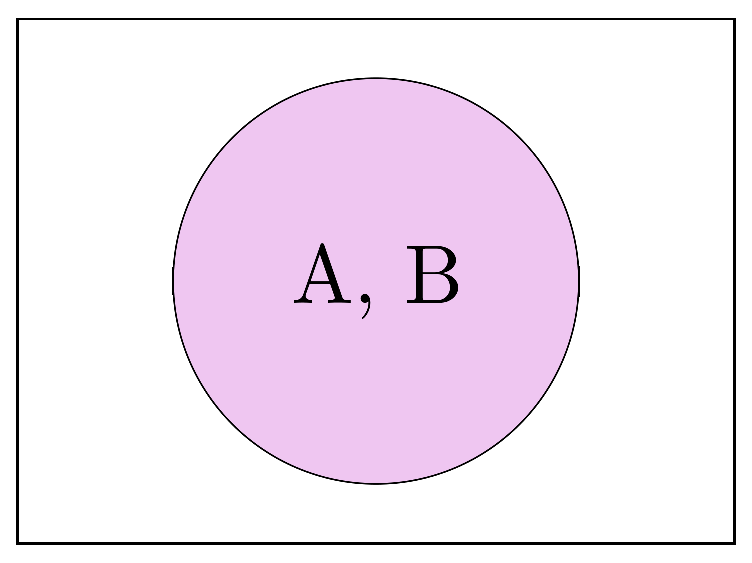
\includegraphics[width=0.2\textwidth]{discrete/sets/equal.eps}
  \end{center}
  \caption{$A=B$.}
\end{figure}
We have two ways to write an \textbf{empty set}.
We could write $\emptyset$ or $\{ \}$.

A set with only one element is called a \textbf{singleton set}.
\index{singleton set}

The set $A$ is a \textbf{subset}\index{subset} of set $B$ iff
\[ \forall x (x \in A \implies x \in B) \]
We then write $A \subseteq B$ to show that $A$ is a subset of $B$.
To demonstrate that $A$ is a subset of $B$, show that if $x$ belongs to $A$ then
it also belongs to $B$.
To show that $A$ is not a subset of $B$, that is, $A \not \subseteq B$, find a 
single element $x \in A$ such that $x \not \in B$.\footnote{\
    The symbol $\not \in$ means \emph{not in}.
}
\begin{figure}[H]
  \begin{center}
    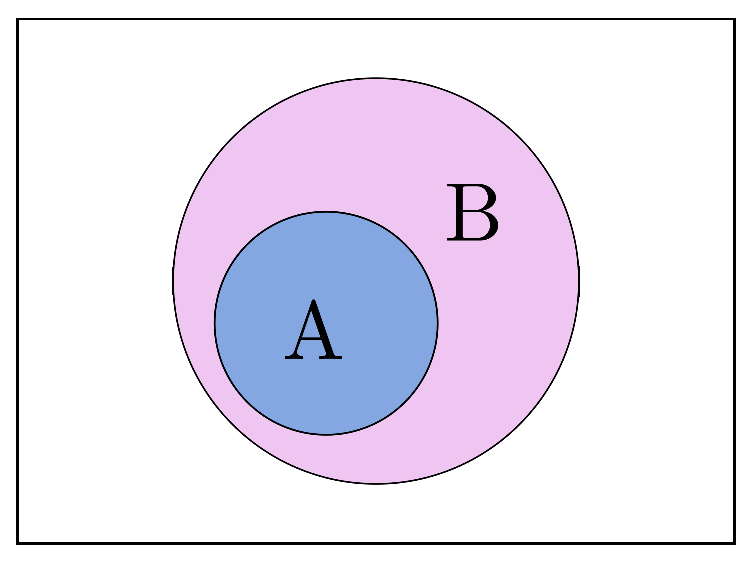
\includegraphics[width=0.2\textwidth]{discrete/sets/subset.eps}
  \end{center}
  \caption{$A\subseteq B$}
\end{figure}
If the set $A$ is a subset of the set $B$ but $A \neq B$, we write $A \subset B$ 
and say that $A$ is a \textbf{proper subset} of $B$.
That is, $A$ is a proper subset of $B$ iff
\[ \forall x (x \in A \implies x \in B) \land \exists x (x \in B \and x \not \in A). \]
This means, if the element $x$ exists in set $A$, then it also exists in set 
$B$, but there is at least one element $x$ in $B$ that is not in $A$.

\subsection{Set Operations}

For a set $A$ and a set $B$, the following operations apply:

The \textbf{cartesian product} of $A$ and $B$, denoted $A \times B$, is the set of
all ordered pairs $(a, b)$ where $a \in A$ and $b \in B$. Hence,
\[ A \times B = \big\{ (a,b) | a \in A \land b \in B \big\} \]

\begin{ex}
  Find $A \times B$ when $A = \{ 1,2 \} $ and $B = \{ a, b, c\} $.
  \begin{sol}
    \[A \times B = \big\{(1,a),(1,b),(1,c),
    (2,a),(2,b),(2,c)\big\}\]
  \end{sol}
\end{ex}

The \textbf{intersection}\index{intersection} of $A$ and $B$, denoted 
$A \cap B$,
is the set containing those elements in both $A$ and $B$, but not just one.
If the intersection of $A$ and $B$ is $\emptyset$, we say the two sets are 
\textbf{disjoint}.\index{disjoint}
\[ A \cap B = \big\{ x \in A | x \in B \big\}\]
\begin{figure}[H]
  \begin{center}
    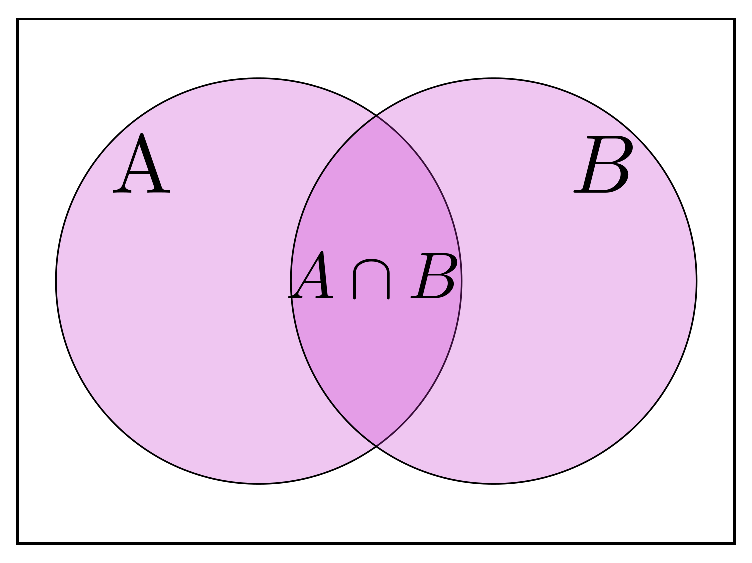
\includegraphics[width=0.2\textwidth]{discrete/sets/intersection.eps}
  \end{center}
  \caption{$A\cap B$}
\end{figure}The \textbf{union}\index{union} of $A$ and $B$, denoted $A \cup B$,
is the set containing all elements in either or both $A$ and $B$.
\[ A \cup B = \big\{ x | x \in A \lor x \in B \big\}\]
\begin{figure}[H]
  \begin{center}
    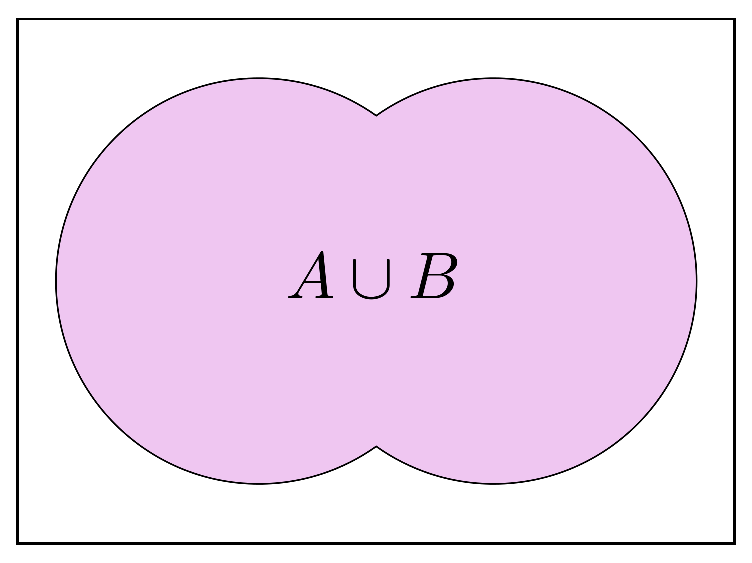
\includegraphics[width=0.2\textwidth]{discrete/sets/union.eps}
  \end{center}
  \caption{$A \cup B$}
\end{figure}
The \textbf{complement}\index{complement} of $A$ and $B$, denoted $A \setminus B$,
is the set containing those elements in $A$ but not in $B$.
It is sometimes called the \emph{component of $B$ with respect to $A$}.
This phrasing is used because the difference of $A$ and $B$ is different from the difference of $B$ and $A$.
\[ A \setminus B = \big\{ x \in A \big| x \not\in B \big\} \]

The \textbf{absolute complement}\index{absolute complement}
of $A$ is denoted $A^c$, and exists only if a universal set\footnote{A set containing all sets, including itself.}
$\mathbf{U}$ is defined, and is found by
\[ A^c = \mathbf{U} \setminus A.\]

\begin{table}
  \centering
    \begin{tabular}{>\(l<\) r}
      \textbf{Proposition} & \textbf{Name} \\ \hline\noalign{\smallskip}
      A \cap U = A & \multirow{2}{*}{identity laws} \\
      A \cup \emptyset = A \\\hline
      A \cup U = U & \multirow{2}{*}{domination laws} \\
      A \cap \emptyset = \emptyset \\\hline
      A \cup A = A & \multirow{2}{*}{idempotent laws} \\
      A \cap A = A \\\hline\noalign{\smallskip}
      \big(A^c\big)^c=A & involution law \\\noalign{\smallskip}\hline
      A \cup B = B \cup A & \multirow{2}{*}{commutative laws} \\
      A \cap B = B \cap A \\\hline
      A \cup (B \cup C) = (A \cup B) \cup C & \multirow{2}{*}{associative laws} \\
      A \cap (B \cap C) = (A \cap B) \cup C\\\hline
      A \cup (B \cap C) = (A \cup B) \cap (A \cup C) & \multirow{2}{*}{distributive laws} \\
      A \cap (B \cup C) = (A \cap B) \cup (A \cap C) \\\hline\noalign{\smallskip}
      \big(A \cup B\big)^c = A^c \cap B^c & \multirow{2}{*}{DeMorgan's laws} \\
      \big(A \cap B\big)^c = A^c \cup B^c \\\hline
      A \cup (A \cap B) = A & \multirow{2}{*}{absorbtion laws} \\
      A \cap (A \cup B) = A \\\hline
      A \cup A^c = U& \multirow{2}{*}{complement laws} \\
      A \cap A^c = \emptyset
    \end{tabular}
  \caption{Useful set identities.}
  \label{tab:setidentities}
\end{table}


\section{The Well-Ordering Principle}\index{well-ordering principle}
The \textbf{well-ordering principle} states that
\begin{theorem}
Every nonempty set of nonnegative integers has a smallest element.
\label{thm:wellordered}
\end{theorem}
We can use this to prove propositional statements associated with universal quantifiers.

To prove that
\[ \forall n \in \mathbb N \big( P(n)\big) \]
First, we define a set $C$ such that
\[ C : : = \big\{ n \in \mathbb N^+ \big| \neg P(n) \big\} \]
That is, we define the set $C$ to be the set of integers for which $P(n)$ is false.
We assume that this set is nonempty---that is, there is at least one nonnegative integer for which $P(n)$ is false.
By the well-ordering principle, there is a smallest element, $n$, in $C$.
From this, we reach a contradiction.
For example, we could show that $n$ can be used to find an element smaller than itself.
Now, we conclude that the set $C$ must be empty.

\begin{ex}
  Prove that the sum of all integers from $1$ to $n$ is \[\frac{n(n+1)}{2}.\]

  In basic algebraic notation, we could write this sum as
  \[1 + 2 + 3 + \cdots + n \]
  But we have a way of simplifying this using something called \textbf{sigma notation}\index{sigma notation}.
  We would write it as follows:
  \[1+2+3+\cdots+n  \sum_{1}^n \frac{n(n+1)}{2} \]
  \begin{proof}
    Now, we define a set $C$ such that
    \[ C : : = \bigg\{ n \in \mathbb N \big| \sum_{i=1}^n i \neq \frac{n(n+1)}{2}\bigg\}\]
    By the \emph{well-ordering principle}, $C$ has a smallest element, which we will call $c$.
    Since $c$ is the smallest counterexample,
    \[\sum_{i=1}^n = \frac{n(n+1)}{2}\]
    holds for all $n<c$ but not for $n=c$. So, that sum should hold for $c-1$:
    \begin{align*}
      1+2+3+\cdots+(c-1)&=\frac{(c-1)\big[(c-1)+1\big]}{2}\\
      1+2+3+\cdots+(c-1)&=\frac{(c-1)c}{2}\\
      1+2+3+\cdots+(c-1)&=\frac{c^2-c}{2}\\
      \intertext{Now, we add $c$ to both sides.}
      1+2+3+\cdots+(c-1)+c&=\frac{c^2-c}{2}+c\\
      \intertext{Simplify.}
      1+2+3+\cdots+(c-1)+c&=\frac{c^2-c}{2}+(c)\left(\frac{2}{2}\right)\\
      1+2+3+\cdots+(c-1)+c&=\frac{c^2-c+2c}{2} \\
      1+2+3+\cdots+(c-1)+c&=\frac{c^2+c}{2} \\
      \intertext{Factor out $c$ from the right-hand side.}
      1+2+3+\cdots+(c-1)+c&=\frac{c(c+1)}{2} \\
    \end{align*}
    Which means that
    \[\sum_{i=1}^n = \frac{n(n+1)}{2}\]
    holds for $c$, which contradicts our definition of $C$. Therefore $P(n)$ holds for all  $n \in \mathbb N$.
  \end{proof}
\cite{mcsfull}
\end{ex}

A few theorems come from the \emph{well-ordered principle}:\footnote{Proofs will come. From \cite[29]{mcsfull}.}
\begin{theorem}
  Any set of integers with a lower bound is well-ordered.
\end{theorem}
\begin{theorem}
  Any nonempty set of integers with an upper bound has a maximum integer.
\end{theorem}

\chapter{Recursion}\index{recursion}

\section{Recursive Definitions}

\begin{defn}\index{recursive form}
  \textbf{Recursive form} defines a set, an equation, or a process by defining a starting set or a value and giving a rule for continuing to build the set, equation, or process based on previously defined terms.
\end{defn}

The key for recursion is the \emph{rule for continuing to build} the set, equation, or process. This is what allows us to do the new element, new equation, or new process based on previously defined terms.

A recursive definition has two parts.

\begin{defn}
  In the \textbf{basis step}\index{basis step}, we must define values for some finite number of
  elements. For sets, we state the \emph{basic building blocks}\index{basic
  building blocks} of the set. for functions, state the values of the function
  on the basic building blocks.
\end{defn}
\begin{defn}
  The remaining elements in the recursive definition are defined by the
  \textbf{recurrence relation}\index{recurrence relation}. For sets, we show how
  to build new things from the old with some basic construction rules. For
  functions, we show how to compute the value of a function on the new elements
  of that set.
\end{defn}

\subsection{Recursively Defined Functions}\index{functions, recursively defined}

Let us create a recursive definition of the function $F$, defined on nonnegative integers. To give a recursive definition of $F$:
\begin{enumerate}\item \emph{Basis}. Specify F(0).
    \item \emph{Recursive step}. Give a rule for defining $F(n+1)$ from $F$ evaluated at smaller values.
\end{enumerate}
\begin{ex}
  \begin{align*}
    f(0) &= 1 \\
    f(n) &= f(n-1) +2
  \end{align*}
\end{ex}
\begin{ex}
  \begin{align*}
    g(0) &= 1 \\
    g(k+1) &= g(k)+2
  \end{align*}
\end{ex}
\begin{ex}
  \begin{align*}
    a_0 &= 1 \\
    a_n &= a_{n-1}
  \end{align*}
\end{ex}
\begin{ex}
  Find the recursive form of $n!$, the function given by
  \begin{equation}\label{eq:nfact}
   n!=\prod_{k=1}^n k \
  \end{equation}
  \begin{figure}[h]
    \begin{center}
      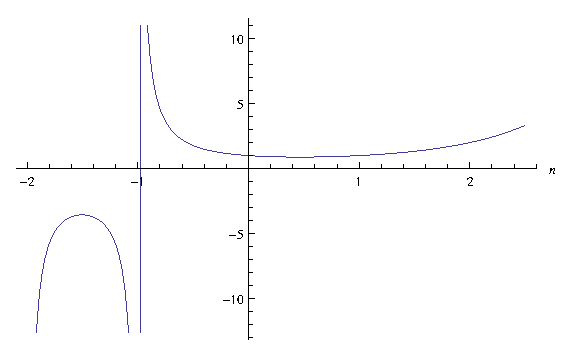
\includegraphics{discrete/recursion/nfact.eps}
    \end{center}
    \caption{A plot of $n!$. Its behavior is much harder to describe in the
    negatives, so we normally just treat it as having a domain of $n \geq 0$.}
    \label{fig:nfact}
  \end{figure}
  \begin{sol}
    The basis step in either the \emph{closed form} or \emph{recursive form}
    definition for $n!$ is that $0!=1$. In equation \eqref{eq:nfact}, it is implied
    under the convention that the product of no numbers at all is
    one\footnote{This is called the \textbf{empty product} or \textbf{nullary
    product}, and is responsible for providing the \emph{multiplicative
    identity} $1$.}

    So in order to define a recursive form for $n!$, we must start with the
    definition:
    \begin{equation}
      f(n) =
      \begin{cases}
        1 & \text{if }n=0
      \end{cases}
    \end{equation}

    Now that we have the basis step, to get the \emph{recursive step} we will
    look at a few instances of the factorial function:
    \begin{align*}
      f(0) &= 1 \\
      f(1) &= 1 \\
      f(2) &= 2 \\
      f(3) &= 6 \\
      f(4) &= 24 \\
      f(5) &= 120 \\
      & \vdots
    \end{align*}
    If we are careful, we'll notice that we can factor a $n$ from our result on
    each instance.
    \begin{align*}
      f(1) &= 1\cdot1 \\
      f(2) &= 2\cdot1 \\
      f(3) &= 3 \cdot 2 \\
      f(4) &= 4 \cdot 6 \\
      f(5) &= 5 \cdot 24 \\
      &\vdots
    \end{align*}
    We notice that $f(n)$, for any $n > 1$, is given by $n$ times the term
    before it. By writing this out, we get our \emph{recursive definition for
    factorials}.
    \begin{equation}
      f(n) =
      \begin{cases}
        1 & \text{if }n=0 \\
        n \times f(n-1) & \text{if }n > 0
      \end{cases}
    \end{equation}
    As is the case with factorials, \emph{recursive form} often offers the
    advantage that it is very intuitive for humans to understand. Its downside is
    that it is very seldom computationally faster than its \emph{closed-form}
    alternative. For this reason, we should attempt to find closed-form
    solutions to recursive definitions where possible or necessary.

    Generally speaking, given a recursive function on a test, we should be able to find a
    closed-form representation and vice-versa.
  \end{sol}
\end{ex}
\begin{ex}
  Find a recursive definition of the \textbf{Fibonacci sequence}\index{Fibonacci
  sequence}:
  \[ 1, 1, 2, 3, 5, 8 13, 21, 34, \ldots \]
  \begin{figure}[h]
    \begin{center}
      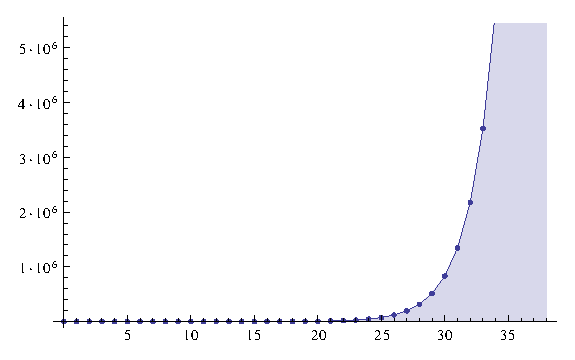
\includegraphics{discrete/recursion/fibonacci.eps}
    \end{center}
    \caption{A plot of the Fibonacci sequence.}
    \label{fig:fibonacci}
  \end{figure}

  The Fibonacci sequence is often explained using the analogy of rabbits on an
  island.
  \begin{quote}
    ``A young pair of rabbits (one for each sex) is placed on an island. After
    they are 2 months old, each pair of rabbits produces another pair each month.
    The number of pairs of rabbits after $n$ months is $f(n)$.''
  \end{quote}
  \begin{sol}
    Notice that we need \textbf{two} initial conditions to define this
    recurrence relation.
    \begin{equation}
      f(x) =
      \begin{cases}
        1 & \text{for }0 \leq x \leq 1 \\
        f(n) + f(n-1) &\text{for } x > 1
      \end{cases}
    \end{equation}
  \end{sol}
  \begin{note}
    This definition requires two initial conditions. It is very important in recursive definitions to have the right number of initial conditions.
  \end{note}
\end{ex}
%\begin{ex}
%  Give a recursive definition of
%  \[ F(n) = a^n \]
%
%  \begin{tabular}{ll}
%    $f(0)=a^0=1$ & basis \\
%    $f(n)=a\cdot f(n-1)$& recursion \\
%  \end{tabular}
%  \begin{note}
%    \[f(n)=a^n=\underbrace{a \cdot a \cdot a \cdot \dots a}_{n}\]
%
%    \[f(n-1)=a^{n-1}=\underbrace{a \cdot a \cdot a \cdot \dots a}_{n-1}\]
%  \end{note}
%\end{ex}
%\begin{ex}
%  Give a recursive definition of
%  \[ F(n) = \sum^{n}_{k=0} a_k \]
%
%  \begin{tabular}{ll}
%    $f(c)=a_0$ & basis \\
%    $f(n)=f(n-1)+a_n$ & recursion \\
%  \end{tabular}
%  \begin{note}
%    \[ F(n) = \sum^{n}_{k=0} a_k=a_0+a_1+\dots+a_{n-1}+a_n \]
%  \end{note}
%\end{ex}
%
%\begin{comment}
%\begin{ex}
%  \begin{tabular}{ll}
%    Basis. & $f(0)=100,000=A$ \\
%    Recursion. & $f(k)=f(k-1)+f(k-1)*4\%$ \\
%    & $f(k) = (1+\alpha)(f(k-1))$ \\
%  \end{tabular}
%  \begin{tabular}{ll}
%
%  \end{tabular}d
%  \end{ex}
%\end{comment}
%
%  Mathematical induction is a way to varify the correctness of a recursive definition.
%
%  \begin{ex}
%    \begin{align*}
%      a_1&=1 \\
%      a_n&=2a_{n-1}+1 \text{ for all integers n $\geq 2$}
%      \intertext{Then prove by induction:}
%      a_n&=2^n-1 \text{ for all } n \geq 1
%    \end{align*}
%    \begin{tabular}{ll}
%      & $a_1=2^1-1=1=a_1 \text{ by recursion}$\\
%      & If $a_n=2n-1$, then $a_{n+1}=2^{n+1}-1$. \\
%      & assume $a_n=2^n-1$ \\
%      & $a_{n+1}=2a_n+1=2(2^n-1)+1$ \\
%      & $= 2 \cdot 2^n -2 +1 = 2^{n+1}-1$
%    \end{tabular}
%  \end{ex}
%
%\section{Recursive Algorithms}
%
%Recursive algorithms are only used because certain algorithms are recursive in nature. Recursion does not save any computational power. For most algorithms, we can define a non-recursive version. However, sometimes it is inconvenient to find a non-recursive equivalent to a recursive algorithm.
%
%A recursive algorithm is one which calls itself to sove ``smaller'' versions of an input problem. Some algorithms are recursive in nature, like the binary search or Fibonacci sequence.
%
%The current status of the algorithm is placed on the \emph{stack}. A stack is a data structure from which entries can be added and deleted only from one end.
%
%\begin{verbatim}
%  procedure factorial(n)
%    if n < 0 return 'error'
%    if n = 0 the nreturn 1
%    else
%      return (n*factorial(n-1))
%\end{verbatim}
%
%Say we want to calculate $f(3)$.
%
%\begin{align*}
%  f(3)=3 \cdot &f(2)&&\\
%  &\to f(2) = 2 \cdot f(1)&\\
%  &&\to f(1)=1\cdot &f(0)\\
%  &&&\to f(0)=1
%\end{align*}
%
%
%

\chapter{Counting}

We can use counting techniques to determine the complexity of an algorithm.
Counting is very important not only for computer science but also for any job.
For example, counting problems are common in job interviews to see how a potential employee reacts.

Counting, ultimately, is a very simple theoretical process governed by some basic rules.

\section{Rules of Counting}

\subsection{The Sum Rule}\index{sum rule for counting}
  If a first task can be done in \(n_1\) ways and a second task can be done in \(n_2\) ways,
  and if these tasks cannot be done at the same time, then there are \(n_1+n_2\) ways to do either task.

  In set notation: if \(A\) and \(B\) are \emph{disjoint}, then \(|A \cup B|=|A|+|B|\).

\subsection{The Product Rule}\index{product rule for counting}

Suppose that a procedure can be broken down into two tasks.
If there are \(n_1\) ways to do the first task and 
\(n_2\) ways to do the second task
\emph{after} the first task has been done,
n there are \(n_1n_2\) ways to do the procedure.

In set notation:
\[|A \times B| = |A||B| \]

\subsection{Examples}

\begin{ex}
  Let \(D = \{x, y, z\}\). Let \(R=\{1,2,3,4,5\}\).
  \begin{itemize}
    \item[a) ] How many functions are there from \(D\to R\)?
    \item[b) ] How many \emph{one-to-one} functions are there?
    \item[c) ] How many onto functions are there?
  \end{itemize}
  \begin{sol}
    We only have two rules for counting right now.
    For the product rule, we must assume we are going to define mapping for \(x\), then for \(y\), then for \(z\).
    With the sum rule, then we can define mapping for \(x\), or \(y\), or \(z\).

    Then we go back to ``how do we define the function?'' Do we have to find a mapping for every element in the domain?

    Yes. By definition of functions, we must.


    \begin{itemize}
      \item[a) ] There are \(5 \times 5 \times 5\) possible mappings from \(D \to R\).
      \item[b) ] \(5\times4\times3\).
      \item[c) ] It is impossible for the function to be onto. There are not enough elements in the domain to have values in the range to map to them.:w
    \end{itemize}
  \end{sol}
\end{ex}
\begin{ex}
  A typical PIN is a sequence of any four numbers chosen form the 26 letters and the ten digits.
  \begin{itemize}
  \item[a) ] How many different PINs are possible if repetition is allowed?
    \item[b) ] What if repetition is not allowed?
  \end{itemize}
  \end{ex}
\begin{ex}
  The ASCII character set is represented by 7 binary bits. How many characters are there in the set?
  % \begin{sol}
  %  We have to make seven choices in sequence to come up with an ASCII character.
  %  For each choice, we have two choices.
  % \end{sol}
\end{ex}
\begin{ex}
  Count the number of binary bit strings of length 4 or less.
\end{ex}
\begin{ex}
  A student can choose a computer project from one of three lists. The three lists contain 10, 20, or 30 possible projects. There is no overlap among that list. How many projects are there to choose from?
  \begin{sol}
    \[10+20+30 \text{ projects}\]
  \end{sol}
\end{ex}

\section{The Pidgeonhole Problem}\index{pidgeonhole problem}
\begin{quote}
  A flock of 13 pideons roosts in a set of 12 pidgeonholes. One of the
  pidgeonholes must have more than one pidgeon.
\end{quote}
If $k$ is a positive integer and $k+1$ objects are placed into $k$ boxex, then
at least one box must have more than one object.
\begin{proof}
  We can prove this by contradiction. Suppose all of the pidgeons fit in to $k$
  boxes exclusively. Therefore, there must be $k$ pidgeons, which is not equal
  to $k+1$.
\end{proof}
\begin{corollary}
  A function $f$ from a set with $k+1$ elements to a set with $k$ elements is
  not \emph{one-to-one}.
  \begin{proof}
    Say we have eight boxes. We want to divide the objects evenly among the
    boxes, so we place $2$ in each box. The number of boxes over the number of
    elements is equal to $2$ objects per box.

    For nine boxes, we must take the ceiling function of $9/4$ and find 3.
  \end{proof}
\end{corollary}
\begin{theorem}
  \label{th:pidgeonhole}
  If $N$ objects are placed into $k$ boxes, then there is at least one box
  containing at least $N/K$ objects.
\end{theorem}
\begin{ex}
  Among 100 people there are at least [100/12]=9 who were born in the same
  month.
\end{ex}
\begin{ex}
  How many cards must be selected from a standard deck of 52 cards to guarantee
  that at least three cards of the same suit are selected. After generalizing
  the pidgeonhole problem, we find that at least one box contains at least
  $[N/4]$ cards. At least three cards of one suit are selected 
\end{ex}
\section{Combination Rule}

For the addition rule, we know the values and don't know the positions.
Where we know the position and don't know the values, we use the combination
rule to solve the problems.

For the rule of products, things are more general. We can select the same
elements, and we are determining value rather than location.

\begin{ex}
  How many bit strings of length $100$ have at least $2$ ones?
  \begin{sol}
    The solution is given by the combination rule:
    \[ C(100 2) \]
    For exactly 3 ones, we do
    \[ C(100, 3) \]
    One hundred $1$s:
    \[ C(100,100) \]
    Or
    \[ C(100, 2) + C(100, 3),+ \cdots + C(100,100) \]
    We can do this using the combination rule as follows:
    \[ 2^{100} - C(100,0) - C(100,1) \]
    which is the total number of bit strings with at least 2 ones.
  \end{sol}
\end{ex}

\section{Counting the Complement}

This is an applicaiton of the set decomposition principle, which states that the
total number of objects is equal to the number of objects that have a certain
property plus the number of objects that do not have the property.
\begin{ex}
  Passwords of lenght 8 are made of lowercase letters and decimal digits. How
  many of such passwords contain at least one decimal digit?
  
  In the past, we solved this as follows:
  \[ (26+10)^8 = \text{ number of passwords with more than one digit} + 26^8 \]

  The combination rule will tell us:location of digit -> value of digit ->
  value of letters


  Number of passwords with one digit:
  \[ C(8,1) \times 10 \times 26^7 \]
  The number of passwords with two digits:
  \[ C(8,2)\times10^2\times26^6 \]
  And so on. The sum of these numbers provides our answer.
\end{ex}

\section{The Binomial Theorem}
\begin{ex}
  Find the expansion of
  \[(x+y)^2,\, (x+y)^3\]
  \begin{sol}
    \[(x+y)^2 = x^2 + 2\times y+ y^2\]
    That is to say,
    \[ C(2, 0)+ C(2, 1)+ C(2,2) \]
    For
    \[(x+y)^3\]
    we get
    \begin{align*}
      (x+y)^3&=C(3,0)+C(3,1)+C(3,2)+C(3,3) \\
      &= x^3 + 3x^2 y + 3 x y^2 + y^3
       &= (x+y)(x+y)(x+y)
    \end{align*}
  \end{sol}
\end{ex}
This gives us the \textbf{binomial theorem}.
\[ (x+y)^n = \sum^n_{j=0} C(n, j)x^{n-j}y^j \]
\begin{ex}
  What is the coefficient of $x^{25}y^{75}$ in the expansion of $(2x-5y)^{100}$?
  \begin{sol}
    Let $2x=a$ and $5y =b$.
    \[ (a+b)^n= \sum^n_{j=0} C(n,j) a^{n-j} b^j \]
    Now we solve for the variables. We know $a$, $b$, and $n$, so we must solve for
    $j=75$.
    Now, we put together our sum.
    \[ C(100,75)(2x)^{100-75}(-5y)^{75} \]
    \[ = C(100,75) 2^{25} \cdot x^{25} \cdot (-5)^{75} \cdot y^{75} \]
    Which makes our answer
    \[ C(100, 75) \cdot 2^{25}\cdot(-5)^{25}\]
  \end{sol}
\end{ex}
\begin{homework}
  Section $6.3$ (p.413): $17,20,33,34,37$.
  Section $6.4$ (p.421): $3, 5, 9$.

  On Monday, we will get the even numbered answers for sections $6.1-6.4$,
  around six or seven questions. We will also receive the review question
  answers. This homework will be due on Tuesday, along with a quiz on counting.
  Review the self-assessment on the counting sction.
\end{homework}

\input{discrete/numbers}

\part{Mathematical Analysis}
\setcounter{section}{0}
\chapter{Basics of Functions}
\section{Definition of a Function}
\begin{defn}
    A \textbf{function} $f$ from a set $D$ to a set $R$ is an assignment of exactly one element $f(x) \in R$ to each element $x \in D$.
    if $f$ is a function from $D$ to $R$, we write
    \begin{equation}
        f:D \to R,
        \label{eq:function_definition}
    \end{equation}
    and say that $f$ \emph{maps} $D$ to $R$.\footnote{Sets and set builder notation are explained in more detail in \chref{ch:sets}.}
    \index{function}
\end{defn}
\begin{figure}[h]
    \centering
    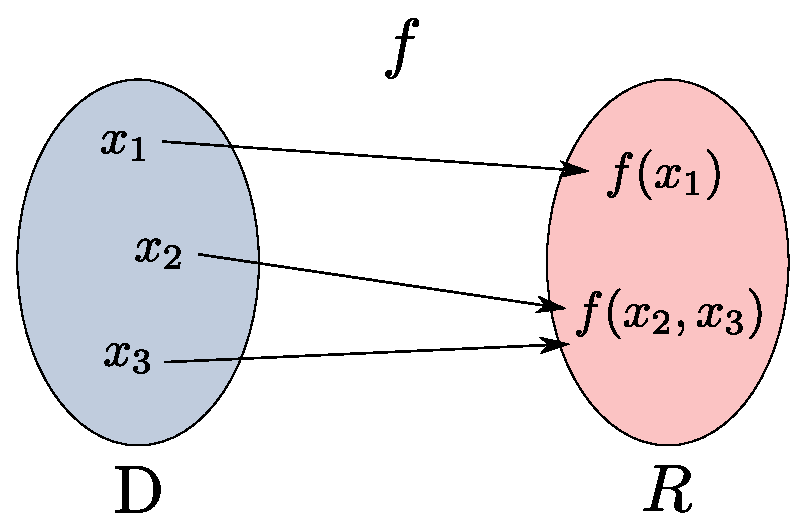
\includegraphics[width=0.4\textwidth]{continuous/functions/function.eps}
    \caption{A function $f$ mapping from $D$ to $R$. Note how multiple $x$ 
        values share the same $f(x)$ value.}
    \label{fig:function}
\end{figure}

One technique that can help us understand functions is by describing them with words,
including mathematical language.
We can discuss the behavior of a function in general,
describing its properties, or we can discuss its behavior in more specific terms,
like when we evaluate a function at a certain value.

We can also talk about functions using visual language, as in graphs, arrow 
diagrams, and tables.
% There are, of course, many ways to visually represent a function, but for our purposes these will prove the most useful.
% This includes some numerical displays of functions, like with a table of values.
% We can consider tables to be a visual description of a function because they combines visual formatting with descriptive data to produce a figural representation of a function's properties.

We will find graphs, in conjunction with the respective mathematical language, 
to be the most cohesive way to represent functions.
We should therefore attempt to be able to graph our functions whenever we wish to achieve the best possible understanding of them.

We will combine these techniques in an effort to paint a complete picture of its 
behavior.

\section{Properties of Functions}

Here, we will discuss a number of the properties that will be of interest when we
are describing functions.
Not all of these properties will exist for every type of function.
For example, not all functions will have an inverse 
(described in \secref{sec:inverse}), 
but the nonexistence of an inverse then becomes an important property of the 
function. % WHEN????? Tell the reader where this is useful.

\subsection{Domain and Range}

\begin{defn}
    The set $D$ of all possible input values is called the \textbf{domain} of 
    the function.
    \index{domain}
\end{defn}

\begin{defn}
    The set of all values $f(x)$ as $x$ varies throughout $D$ is called 
    the \textbf{range} of the function,
    representing the output value of $f$ at $x$.
    \index{range}
\end{defn}

\begin{defn}
    The \textbf{natural domain} of a function is the largest set of real 
    $x$-values for which a function returns real $y$-values.
    A function is said to be \textbf{real-valued} when $D = \mathbb{R}$.
\end{defn}
That is, the domain is equal to to the set of real numbers.
This means that we can put an arbitrary real number into the function and it 
will return a real $y$-value.

 \begin{remark}
     When we define a funciton $y=f(x)$ with a formula and the domain is not 
     stated explicitly or restricted by context, the domain is assumed to be the 
     \emph{natural domain}.
   \end{remark}
   \index{natural domain}

  The \textbf{vertical line test} for a function is based on the idea that if 
  $a$ is in the domain of the function $f$ then the vertical line $x=a$ will 
  intersect the graph of $f$ at a single point $ \big(a,f(a)\big)$.
  \index{vertical line test}

\begin{figure}[H]
  \begin{center}
    \subfigure[This passes the vertical line test]{\
      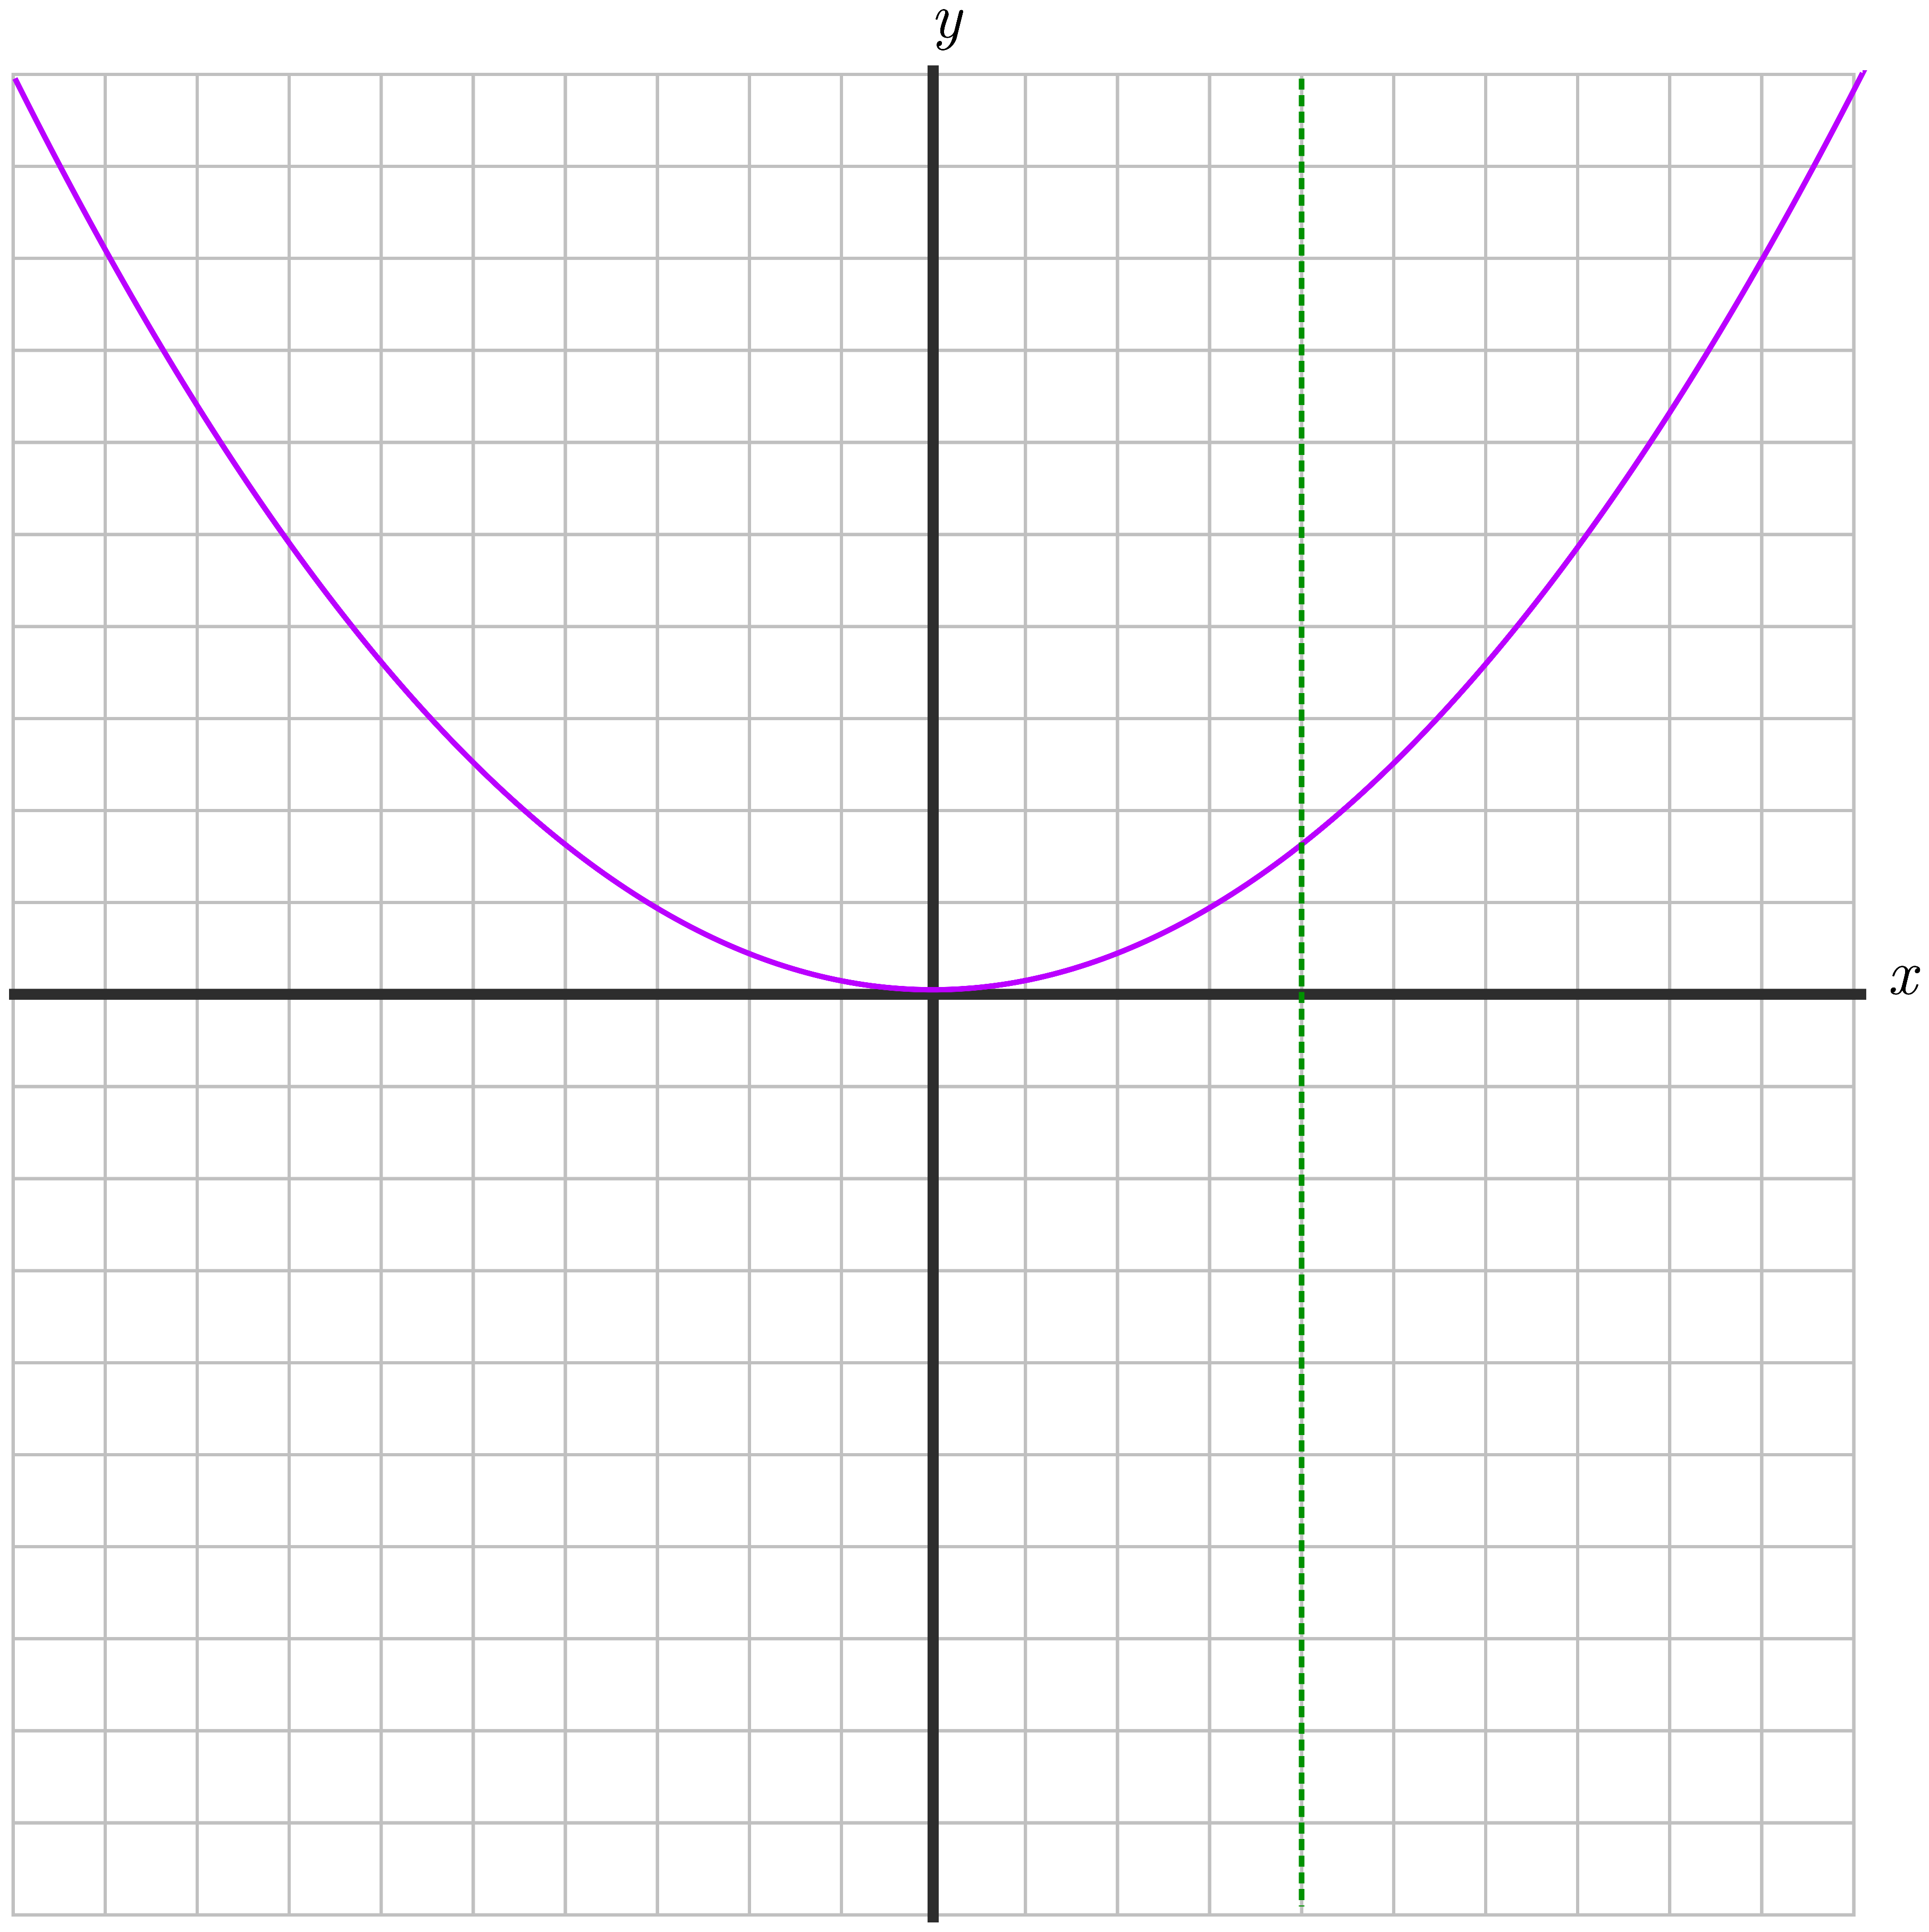
\includegraphics[width=0.4\textwidth]{continuous/functions/vlt1}
    }
    \subfigure[This fails the vertical line test]{\
      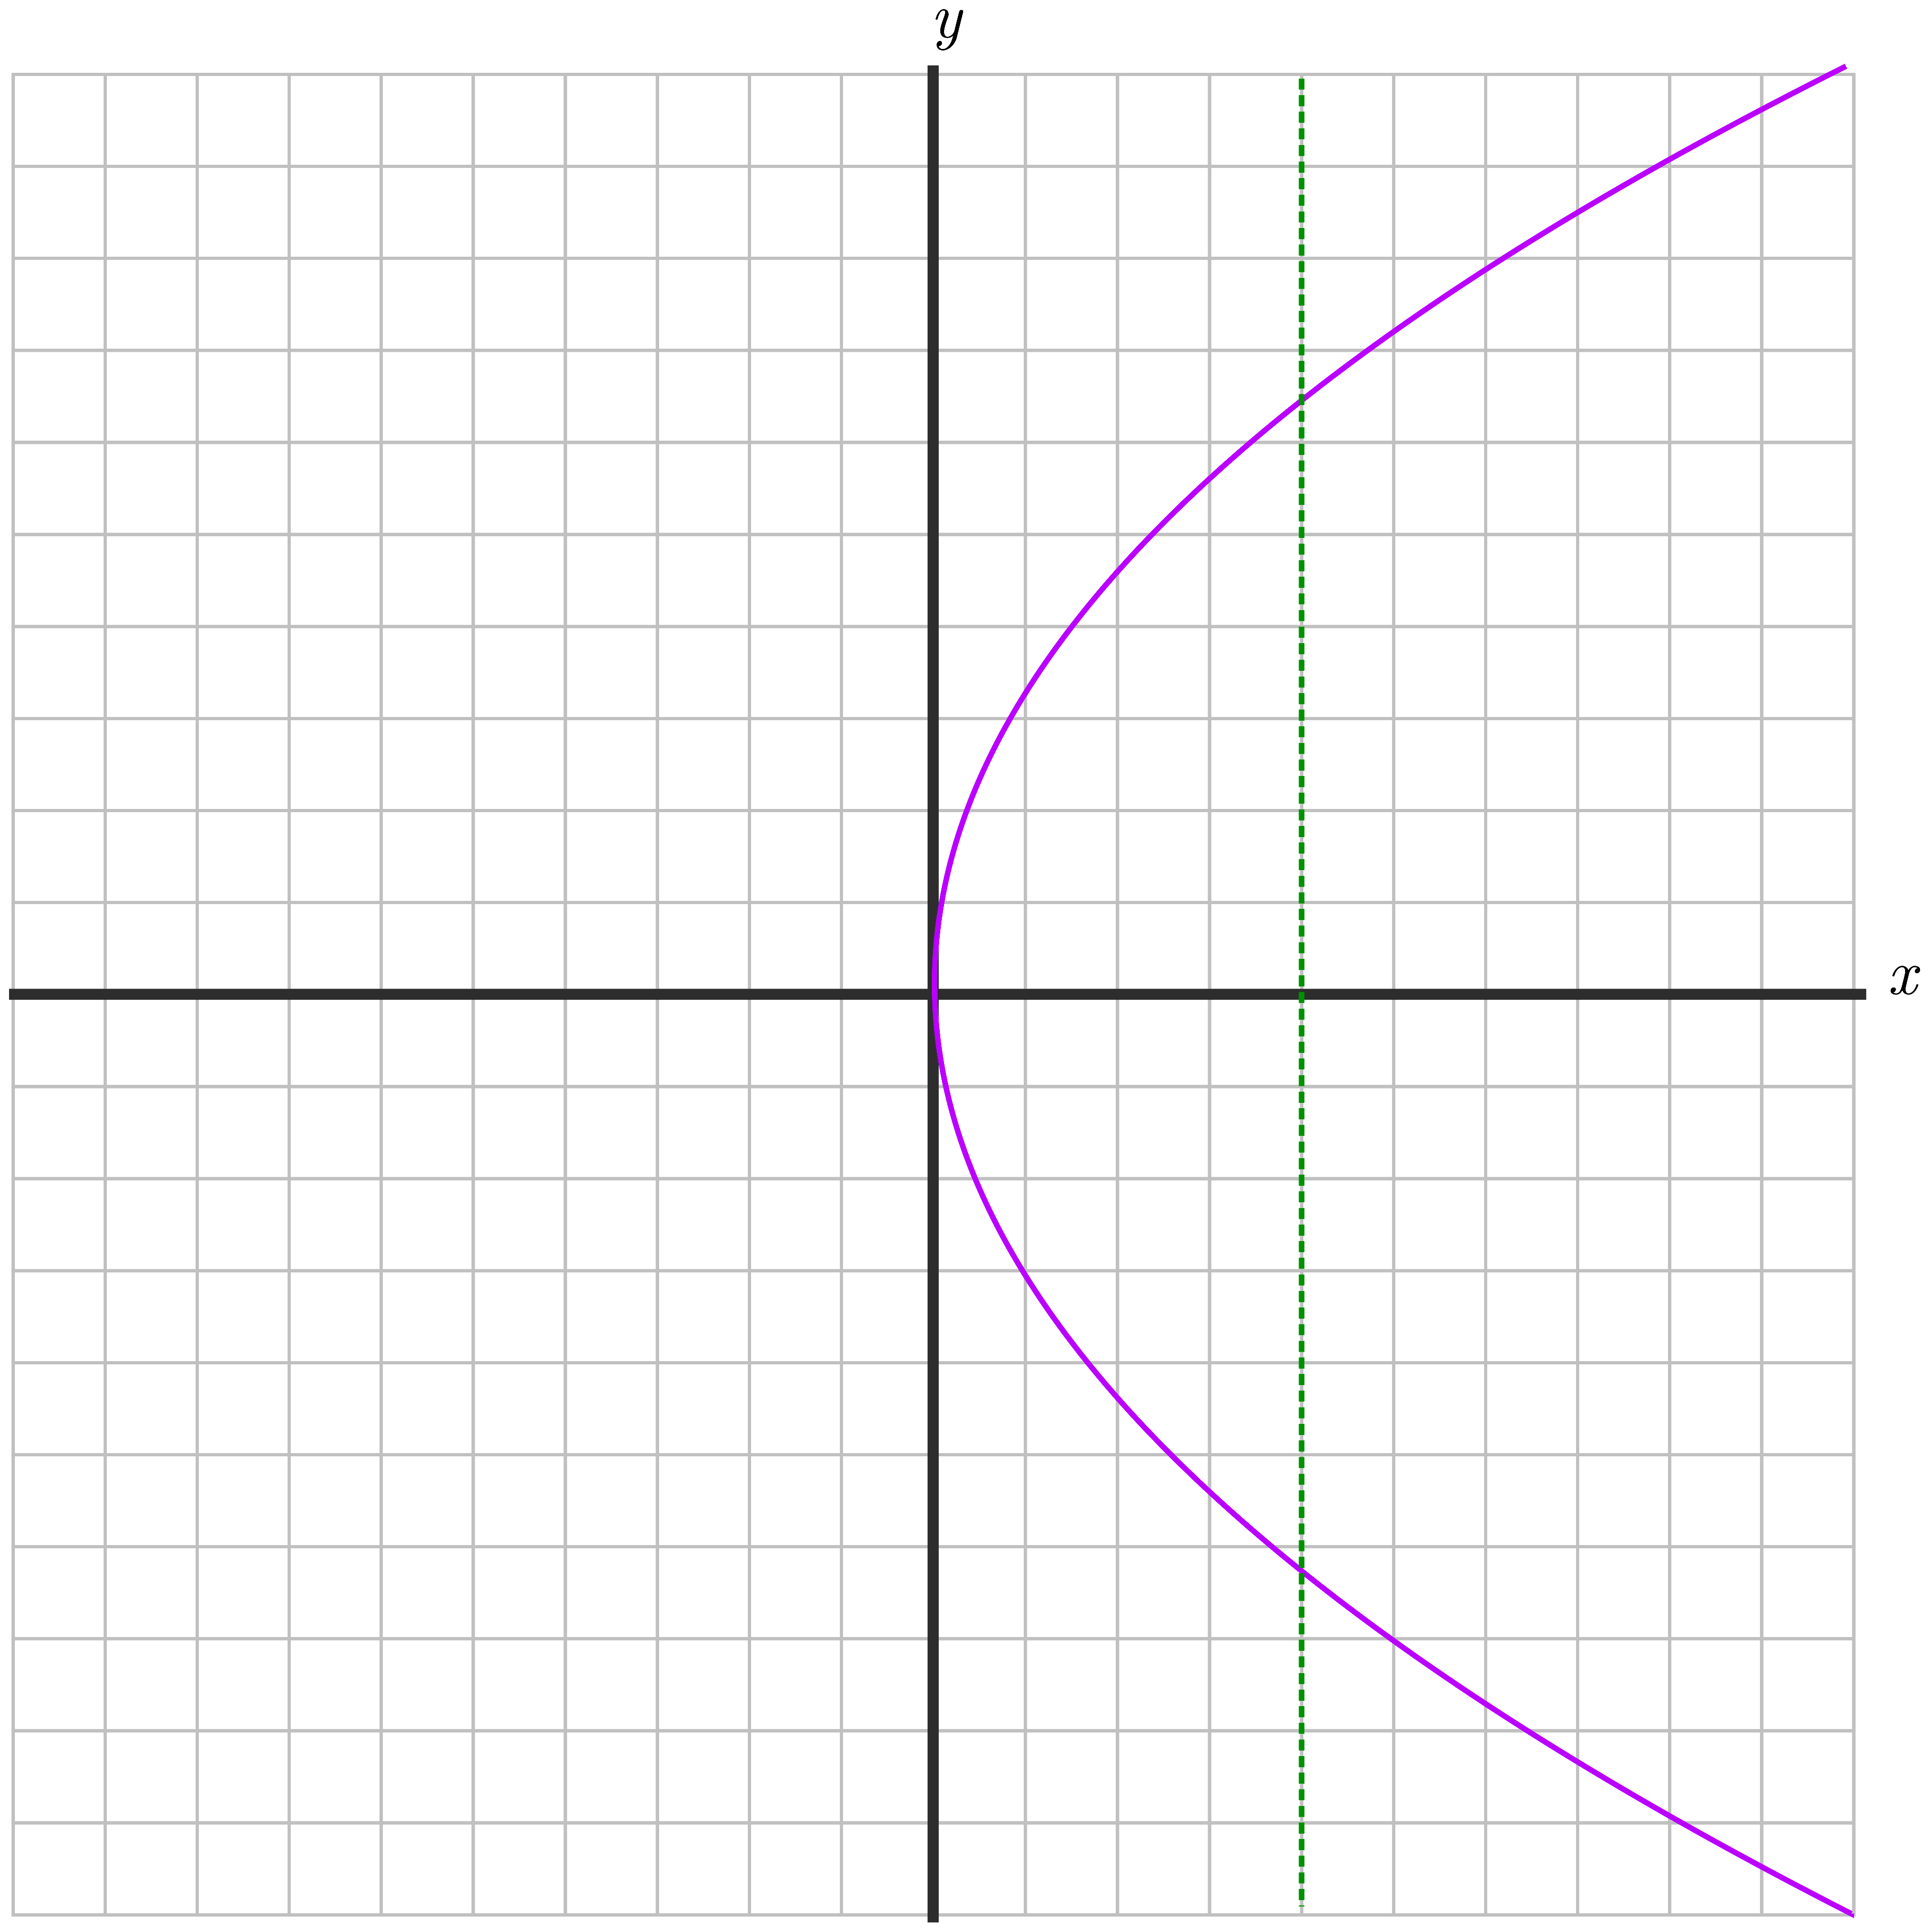
\includegraphics[width=0.4\textwidth]{continuous/functions/vlt2}
    }
  \end{center}
  \caption{Examples of the vertical line test.}
\end{figure}


\subsection{Dependent and Independent Variables}
  The letter $x$ in the notation $y=f(x)$ is called the 
  \textbf{independent variable} of the function, representing the input value 
  of $f$.
  \index{independent variable}

  The letter $y$ in the notation $y=f(x)$ is called the 
  \textbf{dependent variable}.
  It varies with respect to change in the dependent variable of the function.
  \index{dependent variable}

\subsection{Even and Odd Functions}

For a function $f$ in the form $y=f(x)$, we describe its type of symmetry by 
calling the function \textbf{even}\index{even functions} or 
\textbf{odd}\index{odd functions}.

An \textbf{even function} means $f(-x)=f(x)$.
An example of an even function is the function $f(x)=x^2$.
  \begin{figure}[H]
    \begin{center}
      \begin{tikzpicture}
        \begin{axis}[
            ylabel={$f(x)=x^2$},
            axis x line=bottom,
            axis y line=center,
            tick align=outside,
            yticklabels={,,}
            xticklabels={,,}
            xtickmax=10,
          ]
          \addplot[smooth,red]{x^2};
        \end{axis}
      \end{tikzpicture}
    \end{center}
    \caption{$f(x)=x^2$ is an \emph{even function}.}
  \end{figure}
  An \textbf{odd function} means $f(-x)=-f(x)$. An example of this is the 
  function $f(x)=x^3$.
  \begin{figure}[H]
    \begin{center}
      \begin{tikzpicture}
        \begin{axis}[
            ylabel={$f(x)=x^3$},
            axis x line=bottom,
            axis y line=center,
            tick align=outside,
            yticklabels={,,}
            xticklabels={,,}
            xtickmax=10,
          ]
          \addplot[smooth,red]{x^3};
        \end{axis}
      \end{tikzpicture}
    \end{center}
    \caption{$f(x)=x^3$ is an \emph{odd function}.}
  \end{figure}
\subsection{Surjective, Injective, and Bijective Functions}

\begin{defn}
  \index{one-to-one}
  \index{injective}
  If each $f(x)$ value produced by a function $f$ can only be obtained by one 
  unique $x$ value, then we say $f$ is \textbf{injective}, or 
  \textbf{one-to-one}.

  $ f: D \to R $ is injective or one-to-one iff
  \[
    \forall{(x_1 \wedge x_2 \in D)}
    \big[f(x_1)=f(x_2)
    \to x_1=x_2\big].
  \]
  \begin{remark}
    This also means that for injective functions,
    $ x_1 \neq x_2 \to f(x_1) \neq f(x_2)$.
  \end{remark}
\end{defn}
\begin{figure}[H]
    \begin{center}
        \subfigure[The function $f(x)=x^2$ is not \emph{one-to-one} because 
        there are two possible $x$-values that can produce each given 
        $y$-value.]
        {\
          \begin{tikzpicture}
            \begin{axis}[
                ylabel={$f(x)=x^2$},
                axis x line=bottom,
                axis y line=center,
                tick align=outside,
                yticklabels={,,}
                xticklabels={,,}
                xtickmax=10,
              ]
              \addplot[smooth,red]{x^2};
            \end{axis}
          \end{tikzpicture}
        }
        \hspace{0.2in}%
        \subfigure[The function $f(x)=x^3$ is \emph{one-to-one} because every 
        given $y$-value is mapped from a unique $x$-value.]
        {\
          \begin{tikzpicture}
            \begin{axis}[
                ylabel={$f(x)=x^3$},
                axis x line=bottom,
                axis y line=center,
                tick align=outside,
                yticklabels={,,}
                xticklabels={,,}
                xtickmax=10,
              ]
              \addplot[smooth,blue]{x^3};
            \end{axis}
          \end{tikzpicture}
        }
    \end{center}
  \end{figure}
  A function $y=f(x)$ is one-to-one iff its graph intersects each horizontal 
  line at most once.\index{horizontal line test}
\begin{defn}
  \index{onto}
  \index{surjective}
  $f: D \to R $ is \textbf{surjective} or \textbf{onto} iff
    \[\forall (y \in R) \exists  (x \in D) \big[f(x)=y\big]. \]
\end{defn}
\begin{figure}[H]
    \begin{center}
        \subfigure[The function $f(x)=x^2$ is not \emph{surjective} because 
        the values $(-\infty, 0)$ are never reached in its range.]
        {\
          \begin{tikzpicture}
            \begin{axis}[
                ylabel={$f(x)=x^2$},
                axis x line=bottom,
                axis y line=center,
                tick align=outside,
                yticklabels={,,}
                xticklabels={,,}
                xtickmax=10,
              ]
              \addplot[smooth,red]{x^2};
            \end{axis}
          \end{tikzpicture}
        }
        \hspace{0.2in}%
        \subfigure[The function $f(x)=x^3$ is \emph{one-to-one} because all $y$ values from $-\infty, \infty)$ have corresponding $x$-values.]
        {\
          \begin{tikzpicture}
            \begin{axis}[
                ylabel={$f(x)=x^3$},
                axis x line=bottom,
                axis y line=center,
                tick align=outside,
                yticklabels={,,}
                xticklabels={,,}
                xtickmax=10,
              ]
              \addplot[smooth,blue]{x^3};
            \end{axis}
          \end{tikzpicture}
        }
    \end{center}
  \end{figure}

  \begin{defn}
    \index{bijective}
    A function $f:A \to B$ is \textbf{bijective} iff it is \emph{both injective and surjective}.
  \end{defn}
\begin{figure}[H]
    \begin{center}
        \subfigure[The function $f(x)=x^2$ is not bijective.]
        {\
          \begin{tikzpicture}
            \begin{axis}[
                ylabel={$f(x)=x^2$},
                xlabel={$x$},
                axis x line=bottom,
                axis y line=center,
                tick align=outside,
                yticklabels={,,}
                xticklabels={,,}
                xtickmax=10,
              ]
              \addplot[smooth,red]{x^2};
            \end{axis}
          \end{tikzpicture}
        }
        \hspace{0.2in}%
        \subfigure[The function $f(x)=x^3$ is bijective.]
        {\
          \begin{tikzpicture}
            \begin{axis}[
                ylabel={$f(x)=x^3$},
                xlabel={$x$},
                axis x line=bottom,
                axis y line=center,
                tick align=outside,
                yticklabels={,,}
                xticklabels={,,}
                xtickmax=10,
              ]
              \addplot[smooth,blue]{x^3};
            \end{axis}
          \end{tikzpicture}
        }
    \end{center}
  \end{figure}


\subsection{Graphs} \index{graphs}

\begin{defn}
  \index{graph}
    If $f$ is a function with a domain $D$, then its \textbf{graph} is the set
    \[ \Big\{ \big( x,f(x) \big) \Big | x \in D \Big\},\]
    that is, it is the set of all points $(x, f(x))$ where $x$ is in the domain of the function.%
\footnote{Here, the difference between the words \emph{graph} and \emph{plot} is sometimes confusing. Technically speaking, a \emph{graph} is the set defined explicitly here, while a function's \emph{plot} refers to any pictorial representation of a data set. However, since the usage is inconsistent in this text, these formal definitions will usually not apply. It can be safely assumed that as long as we are within the realm of real numbers, all uses of either \emph{graph} or \emph{plot} hereafter simply refer to the pictorial representation of a function's graph in the form of a curve on the cartesian plane.}
\end{defn}

If $ (x,y) $ is a point on $f$, then $y=f(x)$ is the height of the graph above point $x$.
This height might be positive or negative, depending on the sign of $f(x)$.
We use this height relationship to plot functions.
\begin{figure}[H]
    \begin{center}
        \begin{tikzpicture}
          \begin{axis}[
              ylabel={$f(x)$},
              xlabel={$x$},
              axis x line=bottom,
              axis y line=center,
              tick align=outside,
              yticklabels={,,}
              xticklabels={,,}
              xtickmax=10,
            ]
            \addplot[smooth,red]{x+2};
          \end{axis}
        \end{tikzpicture}
      \caption{A plot of the function $f(x)=x+2$}
    \end{center}
  \end{figure}

\section{Composition of Functions}
\label{sec:compositefunctions}
\begin{defn}
  If $f$ and $g$ are functions, then the \textbf{composite} function 
  $f \circ g$, ``$f$ composed with $g$'', is defined by
  \[ (f \circ g)(x)=f\bigl(g(x)\bigr) \text{.} \]
  \begin{remark}
    The domain of $ f \circ g $ consists of the numbers $x$ in the domain of 
    $g$ for which $g(x)$ lies in the domain of $f$.
    See figure~\ref{fig:p1sin1x} for an example of a function which produces 
    indefinite $y$-values for real $x$-values around $x=0$.
  \end{remark}
  \index{composition}
\end{defn}
\begin{ex}
  If
  $f(x)=x^2$
  and
  $g(x)=1-\sqrt{x}$,
  find $ (f \circ g)(x) $ and $ (g \circ f)(x)$.
  \begin{sol}
      We know that $(f \circ g)(x)$ is just $f(g(x))$ so
      \[ f(g(x)) = (1 - \sqrt x )^2. \] For $(g \circ f)(x)$ it is the opposite
      and \[ g(f(x)) = 1 - \sqrt{x^2} ,\]
      which is equivalent to saying \[ g(f(x)) = 1 - \abs{x}. \]
  \end{sol}
\end{ex}

\section{Inverse Functions}\index{inverse functions}\label{sec:inverse}
An inverse function undoes, or inverts, the effects of an original function.
% Old gibberish from when this was in the transcendental section.
%While inverse functions are not, by definition, transcendental, we will look 
%at them in this chapter because they are useful for producing inverse 
%trigonometric functions--functions that are transcendental.
They are useful for producing inverse trigonometric functions--functions that 
are transcendental.

\begin{defn}
  Suppose that $f$ is a one-to-one function on a domain $D$ with range $R$. The 
  \textbf{inverse function} $f^{-1}$ is defined by
  \[ f^{-1}(b)=a \text{ if } f(a)=b. \]
  The domain of $f^{-1}$ is $R$ and the range of $f^{-1}$ is $D$.
  \index{inverse functions}
\end{defn}
In order for an inverse function $f^{-1}(x)$ to exist for a function $f(x)$, 
the original function $f(x)$ must be one-to-one. Otherwise, the resulting 
``inverse function'' would not be a function: more than one output would be 
produced from only one input, and it would not pass the vertical line test.
\begin{figure}[H]
  \begin{center}
    \subfigure[A plot of $f(x)=\sqrt x$.]{\
      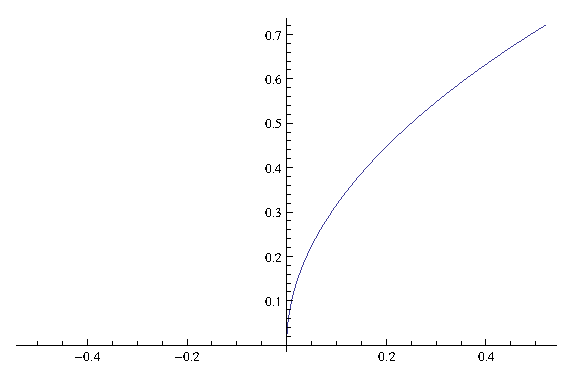
\includegraphics[width=0.3\textwidth]{continuous/functions/sqrtx}
    }
    \subfigure[A plot of $f^{-1}(\sqrt x)=x^2$.]{\
      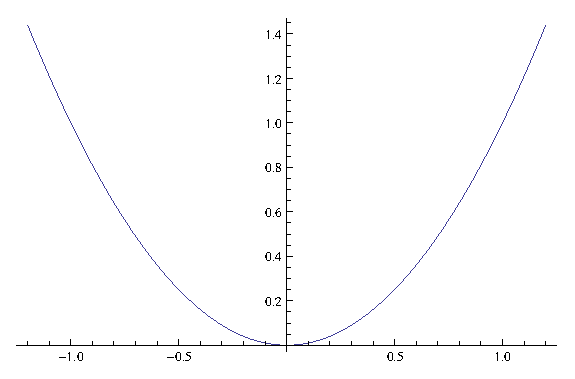
\includegraphics[width=0.3\textwidth]{continuous/functions/x2inv}
    }
  \end{center}
  \label{fig:inversef}
\end{figure}
\begin{remark} \index{composition}\index{inverse functions}
  By definition, either composite of a function and its inverse will return the 
  identity function, where $y=x$. For example:
  \[ (f \circ f^{-1})(x)=f(f^{-1}(x))=x, \]
  or
  \[ (f^{-1} \circ f)(x)=f^{-1}(f(x))=x. \]
\end{remark}

\subsection{Finding Inverse Functions}
To find the inverse of a function $f(x)$, replace $f(x)$ with $y$ and solve for 
$x$ in terms of $y$. Then, interchange $x$ and $y$.
\begin{ex}
  \label{ex:inverses}
  Find the inverse of $y=\frac{1}{2}x+1$, expressed as a function of $x$.
  \begin{sol}
    First, we solve the function for $x$ in terms of $y$.
    \begin{align*}
      y &= \frac{1}{2}x+1 \\
      \intertext{Multiply both sides by $2$.}
      2y &= x + 2 \\
      \intertext{Now subtract $2$ from both sides, and swap the left and right 
          sides of the equation.}
      x &= 2y -2
      \intertext{Now we swap $x$ and $y$.}
      y &=2x-2
    \end{align*}
    The inverse of the function $f(x)=\frac{1}{2}x+1$ is the function 
    $f^{-1}(x)=2x-2$.
    \begin{figure}[H]
      \begin{center}
        \subfigure[A plot of $f(x)=\frac{1}{2}x+1$.]{\
          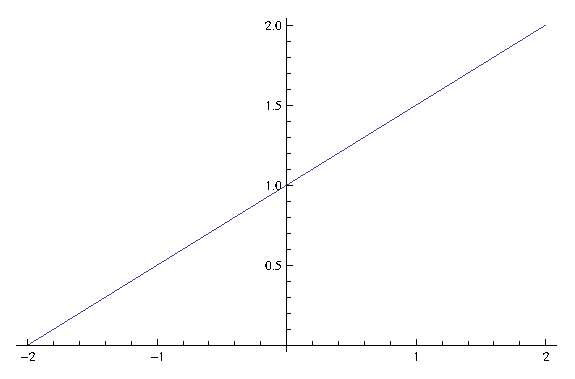
\includegraphics[width=0.45\textwidth]{continuous/functions/halfxeg}
        }
        \subfigure[A plot of $f^{-1}(x)=2x-2$.]{\
          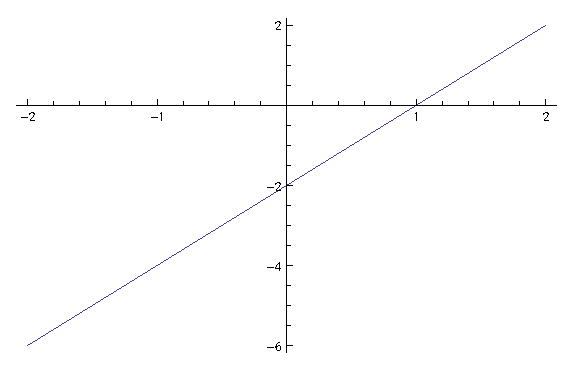
\includegraphics[width=0.45\textwidth]{continuous/functions/halfxeginv}
        }
      \end{center}
      \caption{Plots of functions from Example~\ref{ex:inverses}.}
      \label{fig:inverseg}
    \end{figure}
  \end{sol}
\end{ex}

\chapter{Trigonometry}


\section{Trigonometric Identities}\index{trigonometric identities}
\begin{figure}[h]
  \begin{center}
      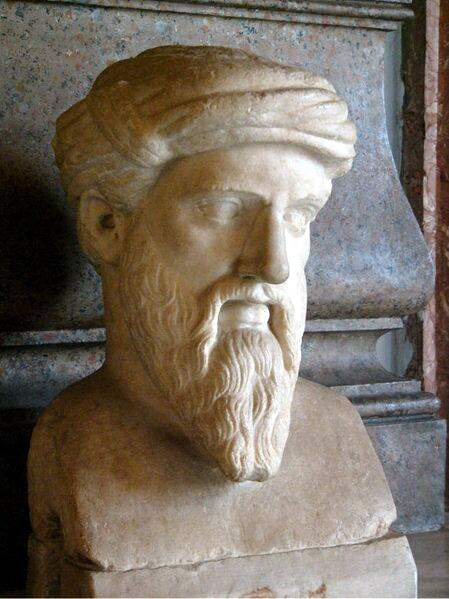
\includegraphics[width=0.7\textwidth]{photos/pythagoras.jpg}
    \end{center}
    \caption{/emph{Busto di Pitagora. Copia romana di originale greco. Musei Capitolini, Roma}.
    Original uploader was \emph{Galilea} at \url{http://de.wikipedia.org}.
    File used under the terms of the Creative Commons Attribution-Share Alike 3.0 Unported license.}
  \label{fig:bustofpythagoras}
\end{figure}
\begin{figure}[h]
  \begin{tikzpicture}[scale=5.3,cap=round,>=latex]
  % draw the coordinates
    \draw[->] (-1.5cm,0cm) -- (1.5cm,0cm) node[right,fill=white] {$x$};
    \draw[->] (0cm,-1.5cm) -- (0cm,1.5cm) node[above,fill=white] {$y$};

  % draw the unit circle
    \draw[thick] (0cm,0cm) circle(1cm);

    \foreach \x in {0,30,...,360} {
          % lines from center to point
      \draw[gray] (0cm,0cm) -- (\x:1cm);
          % dots at each point
      \filldraw[black] (\x:1cm) circle(0.4pt);
          % draw each angle in degrees
      \draw (\x:0.6cm) node[fill=white] {$\x^\circ$};
    }

  % draw each angle in radians
    \foreach \x/\xtext in {
      30/\frac{\pi}{6},
      45/\frac{\pi}{4},
      60/\frac{\pi}{3},
      90/\frac{\pi}{2},
      120/\frac{2\pi}{3},
      135/\frac{3\pi}{4},
      150/\frac{5\pi}{6},
      180/\pi,
      210/\frac{7\pi}{6},
      225/\frac{5\pi}{4},
      240/\frac{4\pi}{3},
      270/\frac{3\pi}{2},
      300/\frac{5\pi}{3},
      315/\frac{7\pi}{4},
      330/\frac{11\pi}{6},
    360/2\pi}
    \draw (\x:0.85cm) node[fill=white] {$\xtext$};

    \foreach \x/\xtext/\y in {
      % the coordinates for the first quadrant
      30/\frac{\sqrt{3}}{2}/\frac{1}{2},
      45/\frac{\sqrt{2}}{2}/\frac{\sqrt{2}}{2},
      60/\frac{1}{2}/\frac{\sqrt{3}}{2},
      % the coordinates for the second quadrant
      150/-\frac{\sqrt{3}}{2}/\frac{1}{2},
      135/-\frac{\sqrt{2}}{2}/\frac{\sqrt{2}}{2},
      120/-\frac{1}{2}/\frac{\sqrt{3}}{2},
      % the coordinate on s for the third quadrant
      210/-\frac{\sqrt{3}}{2}/-\frac{1}{2},
      225/-\frac{\sqrt{2}}{2}/-\frac{\sqrt{2}}{2},
      240/-\frac{1}{2}/-\frac{\sqrt{3}}{2},
      % the coordinates for the fourth quadrant
      330/\frac{\sqrt{3}}{2}/-\frac{1}{2},
      315/\frac{\sqrt{2}}{2}/-\frac{\sqrt{2}}{2},
      300/\frac{1}{2}/-\frac{\sqrt{3}}{2}}
      \draw (\x:1.25cm) node[fill=white] {$\left(\xtext,\y\right)$};

  % draw the horizontal and vertical coordinates
  % the placement is better this way
      \draw (-1.25cm,0cm) node[above=1pt] {$(-1,0)$}
      (1.25cm,0cm)  node[above=1pt] {$(1,0)$}
      (0cm,-1.25cm) node[fill=white] {$(0,-1)$}
      (0cm,1.25cm)  node[fill=white] {$(0,1)$};
  \end{tikzpicture}
  \caption{The unit circle.\cite{tikzunitcirc}\label{fig:tikzunitcirc}}
\end{figure}

Our first pythagorean identity is just derived from the pythagorean theorem.
\begin{figure}[H]
  \begin{center}
    \subfigure[The Pythagorean Theorem states that the sum of the areas square $a$ and square $b$ is equal to the area of square $c$.]{
      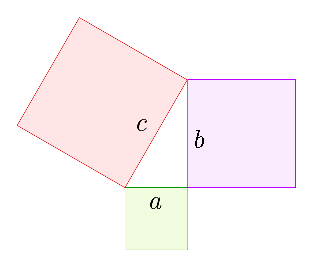
\includegraphics{continuous/functions/pyth.eps}
      \label{fig:pyth}
    }
    \hspace{0.1\textwidth}
    \subfigure[The equation for a unit circle is $a^2+b^2=1$. This creates a circle with a radius of $1$.]{
      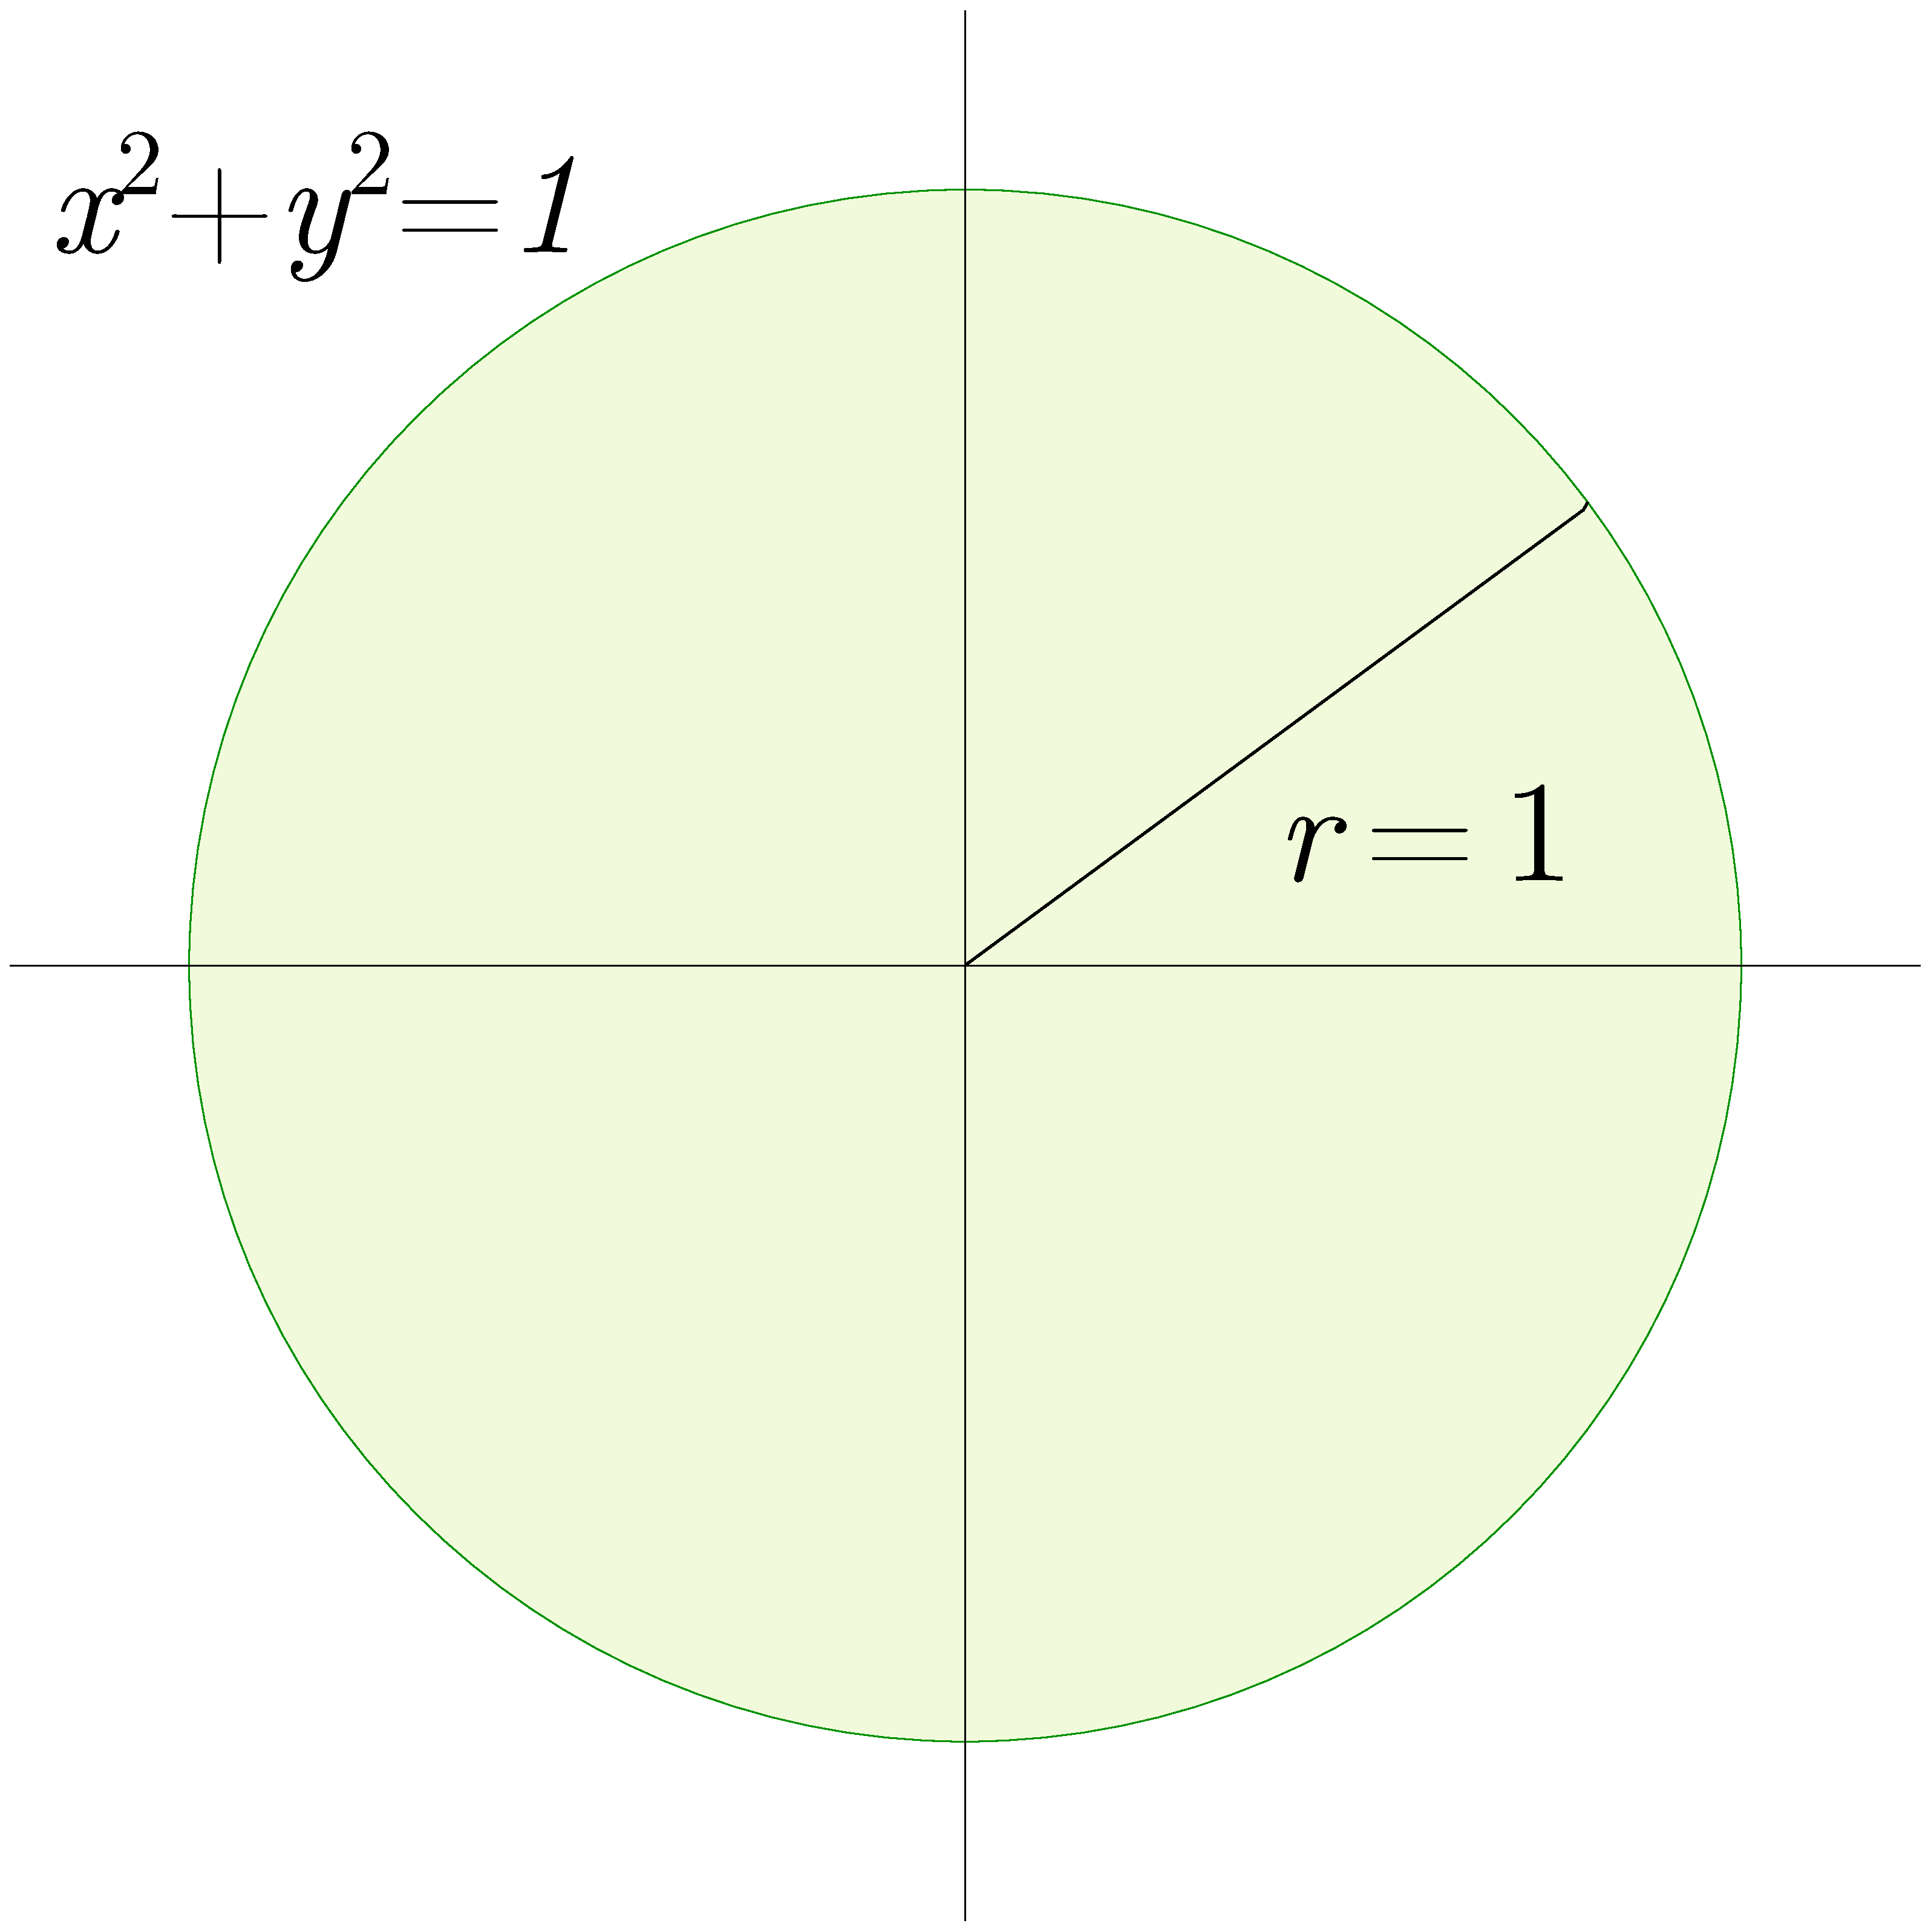
\includegraphics[width=0.3\textwidth]{continuous/functions/unitcirc.eps}
      \label{fig:basicuniticircle}
    }
  \end{center}
\end{figure}
\begin{equation}
  \sin^2x+\cos^2x=1
  \label{eq:pythtrig}
\end{equation}
\begin{figure}[H]
  \begin{center}
    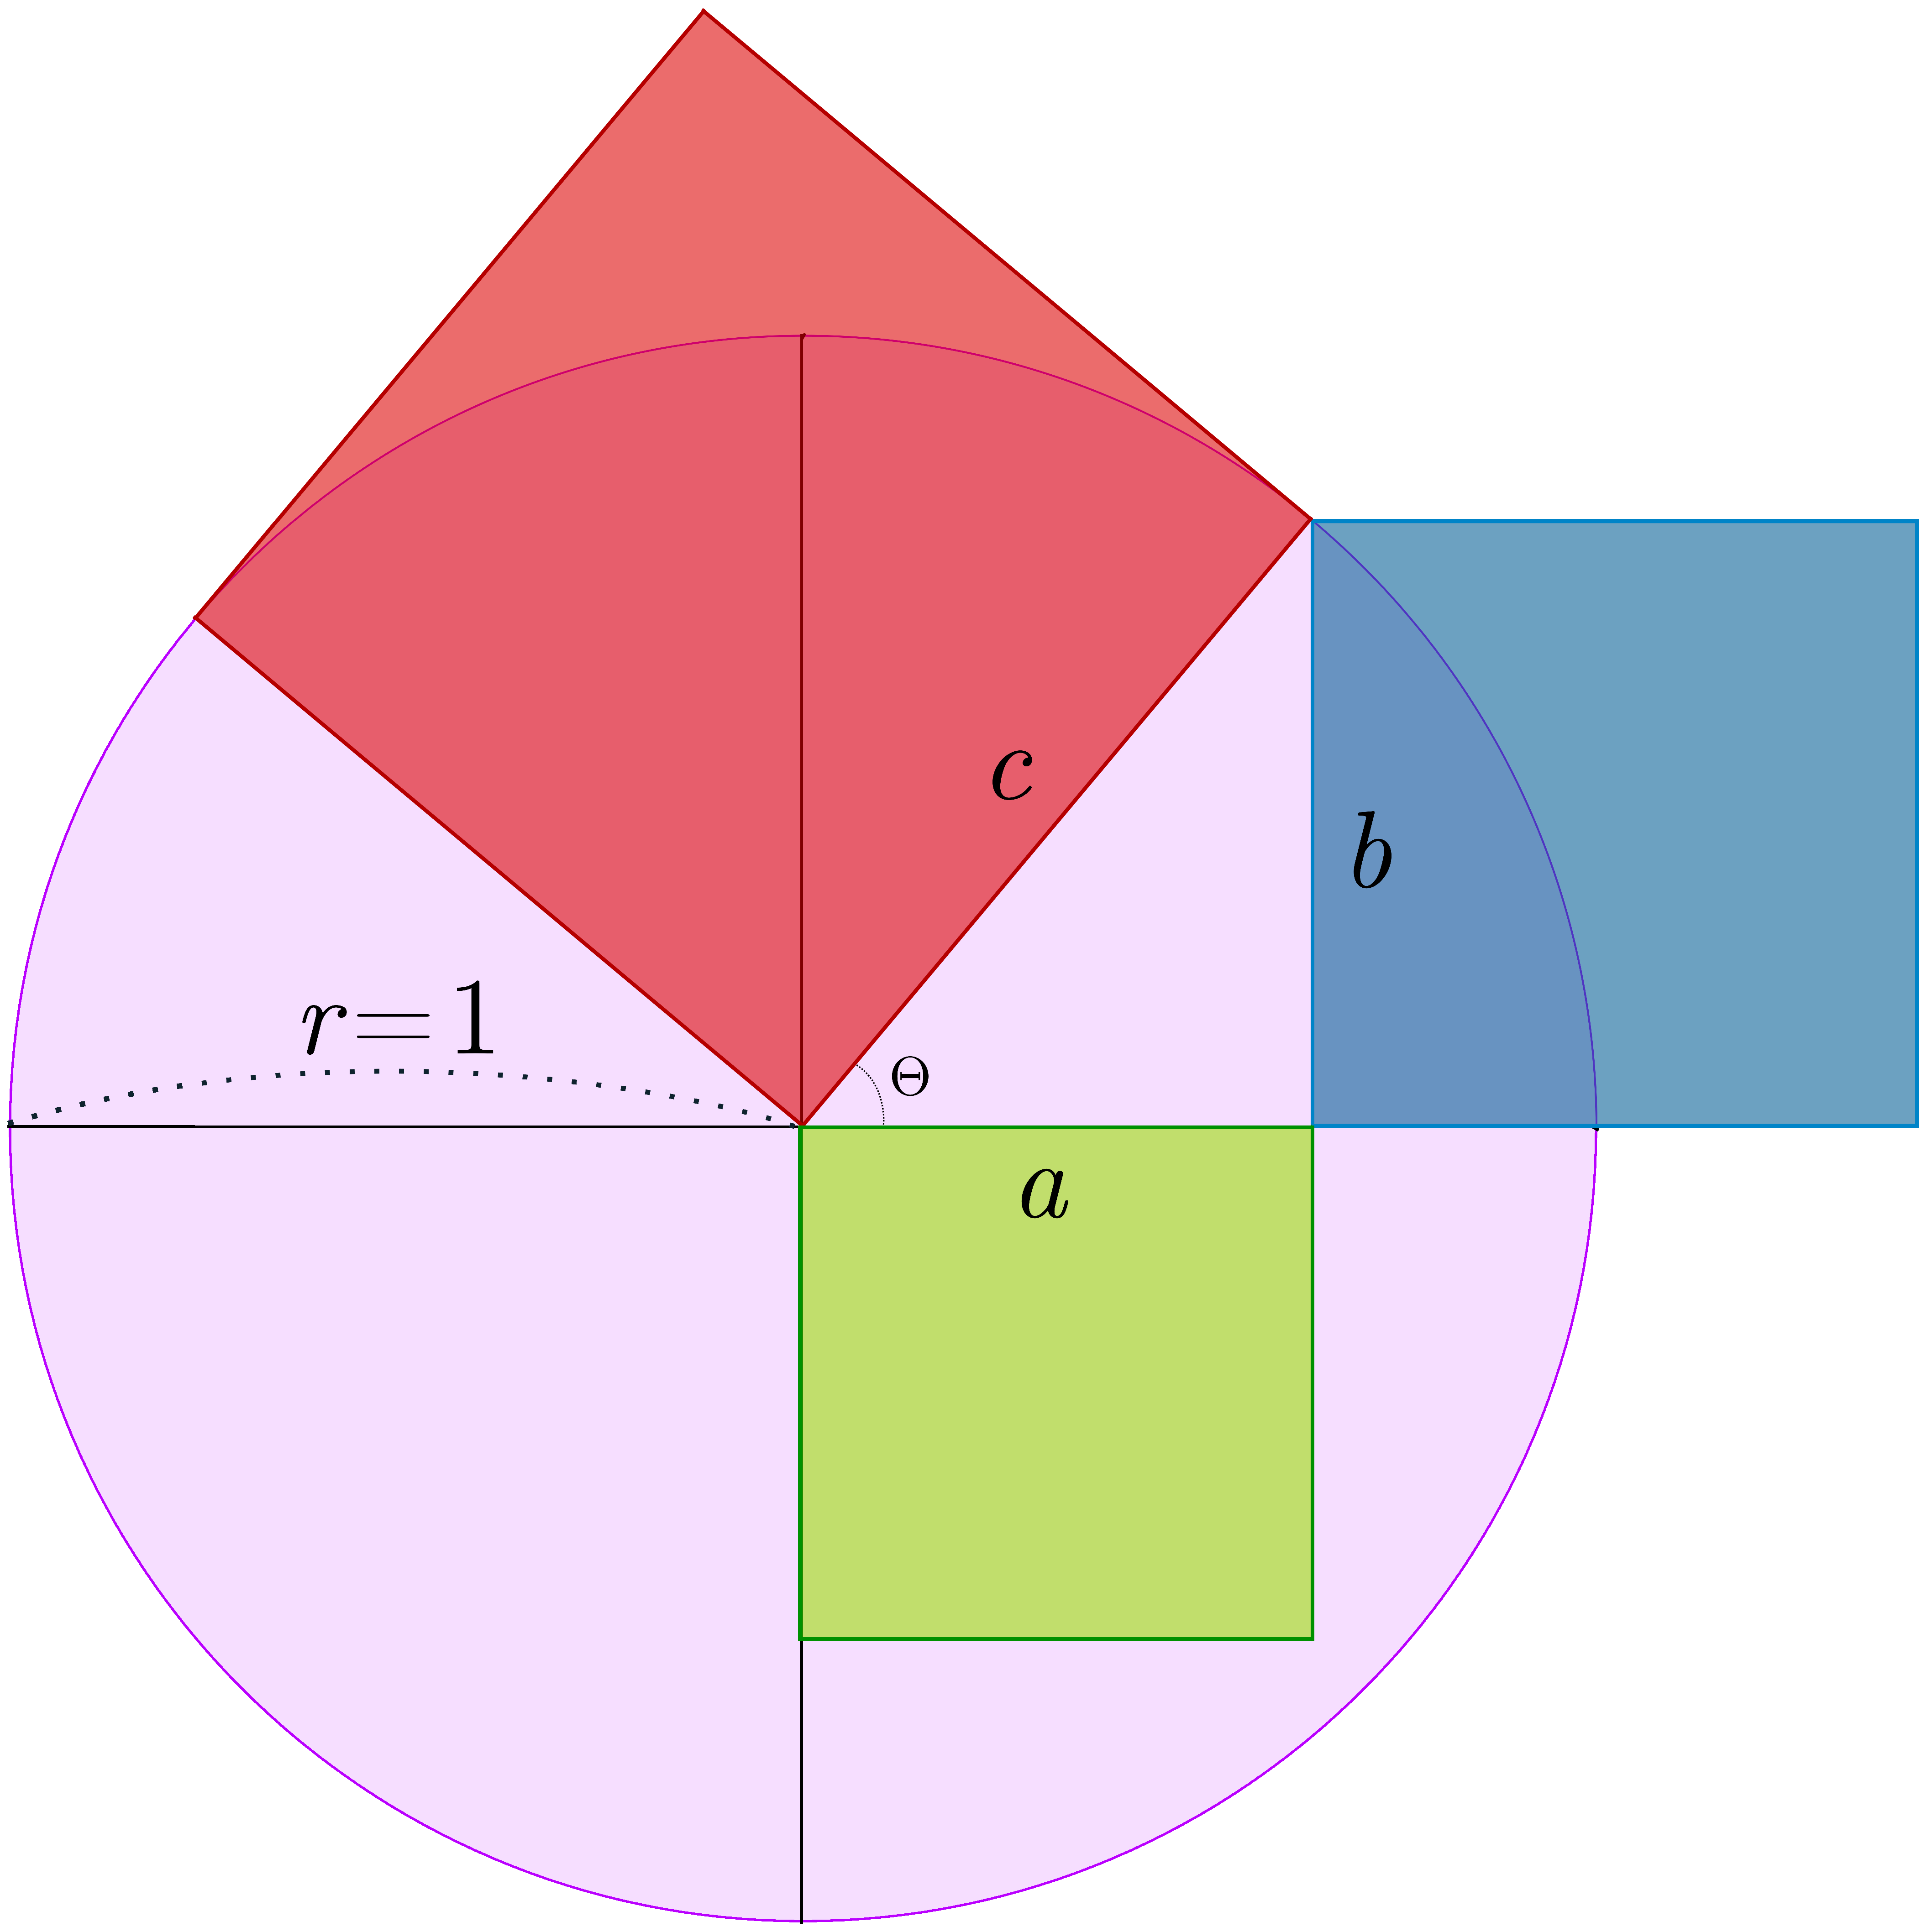
\includegraphics[width=0.3\textwidth]{continuous/trig/pythcircle.eps}
    \caption{The pythagorean squares on a unit circle.}
  \end{center}
  \label{fig:pythcircle}
\end{figure}
Because the radius of the circle is $1$, then the length of side $c$ must also equal $1$.
From this, we can conclude that $\sin^2x+\cos^2x$ must, indeed, equal 1.

To make sure we understand this on a geometric level, let's first go over the basic trigonometric functions and their relationship with our triangle.
\begin{figure}[H]
  \begin{center}
    
\includegraphics[width=0.3\textwidth]{continuous/trig/basictrig.eps}
  \end{center}
\end{figure}
For this example:
\begin{itemize}
  \item $\sin\theta=b/c$
  \item $\cos\theta=a/c$
  \item $\tan\theta=b/a$
\end{itemize}
Gennerally speaking, for an angle $\theta$ on the inside of a triangle,
\begin{itemize}
  \item$\sin\theta$ is equal to the \emph{length of the opposite side divided by the length of the hypotenuse}.
  \item$\cos\theta$ is equal to the \emph{adjacent side divided by the hypotenuse}.
  \item$\tan\theta$ is equal to the \emph{opposite over the adjacent side}.
\end{itemize}

The other ones, we either have to memorize or learn to derive (described in Section \ref{sec:trigderiv}).
\begin{equation}
  \sin{(x+y)} = \sin x \cos y + \sin y \cos x
\end{equation}
\begin{equation}
  \sin{(x-y)} = \sin x \cos y - \sin y \cos x
\end{equation}
\begin{equation}
  \cos(x+y)=\cos x \cos y - \sin x \sin y
  \label{eq:cosxpy}
\end{equation}
\begin{equation}
  \cos(x-y)=\cos x \cos y + \sin x \sin y
\end{equation}
\begin{equation}
  \sin{-x}=-\sin x
\end{equation}
\begin{equation}
  \sin{-x}=-\sin x
\end{equation}
\begin{equation}
  \sin{2x}=2 \big( \sin x \cos x \big)
\end{equation}
\begin{equation}
  \cos{2x}=\cos^2x-\sin^2x
\end{equation}

\subsection{Deriving Trigonometric Identities}\index{deriving trigonometric identities}\label{sec:trigderiv}

Using the pythagorean theorem and a triangle with a hypotenuse of length $1$, we can obtain our first trigonometric identity:
\begin{equation}
	\sin^2x+\cos^2x=1
  \label{eq:pyth}
\end{equation}
Dividing by $\sin^2x$ gives us:
\begin{align}
\frac{\sin^2x}{\sin^2x}+\frac{\cos^2x}{\sin^2x}&=\frac{1}{\sin^2x} \nonumber \\
	1+\cot^2x&=\csc^2x
\end{align}
Dividing by $\cos^2x$ produces:
\begin{align}
  \frac{\sin^2x}{\cos^2x}+\frac{\cos^2x}{\cos^2x}+=&\frac{1}{\cos^2x} \nonumber \\
	\tan^2x+1=&\sec^2x
\end{align}

We should also memorize the following two identities:
\begin{equation}
  \sin{a+b}=\sin a \cos a + \sin b \cos b
  \label{eq:sinab}
\end{equation}
\begin{equation}
  \cos{a+b}=\cos a \cos b + \sin a \sin b
  \label{eq:cosab}
\end{equation}
From equation \eqref{eq:sinab} we can infer that
\begin{equation}
  \sin{2\theta}=2 \sin \theta \cos \theta
  \label{eq:sin2q}
\end{equation}
and from equation \eqref{eq:cosab} we can infer that
\begin{equation}
  \cos{2\theta}=\cos^2 \theta - \sin^2\theta
  \label{eq:cos2q}
\end{equation}

By rearranging \eqref{eq:cos2q} and substituting from \eqref{eq:pyth} we can derive power reduction identities for $\cos^2 \theta$
\begin{align}
  \cos{2\theta} &= \cos^2 \theta - \sin^2\theta \nonumber \\
  \cos{2\theta} + \sin^2\theta &= \cos^2\theta \nonumber \\
  \cos{2\theta} + (1-\cos^2 \theta) &=\cos^2\theta \nonumber \\
  \cos{2\theta} + 1 &= \cos^2\theta + \cos^2\theta \nonumber \\
  \cos{2\theta}+1 &= 2 \cos^2\theta \nonumber \\
  \cos^2\theta &= \frac{\cos{2\theta}+1}{2}
  \label{eq:cossqq}
\end{align}
and for $\sin^2 \theta$
\begin{align}
  \cos{2\theta} &= \cos^2 \theta - \sin^2\theta \nonumber \\
  \sin^2 \theta &= \cos^2 \theta - \cos{2 \theta} \nonumber \\
  \sin^2 \theta &= (1-\sin^2 \theta) - \cos{2 \theta} \nonumber \\
  2 \sin^2 \theta &= 1-\cos{2\theta} \nonumber \\
  \sin^2 \theta &= \frac{1-\cos{2\theta}}{2}
  \label{eq:sinsqq}
\end{align}


\subsection{Examples}

\begin{ex}
  Find the value of
  \[ \cos{\frac{11 \pi}{12}} \text{.}\]
  \begin{sol}
    We first rewrite the problem to fit one of our trigonometric identities,
    then use equation \eqref{eq:cosxpy} to break apart \(\cos{\frac{11 \pi}{12}}\).
    \begin{align*}
      \cos{\frac{11 \pi}{12}}
      =&\cos{\frac{\pi}{4}+\frac{2 \pi}{3}}
      =\cos{\frac{\pi}{4}} \cos{\frac{2\pi}{3}}
        -\sin\frac{\pi}{4} \sin\frac{2\pi}{3} \\
      \intertext{Unlike in the original problem, we can easily simplify our new expression.}
      \cos{\frac{\pi}{4}} \cos{\frac{2\pi}{3}}
        - \sin{\frac{\pi}{4}} \sin{\frac{2\pi}{3}}
      =& \frac{\sqrt 2}{2} \frac{-1}{2}
        -\frac{\sqrt 2}{2} \frac{\sqrt 3}{2}
      =\frac{-\sqrt 2}{4}
        - \frac{\sqrt{6}}{4} \\
      = &\frac{-\sqrt 2}{4}(1+\sqrt 3)
    \end{align*}
  \end{sol}
\end{ex}
\begin{ex}
  Prove the following trigonometric identity:
  \[ \frac{1-\cos x}{\sin x}=\frac{\sin x}{1+\cos x} \]
  \begin{proof}
    We first cross-multiply:
    \begin{align*}
      \ (1-\cos x)(1+\cos x) &= sin^2 x \\
      \intertext{then, using equation \eqref{eq:pythtrig}, we realize that we can replace \(\sin^2 x\) with \(1-\cos^2 x\).}
       (1-\cos x)(1+\cos x) &= 1-\cos^2x\\
      \intertext{Now we simplify.}
      1-\cos x + \cos x -\cos^2 &= 1-\cos^2x \\
      1-\cos^2x &= 1-\cos^2x \qedhere
    \end{align*}
  \end{proof}
\end{ex}



\chapter{Limits}\label{limits} \index{limits}
\section{Understanding Limits}
If we have a function \(f\), defined such that
\begin{equation}
  f(x)=\frac{x^2-1}{x-1} \qquad (x \neq 1)
  \label{eq:firstlimit}
\end{equation}
this function is not defined at \(x=1\), so we cannot directly discuss its behavior at \(x=1\).
\begin{figure}[h]
  \begin{center}
    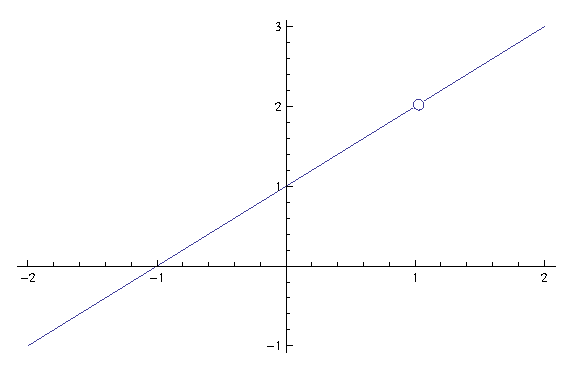
\includegraphics[scale=0.7]{graphs/p1ch3x2m1xm1}
  \end{center}
  \caption{A plot of \(f\). Note the hole at \(x=1\).}
\end{figure}
However, we may still wish to know how the function behaves \emph{around} \(x=1\).
This is where limits come in handy.
They discuss the behavior of a function near a specific point, without any consideration for how the function behaves exactly \emph{at} that point.
To find the behavior of \(f\) around \(x=1\), we take the limit of \(f\) as \(x\) approaches \(1\).
\begin{defn}\label{defn:limi}\index{limit definition}
  \( \lim_{x \to a} f(x) = L \) if and only if \(f(x)\) gets \emph{arbitrarily} close to \( L \) as \(x\) gets \emph{sufficiently} close to \(a\).
\end{defn}
\begin{remark}
  In this case, \textbf{arbitrarily close} implies that we can make the number as close as we could possibly request it. \textbf{sufficiently close} means that we can find a number $x$ where, for every number after (or before) it, we are past our arbitrary value of closeness.
\end{remark}
We would write this as:
\[ \lim_{x \to 1} \frac{x^2-1}{x-1} \]
In this case, we can evaluate this using basic algebra to simplify the original function,
\begin{align*}
   f(x)&=\frac{x^2-1}{x-1} && x \neq 1 \\
   &=\frac{(x+1)(x-1)}{x-1}&& x \neq 1 \\
   &=x+1 && x \neq 1
\end{align*}
\begin{remark}
  We must make the statement that $x \neq 1$ whenever $x+1$ is in the denominator of a function,
  because if $x$ could ever be equal to $1$, it would make the value of $f(x)$ undefined at this point.
\end{remark}
Then we define a new function equivalent to the above, but where \(1 \in D\).
We then evaluate our new function at \(x=1\).
\[ g(x) = x+1 \]
Which gives us
\begin{align*}
  \lim_{x \to 1} \frac{x^2-1}{x-1}
  &=g(1)
  \\&=2
  \text{.}
\end{align*}

It turns out we have a number of rules that describe how we can go about
evaluating a limit.
\begin{theorem}[Limit Laws]
  If \(L\), \(M\), and \(k\) are real numbers and
    \[ \lim_{x \to c} f(x)=L \quad and \lim_{x \to c} g(x) = M \]
  then,
  \begin{table}[H]
    \centering
      \begin{tabular}{p{3in}>\(p{3in}<\)}
        Sum Rule: & \displaystyle{\lim_{x \to c} (f(x) + g(x)) = L + M} \\ \\
        Difference Rule: & \displaystyle{\lim_{x \to c} (f(x) - g(x))=L-M} \\ \\
        Constant Multiple Rule: & \displaystyle{\lim_{x \to c} (k \cdot f(x)) = k
      \cdot L} \\ \\
      Quotient Rule: & \displaystyle{\lim_{x \to c} \frac{f(x)}{g(x)} =
      \frac{L}{M}, \quad m\neq 0} \\ \\
      Power Rule: & \displaystyle{\lim_{x \to c} [f(x)]^n = L^n, \quad n \in
      \mathbf{Z_+}} \\ \\
      Root Rule: & \displaystyle{\lim_{x \to c} \sqrt[n]{f(x)} =
      \sqrt[n]{L}=L^{1/n}, \quad n
    \in Z_+}
  \end{tabular}
  \end{table}
  If \(n\) is even, we assume that \(\lim_{x \to c} f(x) = L > 0\). This is because for the rules including exponents, for $\lim{x\to c} f(x)=L<0$ to be true we would require imaginary numbers.
\end{theorem}

Not all functions have limits defined everywhere on their domain.
For example, \(h(x)=\sin \frac{1}{x} \) oscillates indefinitely as \(x \to 0\), as shown in Figure \ref{fig:p1sin1x}.
\begin{figure}[H]
  \begin{center}
    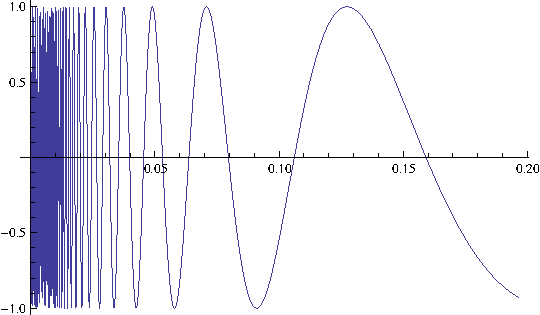
\includegraphics{graphs/p1sin1x.pdf}
  \end{center}
  \caption{The limit of \(h(x)\) as \(x \to 0\) does not exist.}
  \label{fig:p1sin1x}
\end{figure}
As \(x\to0\), it is impossible to say whether \(f(x)\) is approaching \(1\) or \(-1\).
This is an example of an \textbf{oscillating discontinuity}\index{oscillating discontinuity}.
There are more situations in which a limit does not exist.

In a \textbf{infinite discontinuity}\index{infinite discontinuity}, the graph jumps to $\infty$ or $-\infty$ at certain $x-values$.
No limit can exist here.
\begin{figure}[H]
  \begin{center}
    \includegraphics[width=0.4\textwidth]{continuous/limits/infinited}
  \end{center}
  \caption{An infinite discontinuity at $x=0$.}
\end{figure}

The other situation which can cause a limit to not exist at a point is a \textbf{jump discontinuity}\index{jump discontinuity}.
\begin{figure}[H]
  \begin{center}
    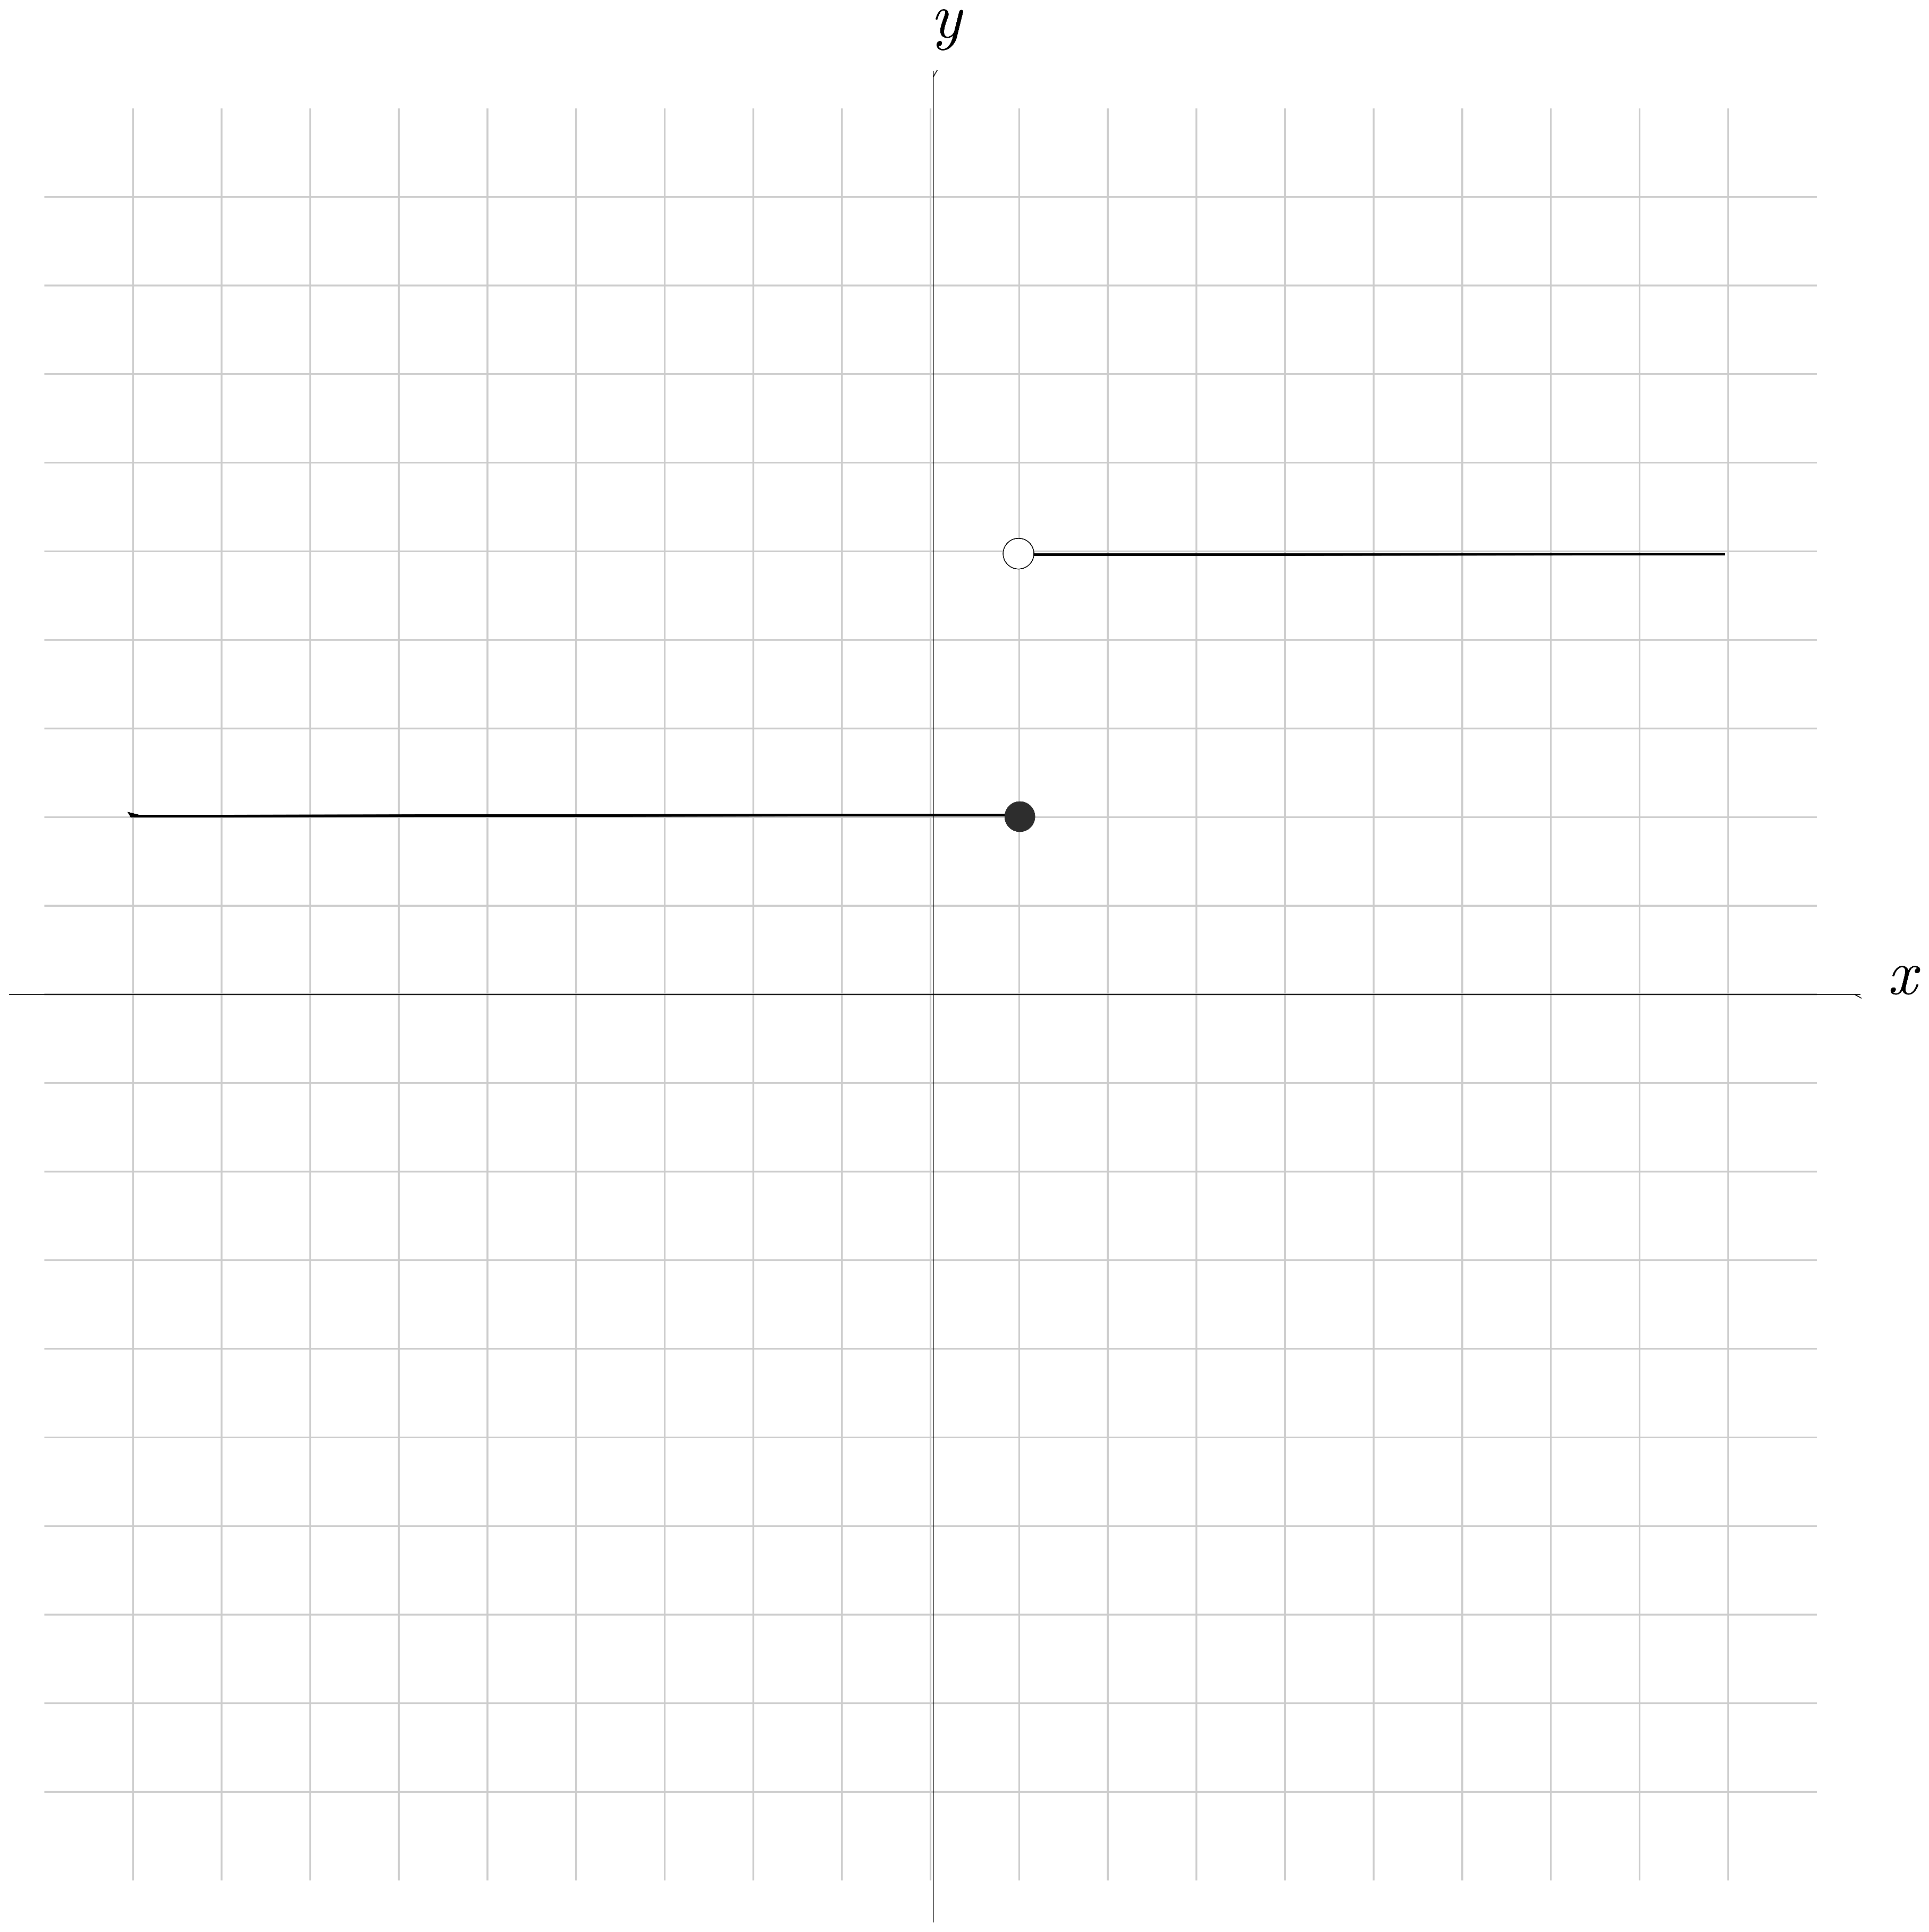
\includegraphics[width=0.3\textwidth]{continuous/limits/jumps}
  \end{center}
  \caption{A jump discontinuity.}
\end{figure}
\subsection{Side Limits}\index{side limits}

In places where a limit does not exist, we can still talk about the limit from just one side or another.
Note, however, that if $\lim_{x\to a}f(x)$ at a point, then the left an right limits also exist and must be equal to one another.

\begin{theorem}
  \( \lim_{x\to a^-} f(x)=L \) iff \(f(x)\) gets arbitrarily close to \(L\) as \(x\) comes sufficiently close to \(a\), but \(x < a \).
  \label{theorem:lefthandlimit}
\end{theorem}
\begin{figure}[H]
  \begin{center}
    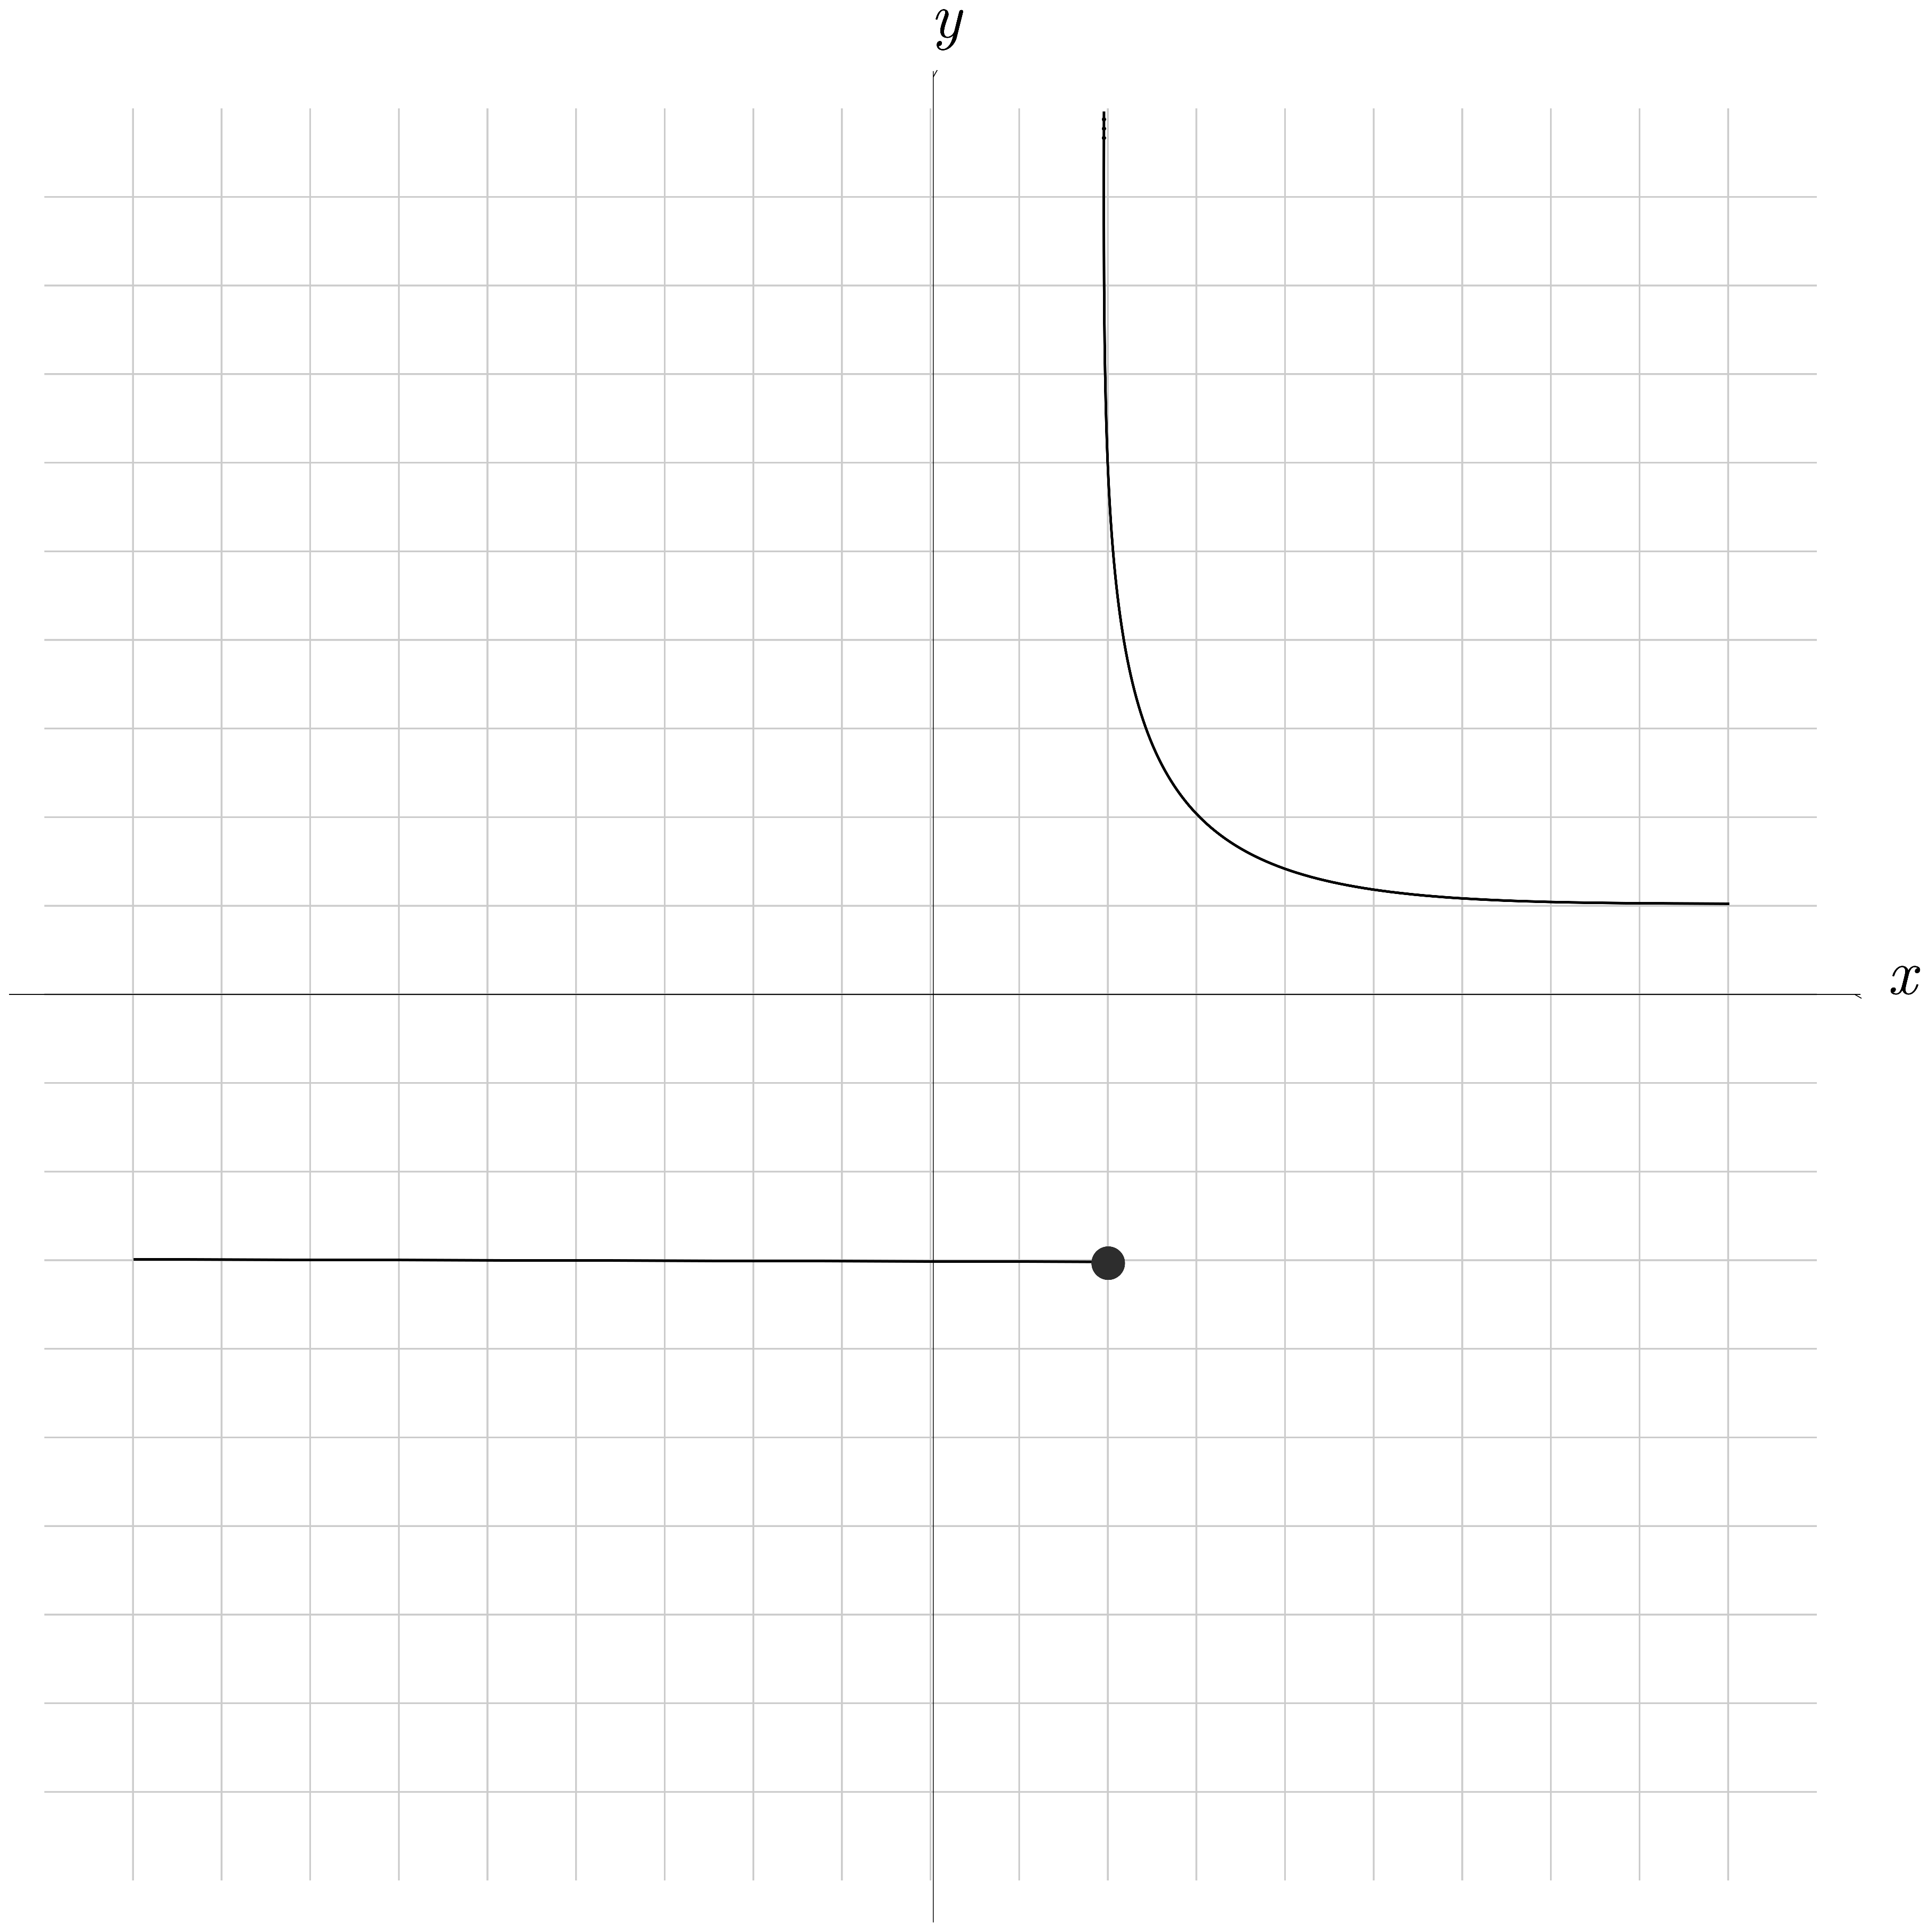
\includegraphics[width=0.5\textwidth]{continuous/limits/llmt}
  \end{center}
  \caption{The lefthand limit at $x=2$ exists, though the righthand limit does not.}
\end{figure}
\begin{theorem}
  \( lim_{x \to a^+} f(x)=L \) iff \(f(x)\) gets arbitrarily close to \(L\) as \(x\) gets sufficiently close to \(a\), but \(x > a\).
  \label{}
\end{theorem}
% section ref: Thomas' Calculus, Chapter 1

\subsection{The Sandwich Theorem}

Let us look at a more complicated example of a limit.
Suppose we have the functions
\begin{align*}
  h(x) &= |x|, \\
  f(x) &= x\sin{\frac{1}{x}}, \\
  \text{and }g(x) &= -|x|,
\end{align*}
where at \(x=0\), \(g(x) \leq f(x) \leq h(x)\) at 0.
\begin{figure}[H]
  \begin{center}
    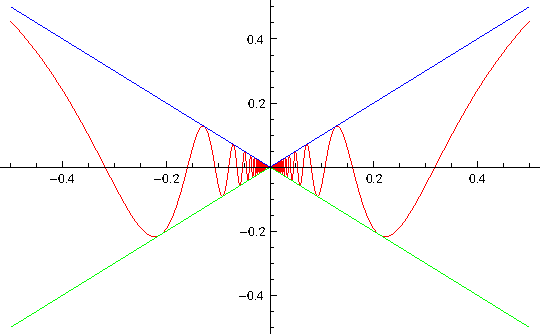
\includegraphics{graphs/sandwichtheorem.pdf}
  \end{center}
  \caption{A plot of \(h(x)\), \(f(x)\), and \(g(x)\)}
\end{figure}
We can conclude, intuitively, that the limit of \(f(x)\) as \(x \to 0\) must be
0 even though we cannot evaluate \(f(x)\) at 0, as seen in Figure
\ref{fig:p1sin1x}. We can generalize this kind of behavior as a theorem, the
\emph{sandwich theorem}.
\begin{theorem}[The Sandwich Theorem]
  If \[g(x) \leq f(x) \leq h(x)\] holds for all \(x \neq c\) in some open interval containing a number \(c\),
  and
  \[ \lim_{x \to c} g(x) = \lim_{x \to c} h(x) = L, \]
  then \(\lim_{x \to c} f(x)\) also equals $L$.
  \label{th:sandwich}
  \index{sandwich theorem}
\end{theorem}

\section{\emph{Epsilon}-\emph{Delta} Definition of a Limit}\index{epsilon-delta definition of a
limit}

The statement
\[ \lim_{x \to a} f(x) = L \]
is the statement
\begin{equation}
  \forall (\varepsilon > 0) \exists (\delta>0) \forall x \Big(0 < | x -a| < \delta \implies
  \big|f(x)-L\big| < \varepsilon\Big),
  \label{eq:e_d_limit}
\end{equation}
where the domain for the variables for $\delta$ and $\varepsilon$ consists of
all positive real numbers and for $x$ consists of all real
numbers.

\section{Evaluating Limits}

Let's look at a really complicated example of a limit\footnote{Credit for this example goes to Dr. Dobrescu's Math 140 class at CNU, Spring 2011.}, to make sure we truly understand them.
For piecewise-defined functions, limits can get especially interesting. Here's an example:
\index{piecewise function}

\begin{ex}
  \[ f(x)=
    \begin{dcases}
      x &: x \in \left[ -1,0 \right) \\
      -x &: x \in \left (0,1 \right) \\
      x-1 &: x \in \left[1, 2\right]
    \end{dcases}
    \]
  \begin{figure}[h]
    \begin{center}
      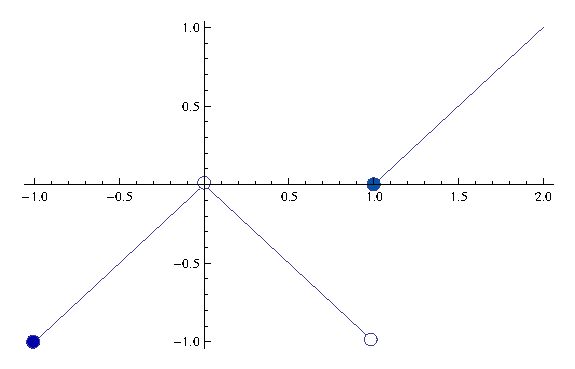
\includegraphics{graphs/pwlimex1}
    \end{center}
    \caption{A graph of \(f(x)\)}
    \label{fig:pwlimex1}
  \end{figure}
  \begin{enumerate}
    \item Does \( \lim_{x\to 0} f(x) \) exist?

      \begin{sol}
        Yes.
      \end{sol}
    \item Does \( \lim_{x \to 0} f(x)=0 \)?

      \begin{sol}
        Yes.
      \end{sol}
    \item Does \(\lim_{x \to 0} f(x)=1\)?

      \begin{sol}
        No. \(\lim_{x \to 0} f(x)=0\).
      \end{sol}
    \item Does \(\lim_{x \to 1} f(x)=1\)?

      \begin{sol}
        No. \( \lim_{x \to 1} f(x) \) does not exist.
      \end{sol}
    \item Does \(\lim_{x \to 1} f(x)=0\)?

      \begin{sol}
        No. The limit does not exist.
      \end{sol}
    \item Can we take \( \lim_{x \to x_0} f(x)\) for every \(\big(x_0 \in (-1, 1)\big)\)?

      \begin{sol}
        Yes.
      \end{sol}
    \item Does \( \lim_{x \to 1} f(x) \) exist?

      \begin{sol}
        Yes.
      \end{sol}
  \end{enumerate}
\end{ex}
\begin{ex}
  Find
  \[ \lim_{x \to 4} \frac{4x-x^2}{2-\sqrt x} \text{.} \]
  \begin{sol}
    \begin{figure}[h]
      \begin{center}
        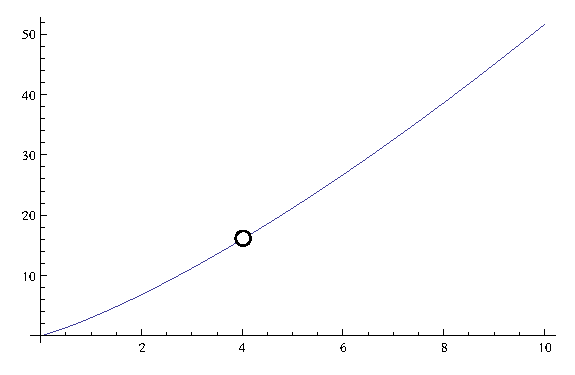
\includegraphics[width=0.4\textwidth]{continuous/limits/4xmx2}
      \end{center}
      \caption{A plot of $f(x)= \frac{4x-x^2}{2-\sqrt x}$.}
    \end{figure}
    First we multiply by the conjugate of the denominator to remove the radical from it. For more detail on conjugates, see Section \ref{app:def:conjugate}.
    \begin{align*}
      \lim_{x \to 4} \frac{4x-x^2}{2-\sqrt x}
      &= \lim_{x \to 4} \frac{4x-x^2}{2-\sqrt x} \cdot \frac{2+\sqrt x}{2+\sqrt x}\\
      \intertext{Then we simplify.}
      &=\lim_{x \to 4} \frac{x\big(4-x\big)\big(2+\sqrt{x}\big)}{4-x}
       = \lim_{x \to 4} \frac{x\big(2+\sqrt{x}\big)}{1} \\
      &= 16
    \end{align*}
  \end{sol}
\end{ex}
\begin{ex}
  Evaluate
  \[ \lim_{x \to -1} \frac{\sqrt{x^2+8}-3}{x+1} \text{.} \]
  \begin{sol}
    \begin{align*}
      \lim_{x \to -1} \frac{\sqrt{x^2+8}-3}{x+1}
      &= \lim_{x \to -1} \frac{\sqrt{x^2+8}-3}{x+1} \cdot \frac{\sqrt{x^2+8}+3}{\sqrt{x^2+8}+3}
      = \lim_{x \to -1} \frac{x^2+8-9}{(x+1)(\sqrt{x^2+8}+3} \\
      &= \lim_{x \to -1} \frac{(x-1)(x+1)}{(x+1)(\sqrt{x^2+8}+3)}
      = \lim_{x \to -1} \frac{x-1}{\sqrt{x^2+8}+3} \\
      &= \frac{-1}{3}
    \end{align*}
  \end{sol}
\end{ex}
\begin{ex}
  Suppose we wished to evaluate the limit
  \[  \lim_{\theta \to 0} \frac{\sin \theta}{5 \theta}. \]
  \begin{sol}
    Well, first we should recognize that $\sin \theta$ is not the kind of function that is growing indefinitely:
    it oscillates forever between two values, $1$ and $-1$.
    \begin{figure}[H]
      \begin{center}
        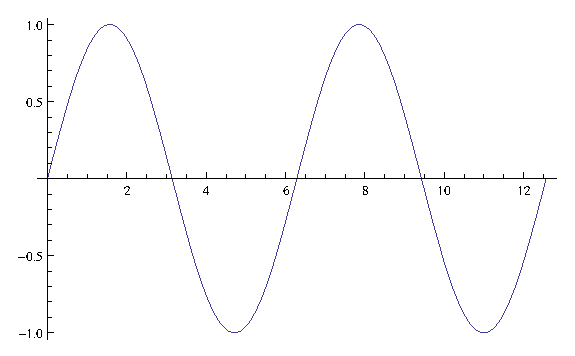
\includegraphics[width=0.5\textwidth]{continuous/limits/sintheta}
      \end{center}
      \caption{A plot of $\sin \theta$.}
      \label{fig:sintheta}
    \end{figure}
  \end{sol}
  But dividing by larger and larger values is going to make this function's \textbf{amplitude}\index{amplitude},
  its distance from the $y$-value of $0$, much smaller.

  Using Theorem \ref{th:sandwich},\footnote{How?} we can see that this limit approaches $1$.
\end{ex}

\section{Indeterminate Forms}

If we want to know how the function
$$F(x)=\frac{x-\sin x}{x^3}$$
behaves \emph{near} $x=0$ (where it is undefined), we can examine the limit of $F(x)$ as $x \to 0$. We cannot apply the Quotient Rule for limits because the limit of the denominator is $0$. Moreover, in this case, \emph{both} the numerator and denominator approach $0$, and $0/0$ is undefined. Such limits may or may not exist in general, but the limit does exist for the function $F(x)$ under discussion by applying l'Hospital's Rule, which is detailed further in Section \ref{sec:lhospital}.

If the continuous functions $f(x)$ and $g(x)$ are both zero at $x=a$, then
$$\lim_{x \to a} \frac{f(x)}{g(x)}$$
cannot be found by substituting $x=a$. The substitution produces $0/0$, a meaningless expression, which we cannot evaluate. We use $0/0$ as a notation for an expression known as an \textbf{indeterminate form}. Other meaningless expressions often occur, such as $\infty / \infty$, $\infty \cdot 0$, $\infty - \infty$, $0^0$, and $1^{\infty}$, which cannot be evaluated in a consistent way; these are called indeterminate forms as well.

\section{Continuity of Functions}
\begin{defn}
  A function is \textbf{continuous}\index{continuous} at $x=a$ iff
  \begin{itemize}
    \item $f(a)$ is defined.
    \item $\lim_{x\to a} f(x)$ exists.
    \item $\lim_{x\to a} f(x)=f(a)$.
  \end{itemize}
\end{defn}

\section{The Mean Value Theorem}
\index{mean value theorem}
The following is a simplified case of the mean value theorem:
The \textbf{mean value theorem} states that, for a continuous function $f$,
if we have an $f(a)$ which is negative and a $f(b)$ which is positive,
then $f$ crosses the $x$-axis somewhere on the interval $(a, \, b)$.

\chapter{Derivatives}

\section{Slopes}

The entire idea of a derivative is based on the idea behind the slope of a graph. You probably remember the equation for the slope of a line from algebra,
\begin{equation}
  \label{eq:slope}
  m=\frac{\Delta y}{\Delta x}=\frac{y_2-y_1}{x_2-x_1}
\end{equation}
which is usually associated with the general form of a linear equation
\begin{equation}
  y=mx+b
\end{equation}
\begin{figure}[h]
  \begin{center}
    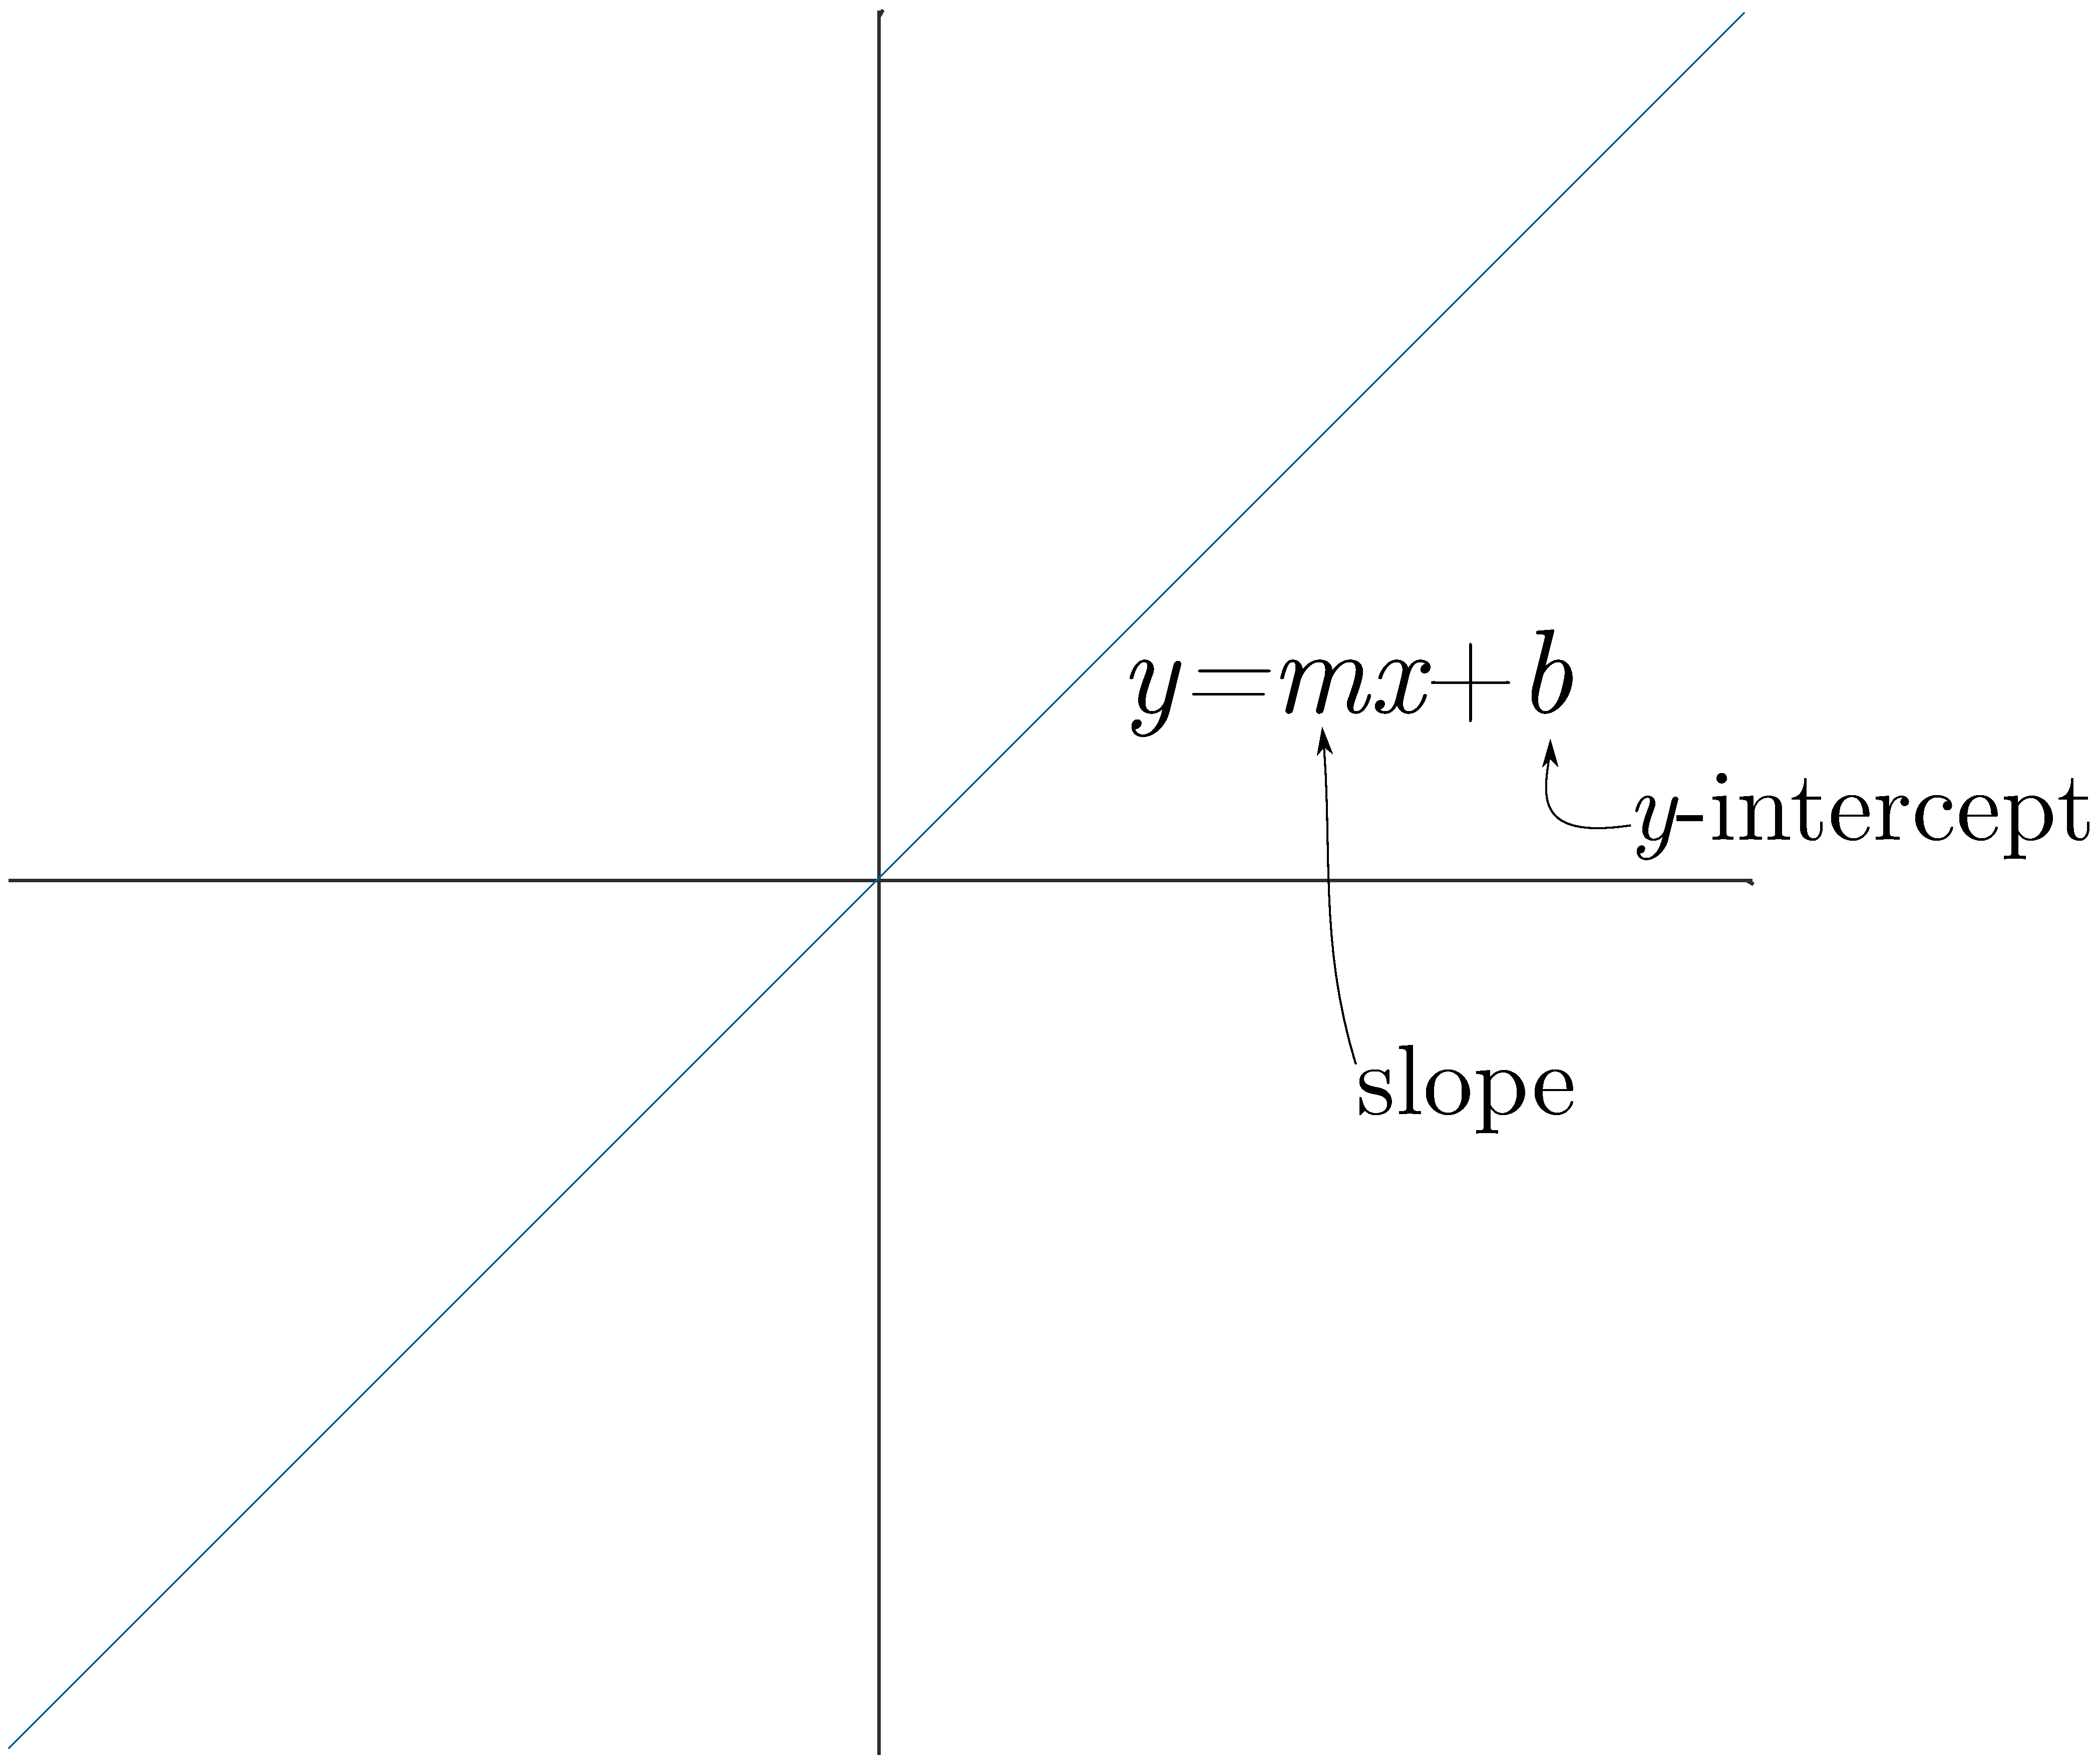
\includegraphics[width=0.5\textwidth]{continuous/derivatives/lineform.eps}
  \end{center}
  \caption{The general form equation for a line.}
\end{figure}
\begin{figure}[h]
  \begin{center}
    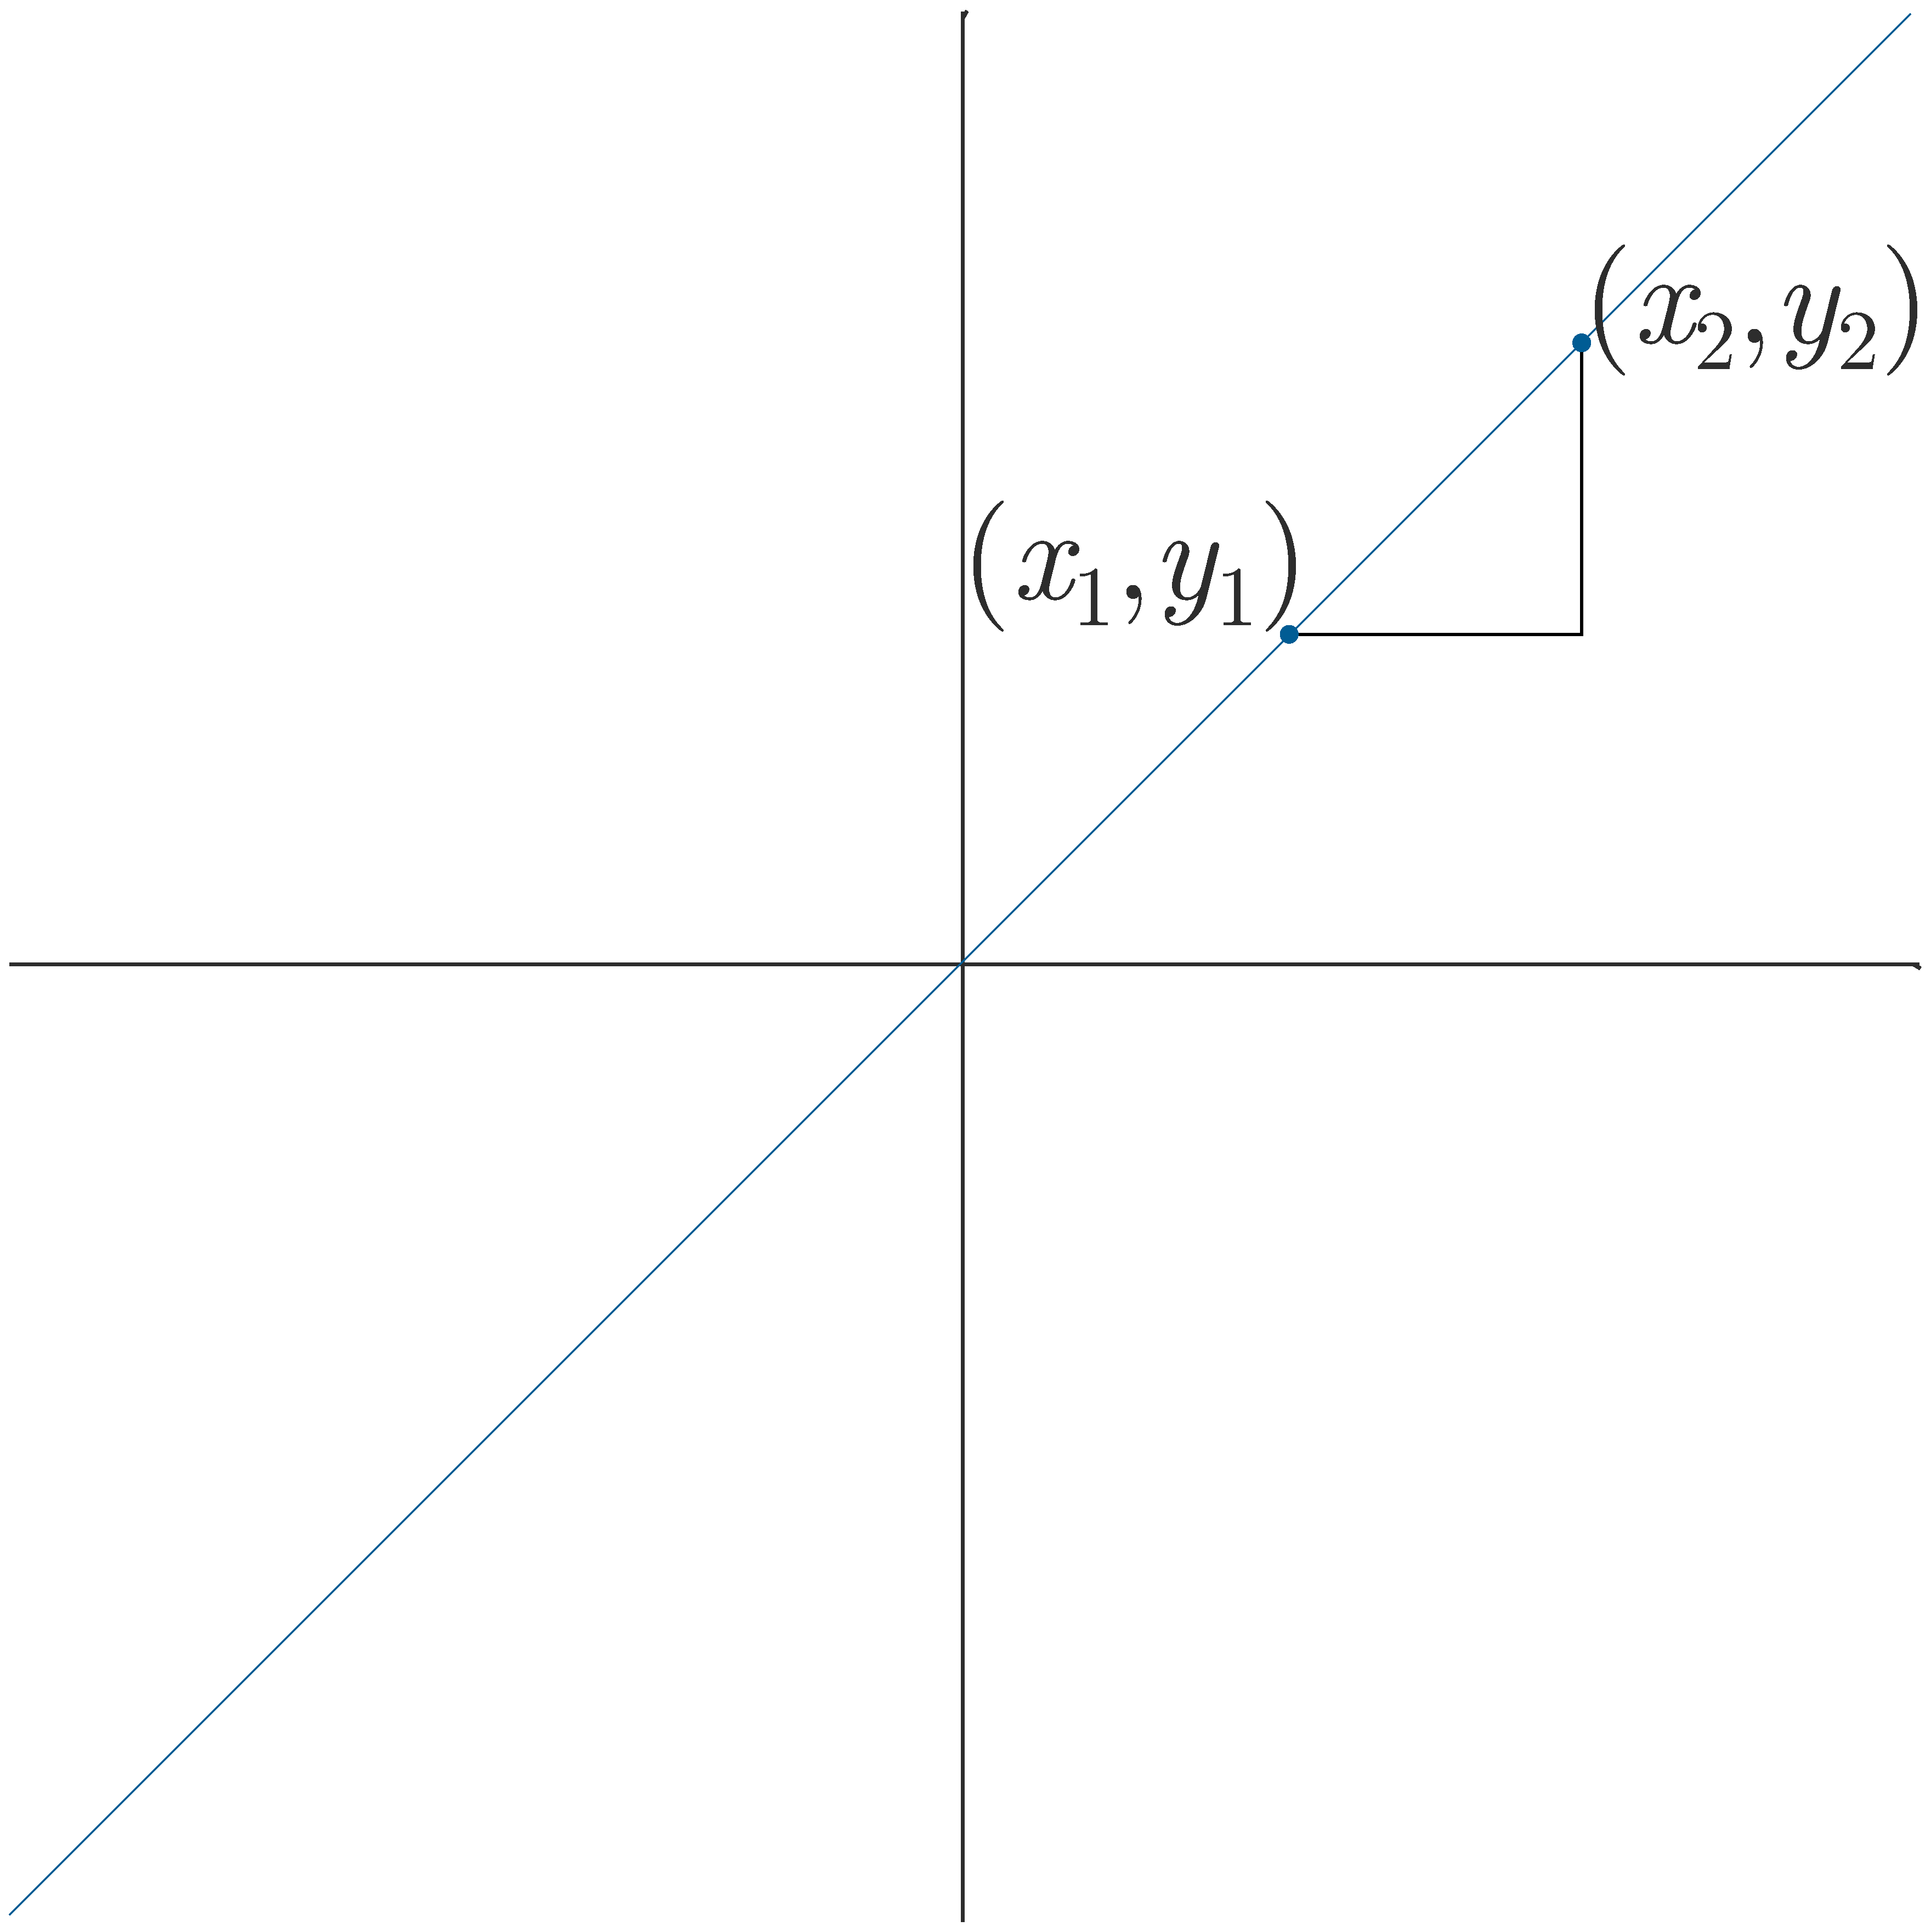
\includegraphics[width=0.5\textwidth]{continuous/derivatives/lineform_slope.eps}
  \end{center}
  \caption{How we determine ``rise over run'' in a graph.}
\end{figure}
\begin{remark}
  $\Delta$ is a common symbol in calculus, and it basically means ``change in.''
\end{remark}

Where $m$ is the slope of the graph, $x$ is your input value, and $b$ is the \emph{y-intercept}, or initial $y$ value, for the function.

Slope is also often seen with the point-slope formula, where given a point $(x_1, y_1)$ and a slope $m$, you can solve for $y$ to get a linear function.
\begin{equation}
  \label{eq:pointslope}
  y-y_1=m(x-x_1)
\end{equation}

In early mathematics courses, slope is often described as the ``rise'' over ``run'' of a graph.
While this is accurate, it doesn't provide the complete picture.
What a \emph{slope} really describes is how much a given function $f(x)$ is altering each of its input values $x$, often heard as ``change in $y$ over change in $x$.''
You'll notice that this is independent of any initial value $b$ selected for a linear function.\footnote{Which is why all constants disappear when you take the derivative of a function.}

To figure out the slope of a linear function $f(x)=mx+b$, all you need to do is
divide the difference between two output ($y$) values by the difference between
their two input ($x$) values. This is where equation \eqref{eq:slope} comes from:
\begin{equation*}
  m=\frac{f(x_2)-f(x_1)}{x_2-x_1}
\end{equation*}
And because the function is linear, the slope $m$ is constant all the way through and any two points can be used to find it.

\section{The Difference Quotient}\index{Difference Quotient}

The \emph{difference quotient} is the same exact thing as the slope formula, with the only distinction
being you treat how far apart your two $x$ values are as a variable. So $\Delta x=x_2-x_1$, and $x=x_1$.
\begin{equation}
  \frac{\Delta f(x)}{\Delta x}=\frac{f(x+\Delta x)-f(x)}{\Delta x}
\end{equation}
\begin{figure}[h]
  \begin{center}
    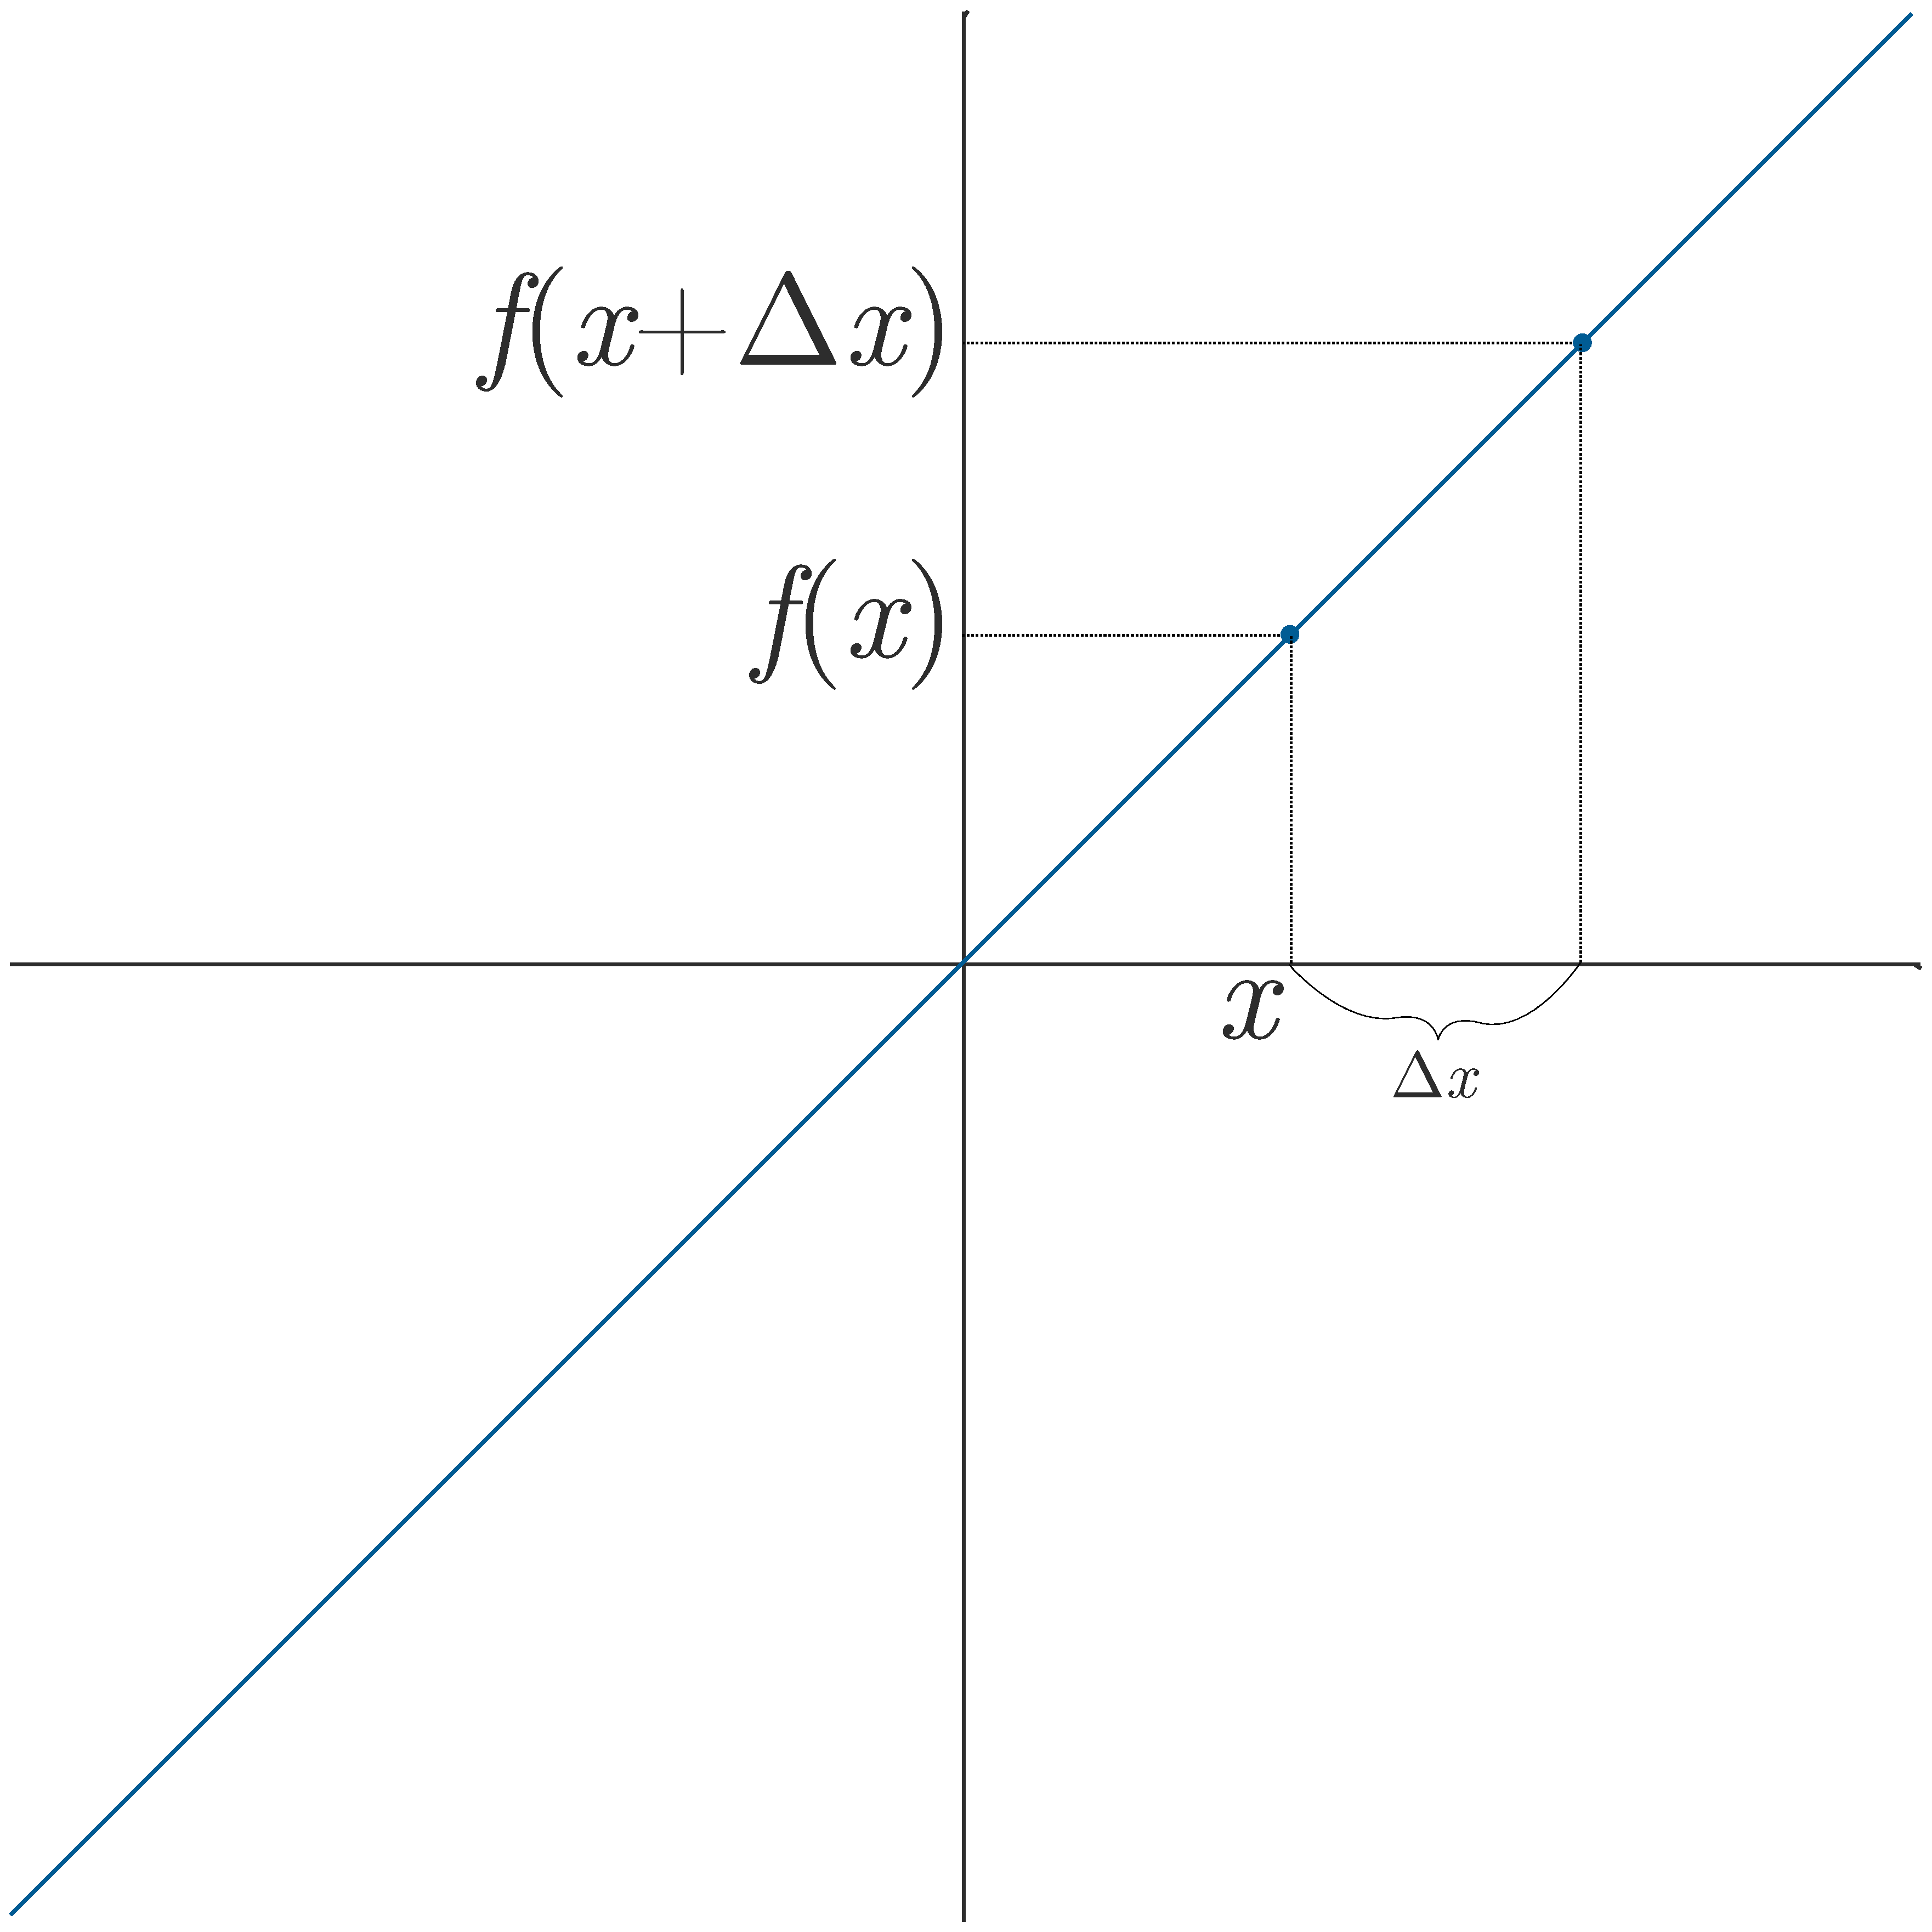
\includegraphics[width=0.5\textwidth]{continuous/derivatives/diffquot.eps}
  \end{center}
  \caption{A visual representation of the difference quotient on a line.}
\end{figure}
You'll often see the difference quotient written with $\Delta x \to h$ as
\begin{equation}
  \frac{\Delta f(x)}{\Delta x}=\frac{f(x+h)-f(x)}{h}
\end{equation}

\section{Derivatives}

\subsection{Limit Definition}

The difference quotient is used in the limit definition of the derivative, which is
\begin{equation}
  \label{eq:limitdef}
  \frac{\ud f(x)}{\ud x}=\lim_{h \to 0} \frac{f(x+h)-f(x)}{h}
\end{equation}
Notice that the only distinction between this equation and the difference quotient/slope equation from earlier is the introduction of a limit. The idea behind that limit is that you're calculating the slope of a function as the distance between your $x_2$ and $x_1$ values becomes infinitely small ($h\to 0$). We call this distance an \emph{infinitesimal}: a distance smaller than any feasible measurement, but not zero in size.

So what a derivative of a function is going to tell us is how the function behaves (its slope) at a particular ``infinitely small'' portion of the graph, which might as well be a point.

For linear functions, the function behaves the same no matter where you look at it, so their derivatives are always constant and equal to the slope of the function.

For nonlinear functions, like $f(x)=x^2$, the derivative will yield a function (in this case, just $f'(x)=2x$), because the function is changing its input values differently depending on where you are looking. Near the origin, where $x=0$, the derivative is zero and any $x$ value will give $y$ values not too far from the original input. But as you move further from the origin, the ratio of $y/x$ gets larger and larger, and the derivative in turn gets bigger and bigger.

\begin{figure}[H]
    \begin{center}
      
\includegraphics[width=0.5\textwidth]{continuous/derivatives/xsquared.eps}
      \caption{A graph of $f(x)=x^2$ and $f'(x)=2x$.}
    \end{center}
  \end{figure}

\subsection{Notation}

There are a number of ways to denote the derivative of a function $y=f(x)$. The most common notation early on in calculus classes is the \emph{prime} notation $y'$ and $f'$ because it is the simplest. Later on, you often see $\ud/\ud x$ style notation, because it is more specific. It tells us not only which function we are differentiating, but with respect to which variable. A notable characteristic of this ``d notation'' is the similarity it provides to our equation for slope:
\begin{align*}
  &m=\frac{\Delta y}{\Delta x}=\frac{\Delta f(x)}{\Delta x} &y'=\frac{\ud y}{\ud x}=\frac{\ud f(x)}{\ud x}
\end{align*}
In the case of slope, we're talking about specific $y$ and $x$ values, but in the case of a derivative, we're talking about \emph{infinitesimals}, and that particular distinction allows us to discuss the behavior of functions that aren't linear, but change their behavior over time.

\subsection{Tangent Lines}

The \emph{tangent line} to a graph at a point is just a line that acts like the function is linear and behaves exactly as the graph does at that point. This is useful for visualizing the derivative, and showing us how the behavior of a function can change depending on its $(x,y)$ location.

\begin{figure}[H]
  \begin{center}
    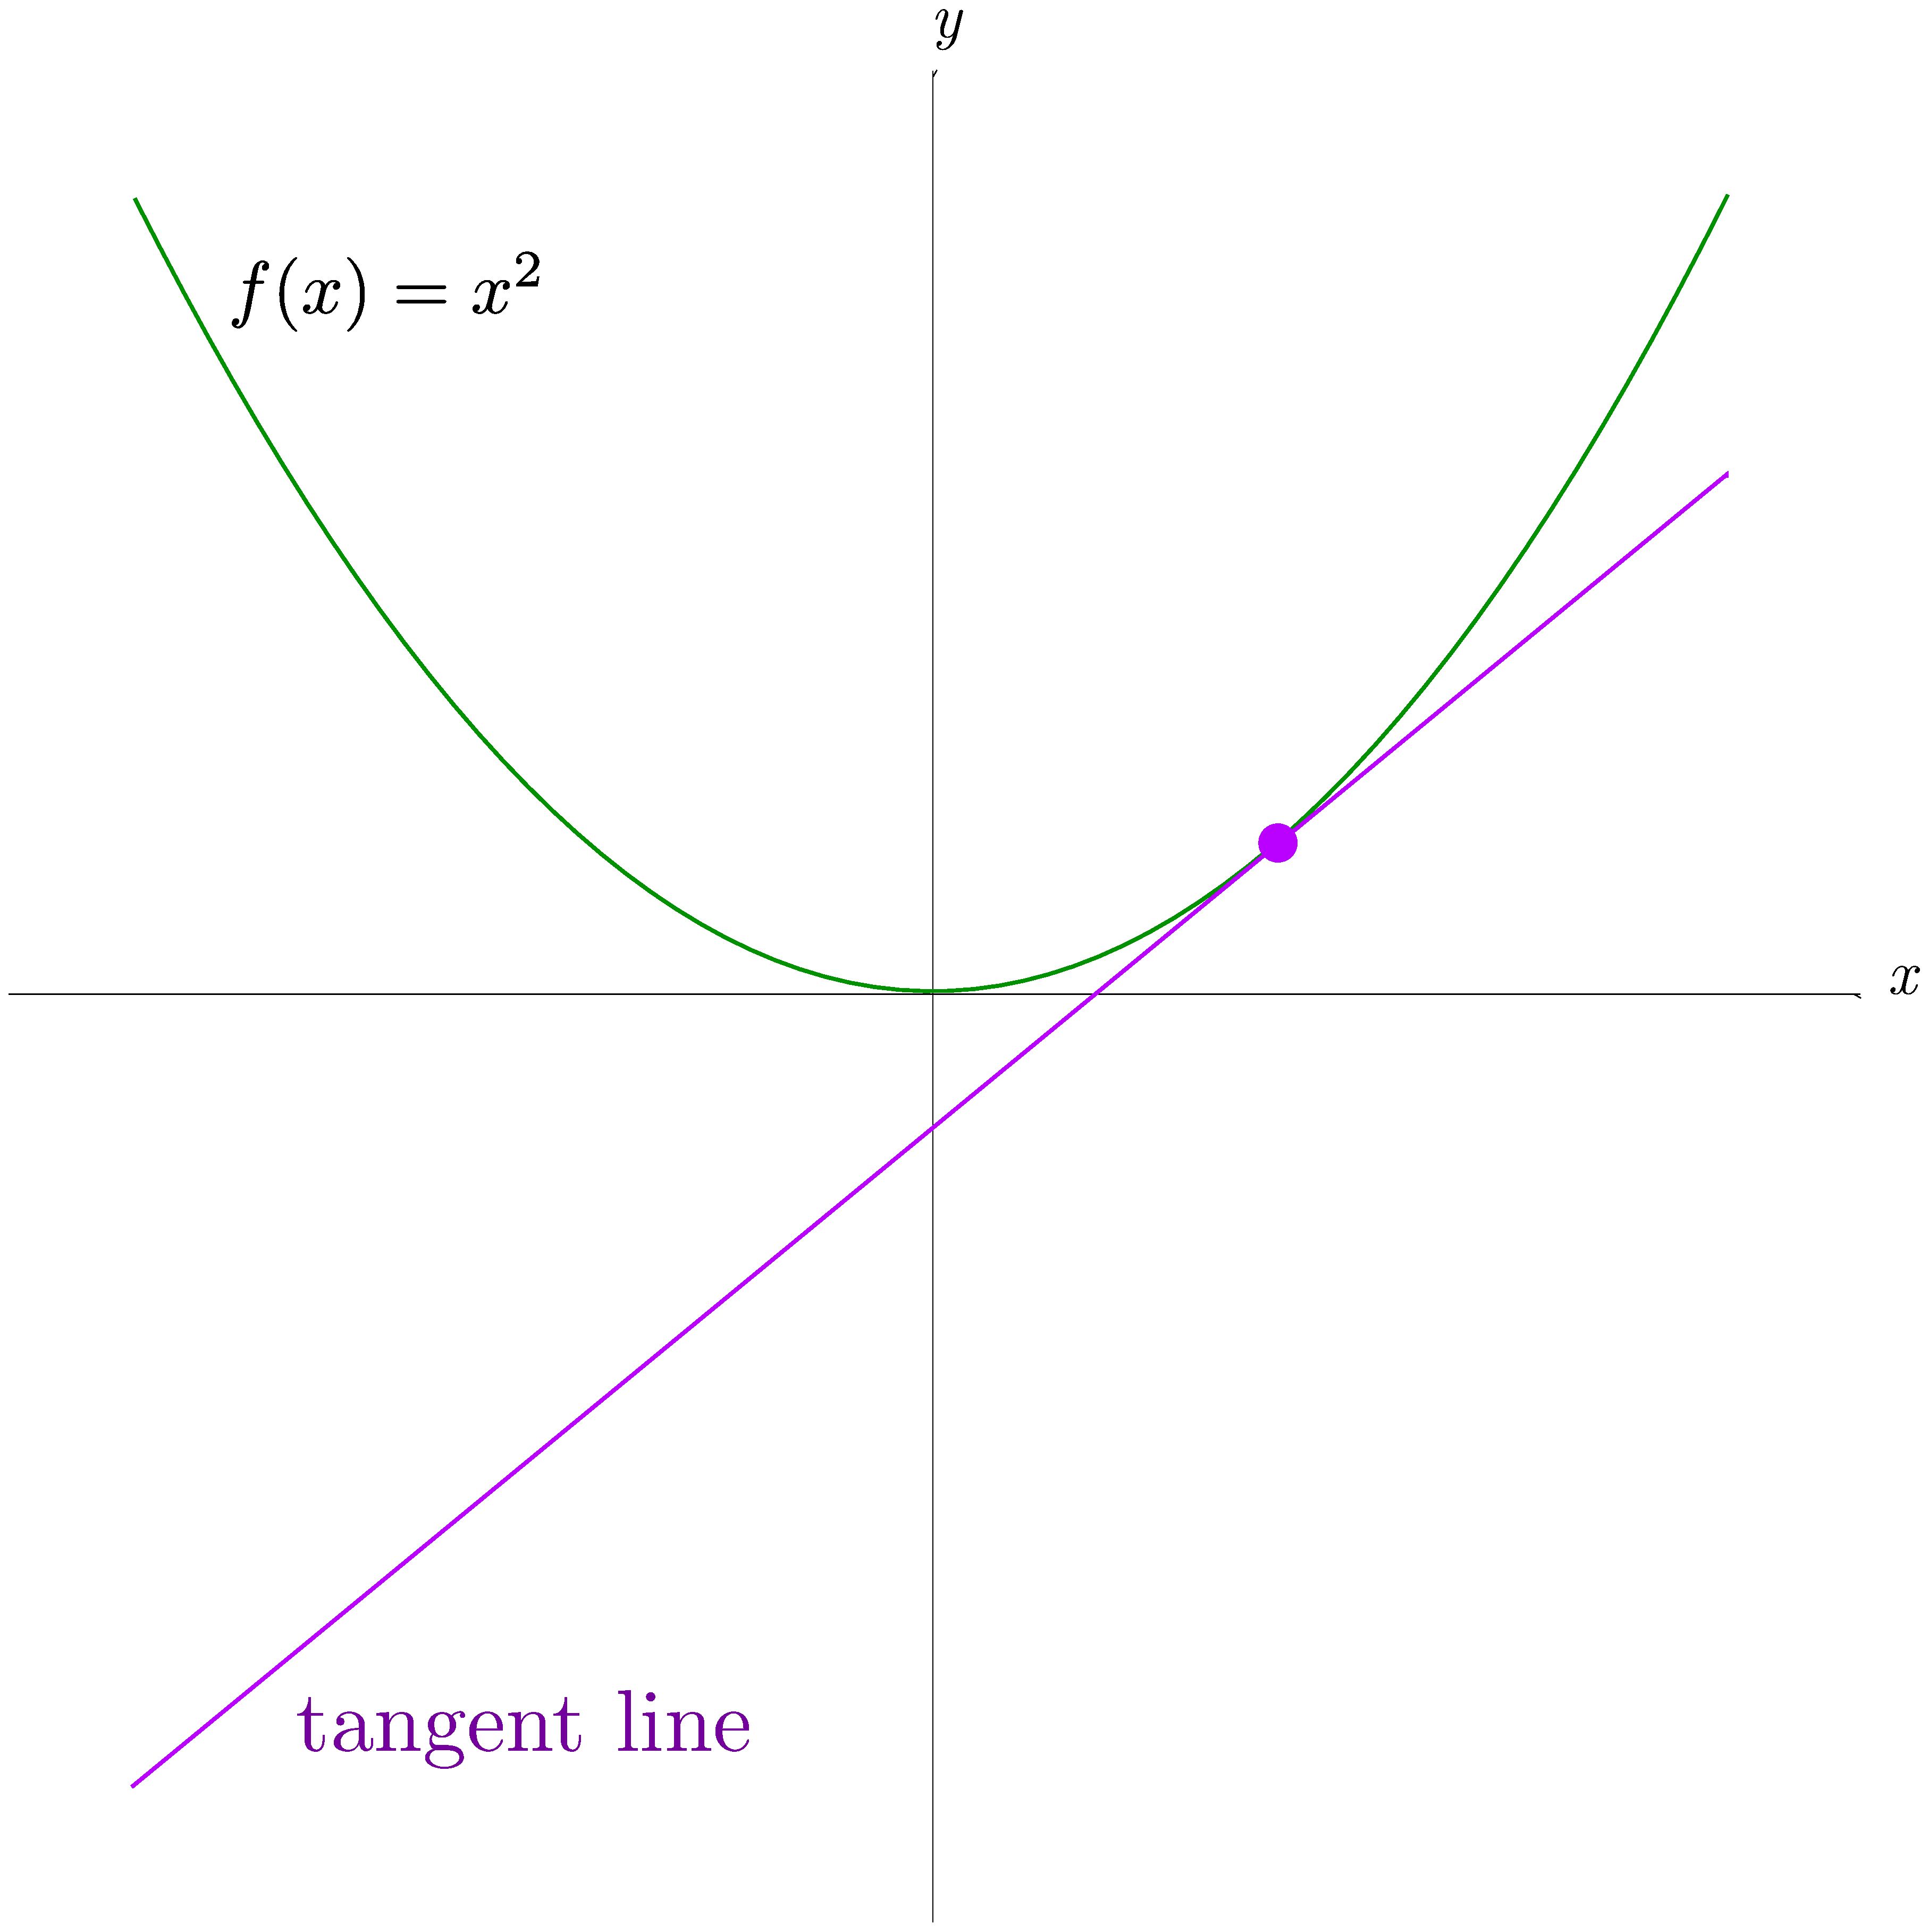
\includegraphics[width=0.4\textwidth]{continuous/derivatives/tangent.eps}
  \end{center}
  \caption{A tangent line to the graph of $f(x)=x^2$.}
\end{figure}

To calculate the equation for a tangent line at a point, simply find the
derivative of the function at that point and treat that as the slope of the
tangent line. Then, use the $(x, y)$ values of the point to produce the tangent line's function
using the point-slope equation (\eqref{eq:pointslope}).

\subsection{Derivative Rules}

Derivative rules are just shorthands for working things out manually using the
limit definition in equation \eqref{eq:limitdef}. They all come from equation \eqref{eq:limitdef}, but they serve as generalizations to greatly simplify the work we have to do in calculating derivatives.

\subsubsection{Power Rule}

The power rule states that
\begin{equation}
  \ddx x^n=nx^{n-1}
\end{equation}

\subsubsection{Product Rule}

The product rule states that
\begin{equation}
  \ddx (uv)=u \frac{\ud v}{\ud x}+v\frac{\ud u}{\ud x}
\end{equation}

\subsubsection{Quotient Rule}

The quotient rule states that
\begin{equation}
  \frac{\ud}{\ud x}\left(\frac{u}{v}\right)=\frac{v\frac{\ud u}{\ud x}-u\frac{\ud v}{\ud x}}{v^2}
\end{equation}

\subsubsection{Chain Rule}

The chain rule states that if $y=f(u)$ and $u=g(x)$, then
\begin{equation}
  \frac{\ud y}{\ud x}=\frac{\ud y}{\ud u} \cdot \frac{\ud u}{\ud x}
\end{equation}

The chain rule is used to differentiate composite functions, which look like $(f \circ g)(x)$ and mean $f(g(x))$. You'll want to develop an intuitive understanding for when to use the chain rule.
\begin{ex}
  Find the derivative of $f(x)$, where
  \[ f(x)=\frac{1}{x^3} \]
  \begin{figure}[h]
    \begin{center}
      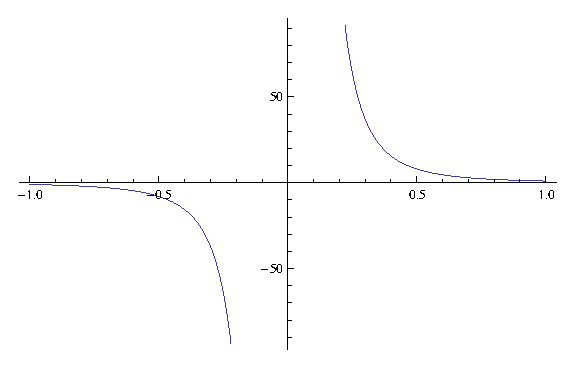
\includegraphics{continuous/derivatives/chainrule_1.eps}
    \end{center}
    \caption{A plot of $f(x)=\frac{1}{x^3}$.}
  \end{figure}
  \begin{sol}
    This is not a chain rule problem. Although you could think of it as one with $f(x)=1/x$ and $g(x)=x^3$, it is easier to remember that factors can be moved from the numerator to the denominator simply by multiplying their exponents by $-1$.
    \begin{align*}
      f(x)&=\frac{1}{x^3}\\&=x^{-3} \\
      \ddx f(x)&=-3x^{-4}
    \end{align*}
  \end{sol}
\end{ex}
\begin{ex}
  Find the derivative of $f(x)$, where
  $$ f(x)=\left(\frac{1}{\sqrt{x}}\right)^5 $$
  This is a chain rule problem. We use
  \begin{align*}
    & g(x)=\frac{1}{\sqrt{x}}
    & & f(x)={(g(x))^5}
  \end{align*}
  \begin{align*}
    \ddx f(x)&=\ddx \left(\frac{1}{\sqrt{x}}\right)^5 \\
      &= \ddx {(g(x))^5} \\
      &= 5g(x)^4 \cdot \ddx g(x)
  \end{align*}
  Now we find $ \ddx g(x) $
  \begin{align*}
    \ddx g(x) &= \ddx \frac{1}{\sqrt{x}} =\ddx \frac{1}{x^{1/2}} =\ddx x^{-1/2} \\
      &=\frac{-1}{2}x^{-3/2} =\frac{-1}{2x^{3/2}} \\
      &=\frac{-1}{2\sqrt{x^3}}
  \end{align*}
  and plug that back into our original derivative, along with $g(x)=\frac{1}{\sqrt{x}}$
  \begin{align*}
    \ddx f(x)&=5g(x)^4 \cdot \ddx g(x) \\
      &=5\left(\frac{1}{\sqrt{x}}\right)^4\cdot \frac{-1}{2\sqrt{x^3}}
  \end{align*}
  and simplify
  \begin{align*}
    \ddx f(x)&=5\left(\frac{1}{\sqrt{x}}\right)^4\cdot \frac{-1}{2\sqrt{x^3}} =5\left[\frac{1^4}{\left(\sqrt{x}\right)^4}\right] \cdot \frac{-1}{2\sqrt{x^3}} \\
    &=5\left[\frac{1}{\left(x^{1/2}\right)^4}\right] \cdot \frac{-1}{2\sqrt{x^3}}=5\left[\frac{1}{x^{4/2}}\right] \cdot \frac{-1}{2\sqrt{x^3}} \\
    &=5\left[\frac{1}{x^2}\right] \cdot \frac{-1}{2\sqrt{x^3}}=\frac{5}{x^2} \cdot \frac{-1}{2\sqrt{x^3}} \\
    &=\frac{-5}{2x^2\sqrt{x^3}} =\frac{-5}{2x^2\cdot x^{3/2}} \\
    &=\frac{-5}{2x^{4/2}\cdot x^{3/2}}\\
    &=\frac{-5}{2x^{7/2}} \\
  \end{align*}
\end{ex}
\subsection{Differentiability}
  A function $f(x)$ is differentiable at a point $x_0$ if a tangent line to its curve exists at that point and is not vertical. Functions are not differentiable at breaks, immediate bends, cusps, or places with vertical tangents.

\subsection{Graphing Functions}
To graph a function:
  \begin{enumerate}
   \item Find all \textbf{critical values}. Critical values are locations where $\frac{\ud y}{\ud x}=0$ or is undefined.\footnote{At locations where $\frac{\ud y}{\ud x}=0$, the tangent line is horizontal.}
   \item Find all \textbf{points of inflection}. These are locations where the second derivative ($\frac{\ud^2y}{\ud x}$) is zero or undefined.
   \item Determine where $\frac{\ud y}{\ud x}$ is \emph{positive} to find where $f(x)$ is \emph{increasing}. Remember that a derivative signifies the slope of a graph, so a positive derivative implies that the graph is increasing. This can be achieved either by testing values on each side of a \emph{critical value}, or by intuitive understanding. For example, $\frac{\ud y}{\ud x}=3x^2$ is positive everywhere except at $x=0$, so $f(x)=y$ is increasing everywhere except for at its horizontal tangent at $x=0$.\footnote{$x^2$ can never produce a negative number, because a negative times a negative or a positive times a positive is always positive}
   \item Determine where $\frac{\ud y}{\ud x}$ is \emph{negative} to find where $f(x)$ is \emph{decreasing}.
   \item Determine the sign of $\frac{\ud^2y}{\ud x}$ on both sides of all \emph{points of inflection}. The graph is \emph{concave up} where $\frac{\ud^2y}{\ud x}$ is positive, and \emph{concave down} where $\frac{\ud^2y}{\ud x}$ is negative.
  \end{enumerate}
\section{l'Hospital's Rule}\index{l'Hospital's Rule}

\textbf{l'Hospital's Rule} uses derivatives to calculate limits\index{limits} of fractions whose numerators and denominators both approach the same indeterminate for, which can be either zero or $\infty$. Limits involving transcendental functions\index{transcendental functions} often require some use of the rule for their calculation.

\begin{theorem}[L'Hospital's Rule]\label{th:lhospital}
  Suppose that $f(a)=g(a)=0$, that $f$ and $g$ are differentiable on an open interval $I$ containing $a$, and that $g'(x) \neq 0$ on $I$ if $x \neq a$. Then
  \[ \lim_{x \to a} \frac {f(x)}{g(x)} \=H \lim_{x \to a} \frac{f'(x)}{g'(x)} \]
  assuming that the limit on the right side of this equation exists.
\end{theorem}
\begin{remark}
  L'Hopital's Rule does not apply when either the numerator or the denominator has a finite nonzero limit.
\end{remark}
\begin{proof}
  We first establish the limit equation for the case $x \to a^+$. The method needs almost no change to apply to $x \to a^{-}$, and the combination of these two cases establishes the result.

  Suppose that $x$ lies to the right of $a$. Then $g'(x) \neq 0$, and we can apply Cauchy's Mean Value Theorem to the closed interval from $a$ to $x$. This step produces a number $c$ between $a$ and $x$ such that
  $$ \frac{f'(c)}{g'(c)}=\frac{f(x)-f(a)}{g(x)-g(a)} $$
  But $f(a)=g(a)$, so
  $$ \frac{f'(c)}{g'(c)}=\frac{f(x)}{g(x)} $$
  As $x$ approaches $a$, $c$ approaches $a$ because it always lies between $a$ and $x$. Therefore,
  $$ \lim_{x \to a^+} \frac{f(x)}{g(x)}=lim_{c \to a} \frac{f'(c)}{g'(c)} = lim_{x \to a^+} \frac{f'(x)}{g'(x)} $$
  which establishes l'Hospital's Rule for the case where $x$ approaches $a$ from
  above. The case where $x$ approaches $a$ from below is proved by applying
  Cauchy's Mean Value Theorem to the closed interval $[x,a], x <
  a$.\cite{thomas}
\end{proof}
\begin{figure}[h]
  \begin{center}
    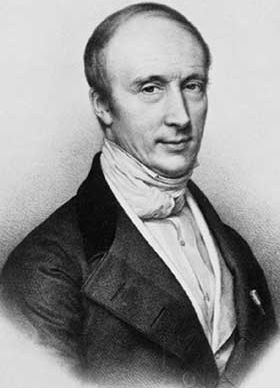
\includegraphics[width=0.2\textwidth]{photos/cauchy.jpg}
  \end{center}
  \caption{Augustin Louis Cauchy, 1901.}
\end{figure}
\begin{theorem}[Cauchy's Mean Value Theorem]\label{th:caunchymv}\index{Cauchy's Mean Value Theorem}
Suppose functions $f$ and $g$ are continuous on $[a, b]$ and differentiable throughout $(a, b)$ and also suppose $g'(x) \neq 0$ throughout $(a, b)$. Then there exists a number $c$ in $(a, b)$ at which
  \[ \frac {f'(c)}{g'(c)} = \frac{f(b)-f(a)}{g(b)-g(a)} \]
\end{theorem}
\section{Derivatives of Inverses of Differentiable Functions}\index{inverse
functions}

\begin{theorem}[The Derivative Rule for Inverses]\label{th:invderiv}
  If $f$ has an interval $I$ as domain and $f'(x)$ exists and is never zero on $I$, then $f^{-1}$ is differentiable at every point in its domain (the range of $f$). The value of $\big(f^{-1}\big)'$ at a point $b$ in the domain of $f^{-1}$ is the reciprocal of the value of $f'$ at the point $a=f^{-1}(b)$:
  \begin{equation}
    \big(f^{-1}\big)'(b)=\frac{1}{f'\big(f^{-1}(b)\big)} \qquad b \neq 0
  \end{equation}
  This can also be written
  \begin{equation}
    \cfrac{\ud f^{-1}}{\ud x}\bigg|_{x=b}=\cfrac{1}{\cfrac{\ud f}{\ud x}\bigg|_{x=f^{-1}(b)}}\qquad b \neq 0
  \end{equation}
  \begin{proof}
  Because a function applied to the inverse of itself should return its own input value, we can start with this relationship.
    \begin{align*}
      f \big( f^{-1}(x) \big) &= x \\
      \intertext{From here, take the derivative of both sides. On the left, we do so in notation only. On the right, we know that the derivative of a variable representing a constant is always 1.}
      \frac{\ud}{\ud x} f\big(f^{-1}(x)\big) &= 1\\
      \intertext{Because the lefthand side includes the composition of functions, we must use the chain rule in calculating its derivative. Applying the chain rule to the lefthand side of the equation gives us}
      f'\big(f^{-1}(x)\big)\cdot \cfrac{\ud}{\ud x}f^{-1}(x) &= 1  \\
      \intertext{Now, we divide each side of the equation by $f' \big( f^{-1}(x) \big)$ to solve for the derivative only, noting that $x$ cannot equal $0$.}
      \frac{\ud}{\ud x}f^{-1}(x) &= \cfrac{1}{f'\big(f^{-1}(x)\big)} \qquad x\neq 0
    \end{align*}
  \end{proof}
\end{theorem}

\chapter{Transcendental Functions}

A \textbf{transcendental function} is a function that does not satisfy a polynomial equation whose coefficients are themselves polynomials, in contrast to an algebraic function, which does satisfy such an equation.

In other words, a transcendental function is a function that ``transcends'' algebra in the sense that it cannot be expressed in terms of a finite sequence of the algebraic operations of addition, multiplication, and root extraction.

Examples of transcendental functions include the \emph{exponential function}, the \emph{logarithm}, and the \emph{trigonometric functions}.
%\cite{wiki:transcendental}

Formally,

\begin{defn}
  An analytic function \(f(z)\) of the real or complex variables \(z_1, \ldots, z_n\) is \textbf{transcendental} if the \(n+1\) functions \(z_1, \ldots, z_n\) are algebraically independent.
  \cite{wiki:transcendental}
\end{defn}

\section{Natural Logarithms}
\begin{figure}[h]
  \begin{center}
    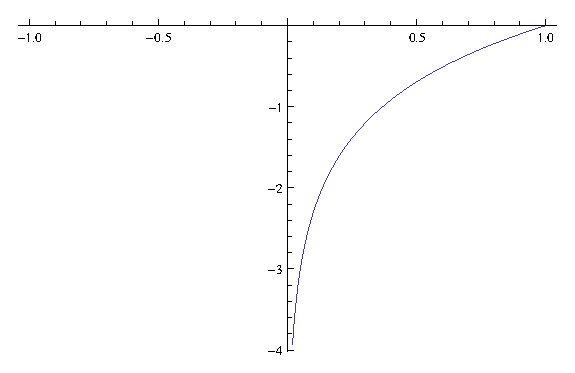
\includegraphics[width=0.4\textwidth]{continuous/transcend/natlog}
  \end{center}
  \caption{A plot of $f(x) =\ln x$.}
  \label{fig:natlog}
\end{figure}

\begin{defn}
  The \textbf{natural logarithm}\index{natural logarithm} is the function given by
  \begin{equation}
    \ln x = \int ^{x} _{1} \frac{1}{t} \ud t \text{,} \qquad x \in \mathbb{N}
  \end{equation}
\end{defn}
\begin{defn}
  The \textbf{number $e$} is that number in the domain of the natural logarithm satisfying
  \[ \ln{e}=1 \]
  It is roughly equal to
  \[2.7182818284590452353602874713526624977572470936999595\ldots\]
\end{defn}
\subsection{Algebraic Properties of the Natural Logarithm}

For any numbers $b>0$ and $x>0$, the natural logarithm satisfies the following rules:
\begin{table}[H]
    \begin{tabular}{p{3in}>\(p{3in}<\)}
      Product Rule      & \displaystyle{ \ln{bx}=\ln b + \ln x} \\\\
      Quotient Rule     & \displaystyle{ \ln{\frac{b}{x}}=\ln b - \ln x} \\ \\
      Reciprocal Rule   & \displaystyle{ \ln{\frac{1}{x}}=-\ln x} \\\\
      Power Rule        & \displaystyle{ \ln{x^r}=r \ln x \qquad \forall r \in \mathbb{R}}
    \end{tabular}
\end{table}
% \begin{equation}
% 	\ln{bx}=\ln b + \ln x
% \end{equation}
% \begin{equation}
% 	\ln{\frac{b}{x}}=\ln b - \ln x
% \end{equation}
% \begin{equation}
% 	\ln{\frac{1}{x}}=-\ln x
% \end{equation}
% \begin{equation}
% 	\forall r \in \mathbb{R} \quad \ln{x^r}=r \ln x
% \end{equation}

%The following table was sourced from \url{www.math.ualberta.ca/~apotapov/MATH115/ln-logs.pdf}:
\section{Logarithmic Identities}
\begin{align*}
  a^xa^y &=a^{x+y} & \log_a{(uv)}&=\log_a u+\log_a v \\
  (a^x)^y &= a^{xy} & \log_a{(u^y)} &= y\log_a u \\
  a^{-x} &= \frac{1}{a^x} & \log_a{\left(\frac{1}{u}\right)} &= -\log_a u \\
  \frac{a^x}{a^y} &= a^{x-y} & \log_a {\frac{u}{v}}&=\log_a u-\log_a v
\end{align*}

The number $e$ and its relationship to logarithms becomes especially important in integration,
where we manipulate its properties in calculus to solve equations and integrate functions we would not
otherwise be able to handle.

The inverse equations for $e^x$ and $\ln x$ are
\begin{equation}
  \forall (x>0)\big[e^{\ln x}=x\big]
  \label{eq:exinv1}
\end{equation}
\begin{equation}
  \forall x\big[\ln{(e^x)} =x\big]
  \label{eq:exinv2}
\end{equation}

The derivative of $e^x$ is very special, and it is
\begin{equation}
  \ddx e^x = e^x \ud x.
  \label{eq:ddxex}
\end{equation}


\section{Hyperbolic Functions}
Both \(\cos x\) and \(\sin x\) come from the formula for a circle.
\begin{equation}
  x^2 + y^2=r^2
  \label{eq:circle}
\end{equation}

But we can define other useful functions using the equation for a hyperbola.
\begin{equation}
  x^2-y^2=1
  \label{eq:hyperbola}
\end{equation}
Namely, \(\cosh x\) and \(\sinh x\).

In \ref{eq:hyperbola}, let \[ y \to \frac{e^x-e^{-x}}{2}\] to get \(\sinh x\).
Let \[ x \to \frac{e^x+e^{-x}}{2}\] to find \(\cosh x\).

We can prove that these still satisfy equation \ref{eq:hyperbola}:

\begin{proof}
  \begin{align*}
    1&=x^2-y^2 \\
    1&=\left( \frac{e^x+e^{-x}}{2} \right) - \left( \frac{e^x - e^{-x}}{2}
    \right)^2 \\
    1&=\frac{e^{2x}+2e^xe^{-x}+e^{-2x}}{4}-\frac{e^{2x}-2e^xe^{-x}+e^{-2x}}{4}
    \qedhere
  \end{align*}
\end{proof}

\chapter{Techniques of Integration}

\section{A Brief Table of Integrals}

\subsection{Basic Forms}

\begin{equation}
  \int k\,\ud x=kx+C \qquad \text{(any number \emph{k})}
\end{equation}
\begin{equation}
  \int x^n \, \ud x = \frac {x^{n+1}}{n+1}+C\,(n \neq -1)
\end{equation}
\begin{equation}
  \int \frac{\ud x}{x}=\ln{|x|}+C
\end{equation}
\begin{equation}
  \int e^x\, \ud x=e^x+C
\end{equation}
\begin{equation}
  \int a^x\, \ud x=\frac{a^x}{\ln a}+C \,(a>0,a\neq 1)
\end{equation}
\begin{equation}
  \int \sin x \, \ud x=-\cos x +C
\end{equation}
\begin{equation}
  \int \cos x \ud x=sin\,x+C
\end{equation}
\begin{equation}
  \int \sec^2x \ud x = \tan x + C
\end{equation}
\begin{equation}
  \int \csc^2 x \ud x = -cot\,x +C
\end{equation}
\begin{equation}
  \int \sec x \tan x \ud x = \sec x +C
\end{equation}
\begin{equation}
  \int \csc x \cot x \,dx = -\csc x +C
\end{equation}
\begin{equation}
  \int \cot x \ud x=\ln{|\sin x|}+C
\end{equation}
\begin{equation}
  \int \cosh x \ud x=\sinh x\,+C
\end{equation}
\begin{equation}
  \int \frac{\ud x}{a^2+x^2}=\frac{1}{a}\arctan{\frac{x}{a}}+C
\end{equation}
\begin{equation}
  \frac{\ud x}{\sqrt{a^2+x^2}}=\arcsin{\frac{x}{a}+C} \qquad (a > 0)
\end{equation}


\section{Integration by Parts}\index{integration by parts}
% rewrite this.
Integration by parts is used for simplifying integrals of the form
\[ \int f(x)g(x) \ud x \text{.} \]
It is useful when \(f\) can be differentiated repeatedly and $g$ can be integrated repeatedly without difficulty. The integrals
\[ \int x \cos x \ud x \quad \text{and} \quad \int x^2 e^x \ud x \]
are such integrals because $f(x)=x$ or $f(x)=x^2$ can be differentiated repeatedly to become zero, and $g(x)=\cos x$ or $g(x)=e^x$ can be integrated repeatedly without difficulty. Integration by parts also applies to integrals like
\[ \int \ln x \ud x \quad \text{and} \quad \int e^x \cos x \ud x \]
In the first case, $f(x)=\ln x$ is easy to differentiate and $g(x)=1$ easily integrates to $x$. In the second case, each part of the integrand appears again after repeated differentiation or integration.


\subsection{Integration By Parts Formula}

If $f$ and $g$ are differentiable functions of $x$, the Product Rule says that
$$ \frac{\ud}{\ud x} [f(x)g(x)]=f'(x)g(x)+f(x)g'(x) $$
In terms of indefinite integrals, this equation becomes
$$ \int \frac{\ud}{\ud x} [f(x)g(x)] \ud x=\int [f'(x)g(x)+f(x)g'(x)] \ud x $$
or
$$ \int \frac{\ud}{\ud x} [f(x)g(x)] \ud x=
\int f'(x)g(x) \ud x + \int f(x)g'(x) \ud x $$
Rearranging the terms of this last equation, we get
$$ \int f(x)g'(x) \ud x =
\int \frac{\ud}{\ud x}[f(x)g(x)]\ud x - \int f'(x)g(x) \ud x $$
Leading to the \textbf{integration by parts} formula
\begin{equation}
  \int f(x)g'(x)=f(x)g(x)-\int f'(x)g(x) \ud x
\end{equation}
Sometimes it is easier to remember the formula if we write it in differential form. Let $u=f(x)$ and $v=g(x)$. Then $\ud u=f'(x)\ud x$ and $\ud v=g'(x)\ud x$. Using the Substitution Rule, the \textbf{integration by parts} formula becomes
\begin{equation}
  \int u \ud v =  uv - \int v \ud u
  \label{equation:intbyparts}
\end{equation}

This formula expresses one integral, $\int u \ud v$, in terms of a second integral, $\int v \ud u$. With a proper choice of $u$ and $v$, the second integral may be easier to evaluate than the first.

\begin{ex}
  Integrate
  \[
    \int x \cos x \ud x.
    \]
    \begin{sol}
      We use integration by parts with
      \begin{align*}
        u&= x & \ud v &= \cos x \\
        \ud u &= \ud x & v &= \sin x
      \end{align*}
      So our integral becomes something we can integrate.
      \begin{align*}
        \int x \cos x \ud x &= x \sin x - \int \sin x \ud x \\
        &= x \sin x + \cos x +C
      \end{align*}
    \end{sol}
\end{ex}

% Rewrite this. Copied from textbook.
The goal of integration by parts is to go from an integral $\int u \ud v$ that we don't see how to evaluate to an integral $\int v \ud u$ that we can evaluate.
Generally, you choose $\ud v$ first to be as much of the integrand, including $\ud x$, as you can readily integrate; $u$ is the leftover part.
When finding $v$ from $\ud v$, any antiderivative will work and we usually pick the simplest one; no arbitrary constant of integration is needed in $v$ because it would simply cancel out on the right-hand side of \ref{equation:intbyparts}.

\begin{ex} A tough integration by parts problem.\footnote{Solved by Dr. James Martin, CNU Department of Mathematics. \url{http://math.cnu.edu/martin.htm}}
	\[ \int \frac{xe^{2x}}{(2x+1)^2}\ud x \]
  \begin{sol}
      We use integration by parts as follows:
      \begin{align*}
        u&=e^{2x} & \ud v&=\frac{x}{(2x+1)^2} \\
        \ud u &= 2e^{2x} & v &=\frac{1}{4+8x}+\frac{\ln{(1+2x)}}{4}
      \end{align*}
      To get:
      \begin{align*}
        \int \frac{xe^{2x}}{(2x+1)^2}\ud x
        =& \frac{e^{2x}}{4+8x}+\frac{e^{2x}\ln{|1+2x|}}{4}-\int 2e^{2x}\left[\frac{1}{4+8x}+\frac{\ln{(1+2x)}}{4}\right]\ud x \\
      \end{align*}
      Then we simplify the integrand.
      \begin{align*}
        \int \frac{xe^{2x}}{(2x+1)^2}\ud x =& \frac{e^{2x}}{4+8x}+\frac{e^{2x}\ln{|1+2x|}}{4}-\int \frac{2e^{2x}}{4+8x}\ud x-\frac{1}{2} \int e^{2x}\ln{|1+2x|}\ud x \\
        =& \frac{e^{2x}}{4+8x}+\frac{e^{2x}\ln{|1+2x|}}{4}-\frac{1}{2}\int \frac{e^{2x}}{1+2x}\ud x-\frac{1}{2} \int e^{2x}\ln{|1+2x|}\ud x
      \end{align*}
      We use integration by parts again on the second integral as follows:
      \begin{align*}
        u=&\ln{|1+2x|} & \ud v=&e^{2x} \\
        \ud u=&\frac{2}{1+2x}\ud x & v=& \frac{1}{2}e^{2x}
      \end{align*}
      \begin{align*}
        =& \frac{e^{2x}}{4+8x}+\frac{e^{2x}\ln{|1+2x|}}{4}
        -\frac{1}{2}\left[\frac{1}{2}e^{2x}\ln{|1+2x|}
          -\frac{1}{2} \int \frac{2e^{2x}}{1+2x} \ud x\right]
          -\frac{1}{2}\int \frac{e^{2x}}{1+2x}\ud x \\
          \intertext{We simplify our result, and all but one of the terms cancel:}
          =& \frac{e^{2x}}{4+8x}+\frac{e^{2x}\ln{|1+2x|}}{4}
          -\frac{1}{4}e^{2x}\ln{|1+2x|}
          + \frac{1}{2} \int \frac{e^{2x}}{1+2x} \ud x
          -\frac{1}{2}\int \frac{e^{2x}}{1+2x}\ud x \\
          =& \frac{e^{2x}}{4+8x}+\frac{e^{2x}\ln{|1+2x|}}{4}
          -\frac{e^{2x}\ln{|1+2x|}}{4}+C \\
          =& \frac{e^{2x}}{4+8x}+C
        \end{align*}
\end{sol}
\end{ex}
\begin{ex}
  Integrate
  \[\int\ln x \ud x.\]
  \begin{sol}
  Since $\int \ln x \ud x$ can be written as $\int \ln x \cdot 1 \ud x$, we can use integration by parts as follows:
  \begin{align*}
    u&=\ln x & \ud v &= \ud x \\
    \ud u &= \frac{\ud x }{x} & v&=x
  \end{align*}
  Which gives us the integral
  \begin{align*}
    \int\ln x \ud x &=
      x \ln x - \int  \frac{x \ud x}{x} \\
      &= x \ln x - \int \ud x \\
      &= x \ln x - x + C
    \end{align*}
  \end{sol}
\end{ex}

\subsection{Integration by Parts Cheat Sheet}
This is a set of guidlines\footnote{Proposed by Herbert Kasube of Bradley University.} advising whichever part of an integral comes first in this list should be assigned to $u$.
\begin{enumerate}
  \item Logarithms
  \item Inverse functions
  \item Algebraic
  \item Trigonometric
  \item Exponential
\end{enumerate}


\subsection{Reduction Formulas}
% probably rewrite this. I think I might have too much unoriginal material in this section.
Consider the integral
\begin{align*}
  I_n=&\int x^n e^{ax} \ud x
  \intertext{Integration by parts gives you}
  I_n=&x^n \frac{1}{a}e^{ax}-\int nx^{n-1}\frac{1}{a}e^{ax}\ud x \\
     =&\frac{1}{a}x^ne^{ax}-\frac{n}{a}\int x^{n-1}e^{ax}\ud x
\end{align*}
We haven't computed the integral. What we have done is derived the following \textbf{reduction formula}
\begin{equation}
  I_n=\frac{1}{a}x^ne^{ax}-\frac{n}{a}I_{n-1}
\end{equation}
which holds for all $n$.

For $n=0$ the reduction formula says
$$ I_0=\frac{1}{a}e^{ax} \to \int e^{ax}\ud x = \frac{1}{a}e^{ax}+C $$

When $n \neq 0$ the reduction formula tells us that we have to compute $I_{n-1}$ if we want to find $I_n$. The point of a reduction formula is that the same formula also applies to $I_{n-1}$, and $I_{n-1}$, etc. so that after repeated application of the formula we end up with $I_0$, an integral we know how to compute.\cite{freenotes}
\begin{ex}
  %[textbook: \#4/pg.441]
  Integrate
  \[ \int e^x \cos x \ud x \]
  \begin{sol}
    We use integration by parts with
    \begin{align*}
      u &= \cos x & \ud v &= e^x \ud x \\
      \ud u &= - \sin x \ud x & v &=e^x
    \end{align*}
    Which gives us the integral
    \begin{align*}
      \int e ^x \cos x \ud x &= e^x \cos x - \int -e^x \sin x \ud x \\
      &= e^x \cos x+ \int e^x \sin x \ud x \\
      \intertext{Now we use $u$-substitution with $u=e^x$ and $\ud u = e^x \ud x$.}
      &= e^x \cos x + \int \sin u \ud u \\
      &= e^x \cos x - \cos u +C \\
      &= e^x \cos x - \cos {e^x} +C
    \end{align*}
  \end{sol}
\end{ex}
\begin{ex}
  Integrate
  \[ \int (1-x)^{9}\ud x. \]
  \begin{sol}
    This is not an integration by parts problem.
    It is just a regular $u$-substitution and power rule problem.
    Let $u=1-x$ and $\ud u = -\ud x$.
    \begin{align*}
      \int (1-x)^9 \ud x &= -\int u ^9 \\
      &= -\frac{u^{10}}{10}+C\\
      &= -\frac{(1-x)^{10}}{10}+C
    \end{align*}
  \end{sol}
\end{ex}
\begin{ex}
  Integrate:
  \[
    \int 3x^2 \cos x^3 \ud x
    \]
  \begin{sol}
    Again, this is not an integration by parts problem.
    Because we can spot the derivative of $x^3$ clearly in the integrand,
    we can let $u=x^3$ and $\ud u = 3x^2 \ud x$.
    \begin{align*}
      \int 3x^2 \cos x^3 \ud x & = \int \cos u \ud u \\
      &= \sin u +C\\
      &= \sin {x^3}+C
    \end{align*}
  \end{sol}
\end{ex}
\begin{ex}
  Integrate
  \[
    \int x \cos x \ud x
    \]
    \begin{sol}
      Use integration by parts with
      \begin{align*}
        u &= x & \ud v &= \cos x \ud x \\
        \ud u &= \ud x & v &= \sin x
      \end{align*}
      Which gives us
      \begin{align*}
        \int x \cos x \ud x &= x \sin x - \int \sin x \ud x \\
        &= x \sin x + \cos x +C
      \end{align*}
    \end{sol}
\end{ex}
\begin{ex}
  Integrate
  \[
    \int x e^x \ud x
    \]
    \begin{sol}
      Use integration by parts with
      \begin{align*}
        u&=x & \ud v &= e^x \ud x \\
        \ud u &= \ud x & v &= e^x
      \end{align*}
      \begin{align*}
        \int x e^x \ud x &= x e^x -\int e^x \ud x \\
        &=x e^x -e^x +C
      \end{align*}
    \end{sol}
\end{ex}
\begin{ex}
  Integrate
  \[
    \int x \ln x \ud x
    \]
  \begin{sol}
    Use integration by parts with
    \begin{align*}
      u&= \ln x & \ud v &= x \ud x \\
      \ud u &= \frac{\ud x}{x} & v &= \frac{x^2}{2}
    \end{align*}
    Which gives us
    \begin{align*}
      \int x \ln x &= \frac{x^2 \ln x}{2}- \int \frac{x^2 \ud x}{2x} \\
      &= \frac{x^2 \ln x}{2}-\frac{1}{2} \int x \ud x \\
      &= \frac{x^2 \ln x}{2}-\frac{x^2}{4}+C
    \end{align*}
  \end{sol}
\end{ex}
\begin{ex}
  \[
    \int x e^{x^2} \ud x
    \]
    \begin{sol}
      This looks like an integration by parts problem at first, but again it is just a regular $u$-substitution problem.
      Let $u=x^2$ and $\ud u=2x\ud x$.
      \begin{align*}
        \int x e^{x^2} \ud x &= \frac{1}{2}e^u \ud u \\
        &= \frac{1}{2} e^u +C \\
        &= \frac{1}{2}e^{x^2} +C
      \end{align*}
    \end{sol}
\end{ex}
% PLEASE rewrite this section ASAP.
% Clean it up, add descriptions, put it in proper format, etc.
% This is priority #1 for now.
%
%  \begin{ex}
%    \[ \int x^3 e^{x^2} \ud x \]
%    Don't be discouraged if your first attempt at integration by parts fails.
%    \begin{align*}
%      u &= x^{3} & dv &= e^{x^{2}} \\
%      \ud u &= 3x^{2} \ud x & v &= \text{?}
%    \end{align*}
%    Just try again:
%    \begin{align*}
%      u &= x^2 & dv &= x e^{x^2} \ud x \\
%      \ud u &= 2x \ud x & v &= \frac{e^{x^2}}{2}
%    \end{align*}
%    \begin{align*}
%      \int x^3 e^{x^2} \ud x &=
%      \frac{x^2 e^{x^2}}{2} - \int \frac{2}{2} x e^{x^2} \ud x
%      =\frac {x^2 e^x}{2}- \frac {e^{x^2}}{2} + C \\
%      &=\frac{x^2 e^x-e^x}{2}+C
%    \end{align*}
%  \end{ex}
%  \begin{ex}
%    \[ \int e^x (x+1)^2 \ud x \]
%    Start with integration by parts:
%    \begin{align*}
%      u &= (x+1)^2 & \ud v &= e^x \ud x \\
%      \ud u &= 2(x+1)\ud x & v &= e^x
%    \end{align*}
%    \begin{align*}
%      \int e^x (x+1)^2 \ud x&=
%        e^x (x+1)^2 - \int e^x 2(x+1)\ud x \\
%      &=e^x (x+1)^2 - 2\int e^x (x+1)\ud x
%    \end{align*}
%    Saving this for later...
%    \begin{comment}
%    Then use integration by parts again:
%    \begin{align*}
%      u &= x+1 & \ud v &= e^x \ud x \\
%      \ud u &= \ud x & v &= e^x
%    \end{align*}
%    \begin{align*}
%      \int e^x (x+1)^2 \ud x&=
%        e^x (x+1)^2 - 2\left[e^x(x+1)-\int e^x \ud x \right] \\
%      &=e^x (x+1)^2 - 2[e^x(x+1)-e^x] + C \\
%      &=e^x (x+1)^2 - 2e^x(x+1)+2e^x + C\\
%      &=x^2e^x+e^x-2xe^x-2e^x+2e^x+C
%    \end{align*}
%    \end{comment}
%  \end{ex}
%  \begin{ex}
%    Another ``strange'' integral:
%    \[ \int \arcsin x \ud x \]
%  \end{ex}
%  \begin{ex}
%    \[ \int \sin^{-1}x \ud x \]
%    \begin{align*}
%      u &= \sin^{-1}x & \ud v&=\ud x\\
%      \ud u &= \frac {1}{\sqrt{1-x^2}} \ud x & v &= x
%    \end{align*}
%    \begin{align*}
%      \int \sin^{-1}x \ud x &=
%      x \sin^{-1}x - \underbrace{\int \frac {x}{\sqrt{1-x^{2}}} \ud x}_{\lets u = 1-x^{2}}=x \sin^{-1}x-\frac{1}{2} \int \frac{\ud u}{\sqrt{u}} \\
%      &=x \sin^{-1}x+\frac{1}{2} \int u^{-1/2}\ud u=x sin^{-1}x+\sqrt u +C \\
%      &=x \sin^{-1}x+\sqrt{1-x^{2}} +C
%    \end{align*}
%  \end{ex}
%  \begin{ex}
%    \[ \int 4x e^{4x} \ud x \]
%    \begin{sol}
%    We use integration by parts with
%    \begin{align*}
%      u&=x & \ud v&=e^{4x}\ud x \\
%      \ud u &=\ud x & v &=\frac{1}{4}e^{4x}
%  	\end{align*}
%  	\begin{align*}
%  	  \frac{1}{x^4+2x^2+1}
%  	    =&4\left[x \cdot \frac{1}{4}e^{4x}-\int 1 \cdot \frac{1}{4} e^{4x} \ud x\right] \\
%  	    =&4\left[x \cdot \frac{1}{4}e^{4x}-\frac{1}{4}\int e^{4x} \ud x\right] \\
%  	    =& x e^{4x}-\frac{1}{4}e^{4x} + C
%    \end{align*}
%  \end{sol}
%  \end{ex}
%
%  % \begin{homework}
%  % pg. 489 odd 1-7, pg. 441 odd 1-23, pg. 441 6, 8, 35, 39.
%  % \end{homework}
%
%  \begin{ex}[\#23/pg.441]
%    \[ \int e^{2x}\cos{3x}\ud x \]
%    \begin{align*}
%      u &= \cos{3x} & \ud v&=e^{2x}\ud x\\
%      \ud u &= -3\sin{3x}\ud x & v&=\frac{1}{2}e^{2x}
%    \end{align*}
%    \begin{align*}
%      \int e^{2x}\cos{3x}\ud x &=
%        \frac{1}{2}e^{2x}\cos{3x}+\frac{3}{2}\int e^{2x}\sin{3x}\ud x \\
%      &=\frac{1}{2}e^{2x}\cos{3x}+\frac{3}{2}
%        \left[\frac{1}{2}e^{2x}\sin{3x}-\frac{3}{2}\int e^{2x}\cos{3x}\ud x \right]\ \\
%      \to\frac{4}{4}\int e^{2x}\cos{3x}\ud x
%        &=\frac{1}{2}e^{2x}\cos{3x}+\frac{3}{4}e^{2x}\sin{3x}-\frac{9}{4}\int e^{2x}\cos{3x}\ud x \\
%      \frac{13}{4}\int e^{2x}\cos{3x}\ud x
%        &=\frac{1}{2}e^{2x}\cos{3x}+\frac{3}{4}e^{2x}\sin{3x}+C \\
%      13\int e^{2x}\cos{3x}\ud x
%        &=2e^{2x}\cos{3x}+3e^{2x}\sin{3x}+C \\
%      \int e^{2x}\cos{3x}\ud x
%        &=\frac{2}{13}e^{2x}\cos{3x}+\frac{3}{13}e^{2x}\sin{3x}+C \\
%      &=\frac{e^{2x}}{13}\left[2\cos{3x}+3\sin{3x}\right]+C
%    \end{align*}
%    % Old in-class garbage:
%    % $$\frac{1}{2}cos(3x)e^{2x}+\frac{3}{2}\int e^{2x}sin(3x)\ud x \frac{1}{2}cos(3x)e^{2x}+\frac{3/2} (\frac{1}{2}e^{2x}sin(3x)-\frac{3}{2}\int e^{2x}cos(3x)\ud x)
%  \end{ex}
%  \begin{ex}
%    Integrate
%    \[ \int x^2\cos{3x}\ud x \]
%    \begin{sol}
%      Use integration by parts.
%      \begin{align*}
%        u&=x^2 && \ud v=\cos{3x}\ud x \\
%        \ud u=&2x\ud x && v=\frac{1}{3}\sin{3x}
%      \end{align*}
%      \begin{align*}
%        \int x^2\cos{3x}\ud x
%        =nt^{a}_{-\infty} f(x) \ud x
%            + \int^{\infty}_{a} f(x) \ud x& \frac{1}{3}x^2\sin{3x}-\frac{2}{3}\int x \sin{3x} \ud x \\
%        \intertext{Now use integration by parts again}
%        =& \frac{1}{3}x^2\sin{3x}-\frac{2}{3} \left( \frac{-x}{3}\cos{3x}+\frac{1}{3}\int\cos{3x}\ud x \right)\\
%        =& \frac{1}{3}x^2\sin{3x}+\frac{2}{9}x\cos{3x}-\frac{2}{27}\sin{3x}+C
%      \end{align*}
%    \end{sol}
%  \end{ex}
%  \begin{ex}
%    Integrate
%    \[ \int \frac{x}{\sqrt{x+3}} \]
%    \begin{sol}
%    Use integration by parts with
%    \begin{align*}
%      u&=x  & \ud v&=\frac{\ud x}{\sqrt{x+3}} \\
%      \ud u&=\ud x & v &=2\sqrt{x+3}
%    \end{align*}
%    \begin{align*}
%      \int \frac{x}{\sqrt{x+3}} =& 2x\sqrt{x+3}-\int 2\sqrt{x+3}\ud x \\
%      =& 2x \sqrt{x+3}-\frac{4}{3}(x+3)^{3/2}+C
%    \end{align*}
%  \end{sol}
%  \end{ex}
%  \begin{ex}
%    Integrate
%    \[\sin^{-1}{3x}\ud x\]
%    \begin{sol}
%      We use integration by parts with
%      \begin{align*}
%        u&=\arcsin{3x} & \ud v &= \ud x \\
%        \ud u &=\frac{3}{\sqrt{1-9x^2}}\ud x & v&=x
%      \end{align*}
%      \begin{align*}
%        \arcsin{3x}\ud x
%        =&x\arcsin{3x}-\int \frac{3x \ud x}{\sqrt{1-9x^2}} \\
%        =&x\arcsin{3x}+\frac{1}{3}\sqrt{1-9x^2}+C
%      \end{align*}
%    \end{sol}
%  \end{ex}


\section{Trigonometric Integrals}

Trigonometric integrals involve algebraic combinations of the six basic trigonometric functions. In principle, we can always express such integrals in terms of sines and cosines, but it is often simpler to work with other functions, as in the integral
$$ \int sec^2 x \ud x = \tan x + C $$
The general idea is to use identities to transform the integrals we have to find into integrals that are easier to work with.

We begin with integrals of the form:
$$ \int \sin^mx\cos^nx\ud x $$
where $m$ and $n$ are nonnegative integers (positive or zero). We can divide the appropriate substitution into three cases according to $m$ and $n$ being odd or even.
\begin{enumerate}
  \item If \textbf{$m$ is odd}, we write $m$ as $2k+1$ and use the identity $\sin^2x=1-\cos^2x$ to obtain
  $$sin^mx=sin^{2k+1}x=(sin^2x)^k\sin x=(1-\cos^2x)^k\sin x $$
  Then we combine the single $\sin x$ with $\ud x$ in the integral and set $\sin x \ud x$ equal to $-\ud (\cos x)$.
  \item If \textbf{$m$ is even and $n$ is odd} in $\int \sin^mx\cos^nx \ud x$, we write $n$ as $2k+1$ and use the identity $\cos^2x=1-\sin^2x$ to obtain
  $$ \cos^nx=\cos^{2k+1}x=(\cos^2x)^k\cos x=(1-\sin^2x)^k\cos x $$
  We then combine the single $\cos x$ with $\ud x$ and set $\cos x \ud x$ equal to $d(\sin x)$.
  \item If \textbf{both $m$ and $n$ are even} in $\int \sin^mx\cos^nx\ud x$, we subsitute
  \begin{align*}
    &\sin^2x=\frac{1-\cos{2x}}{2}
    &\cos^2x=\frac{1+\cos{2x}}{2}
  \end{align*}
  to reduce the integrand to one in lower powers of $\cos{2x}$.
\end{enumerate}

We can also use trigonometric identities to eliminate square roots in integrals:
\begin{ex}
  \[ \int^{\frac{\pi}{4}}_{0} \sqrt{1+\cos{4x}}\ud x \]
  To eliminate the square root, we use the identity
  \[ \cos^2 \theta = \frac{1+\cos{2 \theta}}{2} \]
  With $\theta=2x$, this becomes:
  \[ 1+\cos{4x}=2\cos^2{2x} \]
  Therefore,
  \begin{align*}
    \int^{\frac{\pi}{4}}_{0} \sqrt{1+\cos{4x}}\ud x&= \int^{\frac{\pi}{4}}_{0} \sqrt{2 \cos^2{2x}} \ud x = \int^{\frac{\pi}{4}}_{0} \sqrt2 \sqrt{\cos^2{2x}} \\
    &= \sqrt2 \int^{\frac{\pi}{4}}_{0} |\cos{2x}|\ud x = \sqrt2 \int^{\frac{\pi}{4}}_{0} \cos{2x}\ud x \\
    &= \sqrt2 \left[\frac{\sin{2x}}{2}\right]^{\frac{\pi}{4}}_{0} = \frac{\sqrt2}{2}[1-0] \\
    &= \frac{\sqrt2}{2}
  \end{align*}
\end{ex}


\subsection{Examples}
\begin{comment}
  I don't like how this is structured.
  \begin{itemize}
      \item $ \int tan^{\text{power}}x \, sec^{\text{even}}x\ud x$
      \item $ \int \underbrace{sin^{\text{power}x} \, cos^{\text{power}}x \ud x}_{\text{except where both are even}} $
      \item $ \int cot^{\text{power}x} \, csc^{\text{even}}x \ud x $
      \item $ \int sin(mx) \,  sin(nx) \ud x = \int \frac{1}{2}(cos(m-n)x-cos(m+n)x)$
      \item $ \int cos(mx) \,  cos(nx) \ud x = \int \frac{1}{2}(cos(m-n)x-cos(m+n)x)$
  \end{itemize}
\end{comment}

\begin{ex}
  \[ \int \sin^7x \cos^2x \ud x \]
  \begin{sol}
  \begin{align*}
    \int \sin^7x \cos^2x \ud x &=
      \int \sin^6x \cos^2x \sin x \ud x \\
    &=(\sin^2x)^3\cos^2x\sin x\ud x \\
    \intertext{because $\sin^2x=1-\cos^2x$}
    &=(1-\cos^2x)^3 \cos^2x\sin x \ud x
    \intertext{let $u=\cos x$ and $\ud u=-\sin x$.}
    &=-\int(1-u^2)^3u^2\ud u \\
    &=-\int (1-u^2)(1-u^2)(1-u^2)u^2\ud u \\
    &=-\int(1-2u^2+u^4)(1-u^2)u^2 \ud u \\
    &=-\int(u^2-2u^4+u^6-u^4+2u^6-u^8)\ud u \\
    &=\frac{-u^3}{3}+\frac{2u^5}{5}-\frac{u^7}{7}+\frac{u^5}{5}-\frac{2u^7}{7}+\frac{u^9}{9}+C \\
    &=\frac{-\cos^3x}{3}+\frac{2\cos^5x}{5}-\frac{\cos^7x}{7}+\frac{\cos^5x}{5}-\frac{2\cos^7x}{7}+\frac{\cos^9x}{9}+C
  \end{align*}
\end{sol}
\end{ex}
\begin{ex}
	\[ \int \cos^7x \sin^2x \ud x \]
	\begin{sol}
	\begin{align*}
		\int \cos^7x \sin^2x \ud x &=
		  \int \cos^6x \sin^2x \cos x \ud x
		\intertext{Because $\cos^2x=1-\sin^2x$:}
		&=\int (1-\sin^2x)^3\sin^2x\cos x \ud x \\
		\intertext{Now let $u=\sin x$ and $\ud u=\cos x \ud x$.}
		&= \int(1-u^2)^3u^2 \ud u \\
		&= \int (u^2-2u^4+u^6-u^4+2u^6-u^8) \ud u \\
		&= \frac{u^3}{3}-\frac{2u^5}{5}+\frac{u^7}{7}-\frac{u^5}{5}+\frac{2u^7}{7}-\frac{u^9}{9}+C \\
		&= \frac{\sin^3x}{3}-\frac{2\sin^5x}{5}+\frac{\sin^7x}{7}-\frac{\sin^5x}{5}+\frac{2\sin^7x}{7}-\frac{\sin^9x}{9}+C \\
		&= \frac{\sin^3x}{3}-\frac{\sin^5x}{5}+\frac{3\sin^7x}{7}-\frac{\sin^9x}{9}+C
	\end{align*}
\end{sol}
\end{ex}
\begin{ex}
	\[\int \sin^{15}x\ud x \]
	\begin{sol}
	\begin{align*}
		\int \sin^{15}x\ud x&=\int sin^{14}x \sin x \ud x =\int (\sin^2x)^7 \sin x \ud x \\
	  &=\int (1-\cos^2x)^7 \sin x \ud x
	  \intertext{Let $u=\cos x$ and $\ud u=-\sin x \ud x$.}
	  &=-\int (1-u^2)^7 \ud u =-\int \ud u + \int u^{14} \ud u=-u+\frac{u^{15}}{15}+C \\
	-  &=-\cos x + \frac{\cos^{15}x}{15}+C
	\end{align*}
\end{sol}
\end{ex}
\begin{ex}
  \[ \int \sin^2x \cos^2x \ud x \]
  \begin{sol}
    Remembering our power reduction identities from \eqref{eq:cossqq} and \eqref{eq:sinsqq}:
  \begin{align*}
	  \int \sin^2x \cos^2x \ud x &=\int \frac{1-\cos{2x}}{2} \cdot \frac{1+\cos{2x}}{2} \ud x =\frac{1}{4} \int (1-\cos^2{2x})\ud x \\
	  &= \frac{1}{4} \int \left(\frac{2}{2}-\frac{1+\cos{4x}}{2}\right)\ud x
	  =\frac{1}{4} \int \left(\frac{2-(1+\cos{4x})}{2}\right)\ud x \\
	  &=\frac{1}{4} \int \left(\frac{1-\cos{4x})}{2}\right)\ud x
	  =\frac{1}{8}\int 1-\cos{4x}\ud x \\
	  &=\frac{1}{8}\int \ud x - \frac{1}{8} \int \cos{4x}\ud x \\
	  &=\frac{x}{8}-\frac{1}{32}\sin{4x}+C
	\end{align*}
\end{sol}
\end{ex}
\begin{ex}
	\[ \int \tan^6x \sec^4x \ud x\]
	\begin{sol}
	\begin{align*}
		\int \tan^6x \sec^4x \ud x&=\int \tan^6x \sec^2x \sec^2x \ud x
		\intertext{Remembering that $\sec^2x=1+\tan^2x$:}
		&=\int \tan^6x (1+\tan^2x) \sec^2x \ud x
		\intertext{Now, letting $u=\tan x$ and $\ud u=\sec^2x\ud x$:}
		&= \int u^6(1+u^2)\ud u
		= \int u^6\ud u + \int u^8\ud u
		=\frac{u^7}{7}+\frac{u9}{9}+C \\
		&=\frac{\tan^7x}{7}+\frac{\tan^9x}{9}+C
	\end{align*}
\end{sol}
\end{ex}
\begin{ex}
  $$ \int cot^{8}x \, csc^{4}x \ud x $$
\end{ex}

% \begin{homework}
% Read section 8.2 and solve pg. 448 1-12,13,15,33,37,38,45,47,50,51,53,55,63,65,67
% \end{homework}


\section{Trigonometric Substitution}

\textbf{Trigonometric substitution} is the substitution of trigonometric functions for other expressions. One may use the trigonometric identities to simplify certain integrals containing radical expressions.

There are two important trig identities for us to know in this section:
\[ 1-sin^{2}\theta=cos^{2}\theta \]
\[ 1+tan^{2}\theta=sec^{2}\theta \]

We will find trigonometric substitution useful for problems that look this:

\[ \int \frac{dx} {x \sqrt{x^{2}-4}} \]

For integrands with $ \sqrt{x^{2}-a^{2}}$, $\lets x=a\sec \theta$ and let $\ud x = a \sec \theta \tan \theta \ud \theta $.
\begin{figure}[H]
  \begin{center}
    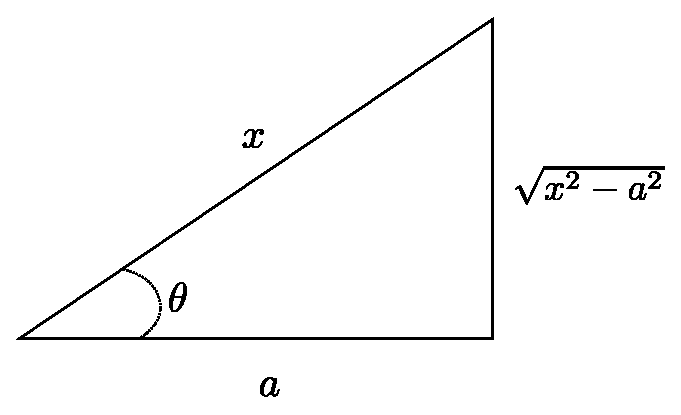
\includegraphics[width=0.4\textwidth]{continuous/integration/asectheta.eps}
  \end{center}
\end{figure}
For integrands with $\sqrt{a^2-x^2}$, let $x=a \sin \theta$ and $\ud x = a \cos \theta \ud \theta$.
\begin{figure}[H]
  \begin{center}
    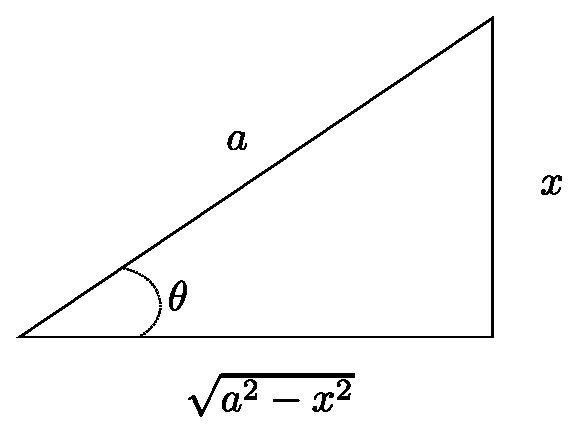
\includegraphics[width=0.4\textwidth]{continuous/integration/asintheta.eps}
  \end{center}
\end{figure}
For integrands with $ \sqrt{x^2+a^2}$, let $x = a \tan \theta$ and $\ud x = \sec^2 \theta \ud \theta$.
\begin{figure}[H]
  \begin{center}
    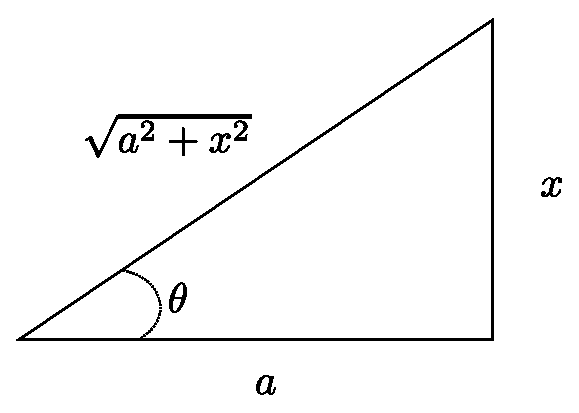
\includegraphics[width=0.4\textwidth]{continuous/integration/atantheta.eps}
  \end{center}
\end{figure}

\begin{ex}
  Integrate
  \[ \int \frac{\ud x}{x \sqrt {x^2 -4}} \]
  \begin{sol}
    Let $x=2 \sec \theta$ and $\ud x = 2 \sec \theta \tan \theta \ud \theta$.
    \begin{align*}
      \int \frac{\ud x}{x \sqrt {x^2 -4}}
      &= \int \frac{2 \sec \theta \tan \theta \ud \theta}{2 \sec \theta \sqrt{4\sec^2 \theta -4}} \\
      &= \int\frac{tan \theta \ud \theta}{\sqrt{4 \sec^2 \theta -4}} \\
      \intertext{Now we use the trigonometric identity $1+\tan^2\theta=\sec^2\theta$.}
      &= \int \frac{\tan\theta\ud\theta}{\sqrt{4(1+\tan^2\theta)-4}}\\
      &= \int \frac{\tan\theta\ud\theta}{\sqrt{4\tan^2\theta}}\\
      &= \int\frac{\tan\theta\ud\theta}{2\tan\theta}\\
      &= \int \frac{1}{2}\ud\theta \\
      &= \frac{1}{2}\theta+C\\
      \intertext{Now we draw a triangle, using the numbers from our original substitution:}
      % add a picture
      &=\frac{1}{2}\arcsec{\frac{x}{2}} +C
    \end{align*}
    \begin{figure}[H]
      \begin{center}
        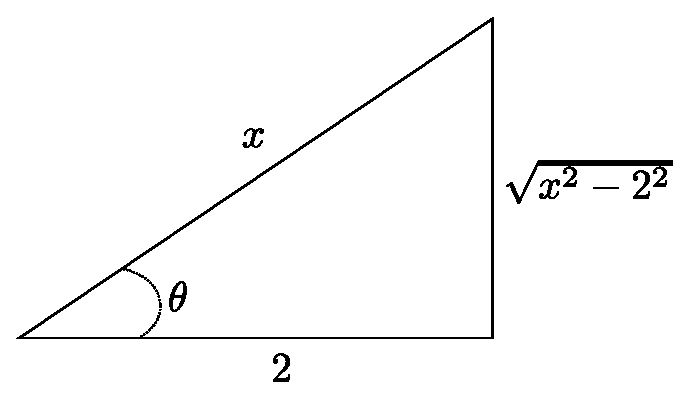
\includegraphics[width=0.4\textwidth]{continuous/integration/secexample.eps}
      \end{center}
    \end{figure}
  \end{sol}
\end{ex}
% \begin{ex}
%   \[ \int \frac{dx} {x \sqrt{x^{2}-4}} \]
%   \begin{sol}
%   \begin{align*}
%     \lets x&=2\sec \theta & \lets dx &= 2 \sec \theta \tan \theta \ud \theta
%   \end{align*}
%   \begin{align*}
% 	  \int \frac{\ud x} {x \sqrt{x^2-4}}
% 	  =&\int \frac{2 \sec \theta \tan \theta \ud \theta}{2 \sec \theta \sqrt{4\sec^2\theta-4}} \\
% 	  =&\int \frac{\tan \theta \ud \theta}{\sqrt{4\sec^2 \theta-4}} \\
% 	  =&\int \frac{\tan \theta}{2 \tan \theta} \ud \theta
% 	  = \frac {1}{2} \theta + C \\
%   \end{align*}
% This is unfinished, we still need to solve for $\theta$.
% \end{sol}
% \end{ex}
\begin{ex}
  \[ \int \frac{\ud x}{\sqrt{1-x^{2}}} = \sin^{-1}x+C \]
\end{ex}
\begin{ex}
  \[ \int \frac{2x}{\sqrt{1-x^2}}dx \]
  \begin{sol}

  \[ \text{let} u = 1-x^{2} \ldots \]
\end{sol}
\end{ex}
\begin{ex}
  \[ \int x^{3} \sqrt {4-x^2} \ud x \]
  \begin{sol} Although perhaps solvable using integration by parts, we will use trigonometric substitution.
  \begin{align*}
    \lets  x &= 2 \sin{\theta} \\ \lets \ud x &= 2\cos \theta \ud \theta
  \end{align*}
  \begin{align*}
    \int x^{3} \sqrt {4-x^2} \ud x
    =&\int 8\sin^3 \theta \, 2\cos\theta \, 2\cos\theta \, \ud\theta
   =32 \int \sin^{3}\theta\cos^{2} \theta \ud\theta \\
   =& 32 \int \sin^{2}\theta\cos^{2} \theta\sin \theta \ud\theta \\
   =& 32 \int (1-\cos^{2}\theta) \cos^{2} \theta\sin \theta \ud\theta \\
   \intertext{Let $u=\cos\theta$ and $\ud u = -\sin \theta \ud \theta$.}
   =&-32 \int (1-u^{2})\,u^{2}\ud u \\
   =&\frac {-32u^3}{3}+\frac{32u^5}{5}+C \\
   =&\frac{-32\cos^{2}\theta}{3}+\frac{32\cos^{5}\theta}{5}+C \\
   =&\frac {-32}{3} \left(\frac{\sqrt{4-x^2}}{2}\right)+\frac {32}{5} \left(\frac{\sqrt{4-x^2}}{2}\right)^5+C \\
 \end{align*}
 \end{sol}
\end{ex}

% \begin{homework}
%   Read Section 8.3.
% \end{homework}

\begin{ex}
  \[ \int \sqrt{x^2+6x} \ud x \]
  \begin{sol}
    \begin{align*}
      \int \sqrt{x^2+6x} \ud x =&\int \sqrt{x^2+6x+9-9}\ud x
      =\int \sqrt{(x+3)^2-9}\ud x \\
      \intertext{Now let $x+3=3\sec\theta$ and $\ud x=3\sec\theta \tan\theta \ud\theta$.}
      =& 3 \int \sqrt{9\sec^2\theta-9}\sec\theta \tan\theta \ud \theta \\
      =& 9 \int \tan^2\theta\sec\theta\ud\theta
  \end{align*}
\end{sol}
\end{ex}
\begin{ex}
  Integrate
    \[ \int \frac{1}{\sqrt{x^2+2x+5}}\ud x \]
  \begin{sol}
    \begin{align*}
      \int \frac{1}{\sqrt{x^2+2x+5}}\ud x
      =& \int \frac{1}{\sqrt{x^2+2x+1+4}} \\
      =& \int \frac{1}{\sqrt{(x+1)^2+4}} \\
      \intertext{Let $u=x+1$ and $\ud u=\ud x$.}
      =& \int \frac{\ud u}{\sqrt{u^2+4}} \\
      =& \arcsin \frac{x+1}{4}+C
    \end{align*}
  \end{sol}
\end{ex}


\section{Partial Fraction Decomposition}

A rational function $P(x)/Q(x)$ can be rewritten using what is known as partial fraction decomposition. This procedure often allows integration to be performed on each term separately by inspection. For each factor of $Q(x)$ the form $(a\,x+b)^m$:

\begin{equation}
  \frac{A_1}{a\,x+b}+\frac{A_2}{(a\,x+b)^2}+\ldots+\frac{A_m}{(a\,x+b)^m}
\end{equation}

For each factor of the form $(a\,x^2+b\,x+c)^m$ introduce terms:

\begin{equation}
  \frac{A_1\,x+B_1}{a\,x^2+b\,x+c}+\frac{A_2\,x+B_2}{(a\,x^2+b\,x+c)^2}+\ldots+\frac{A_m\,x+B_m}{(a\,x^2+b\,x+c)^m}
\end{equation}

Then write:

\begin{equation}
  \frac{P(x)}{Q(x)}=\frac{A_1}{a\,x+b}+\ldots+\frac{A_2\,x+B_2}{(a\,x^2+b\,x+c)^2}+\ldots
\end{equation}

And solve for $A_i$s and $B_i$s.


\subsection{Repeated Linear/Quadratic Den. Factors}

\begin{align*}
  \frac {\cdots}{\underbrace{(x^2+3)^2}_\text{quadratic} \, \underbrace{(x+1)}_\text{linear} \, \underbrace{(x^2+x+4)}_\text{quadratic}}
  &=\frac {Ax+B}{(x^2+3)^2} + \frac{Cx+D}{(x^2+3)^1} + \frac {E}{x+1} + \frac {Fx+G}{x^2+x+4}
\end{align*}

\begin{align*}
  \frac {\cdots}{(x^2-2x+1)(x^2-4x+4)}
  &=\frac {\cdots}{(x-1)^2(x-2)^2} \\
  &=\frac{A}{(x-1)^2}+\frac{B}{x-1}+\frac{C}{(x-2)^2}+\frac{D}{x-2}
\end{align*}

\subsection{Determining A,B,C, \dots}

Multiply the denominator by both sides of the new equation:
\[ {denominator}*\left[\frac{x^3+2x^2+x+8}{(x^2+4)^2}\right]=\left[\frac{Ax+B}{(x^2+4)^2}+\frac{Cx+D}{(x^2+4)^1}\right]*{denominator} \]

Now solve for \(A\), \(B\), and \(C\).

\begin{align*}
  x^3+2x^2+x+8 &= (Ax+B)+\,(Cx+D)(x^2+4)\\
  x^3+2x^2+x+8 &= (Ax+B)+Cx^3+4Cx+Dx^2+4D
\end{align*}

Now:
\begin{table}[H]
  \centering
  \begin{tabular}{r|l}
    \(x^2\) terms & \( 2=D \) \\
    \(x\) terms & \( 1 = A + 4C  \) \\
    const terms & \( 8 = B + 4D \)
  \end{tabular}
\end{table}

\subsection{Factoring}

\begin{equation}
  (F)^3+(L)^3=(F+L)(F^2-FL+L^2)
\end{equation}
\begin{equation}
  (F)^3-(L)^3=(F-L)(F^2+FL+L^2)
\end{equation}
Note: you cannot factor a sum of perfect squares.
\begin{remark} When factoring quadratics, consider the discriminant (from the quadratic formula at \ref{app:eq:quadratic}):
  \begin{align*}
    &10x^2-x-2 \\
    &b^2-4ac \\
    &(-1)^2-4(10)(-2)
  \end{align*}
\end{remark}

% \begin{homework} From \emph{Thomas' Calculus}, solve
%
%   \begin{tabular}{llr}
%     page & problems & sols \\ \hline
%     475 & 25 \\ & 27 (b) \\ & 32 \\
%     492 & 70 & $\frac{-x^2}{2}-\frac{3}{2}\ln{|x+2|}-\frac{5}{2}ln{|x-2|}$ \\
%     & 72 & ($\sin^1{x+1}$) \\
%     & 75 \\
%     & 75 & $\frac{x^2}{2}+2x+3ln{|x-1|}-\frac{1}{x-1}$ \\
%     & 79 \\ &83\\&85\\&86&$\frac{x^2-1}{2}e^{x^2}$\\&87\\&88&$\frac{-\tan^{-1}x}{x}+\ln{|x|}-\ln{\sqrt{|1+x^2}|}$\\&99\\&101\\
%   \end{tabular}
% \end{homework}


% \section{Test Review}
% \begin{comment}
% \begin{ex}
%   $$ \int cot^3 (2x)\ud x $$
%   $$ \int (csc^2 2x -1) \, cot2x \ud x $$
%   $$ \int csc^2 2x\, cot \, 2x \ud x - \int \frac {cos\,2x}{sin\,2x}\ud x $$
%   $$ \text {abandoned ...} $$
% \end{ex}
% \end{comment}
% %\begin{ex}
% %  Integrate \[ \int \sqrt{16-9x^2} \ud x \]
% %  \begin{sol}
% %  Factor out a $9$.
% %  \begin{align*}
% %    \int \sqrt{16-9x^2} \ud x
% %    =& \int \sqrt{9\left(\frac{16}{9}-x^2\right)} \ud x
% %    =3 \int \sqrt{\frac{16}{9}-x^2} \ud x \\
% %    \intertext{Let $x= \frac{4}{3}\sin \theta$ and $\ud x = \frac{4}{3}\cos \theta \ud \theta$.}
% %    =& 3 \int \sqrt{\frac{16}{9}-\left( \frac{4}{3}\sin\theta \right)^2}\,\frac{4}{3}\cos\theta\ud\theta \\
% %    =& 3 \int \sqrt{\frac{16}{9}-\frac{16}{9}\sin^2\theta}\,\frac{4}{3}\cos\theta\ud\theta \\
% %    =& 3 \int \frac{4}{3}\sqrt{1-\sin^2 \theta} \,\frac{4}{3}\cos\theta\ud\theta \\
% %    =& \frac{16}{3} \int \sqrt{\cos^2\theta}\cos\theta\ud\theta \\
% %    =& \frac{16}{3} \int \cos^2\theta\ud\theta
% %  \end{align*}
% %  \center{[Incomplete. See comments for details.]}
% %\end{sol}
% %\end{ex}
% %\begin{ex}
% %  $$ \int \sqrt{16-9x^2} \ud x $$
% %  $$ \int \sqrt{9\frac{16}{9}-x^2}\ud x $$
% %  $$ \text {try } x = \frac{4}{3}\sin \, \theta $$
% %  $$ dx = \frac{4}{3}cos\,\theta \, \ud \theta $$
% %  $$ 3 \int \sqrt{\frac{16}{9}-x^2}\ud x $$
% %  $$ 3 \int \sqrt{\frac{16}{9}-\frac{16}{9}sin^2 \, \theta } \, \frac{4}{3}cos\,\theta \, d\theta $$
% %  $$ 3 \int \frac {4}{3} \sqrt{cos^2 \, \theta } \frac{4}{3} cos\,\theta\,d\theta $$
% %  $$ \frac{16}{3} \int cos^2 \theta \, d \theta $$
% %  $$ \frac{16}{3}\left[\frac{\theta}{2}+\frac{sin\,2\theta}{4}\right] $$
% %  $$ \theta = sin^{-1}\,\frac{3x}{4} $$
% %  $$ \frac{16}{3}\left[\frac{sin^{-1}\,\frac{3x}{4}}{2}+\frac{sin\,2(sin^{-1}\,\frac{3x}{4})}{4}\right] $$
% %\end{ex}

\subsection{Examples}

\begin{ex}
  \begin{align*}
    \frac{x+3}{x^2-3x+2}
   =&\frac{x+3}{(x-2)(x-1)} \\
   =&\frac{A}{x-2}+\frac {B}{x-1}
  \end{align*}
\end{ex}
\begin{ex}
  \begin{align*}
    \frac {x+3} {x^4+3x^3+6x^2+12x+8}
    =&\frac {x+3} {(x^2+4)(x+1)(x+2)} \\
    =&\frac{A}{x+1}+\frac{b}{x+2}+\frac{Cx+D}{x^2+4}
  \end{align*}
\end{ex}
\begin{ex}
  \begin{align*}
    \frac{x+3}{x^4+5x^2+4}
    =&\frac{x+3}{(x^2+4)(x^2+1)}\\
    =&\frac{Ax+B}{x^2+4}+\frac{Cx+D}{x^2+1}
  \end{align*}
\end{ex}
\begin{ex}
  \begin{align*}
    \frac{1}{x^2-1}
    =&\frac{1}{(x-1)(x-1)} \\
    =&\frac{A}{x+1}+\frac{B}{x-1}
  \end{align*}
\end{ex}
\begin{ex}
  \begin{align*}
    \frac{1}{x^2-x}
     =&\frac{1}{x(x-1)} \\
     =&\frac{A}{x}+\frac{B}{x-1}
  \end{align*}
\end{ex}

\begin{ex}
  \begin{align*}
   \frac {9x^2+7x-4}{x^3-3x^2-4x} \\
   \frac {9x^2+7x-4}{x(x^2-3x-4)} \\
   \frac {9x^2+7x-4}{x(x-4)(x+1)} \\
   \frac{A}{x}+\frac{B}{x-4}+\frac{C}{x+1}
  \end{align*}
\end{ex}
\begin{ex}
  \begin{align*}
   \frac {x+3}{x^2-4} \neq \frac {A}{x+2} + \frac {B}{x-2} \\
   \frac {x+3}{x^2-4} = \frac {x^3+0x^2+0x+4}{x^2-4} \\
   \frac {x+3}{x^2-4} = x + \underbrace{\frac {4x+4}{x^2-4}}_{\frac{A}{x+2}+\frac{B}{x-2}}
 \end{align*}
\end{ex}
\begin{ex}
  \[ \int \frac{8x^4+6x^2-3x+1}{2x^2-x+2} \]
  \begin{sol}
  Use long division to simplify as follows:
    \begin{center}
      \polylongdiv{8x^4+6x^2-3x+1}{2x^2-x+2}
    \end{center}
    \begin{align*}
      \frac{8x^4+6x^2-3x+1}{2x^2-x+2} &=
      4x^2+2x+\frac{\overbrace{-7x+1}^{Ax+B}}{2x^2-x+2}
    \end{align*}
    So
    \begin{align*}
      \int \frac{8x^4+6x^2-3x+1}{2x^2-x+2}
      &= \int 4x^2+2x+\frac{-7x+1}{2x^2-x+2}
    \end{align*}
    Then solve.
  \end{sol}
\end{ex}
\begin{ex}
  \[ \int \frac{dx}{x^2+2x} \]
  \begin{sol}
    Note that
    \[ \left[ \frac{1}{x^2+2x}\right] \text{ is }
    \left[\frac{A}{x}+\frac{B}{x+2}\right] \]
    \begin{align*}
      \int \frac{\ud x}{x^2+2x} &=
      \int \frac{\frac{1}{2}}{x}+\frac{\frac{1}{2}}{x+2} \ud x \\
      &= \int \frac{\frac{1}{2}}{x} \ud x+\int\frac{\frac{1}{2}}{x+2} \ud x \\
      &= \frac{1}{2}\ln{|x|}+\frac{-1}{2}\int\frac{\ud u}{u} \\
      &= \frac{1}{2}\ln{|x|}+\ln{|x+2|}
    \end{align*}
  \end{sol}
\end{ex}

\begin{ex}
  Write the partial fraction decomposition of
  \[ \frac{1}{x^4+2x^2+1} \]
  \begin{sol}
    It's a trinomial, so we know we have to try binomial times binomial--and that works.
    \begin{align*}
	    \frac{1}{x^4+2x^2+1}
	      &=\frac{1}{(x^2+1)(x^2+1)}
	       =\frac{Ax+B}{(x^2+1)^2}+\frac{Cx+D}{x^2+1}
	    \intertext{Multiply both sides by the denominator}
	      &=Ax+B+(x^2+1)(Cx+D)
    \end{align*}
    Now, solve for A, B, C, and D.
    \begin{align*}
      1&=Ax+B+(x^2+1)(Cx+D) \\
      1&=B+D \\
      0&=A+C \\
      0&=C \\
      0&=D
    \end{align*}
    So A is 0, B is 1, C is 0, and D is 0.
  \end{sol}
\end{ex}
%\subsection{Integrals}
%$$\int \frac{dx}{x^2-16} $$
%$$ (x^2-16)*\left[\frac{1}{(x+4)(x-4)}\right=\left[\frac{A}{(x+4)}+\frac{B}{x-4}\right]*(x^2-16) $$
%$$ 1 = A(x-4)+B(x+4) $$
\begin{ex}
  Integrate
  \[ \int \frac{1}{(x+1)(x-1)} \]

  \begin{sol}
  \begin{align*}
    \int \frac{1}{(x+1)(x-1)}
      =& \int \frac{A}{x+1}+\frac{B}{x-1}\ud x \\
    \intertext{Solve for $A$ and $B$.}
      =& \int \frac{-1/2}{x+1}+\frac{1/2}{x-1} \\
      =& \frac{-1}{2} \int \frac{\ud x}{x+1}
         + \frac{1}{2} \int \frac{\ud x}{x-1}
  \end{align*}
\end{sol}
\end{ex}
\begin{ex}
  Integrate
  \[ \int \frac{x^2}{x+8} \ud x \]
  \begin{sol}
    Use long division to simplify the integrand:
    \begin{center}
      \polylongdiv{x^2+0x+0}{x+8}
    \end{center}
      \begin{align*}
        \int \frac{x^2}{x+8} \ud x
        =&\int x-8 + \frac{64}{x-8}\ud x\\
        =&\frac{1}{2}x^2-8x+64\ln{|x+8|}+C
      \end{align*}
  \end{sol}
\end{ex}
\begin{ex}
  Integrate
  \[ \int \frac{1}{x^2-5x-6}\ud x \]
  \begin{sol}
    Use partial fraction decomposition:
    \begin{align*}
    \frac{1}{x^2-5x-6} = \frac{1}{(x-6)(x+1)}\\
    \frac{1}{(x-6)(x+1)} = \frac{A}{x-6}+\frac{B}{x+1} \\
    1 = A(x+1)+B(x-6) \\
    1 = Ax+A+Bx-6B \\
    1 = Ax+Bx+A-6B \\
    \end{align*}
    If $x=0$, then $A-6B=1$. If $x=1$, then $2A-5B=1$. We can substitute the first equation into the second to get
    \begin{align*}
      2(1+6B)-5B&=1 \\
      2+12B-5B&=1 \\
      B&=-1/7 \\
    \end{align*}
    \begin{align*}
      A-6B&=1 \\
      A-6(1/7)&=1 \\
      A&=1/7 \\
    \end{align*}
    \begin{align*}
      \frac{1}{x^2-5x-6}=&\frac{1/7}{x-6}-\frac{1/7}{x+1} \\
      \int \frac{1}{x^2-5x-6}\ud x=&\int  \frac {1/7}{x-6}-\frac{1/7}{x+1} \ud x \\
      =& \frac{1}{7} \int \frac{1}{x-6}-\frac{1}{x+1}\ud x \\
      =& \frac{1}{7}\left(\ln{|x-6|}-\ln{|x+1|}\right)+C
    \end{align*}
  \end{sol}
\end{ex}
\section{Simpson's Rule}
\begin{ex}
  Estimate
  \[ \int^5_1 \frac{1}{x}\ud x \]
  using the trapezoidal rule with four trapezoids.
  \begin{remark}
    For one trapezoid:
      \[ \frac{\Delta x}{2}(y_0+y_1) \]
    For the entire Trapezoid Rule:
      \[ \frac{\Delta x}{2}(y_0+2y_1+2y_2+2y_3+\dots+y_n) \]
    For full-blown Simpson's Rule:
      \[ \frac{\Delta x}{3}(y_0+4y_1+2y_2+4y_3+ \dots +2y_{n-2}+ 4y_{n-1}+y_n) \]
  \end{remark}
  \begin{remark}
    The question might be seen as: ``\dots using the trapezoidal rule with $n=4$.''
  \end{remark}
  \begin{sol}
  \begin{align*}
    \int^5_1 \frac{1}{x}\ud x
      \approx & \frac{\overbrace{\Delta x}^1}{2}
        \left(\frac{1}{1}+2 \frac{1}{2}+2 \frac{1}{3}+ 2 \frac{1}{4}+1 \frac{1}{5}\right)
        \\
      =& \frac{1}{2}(2^{1/2}+2/3+1/5) \\
      =& \frac{1}{2}(5/2+13/15) \\
      =& \frac{101}{60}
  \end{align*}
\end{sol}
\end{ex}
\begin{ex}
  Estimate
  \[ \int^5_1 \frac{1}{x}\ud x \]
  using Simpson's Rule with $n=8$.

  \begin{sol}
  \begin{align*}
  \int^5_1 \frac{1}{x}\ud x
   \approx & \frac{\overbrace{\Delta x}^{1/2}}{3}
     \left(\frac{1}{1}+4 \frac{1}{3/2}+2 \frac{1}{2} + 4 \frac{1}{5/2}+ \dots \right)
  \end{align*}
  Not a real problem, so not finished.
\end{sol}
\end{ex}


\section{Improper Integrals}

\begin{defn}
\emph{Improper integrals} occur in cases where you are integrating across an infinite domain or infinite range.
\end{defn}

\begin{figure}[H]
  \begin{center}
    \begin{tikzpicture}
      \begin{axis}[
        ylabel={$\frac{1}{\sqrt{x}}$},
        axis x line=bottom,
        axis y line=center,
        tick align=outside,
        axis y discontinuity=crunch,
        xtickmax=10,
        ytickmin=10,
        ]
        \addplot {1/sqrt(x)};
      \end{axis}
    \end{tikzpicture}
  \end{center}
  \caption{An example of a function that can produce improper integrals.}
\end{figure}


\subsection{Infinite Range}

\begin{ex}
	\[ \int^{9}_1 \frac{1}{x-4}\ud x \]
	Right and left approach problem spot.
\end{ex}
\begin{ex}
	\[ \int^{39}_{4}\frac{1}{\sqrt{x-4}}\ud x \]
	Right approach problem spot.
\end{ex}
\begin{ex}
	\[ \int^0_{-4} \ln{|x|} \ud x \]
	Left approach problem spot.
\end{ex}
\begin{ex}
  \[ \int^{10 \pi}_{-6\pi} \sec x \ud x \]
  Problems with right and left approach.
\end{ex}
\begin{ex}
This is considered a ``Classic.''
  \begin{align*}
    &\int^{b}_{a} \frac{1}{(b-x)^p} \ud x && \text{and} &&\int^{b}_{a} \frac{1}{(x-a)^p} \ud x
  \end{align*}
\end{ex}
\begin{ex}
  Integrate:
    \[ \int^{-2}_{-6} \frac{1}{(x+6)^1} \ud x \]
  \begin{sol}
    \begin{align*}
      \int^{-2}_t \frac{1}{x+6} \ud x
      =& \ln{|x+6|}\bigg|^{-2}_t \\
      =& \lim_{t \to -6^+} \ln{|-2+6|}-\underbrace{\ln{|-6^++6|}}_\text{Diverges.}
    \end{align*}
  \end{sol}
\end{ex}
\begin{ex}
  Integrate:
    \[ \int^{6}_{2} \frac{1}{(x-6)^2} \ud x \]
  \begin{sol}
  \begin{align*}
    \int^{t}_2 \frac{1}{x+6} \ud x
    =& \frac{(x-6)^{-1}}{-1} \bigg|^t_2 \\
    =& \lim{t \to 6^-} \frac{(t-6)^{-1}}{-1}-\frac{(2-6)^{-1}}{-1}
  \end{align*}
\end{sol}
\end{ex}
\begin{ex}
  Integrate:
  \begin{align*}
    \int^{3}_{1} \frac{1}{\sqrt{x-1}}
    =& \frac{(x-1)^{1/2}}{1/2}\bigg|^3_t \\
    =& \lim_{t \to 1+} \frac{(3-1)^{1/2}}{1/2}-\frac{(t-1)^{1/2}}{1/2}
  \end{align*}
\end{ex}
\begin{ex}
  Integrate.
  \[ \int^{39}_4 \frac{1}{\sqrt{x-4}} \ud x \]
  Substitute with $4 \to t$:
  \[ \int^{39}_t \frac{1}{\sqrt{x-4}} \ud x \]
  And evaluate:
  \begin{align*}
    \int^{39}_t \frac{1}{\sqrt{x-4}} \ud x
    =& \lim_{t \to 4^+} \frac{(x-4)^{1/2}}{1/2} \bigg|^{39}_t \\
    =& \lim_{t \to 4^+} \frac{(39-4)^{1/2}}{1/2}-\frac{(t-4)^{1/2}}{1/2} \\
    =& \frac{(39-4)^{1/2}}{1/2}
  \end{align*}
\end{ex}
\begin{ex}
  Integrate.
  \[ \int^{29}_1 \frac{1}{x-4} \ud x \]
  \begin{sol}
    Substitute $29 \to t$:
    \begin{align*}
      \int^{29}_1 \frac{1}{x-4} \ud x =& \int^t_1 \frac{1}{x-4} \ud x
      + \int^{29}_t \frac{1}{x-4} \ud x \\
      &= \ln{|x-4|}\bigg|^t_1 + \ln{|x-4|} \bigg|^{29}_t \\
      &=\ln{|t-4|}-\ln{|1-4|}+\ln{|29-4|}-\ln{|t-4|} \\
      &=\lim_{t \to 4^-} \left[\underbrace{\ln{|t-4|}}_{\frac{1}{-\infty}}-\ln{|1-4|}\right]+\lim_{t \to 4^+} \left[\ln{|29-4|}-\underbrace{\ln{|t-4|}}_{\frac{1}{\infty}}\right]
    \end{align*}
    Diverges.
  \end{sol}
\end{ex}
\begin{ex}
  Integrate:
  \[ \int^5_0 \ln{x} \ud x \]
  \begin{sol}
  \begin{align*}
    \int^5_t \ln{x} \ud x =&x \ln{x} -x \bigg|^5_t \\
    &=5 \ln{5} -5-t\ln{t}+t \\
    \intertext{Now evaluate the limit as:}
    \int^5_0 \ln{x} \ud x =& \lim_{t \to 0^+}5 \ln{5} -5-t\ln{t}+t \\
    &=5 \ln 5 - 5
  \end{align*}
\end{sol}
\end{ex}

% \begin{homework}
%   4th online homework assignment due SUNDAY at end of break.
%
%   Read section 8.7.
%
%   pg. 487 \#3, 4 (4), 5, 6, ($\frac{-9}{2}$), 7, 8 (1000), 15, 25, 26 (1)
% \end{homework}

\subsection{Infinite Domain}

For these, the integrand is well behaved throughout the integration interval. The problem is that we are integrating across an interval $[a, b]$ where either $a$ or $b$ is $\infty$ or $-\infty$.

\begin{equation}
  \int^{\infty}_{\#} f(x) \ud x
\end{equation}
We would treat this an indefinite integral:
\[ \int f(x) \ud x = F(x) \]
Then evaluate it as follows:
\[ \lim_{t \to \infty} F(x)\bigg|^{t}_{\#} \] \\

\begin{equation}
  \int^{\#}_{-\infty} f(x) \ud x
\end{equation}
Like the first one, we would treat this as an indefinite integral:
\[ \int f(x) \ud x = F(x) \]
Then evaluate it as follows:
\[ \lim_{t \to \infty} F(x)\bigg|^{\#}_{-\infty} \] \\

Others, still, look like this:
\begin{equation}
  \int^{\infty}_{-\infty} f(x) \ud x
\end{equation}
Treat this as a combination of two of the above integrals. Rewrite it as:
\[ \int^{a}_{-\infty} f(x) \ud x
    + \int^{\infty}_{a} f(x) \ud x \]
choosing some arbitrary \(a\), which we usually choose to be \(0\).

\begin{ex}
    For $p>1$, does the following integral converge or diverge?
    \[ \int^\infty_1 \frac{1}{x^p} \ud x \]
    \begin{sol}
      The integral converges.
    \end{sol}
  \end{ex}
\begin{ex}
	\[ \int^{\infty}_1 x^{-3} \ud x \]
	\begin{sol}
	\begin{align*}
		\int^{\infty}_1 x^{-3} \ud x &=\lim_{t \to \infty} \frac{x^{-2}}{2}\bigg|^{t}_{1} \\
		  &=\lim_{t \to \infty} \frac{t^{-2}}{-2}-\frac{1^{-2}}{-2} \\
		  &=\lim_{t \to \infty} \frac{1}{-2t^2}+\frac{1}{2}
	\end{align*}
The integral converges to $1/2$.
\end{sol}
\end{ex}
\begin{ex}
	\[ \int^\infty_1 \frac{1}{\sqrt{x}}\ud x \]
	\begin{sol}
	\begin{align*}
		\int^\infty_1 \frac{1}{\sqrt{x}}\ud x &=\lim_{t \to \infty} \frac{x^{1/2}}{\frac{1}{2}}\bigg|^t_1 \\
		&=\lim_{t \to \infty} \frac{t^{1/2}}{\frac{1}{2}}-\frac{1^{1/2}}{\frac{1}{2}} \\
		&=\lim_{t \to \infty} 2t^{1/2}-2
	\end{align*}
The integral diverges.
\end{sol}
\end{ex}
\begin{ex}
	\[ \int^\infty_0 \frac{1}{x^2+1} \]
	\begin{sol}
	\begin{align*}
		\int^\infty_0 \frac{1}{x^2+1} &= \lim_{t \to \infty} \arctan x \bigg|^t_0 = \lim_{t \to \infty} \arctan t - \arctan 0 \\
		&= \lim_{t \to \infty} \arctan t \\
		&= \lim_{t \to \infty} \arctan t \\
		&= \frac{\pi}{2}
	\end{align*}
  \begin{figure}[H]
    \begin{center}
        \subfigure[\(f(x)=\tan{x}\).]{
          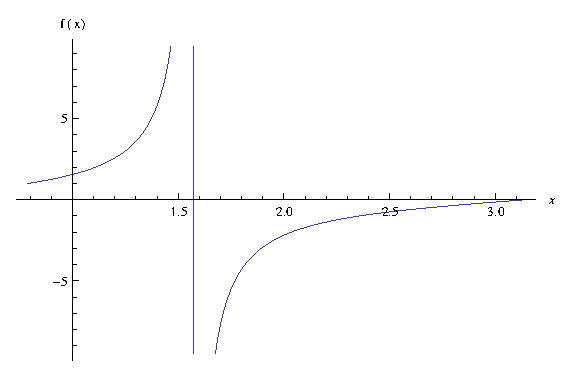
\includegraphics[scale=0.8]{graphs/tanx.eps}
        }
        \subfigure[\(f(x)=\arctan{x}\).]{
          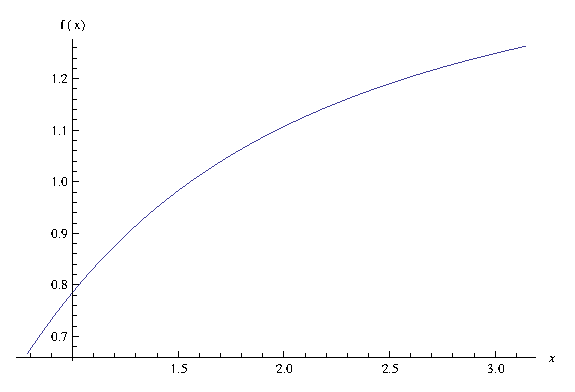
\includegraphics[scale=0.8]{graphs/arctanx.eps}
        }
    \end{center}
    \caption{\(\tan x\) compared with \(\arctan x\).}
  \end{figure}
  \end{sol}
\end{ex}
\begin{ex}
	\[ \int^0_{-\infty} \frac{x^2}{x^3-1} \]
	\begin{remark}
	  If $0 \to 1$, this would be a Type I integral.
	\end{remark}
	\begin{sol}
	  \begin{align*}
	  	\int^0_{-\infty} \frac{x^2}{x^3-1} &=\int^0_{-\infty} \frac{1}{3} \frac{\ud u}{u} \\
	  	&= \lim_{t \to \infty} \frac{1}{3}\ln{|x^3-1|\bigg|^0_t}
	  	= \lim_{t \to \infty} \frac{1}{3} \ln{|-1|}-\frac{1}{3}\ln{|t^3-1|} \\
	  	&= \lim_{t \to \infty} \frac{1}{3}ln{1}-\frac{1}{3}\ln{|t^3-1|} \\
	  	&= \lim_{t \to \infty} -\frac{1}{3}\ln{|t^3-1|}
	  \end{align*}
    The integral diverges.
  \end{sol}
\end{ex}
\begin{ex}
	\[ \int^0_{-\infty} e^x \ud u \]
	\begin{remark}
	  This is likely to converge, because of the $e^{-\infty}$.
	\end{remark}
	\begin{sol}
	\begin{align*}
		\int^0_{-\infty} e^x \ud u & =\lim_{t \to -\infty} e^x \bigg|^0_t \\
		&=\lim_{t \to -\infty} e^0-e^t
	\end{align*}
	The integral converges to $1$.
  \end{sol}
\end{ex}
\begin{ex}
	\[ \int^\infty_{-\infty} e^{-x} \cos x \ud x \]
	\begin{sol}
  First, break this into two parts.
	\begin{align*}
		\int^\infty_{-\infty} e^{-x} \cos x \ud x
		&=\int^0_{-\infty} e^{-x} \cos x \ud x+\int^\infty_0 e^{-x} \cos x \ud x \\
		\intertext{Then, treat it as an indefinite integral and evaluate using integration by parts:}
		\int e^{-x} \cos x \ud x&=\frac{e^{-x}\sin x - e^{-x} \cos x}{2}
		\intertext{Now, return to our original function.}
		\lim_{t \to \infty} e^{-x} \cos x \ud x
		&=\lim_{t \to \infty}
		  \frac{e^{-x}\sin x - e^{-x} \cos x}{2}\bigg|^0_t
		  -\frac{e^{-x}\sin x - e^{-x} \cos x}{2}\bigg|^t_0 \\
		&=\lim_{t \to \infty}
		  \left[\frac{e^{-0}\sin  - e^{-0} \cos 0}{2}
		  -\frac{e^{-t}\sin t - e^{-t} \cos t}{2}\right]
		  -\left[0+\frac{1}{2}\right] \\
	\end{align*}
	Because the left half of this diverges, the entire integral diverges.
\end{sol}
\end{ex}
\begin{ex}
  This is one of the classics:
	\[ \int^\infty_1 \frac{1}{x}\ud x \]
	\begin{sol}
	  Consider:
    \[ \int^\infty_1 \frac{1}{x^{1.000000001}}\ud x = x^{-0.000000001}\bigg|^\infty_1=0-\frac{1}{1^{0.000000001}}\]
    Therefore:
	  \begin{align*}
	  	\int^\infty_1 \frac{1}{x}\ud x
	  	&=\lim_{t \to \infty} \ln{|x|}\bigg|^t_1=\lim_{t \to \infty} \ln{|t|}-\ln{|1|} \\
	  	& =\lim_{t \to \infty} \ln{|t|}
	  \end{align*}
	  Diverges.
  \end{sol}
\end{ex}
\begin{ex}
  \[ \int^\infty_1 \frac{1}{x^2}\ud x =\lim_{t\to\infty}
    \frac{x^{-1}}{-1}\bigg|^t_1 \]
  This integral converges.
\end{ex}

\section{Test Review}

\begin{ex}
  \[\int \cot^2x \csc^4x \ud x \]
  \begin{sol}
    Set aside a $\csc^2x$.
    \begin{align*}
      \int \cot^2x \csc^4x \ud x
      =& \cot^2x \csc^2x \csc^2x \ud x
    \end{align*}
    Remembering our basic trig identity
    \[ \sin^2x + \cos^2x = 1\]
    we can divide through by $\sin^2x$ to get
    \[ 1+\cot^2x=\csc^2x \]
    and substitute that into our new integral
    \begin{align*}
      \int\cot^2x\csc^2x\csc^2x\ud x
      =& \int \cot^2x (1+\cot^2x)\csc^2x \ud x \\
      \intertext{Now we let $u=\cot x$ and $\ud u=\csc^2x \ud x$.}
      =&\int u^2(1+u^2)\ud u \\
      \intertext{which we can do.}
      =& \frac{u^3}{3}+\frac{u^5}{5}+C \\
      \intertext{Now replace our old $u$-substitutions}
      =& \frac{\cot^3x}{3}+\frac{\cot^5x}{5}+C
    \end{align*}
  \end{sol}
\end{ex}
\begin{ex}
  \[ \int \tan x \sec^4x \ud x \]
  \begin{sol}
    Set aside a $\sec^2x$
    \begin{align*}
      \int \tan x\sec^4x \ud x
      = \int \tan x \sec^2 x \sec^2 x \ud x
    \end{align*}
    Remembering our basic trig identity
    \[ \sin^2x + \cos^2x = 1\]
    we can divide through by $\cos^2x$ to get
    \[ \tan^2x+1=\sec^2x \]
    and substitute that into our new integral
    \begin{align*}
      \int \tan x \sec^2 x \sec^2 x \ud x
      =& \int \tan x (\tan^2x-1) \sec^2x \ud x \\
    \end{align*}
    Now let $u=\tan x$ and $\ud u = \sec^2x \ud x$
    \begin{align*}
      \int \tan x (\tan^2x-1) \sec^2x \ud x
      =& \int u (u^2-1) \ud u \\
      =& \frac{u^3}{3}-\frac{u^2}{2}+C \\
      =& \frac{\tan^3x}{3}-\frac{\tan^2x}{2} +C
    \end{align*}
  \end{sol}
\end{ex}
\begin{ex}
  \[ \int x^2 e^x \ud x \]
  \begin{sol}
    \begin{align*}
      \int x^2 e^x\ud x
      =& x^2 e^x-2\int x e^x \ud x \\
      =& x^2 e^x -2 \left( x e^x - \int e^x \ud x \right) \\
      =& x^2 e^x -2 x e^x +2x +C
    \end{align*}
  \end{sol}
\end{ex}
\begin{ex}
  \[ \int^4_2 \frac{1}{x-4}\ud x \]
  \begin{sol}
    \begin{align*}
      \int^4_2 \frac{1}{x-4}\ud x
      =& x\ln{|x-4|}\bigg|^t_2 \\
      =& \ln{|t-4|}-\ln{|-2|}
    \end{align*}
    Now we go back to the original integral
    \[
      \int^4_2 \frac{1}{x-4}\ud x
      = \lim_{t \to 4^-}\ln{|t-4|}-\ln 2
      \]
      Remembering the graph of \(\ln{|x|}\)
      \begin{figure}[H]
        \begin{center}
          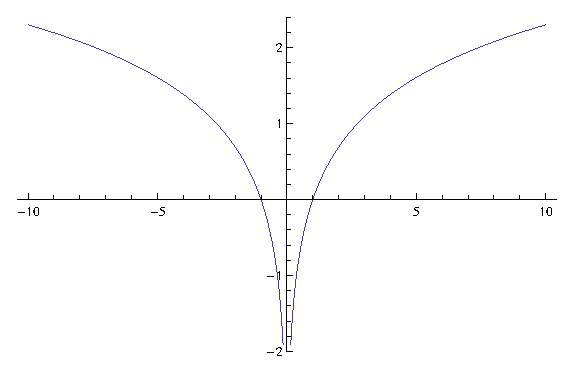
\includegraphics[scale=1]{graphs/logabsx.eps}
        \end{center}
        \caption{A plot of \(f(x)=\ln{|x|}\)}
      \end{figure}
      we can conclude that the integral diverges toward $-\infty$.
  \end{sol}
\end{ex}
\begin{ex}
  \[ \int^6_5 \frac{1}{(x-5)^{1/2}}\ud x \]
  \begin{sol}
    \begin{align*}
      \int^6_t \frac{1}{(x-5)^{1/2}}\ud x
      =& 2 \sqrt{x-5}\bigg|^6_t \\
      =& 2 \sqrt{6-5}-2\sqrt{t-5}
    \end{align*}
    \begin{align*}
      \int^6_5 \frac{1}{(x-5)^{1/2}}\ud x
      =& \lim_{t \to 5^+} 2\sqrt{6-5}-\underbrace{2\sqrt{t-5}}_{0} \\
      =& \lim_{t \to 5^+} 2\sqrt{6-5}\\
      =& 2
    \end{align*}
  \end{sol}
\end{ex}
\begin{ex}
  \[ \int^\infty_{\frac{8\sqrt 3}{3}}\frac{1}{x^2+64}\ud x \]
  \begin{sol}
    \begin{align*}
      \int \frac{1}{x^2-64}\ud x
      =& \int \frac{1}{64(\frac{x^2}{64}+1)} \\
      =&\frac{1}{8}\arctan{\frac{x}{8}} + C
    \end{align*}
    \begin{align*}
      \int^t_{\frac{8\sqrt 3}{3}}\frac{1}{x^2+64}\ud x
      =&\frac{1}{8}\arctan{\frac{x}{8}}\bigg|^t_{\frac{8\sqrt 3}{3}} \\
    \end{align*}
    \begin{align*}
      \int^\infty_{\frac{8\sqrt 3}{3}}\frac{1}{x^2+64}\ud x
      =& \lim_{t \to \infty} \frac{1}{8}\arctan{\frac{t}{8}}-\frac{1}{8}\arctan{\frac{\sqrt 3}{3}} \\
      =& \frac{1}{8}\left(\frac{\pi}{2}-\frac{\pi}{6}\right) \\
      =& \frac{\pi}{24}
    \end{align*}
  \end{sol}
\end{ex}
\begin{ex}
  \[\int x^3 \cos{3x} \ud x\]
  \begin{sol}
    We use integration by parts.
    \begin{align*}
      \int x^3 \cos{3x} \ud x
      =& \frac{1}{3}x^3\sin{3x}-\int x^2 \sin{3x}\ud x \\
      =& \frac{1}{3}x^3\sin{3x}-\left[
        \frac{-1}{3}x^2\cos{3x}+\frac{2}{3}\int x \cos{3x} \ud x
        \right] \\
        =& \frac{1}{3}x^3\sin{3x}+\frac{1}{3}x^2\cos{3x}-\frac{2}{3}\left[\frac{1}{3}x\sin{3x}-\frac{1}{3}\int \sin{3x}\ud x\right] \\
        =&\frac{1}{3}x^3\sin{3x}+\frac{1}{3}x^2\cos{3x}-\frac{2}{9}x\sin{3x}-\frac{2}{27}\cos{3x}+C
    \end{align*}
  \end{sol} \end{ex}

% \begin{homework}
%   Chapter 8 test on Friday, March 16, 2012.
% \end{homework}



\chapter{Sequences}
\label{ch:sequences}

%\begin{quote}
%  \emph{``Sequences are fundamental to the study of infinite series and many
%  applications of mathematics.''}
%
%\hfill\cite[p.~532]{thomas}
%\end{quote}
A \textbf{sequence}\index{sequence} is an ordered list of numbers. They are mostly important because of their application to \textbf{series},
detailed in Chapter \ref{ch:series}.
\section{Representing a Sequence}
\begin{defn}
  A \textbf{sequence} is a list of numbers
  \[ a_1, a_2, a_3, \ldots, a_n, \ldots\]
  in a given order. This order is important: The sequence \(2, 4, 6, 8, \ldots\) is not the same as the sequence \(4, 2, 8, 6, \ldots\).
\end{defn}
When we write sequences like \(\{a_n\}\), we are talking about the entire
sequence. A sequence like this is described as ``starting at'' a certain \emph{index},
usually \(n=1\). In the context of the series we'll be using, they are normally infinite
in length.

We can also write sequences using rules that describe their
terms, as follows:

\begin{ex}
\[ a_n = \frac{n!}{2n!+1} \]
  We can write out a few terms of the sequence
  \[
    \left\{
      \frac{1}{3},\frac{2}{5},\frac{6}{13},\frac{24}{49},\frac{120}{241},
    \ldots \right\}
  \]
  and then plot them %(shown in figure \ref{fig:firstsequence})
  to get a feel that the
  sequence is getting closer and closer to a certain number: \[ \frac{1}{2}.\] We would
  thus describe this sequence as \emph{converging to} the number \( \frac{1}{2} \)
% BROKEN FIGURE
%  \begin{figure}[h]
%    \begin{center}
%      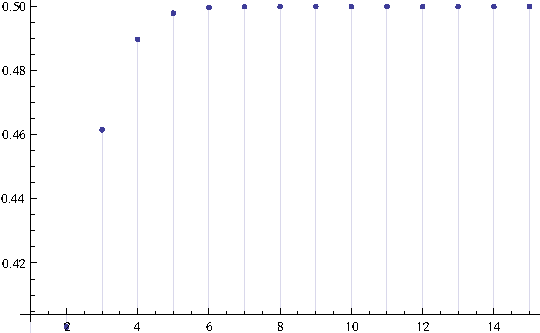
\includegraphics{graphs/nf2nfp1.pdf}
%    \end{center}
%    \label{fig:firstsequence}
%    \caption{A plot of \( a_n = \frac{n!}{2n!+1} \)}
%  \end{figure}
\end{ex}
\begin{defn}\index{converging sequence}
  The sequence \(\{ a_n \}\) \textbf{converges} to the number \(L\) if for every
  positive number \(\varepsilon\) there corresponds an integer \(N\) such that
  for all \(n\)
  \[ n > N \to |a_n - L| < \varepsilon \]
  If \(\{a_n\}\) converges to \(L\), we write \(\lim_{n \to \infty} a_n = L\),
  and call \(L\) the \emph{limit} of the sequence.
\end{defn}
  To really understand this, try thinking of it this way: pick a number $\varepsilon$. It can be very large
  \[ \varepsilon=1000\]
  or really small
  \[ \varepsilon=0.0001\]
  but no matter which one we pick, we can find an index $N$ on the sequence such that for every index past it, we
  are always within $\varepsilon$ of the limit $L$ for the sequence.
  Note that we don't have to know what this number $L$ is, nor what $\varepsilon$ is for that matter, just that
  these numbers exist to state that a sequence is \emph{converging}.
\begin{ex}
  Let us examine the following imaginary sequence:
  \begin{figure}[H]
    \begin{center}
      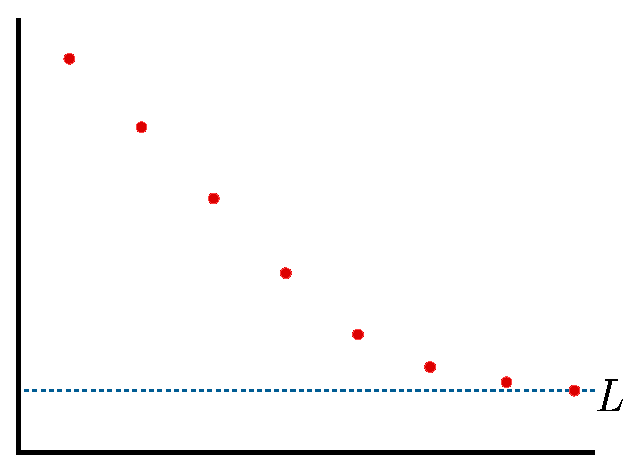
\includegraphics[scale=0.5]{continuous/sequence/conv1}
    \end{center}
    \label{fig:conv1}
  \end{figure}
  Note that for a large $\varepsilon$, our corresponding $N$ occurs very early in the sequence:
  \begin{figure}[H]
    \begin{center}
      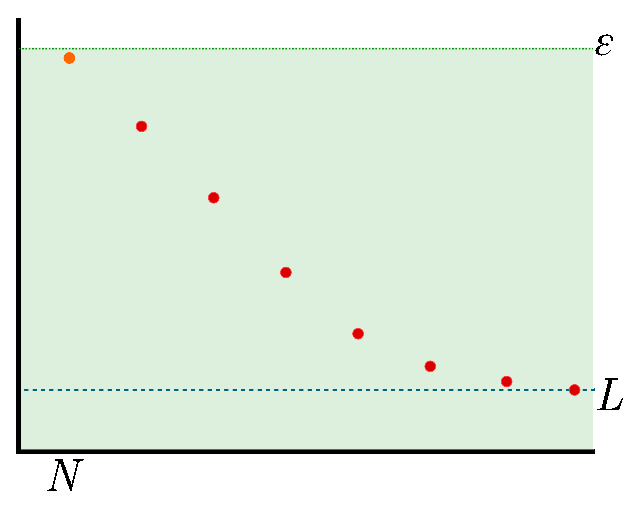
\includegraphics[scale=0.5]{continuous/sequence/conv2}
    \end{center}
    \label{fig:conv2}
  \end{figure}
  However, if we shrink our $\varepsilon$, the number $N$ needed such that every element in the sequence after it
  is within $\varepsilon$ of $L$ gets larger. The real key, however, is that it \emph{always exists}.
  \begin{figure}[H]
    \begin{center}
      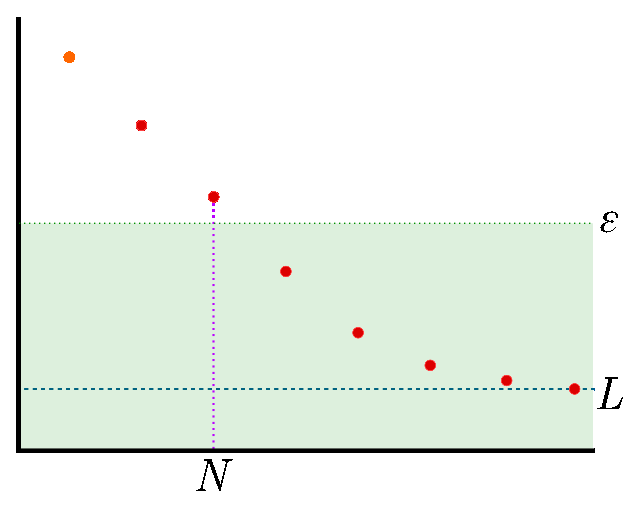
\includegraphics[scale=0.5]{continuous/sequence/conv3}
    \end{center}
    \label{fig:conv3}
  \end{figure}
\end{ex}
\begin{defn}\index{diverging sequence}
  The sequence \(\{ a_n \}\) \textbf{diverges} if the sequence does not converge
  to any number \(L\).

  That is, this number $L$ does not exist.
\end{defn}

\subsection{Bounded Sequences}
\begin{defn}\index{lower bound}
  If there exists a number $m$ such that $m \leq a_n$ for every $n$ we say the sequence is \textbf{bounded below}.
  The number $m$ is called a \textbf{lower bound} for the sequence.
  \begin{figure}[h]
    \begin{center}
      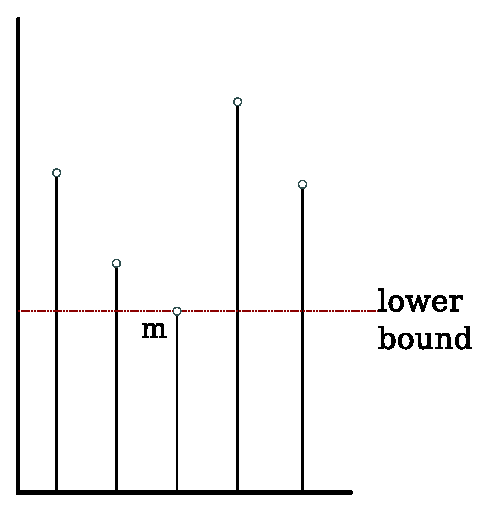
\includegraphics[scale=0.5]{continuous/sequence/lwrbnd}
    \end{center}
  \end{figure}
\end{defn}
\begin{defn}\index{upper bound}
  If there exists a number $M$ such that $a_n \leq M$ for every $n$ we say that the sequence is \textbf{bounded above}.
  The number $M$ is called an \textbf{upper bound} for the sequence.
  \begin{figure}[h]
    \begin{center}
      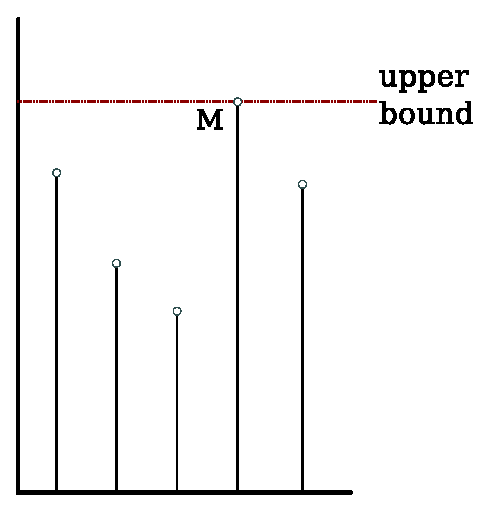
\includegraphics[scale=0.5]{continuous/sequence/uprbnd}
    \end{center}
  \end{figure}
\end{defn}
\begin{defn}\index{bounded}
  If the sequence is both bounded below and bounded above we call the sequence \textbf{bounded}.
\end{defn}
\subsection{Nondecreasing and Nonincreasing Sequences}\label{nondecreasing}
\begin{defn}\index{nondecreasing}
  Given a sequence \(\{a_n\}\), we call the sequence \textbf{nondecreasing} if
  \[\forall n (a_n \geq a_{n-1}).\]
  This means that across the entire sequence, a given element in the sequence is either greater than or equal to the preceeding element.
  A nondecreasing sequence is different from a strictly \emph{increasing} sequence in that it allows for two elements to be equal.
  \begin{figure}[H]
    \begin{center}
      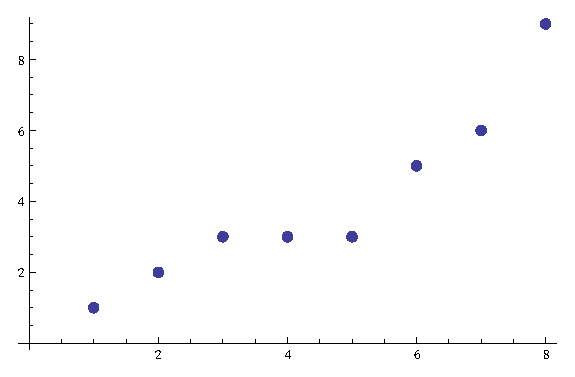
\includegraphics[scale=0.5]{continuous/sequence/nondecreasing}
    \end{center}
    \caption{This sequence is not \emph{increasing} everywhere, although it is \emph{nondecreasing}.}
  \end{figure}
\end{defn}
\begin{defn}
  Given a sequence \(\{a_n\}\), we call the sequence \textbf{nonincreasing} if
  \[\forall n (a_n \leq a_{n-1}).\]
\end{defn}
\begin{defn}
  If \(\{a_n\}\) is either nondecreasing or nonincreasing we call it \textbf{monotonic}.
  \begin{figure}[H]
    \begin{center}
      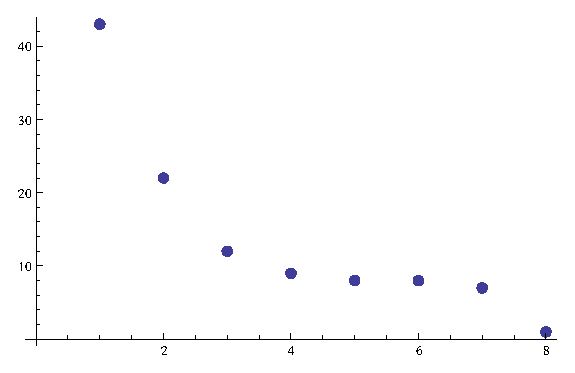
\includegraphics[scale=0.5]{continuous/sequence/nonincreasing}
    \end{center}
    \caption{An example of a nonincreasing sequence.}
  \end{figure}
\end{defn}

\begin{ex}\label{ex:bigsequence}
  \[ a_n=\frac{n+1}{2n-1} \]
    Let's take a more detailed look at an example of a sequence.

    To get a feel for the behavior of the sequence, let's find a few of its
    values:
    \[ \frac{n+2}{2n-1} =
      \left\{3,\frac{4}{3},1,\frac{6}{7},\frac{7}{9},\frac{8}{11}, \cdots \right\} \]


    We could take the derivative of the similar function
    \[ f(x)=\frac{x+2}{2x-1} \]
    to try to figure out what is happening. Since we can assume \(n \geq 1\) for
    our sequence, for \(x \geq 1\) the derivative of \(f(x)\) should also be
    somewhat representative of \(a_n\).
    \begin{align*}
      f'(x)&= \frac{(2 x-1) \left(\frac{\ud}{\ud x}(x+2)\right)-(x+2)
      \left(\frac{\ud}{\ud x}(2 x-1)\right)}{(2 x-1)^2}
      \\
      &=\frac{2 x-2 (x+2)-1}{(2 x-1)^2} \\
      &=-\frac{5}{1-4 x+4 x^2}
    \end{align*}
    \begin{table}[h]
      \centering
      \boxed{
        \begin{tabular}{>\(r<\)|>\(c<\)|>\(c<\)|>\(c<\)}
          x & 0 & 0.5 & 1 \\ \hline
          f'(x) & - & \text{undefined} & -
        \end{tabular}
      }
      \caption{A sign diagram for \(f'(x)\).}
      \label{tab:n51m2xs}
    \end{table}
    \begin{figure}[h]
      \begin{center}
        \includegraphics{graphs/n51m2xs}
      \end{center}
      \caption{A plot of \(f'(x)\).}
      \label{fig:n51m2xs}
    \end{figure}
    Based on Table \ref{tab:n51m2xs}, we can conclude that the sequence is
    nonincreasing. We can therefore describe this sequence as \emph{monotonic}.

    Furthermore, note the end-behavior of this derivative:
    \[ \lim_{x \to \infty} f'(x) = 0 \]
    This implies that, eventually, the rate of change evens off to an indefinitely small number.
    Presumably, this would mean that \(f(x)\) has a horizontal asymptote.
    Based on this information, it seems reasonable to conclude that the sequence \(a_n\) is convering upon a number.
    We do not, however, know to what number it converges.

    To find that, we will need to take the following limit:
    \[ \lim_{n\to\infty} a_n \]
    How do we evaluate limits for sequences? As it turns out, we usually treat
    them exactly the same as limits as functions.
    \begin{theorem}\label{inftyanlimit}\index{limits of sequences}
      Suppose that \(f(x)\) is a function defined for all \( x \geq n_0\) and
      that \( \{a_n\} \) is a sequence of real numbers such that \(a_n = f(n)\)
      for \(n \geq n_0\). Then
      \[ \lim_{x \to \infty} f(x) = L \to \lim_{n \to \infty} a_n = L\text{.} \]
      \begin{proof}
        Suppose that \( \lim_{x \to \infty} f(x) = L \). Then for each positive
        number \( \varepsilon \) there is a number \( M \) such that for all
        \(x\),
        \[ x > M \implies \big| f(x) - L \big| < \varepsilon \]
        Let \(N\) be an integer greater than \(M\) and greater than or equal to
        \(n_0\). Then
        \[ n > N \implies a_n = f(n)\]
        and
        \[\big|a_n -L \big| = \big|f(n) - L\big| < \varepsilon\text{.} \qedhere\]
        \cite[p. 537]{thomas}%Thomas' Calculus, p. 537
      \end{proof}
    \end{theorem}
    This allows us to use \emph{l'Hospital's Rule} to find the limits of some
    sequences. We can state that
    \[\lim_{n\to\infty} a_n =\lim_{n\to\infty}f(x)\]
    assuming
    \[f(x)=\frac{n+1}{2n-1}\text{.}\]
    And thus evaluate the following limit:
    \begin{align*}
      \lim_{n\to\infty} \frac{n+1}{2n-1}
      &\=H \lim_{n\to\infty} \dfrac{\frac{\ud}{\ud x}(n+1)}{\frac{\ud}{\ud x}2n-1} \\
      &\=H \lim_{n\to\infty} \frac{1}{2} \\
      &= \frac{1}{2}
    \end{align*}
    This shows us that the sequence $a_n$ also converges to \(\frac{1}{2}\).
    \begin{figure}[H]
      \begin{center}
        \includegraphics{graphs/np22nm1.pdf}
      \end{center}
      \caption{A graph of the sequence $ a_n=\frac{n+1}{2n-1} $.}
    \end{figure}
\end{ex}
\begin{ex}
  Demonstrate that $\{n!\}$ is nondecreasing.
  \begin{sol}
    First let us look at the definition for a factorial.
    \begin{equation}\label{eq:factorial}\index{factorial}
      n! =
      \begin{cases}
        1 & \text{if } n = 0, \\
        n(n-1)! & \text{if } n > 0
      \end{cases}
    \end{equation}
    \begin{proof}
      Remember our definition for a nondecreasing sequence from \ref{nondecreasing}:
      \[\forall n (a_n \geq a_{n-1})\text{.}\]
      Let us assume that this holds true for our sequence $\{n!\}$ when $n>1$.
      \begin{align*}
        n!&\geq(n-1)!& n&>1 \\
        \intertext{Divide each side by $(n-1)!$}
        \frac{n!}{(n-1)!}&\geq \frac{(n-1)!}{(n-1)!} &n&>1 \\
        \frac{n!}{(n-1)!}&\geq 1 &n&>1 \\
        \intertext{Now, remembering our definition for the factorial,}
        \frac{n(n-1)!}{(n-1)!}&\geq 1 &n&>1 \\
        n&\geq1 &n&>1\qedhere
      \end{align*}
    \end{proof}
    % \begin{proof}
    %   \begin{align*}
    %     \underbrace{n!}_{n(n-1)} > (n-1)!
    %     n(n-1)! &> (n-1)! \\
    %     n(n-1)! - (n-1)! &> 0 \\
    %     (n-1)! [n-1] &> 0 \qedhere
    %   \end{align*}
    % \end{proof}
  \end{sol}
\end{ex}
\begin{ex}
  Show that the sequence \[ \{a_n\} = \left\{ \frac{n+2}{2n-1} \right\}^{\infty}_{n=1} \] is nonincreasing.
  \begin{sol}
    This example is very similar to Example \ref{ex:bigsequence}, with only a
    change of constant in the numerator. We will demonstrate this sequence's
    behavior using a different method than before, however.

    Another way we can demonstrate that a sequence is decreasing is by using
    the definition of a \emph{decreasing sequence}: \(\forall n ( a_n <
    a_{n-1})\). We simply substitute in \(n\) and \(n-1\) on the
    respective sides of the inequality.
    \begin{proof}
      \begin{align*}
        \forall n (a_n &< a_{n-1}) &n&>1 \\
        \frac{n+2}{2n-1} &< \frac{(n-1)+2}{2(n-1)-1} &n&>1 \\
        \frac{n+2}{2n-1} &< \frac{n+1}{2n-3} &n&>1 \\
        \left(\frac{2n-3}{2n-3}\right) \left( \frac{n+2}{2n-1} \right)
        &< \left(\frac{n+1}{2n-3}\right) \left(\frac{2n-1}{2n-1}\right)
        &n&>1\\
        \frac{2n^2-3n+4n-6}{4n^2-6n-2n+3} &< \frac{2n^2+2n-n-1}{4n^2-6n-2n-3} &n&>1\\
        \frac{2n^2+n-6}{4n^2-8n+3}&<\frac{2n^2+n-1}{4n^2-8n-4} &n&>1 \\
        2n^2+n-6 &< 2n^2+n-1 &n&>1 \\
        -6 &< -1 &n&>1 \qedhere
      \end{align*}
    \end{proof}
  \end{sol}
\end{ex}
% \begin{ex}
%   Is
%   \[ \left\{\frac{n}{n+1} \right\} \]
%   monotonic?
%   \begin{sol}
%       \begin{align*}
%         \lim_{n\to\infty} \frac{n}{n+1}=1
%       \end{align*}
%       \begin{align*}
%         f(x)&=\frac{x}{x+1} \\
%         f'(x)&=\frac{(x+1)1-x(1)}{(x+1)^2} \\
%         f'(x)&=\frac{1}{(x+1)^2}
%       \end{align*}
%   \end{sol}
% \end{ex}
\begin{ex}
  Show that
  \[ \left\{ \frac{n}{n+1} \right\} \]
  is monotonic increasing.
  \begin{sol}
    \begin{proof}
      \[ \forall n > 1 \left(  a_n > a_{n-1}  \right) \]
      \begin{align*}
        a_n &> a_{n-1}\\
        \frac{n}{n+1} &> \frac{n-1}{n-1+1} \\
        \frac{n}{n} \frac{n}{n+1} &> \frac{n-1}{n}\frac{n+1}{n+1} \\
        n^2 &> (n-1)(n+1)\\
        n^2 &> n^2-1 \\
        0 &> -1 \qedhere
      \end{align*}
    \end{proof}
  \end{sol}
\end{ex}
\begin{ex}
  Does
  \[ a_n = \frac{n+1}{2^n} \]
  converge or diverge?
  \begin{sol}
    Remembering that we can rewrite \(2^n\) as
          \( e^{n \cdot \ln{2}} \)
    \begin{align*}
      \lim_{n \to \infty} \frac{n+1}{2^n}
      &= \lim_{n \to \infty} \frac{n+1}{e^{n\cdot \ln{2}}} \\
      &\=H \lim_{n \to \infty} \frac{1}{\ln2 \cdot e^{n\ln2}}\\
      &= \lim_{n \to \infty} \frac{1}{\ln2 \cdot 2^n}
      \intertext{Using the constant multiple rule for limits of sequences, we
      can pull out the \( \ln 2 \). }
      &= \frac{1}{\ln 2}\cdot \left(\lim_{n \to \infty}
      \frac{1}{2^n}\right)
    \end{align*}
    \(\{\frac{1}{2^n}\}\) is converging very quickly toward 0,
    so \(a_n\) as well must converge to \(0\).
    \begin{figure}[h]
      \begin{center}
        \includegraphics{graphs/oneovertwoton}
      \end{center}
      \caption{A plot of \(\{\frac{1}{2^n}\}\).}
      \label{fig:oneovertwoton}
    \end{figure}
  \end{sol}
\end{ex}
\begin{ex}
  Does
  \[ \left\{ \frac{1}{n!} \right\} \]
  converge or diverge?
  \begin{sol}
      \begin{align*}
        \lim_{n \to \infty} \frac{1}{n!} = 0
      \end{align*}
  \end{sol}
  Alternatively, we could demonstrate that the sequence is bounded and monotonic.
\end{ex}
\begin{ex}
  Does
  \[ a_n = \frac{2^n}{n!} \]
  converge or diverge?
  \begin{sol}
    We can show this, intuitively, as follows:
    \begin{align*}
      a_n = \left\{
        \frac{2\times2\times2\times2\times2\times\ldots}{1+2+3+4+5+6+\ldots} \right\}
    \end{align*}
    But the actual proof requires the \emph{sandwich theorem for
    sequences}\cite[p.~536]{thomas}:
    \begin{theorem}[The Sandwich Theorem for Sequences]\index{The Sandwich
      Theorem for Sequences}\label{th:sandwichsequence}
      Let $\{a_n\}$, $\{b_n\}$, and $\{c_n\}$ be sequences of real numbers. If
      $a_n \leq b_n \leq c_n $ holds for all $n$ beyond some index $N$, and if
      $\lim_{n\to\infty} a_n = \lim_{n\to\infty} c_n = L$, then
      $\lim_{n\to\infty} b_n = L$ also.
    \end{theorem}
      A proof of this theorem is found in \ref{proof:sandwichsequence}.
      By Theorem \ref{th:sandwichsequence}, \[\lim_{n \to \infty} a_n =
      \lim_{n\to\infty}\frac{2^n}{n!}=0.\]
  \end{sol}
\end{ex}
\begin{ex}
  \[ a_n = \frac{(-1)^n}{n!} \]
  \begin{sol}
    Consider
    \begin{align*}
      b_n = \left| \frac{(-1)^n}{n!} \right| = \frac{1}{n!} = 0
    \end{align*}
    Intuitively, we can also state that $a_n$ should converge.
    Using Theorem \ref{th:sandwichsequence}, we can determine that this sequence converges.
    % Review \emph{bounded and monotonic} for sequences, txtbg pg 536.
    % That's in Thomas' calculus. -[Nathan]
  \end{sol}
\end{ex}
\begin{ex}
  \[ a_n = \frac{1}{n-0.\bar{9}} \]
  \begin{sol}
    A sequence can be unbounded, and still converge.

    $0.\bar{9}$ is very close to $1$, close enough that we can treat it as $1$ as $n\to\infty$.
    Doing so, it becomes clear that this sequence converges, as $\frac{1}{n-1}$ converges.
    Consider, however, the very first term, where $n=1$.
    This term is \emph{gigantic}, essentially \(\infty\).
    The sequence is not bounded, yet it still manages to converge.
    This sequence converges to \(0\).
  \end{sol}
\end{ex}
\begin{ex}
  Does the following sequence converge?
  \[ a_n = \left( \frac{n+8}{9n} \right) \left( 1-\frac{8}{n} \right) \]
  Find the limit if the sequence is convergent.
  \begin{sol}
    Remembering that a limit of products is a product of limits,
    \begin{align*}
      \lim_{n \to \infty} \left( \frac{n+8}{9n} \right) \left( 1-\frac{8}{n} \right)
      &= \lim_{n \to \infty} \left( \frac{n+8}{9n} \right) \cdot
      \lim_{n \to \infty} \left( 1-\frac{8}{n} \right)\\
      &= \frac{1}{9}
    \end{align*}
    The sequence converges to \(\frac{1}{9} \).
  \end{sol}
\end{ex}
\begin{ex}
  Show that the sequence \[a_n = \frac{2}{n^2} \] is monotonic and bounded.
  \begin{sol}
    Treat the sequence as a function $f(x)$ and take the derivative.
    \[ f(x) = \frac{2}{x^2} \]
    \[ f'(x) = -4 x^{-3} \]
    $f'(x)$ is negative on the interval $[1, \infty)$, so $f(x)$ is decreasing
      on the interval $[1, \infty)$. Since the sequence goes from $1$ to
        $\infty$ and is always decreasing, its upper bound must be at $n=1$.
        $a_1=2$, the upper bound for the sequence. To find the lower bound, we
        take the limit as $n \to \infty$:
        \[ \lim_{n \to \infty} a_n = \lim_{n \to \infty} \frac{2}{n^2} = 0 \]
        Which shows us that $0$ is the lower bound of the sequence.

        Thus, we can conclude that the sequence is monotonic and bounded, and therefore converges.
  \end{sol}
\end{ex}
\begin{ex}
  Find a formula for the nth term of the sequence where \(a_n\) is calculated
  directly from \(n\).
  \[ \frac{1}{1}, \frac{4}{2}, \frac{7}{6}, \frac{10}{24}, \frac{13}{120} \cdots \]
  \begin{sol}
    We basically have to just take close guesses and see if we can make a sequence that follows this.

    Doing so, we will find that the answer is
    \[ a_n = \frac{3n-2}{n!}.\]
  \end{sol}
\end{ex}

% \begin{homework}
%     Wolfram Mathematica assingment and MyMathLab homework due Friday, March 23, 2012.
% \end{homework}
% \begin{homework}
%   Read Section 10.2
%
%   pg. 551 ALL 27-34, 35, 36, 37, 38, 41, 43, 49, 50, 51, 55, 56, 57, 58, 59, 61
% \end{homework}
%

\chapter{Infinite Series}
\label{ch:series}

An infinite series is the sum of an infinite sequence of numbers
\[ a_1 + a_2 + a_3 + \cdots + a_n + \cdots \]
Given a sequence $\{a_n\}$, the number $a_n$ is the \textbf{$n$th term} of the
series. The sequence $\{s_n\}$ is the \textbf{sequence of partial sums} of the
series, defined by
\begin{align*}
  s_1 &= a_1 \\
  s_2 &= a_1 + a_2 \\
  & \vdots \\
  s_n &= a_1 + a_2 + \cdots + a_n = \sum^\infty_{k=1} a_k \\
  & \vdots
\end{align*}
The number $s_n$ represents the \textbf{$n$th partial sum} of the infinite
series.

The partial sum \(s_n\) of a series can also be given by
  \[ s_n = s_{n-1} + a_n .\]

If the sequence of partial sums converges to a limit $L$, we say that
the series \textbf{converges} and that its \textbf{sum} is $L$. In this case, we
also write
\[ a_1 + a_2 + a_3 + \cdots + a_n + \cdots = \sum_{n=1}^\infty a_n = L \]
If the sequence of partial sums of the series does not converge, then we say
that the series \textbf{diverges}.
\cite[p.~544]{thomas}

Given a series, we will usually want to know whether it converges or diverges,
and if it converges, then to what number?

For converging series, there are some rules that can aid us:
\begin{theorem}\label{th:combiningseries}
  If $\sum a_n = A$ and $\sum b_n = B$ are convergent series, then
  \begin{table}[H]
    \centering
    \begin{tabular}{ll>$r<$}
    1. & Sum Rule & \sum (a_n+b_n) = \sum a_n + \sum b_n = A +B \\
    2. & Difference Rule & \sum (a_n-b_n) = \sum a_n - \sum b_n = A -B \\
    3.& Constant Multiple Rule & \sum ka_n = k\sum a_n = kA \text{ for any
    $k$}
    \end{tabular}
  \end{table}
\end{theorem}

% \begin{remark}
%   When discussing a series,
%   \[
%     \sum{i=1}^\infty f(x) \text{ is better written }\sum{i=1}^\infty a_n
%     \text{.}
%   \]
% \end{remark}

\section{Limit Test}\index{series limit test}

When presented with a series, such as
\[ \sum^\infty_{n=1} \frac{n!}{2n!+1}, \]
if we wish to know whether it converges or diverges, we should generally first
confirm that the series does not diverge before trying to determine its
convergence.

For a series like this, it is better to think of it as a sum of numbers in a
sequence, $\{a_n\}$, than as a sum operator operating on a function. In this
case, $\{a_n\}$ would equal
\[ \frac{n!}{2n!+1} \]

Now think about it--if this $\{a_n\}$ is converging to any number other than
$0$, then as our $n$ goes toward $\infty$, we will always have numbers to add.
The sequence will continue growing. That is, the sequence will diverge.

So we should take the following limit:
\[ \lim_{n \to \infty} \frac{n!}{2n!+1} \]
How do we calculate the limit of a sequence involving $n!$? Our limit rules tell
us nothing about evaluating factorials. We can, however, use a creative little trick
common in evaluating limits of polynomials: divide each term in both the
numerator and denominator by the term of the highest power.
\begin{align*}
  \lim_{n \to \infty} \frac{n!}{2n!+1} &=
  \frac{\frac{n!}{n!}}{\frac{2 \cdot n!}{n!}+\frac{1}{n!}} \\
  &= \frac{1}{2 + \frac{1}{n!}} \\
  \intertext{Now, think about where the term $\frac{1}{n!}$ is heading as $n
  \to \infty$. The denominator is getting huge, and very quickly, as if there
  were a high degree power of $x$ in the denominator of a limit. In that case,
  $1/x^k$ would become meaningless--it would essentially disappear, so $1/n!$
  must also go to $0$.}
  &= \frac{1}{2+0} \\
  \lim_{n \to \infty} a_n &=\frac{1}{2}
\end{align*}
So the limit of $\{a_n\}$ as $n$ approached $\infty$ is not zero. Thus, the
\emph{$n$th term} of the series, no matter how large $n$ becomes, will never be
zero. The series is always adding more numbers, and that means it is
\textbf{diverging}.

It is worth noting that if, indeed, the \(\lim_{n\to \infty}\) of \( \{a_n\} \) did equal $0$, this would
tell us nothing about the convergence or divergence of the series.

\begin{theorem}\label{th:nthtermdiv}
  The series $\sum^\infty_{n=1} a_n$ diverges if \(\lim_{n\to \infty} a_n \neq 0
  \).
  \begin{proof}
    We prove this by contrapositive, described in Section
    \ref{app:def:contrapositive}. The statement we are trying to prove is:
    \begin{quote}
      If \(\lim_{n\to \infty} a_n \neq 0 \) then the series diverges.
    \end{quote}
    We could write this as $P \to Q$ where $P$ represents ``The limit of $a_n$
    as $n \to \infty$ is nonzero'' and $Q$ represents ``the series diverges.''
    Thus, the contrapositive of this proposition would be $\neg Q \to \neg P$.
    If we can prove the contrapositive, then the original statement must be
    true.
    We would $\neg Q \to \neg P$ as:
    \begin{quote}
      ``If a series is convergent, then \( \lim_{n \to \infty} a_n = 0\).''
    \end{quote}
    Now, let $L$ represent the series' sum.
    \begin{align*}
      s_n &= s_{n-1} + a_n \\
      \lim_{n \to \infty} s_n &= \lim_{n \to \infty} s_{n-1} + a_n \\
      L&=L + \lim_{n\to \infty} a_n \\
      \lim_{n\to \infty} a_n &= 0\qedhere
    \end{align*}
  \end{proof}
\end{theorem}

\begin{ex}
  Does the series
  \[ \sum^\infty_{n=1} \frac{6n}{6n+1} \]
  diverge or converge?
  \begin{sol}
    Take \( \lim_{n\to\infty} \frac{6n}{6n+1} \).
    \begin{align*}
      \lim_{n\to\infty} \frac{6n}{6n+1}
      &\=H \lim_{n\to\infty} \frac{6}{6} \neq 0
    \end{align*}
    By Theorem \ref{th:nthtermdiv}, the series diverges.
  \end{sol}
\end{ex}

\section{Harmonic Series}

\begin{ex}
  The series
  \[ \sum_{n=1}^{\infty} \frac{1}{n} \]
  is called the \textbf{harmonic series}. How does this series behave?
  \begin{remark}
    Just because
    \[ \lim_{n \to \infty} \frac{1}{n}\]
    is zero does not imply anything about convergence or divergence.
  \end{remark}

  We can try finding some of its partial sums:
  \begin{align*}
    s_1 & = 1 \\
    s_2 & = 1 + \frac{1}{2} \\
    s_3 & = 1 + \frac{1}{2} + \frac{1}{3} \\
    s_4 & = 1 + \frac{1}{2} + \frac{1}{3} + \frac{1}{4} \\
    &\vdots \\
    s_n & = 1 + \frac{1}{2} + \frac{1}{3} + \frac{1}{4} + \cdots + a_n
  \end{align*}
  Notice that as we continue to add terms, we could group them in the following
  way:
  \begin{align*}
    s_n &= 1 + \frac{1}{2} + \bigg( \frac{1}{3} + \frac{1}{4} \bigg)
    + \bigg( \frac{1}{5} + \frac{1}{6} + \frac{1}{7} + \frac{1}{8} \bigg)
    + \bigg( \frac{1}{9} + \frac{1}{10} + \cdots + \frac{1}{16} \bigg)
    + \cdots\\
    &= 1 + \frac{1}{2} + \bigg( \frac{7}{12} \bigg)
    + \bigg( \frac{533}{840} \bigg)
    + \bigg( \frac{95549}{144144} \bigg)
    + \cdots \\
    &\approx 1+ 0.5 + (0.583333) + (0.635424) + (0.662872) + \cdots
  \end{align*}
  The series is increasing indefinitely, just doing it very slowly.
  \end{ex}


\section{Geometric Series}\index{geometric series}

\textbf{Geometric Series} are series of the form
\[a + ar + ar^2 +\cdots +ar^{n-1}+\cdots=\sum_{n=1}^\infty ar^{n-1} \]
in which $a$ and $r$ are fixed real numbers and $a \neq 0$. The series can also
be written as $\sum_{n=0}^\infty ar^n$, where the only difference is the
starting value of $n$. The ratio $r$ can be positive or negative.

If $r=1$, the $n$th partial sum of the geometric series is
\[ s_n=a+a(1)+a(1)^2+\cdots+a(1)^{n-1}=na \]
and the series diverges because $\lim_{n \to\infty} s_n = \pm \infty$.

If $r=-1$, the series diverges because the $n$th partial sums alternate between
$a$ and $0$.

If $|r| \neq 1$, we can determine the convergence or divergence of the series in
the following way:

\begin{align*}
  s_n &= a + ar + ar^2 + \cdots + ar^{n-1} \\
  rs_n &= ar + ar^2 + ar^3 + \cdots + ar^{n-1} + ar^n \\ \intertext{Multiply $s_n$ by
  $r$.}
  s_n - rs_n &= \left[ a + ar + ar^2 + \cdots + ar^{n-1} \right]
  -\left[ ar + ar^2 + ar^3 + \cdots + ar^{n-1} + ar^n \right] \\
  \intertext{Subtract $rs_n$ from $s_n$.}
  s_n-rs_n &= \left( a \right)+\left( ar - ar \right)+ \left( ar^2 -
    ar^2   \right) + \cdots + \left( ar^{n-1}-ar^{n-1} \right)-ar^n \\
  \intertext{Rearrange and the inner terms cancel.}
  s_n - rs_n &= a - ar^n \\
  s_n(1-r) &= a(1-r^n) \\ \intertext{Factor.}
  s_n &= \frac{a(1-r^n)}{1-r}, \quad (r \neq 1).
\end{align*}
If $|r| < 1$, then $r^n \to 0$ as $n \to 0$ and $s_n \to a/(1-r)$. If $|r| > 1$,
then $|r^n| \to \infty$ and the series diverges.\cite[p.~546]{thomas}

\begin{ex}
  \[ \sum_{n=1}^{\infty} \frac{3^n+2^n}{6^n} \]
  \begin{sol}
    This is a sum of two series. Theorem \ref{th:combiningseries} tells us that
    a series of a sum of converging series is a sum of series.

    Thus,
    \[ \sum_{n=1}^{\infty} \frac{3^n+2^n}{6^n}=\sum_{n=1}^\infty
      \frac{3^n}{6^n} + \sum_{n=1}^\infty \frac{2^n}{6^n}, \]
    assuming both of these series converge.

    Let us look at the first series:
    \[ \sum_{n=1}^\infty \frac{3^n}{6^n} \]
    If we write out some of the terms:
    \begin{align*}
      s_n
      &=\frac{1}{2}+\frac{1}{4}+\frac{1}{8}+\frac{1}{16}+\frac{1}{32} + \cdots
      \\
      s_n &=0+\left( \frac{1}{2} \right) + \left( \frac{1}{2} \right)^2 + \left(
      \frac{1}{2} \right)^3 + \cdots + \left( \frac{1}{2} \right)^{n-1} \\
      \intertext{we can see that we are handling a geometric series with $a=0$
      and $r=1/2$. Thus,}
      \frac{1}{2}\cdot s_n &= \left( \frac{1}{2} \right)^2 + \left( \frac{1}{2} \right)^3 + \left(
      \frac{1}{2} \right)^4 + \cdots + \left( \frac{1}{2} \right)^{n-1} + \left(
      \frac{1}{2} \right)^n \\
      s_n - \frac{1}{2} \cdot s_n &=\left( \frac{1}{2} \right)+{\bigg(
        \left( \frac{1}{2} \right)^2 - \left( \frac{1}{2} \right)^2 \bigg) +
        \bigg( \left( \frac{1}{2} \right)^3 - \left( \frac{1}{2} \right)^3
        \bigg) + \cdots + \bigg( \left( \frac{1}{2} \right)^{n-1} -\left(
        \frac{1}{2} \right)^{n-1} \bigg)} - \left( \frac{1}{2} \right)^n \\
        \intertext{The inner terms cancel:}
        s_n - \frac{1}{2} \cdot s_n &= \frac{1}{2}-\left( \frac{1}{2} \right)^n
        \\
        s_n \left( 1 - \frac{1}{2} \right) &= \frac{1}{2} -\left(
        \frac{1}{2}\right)^n \\
        s_n &=\frac{1/2-\left(1/2\right)^n}{1 - 1/2} \\
      \end{align*}
        Now we take the limit of both sides of the equation.
      \begin{align*}
        \lim_{n\to\infty} s_n &=\lim_{n\to\infty}\frac{1/2 - 0}{1 - 1/2} \\
        \intertext{
          As $n \to \infty$, $(1/2)^n \to 0$.
        }
        &=\lim_{n\to\infty}\frac{1}{2(1-1/2)}
        =\lim_{n\to\infty} \frac{1}{2-1}
        =\lim_{n\to\infty} \frac{1}{1} \\
        &=1
    \end{align*}
    From this, we realize that that
    \( \sum_{n=1}^\infty \frac{3^n}{6^n} \)
    converges to 1.

    The second series is quite similar:
    \[ \sum_{n=1}^\infty \frac{2^n}{6^n} \]
    Also a geometric series, we will find that
    \begin{align*}
      s_n &= \frac{1}{3}+\frac{1}{9}+\frac{1}{27}+\frac{1}{81}+ \cdots + \left(
      \frac{1}{3} \right)^{n-1} \\
      s_n\left( 1-1/3 \right)&=\left( 1/3-(1/3)^n \right) \\
      s_n &= \frac{1/3-(1-3)^n}{1-1/3} \\
    \end{align*}
    Taking the limit as $n \to \infty$ of both sides:
    \begin{align*}
      \lim_{s_n\to\infty} s_n &= \lim_{s_n\to\infty} \frac{1/3-(1-3)^n}{1-1/3} \\
      &= \lim_{s_n\to\infty} \frac{1}{3(1-1/3)} \\
      &= \frac{1}{2}
    \end{align*}
    \begin{figure}[h]
      \begin{center}
        \subfigure[A plot of \( \sum_{n=1}^\infty
          \frac{3^n}{6^n}\).]{
          \includegraphics[scale=0.8]{continuous/series/series-3n6n.eps}
        }
        \subfigure[A plot of \( \sum_{n=1}^\infty \frac{2^n}{6^n}. \)]{
          \includegraphics[scale=0.8]{graphs/2pn6pn.eps}
        }
        \subfigure[A plot of \( \sum_{n=1}^\infty \frac{3^n+2^n}{6^n}\).]{
          \includegraphics[scale=0.8]{graphs/3pn2pn6pn.eps}
        }
      \end{center}
    \end{figure}

    Finally,
    \begin{align*}
      \sum_{n=1}^{\infty} \frac{3^n+2^n}{6^n}&=\sum_{n=1}^\infty
      \frac{3^n}{6^n} + \sum_{n=1}^\infty
      \frac{2^n}{6^n} \\
      &=1+\frac{1}{2} \\
      &= \frac{3}{2}
    \end{align*}
    \end{sol}
\end{ex}

\section{The Comparison Test}\index{series comparison test}

\begin{theorem}[The Comparison Test]\label{th:seriescomp}
  Let $\sum a_n$, $\sum c_n$, and $\sum d_n$ be series with nonnegative terms.
  Suppose that for some integer $N$
  \[ \forall n > N \bigg(d_n \leq a_n \leq c_n\bigg) \]

  \textbf{(a)} If $\sum c_n$ converges, then $\sum a_n$ also converges.

  \textbf{(b)} If $\sum d_n$ diverges, then $\sum a_n$ also diverges.
\end{theorem}

\section{The Integral Test}\index{series integral test}

Another helpful tool for discovering the behavior of a series is the
\emph{integral test}. In simple terms it is present as follows:
Given the following two statements:
\begin{enumerate}
  \item \(f' < 0 \text{ over } [\ldots, \infty) \)
  \item \(f(n)\) is always positive. We can often see this by writing out some terms.
\end{enumerate}
The integral test states that:

\begin{align*}
  \text{\textbf{(a)}} & \sum^\infty_{n=\ldots} f(n) \text{ converges if }
  \int_{\ldots}^{\infty} f(x) \ud x \text{ converges.}  \\
  \text{\textbf{(b)}} & \sum^\infty_{n=\ldots} f(n) \text{ diverges if } \int_{\ldots}^{\infty} f(x) \ud x \text{ diverges.}
\end{align*}

\begin{proof}
  \begin{align*}
    \int^\infty_1 f(x) \ud x
    &\approx f(1) \Delta x + f(2) \Delta x + f(3) \Delta x + \cdots + \text{with } \Delta x = 1 \\
    &\approx f(1) + f(2)+f(3)+\cdots \\
    &\approx \sum^\infty_{n=1} f(n)\qedhere
  \end{align*}
\end{proof}

\begin{theorem}[The Integral Test]\label{th:seriesint}
  Let $\{a_n\}$ be a sequence of positive terms. Suppose that $a_n = f(n)$,
  where $f$ is a continuous, positive, decreasing function of $x$ for all $x
  \geq N$ ($N \in \mathbb{Z_+}$). Then the series $\sum_{n=N}^\infty a_n$ and
  the integral $\int_N^\infty f(x)\ud x$ both converge or both
  diverge.\cite[p.~554]{thomas}
\end{theorem}

\begin{ex}\label{famousp}
  How do we know that the following series
  \[ \sum^\infty_{n=1} \frac{1}{n} \]
  diverges?
  \begin{sol}
    First, we test it with Theorem \ref{th:nthtermdiv}.
    \[ \lim_{n\to\infty} \frac{1}{n}=0\]
    Because this limit is zero, the test proves inconclusive.

    Let's check the two prerequisites for the integral test. If we let
    $\sum^\infty_{n=1} \frac{1}{n}$ be $\sum^\infty_{n=1}$, and $a_n =
    \frac{1}{n}$, then we can treat $a_n$ as a function and make sure it is
    positive and always decreasing.

    The function \[ f(x)=\frac{1}{x} \]is always positive on $[1, \infty)$.
    Its derivative, \[f'(x)=-\frac{1}{x^2}\] is always negative. Thus, we can
    use the integral test to describe the behavior of $\sum^\infty_{n=1} a_n$.
    \[
      \int^\infty_1 \frac{1}{n} = \lim_{t\to\infty} \ln x |^\infty_1
    \]
    This integral diverges, so by Theorem \ref{th:seriesint} the series also
    diverges.
%%    Note that it it is better to think:
%%    \[ \sum a_n \to \sum^\infty_{n=\ldots} f(n) \]
%%
%%    \[ \sum^\infty_{n=1} \frac{1}{n} \to \int^\infty_1 \frac{1}{x}\ud x \]
%%    \begin{align*}
%%      \int^\infty_1 \frac{1}{x}\ud x
%%      \text{ is }
%%      \int^t_1 \frac{1}{x} \ud x
%%    \end{align*}
  \end{sol}
\end{ex}
\begin{ex}
  Determine whether the following series is convergent or divergent.
  \[ \sum_{k=4}^\infty k e^{-k^2} \]
  \begin{sol}
    We can use the integral test.
    \begin{align*}
      \int_{k=4}^\infty k e^{-k^2} \ud k
      &=\frac{-1}{2}\int_{k=4}^\infty -2 k e^{-k^2} \ud k \\
      &=\frac{-1}{2}e^{-x^2} \bigg|_4^\infty
    \end{align*}
    We can tell that this integral converges, so the series converges.
  \end{sol}
\end{ex}


\section{p Series}

A \(p\) series is of the form.

\[ \sum_{n=1}^{\infty} \frac{1}{n^p} \]

At \(p=1\), it diverges because of the integral test.
This is actually a famous instance of the \(p\)-series.

At \(p=2\), the series converges.

At \(p=-1\), the series diverges.

At \(p=-2\), the series diverges by \ref{th:nthtermdiv}.

At \(p=1.0000000000001\), the series converges by the integral test.

We can get a feeling that \( p>1 \) leads to convergence, and \(p <= 1\) leads to a diverging series.

\begin{homework}
  Online assignment due 04 April 2012 at midnight.

  The next one is due Friday 07 April 2012 at midnight.
\end{homework}

\section{Encyclopedia of Series}

\subsection{Converging series}
\begin{ex}\label{ex:convcomp}
  \[ \sum_{n=1}^{\infty} \frac{5+2\sqrt n}{n^3} \]
  \begin{sol}

    Let $f(x)=\frac{5+2\sqrt{x}}{x^3}$, which is always positive on $x\geq 1$.
    Then $f'(x) = -\frac{5(\sqrt{x}+3)}{x^4}$, which is always negative on $x
    \geq 1$.
    \begin{figure}[h]
      \begin{center}
        \subfigure[A plot of $f(x)=\frac{5+2\sqrt{x}}{x^3}$.]{
          \includegraphics[scale=0.8]{graphs/5p2sqxx3.eps}
        }
        \subfigure[A plot of $f(x)=\frac{5+2\sqrt{x}}{x^3}$.]{
          \includegraphics[scale=0.8]{graphs/n5xp3x4.eps}
        }
      \end{center}
    \end{figure}
    \begin{align*}
      \int_1^\infty \frac{5+2\sqrt x}{x^3} \ud x
      &= \int_1^\infty \frac{5}{x^3} \ud x
      + \int_1^\infty \frac{2 \sqrt x}{x^3} \ud x \\
      &= \int_1^\infty 5x^{-3} \ud x
      + \int_1^\infty 2x^{1/2} \cdot x^{-3} \ud x \\
      &= \lim_{t\to\infty} \int_1^t 5x^{-3} \ud x
      +  \lim_{t\to\infty}\int_1^t 2x^{-5/2} \ud x \\
      &= \lim_{t\to\infty}\frac{5x^{-2}}{-2}\bigg|_1^t+
      \lim_{t\to\infty}\frac{2x^{-3/2}}{-3/2}\bigg|_1^t \\
      &= \lim_{t\to\infty} \bigg[-\frac{5t^{2}}{2}+\frac{4(1)^{-3/2}}{3} \bigg]
      + \lim_{t\to\infty}\bigg[ -\frac{4t^{-5/2}}{3} +\frac{4(1)^{-3/2}}{3}
        \bigg] \\
      &=\lim_{t\to\infty} \bigg[-\frac{5t^{-2}}{2}+\frac{5}{2} \bigg]
      + \lim_{t\to\infty}\bigg[ -\frac{4t^{-3/2}}{3} +\frac{4}{3}
        \bigg]\\
      &=\lim_{t\to\infty} -\frac{5t^{-2}}{2}+\lim_{t\to\infty} \frac{5}{2}
      + \lim_{t\to\infty} -\frac{4t^{-3/2}}{3} +\lim_{t\to\infty}\frac{4}{3} \\
      &=\frac{23}{6}-\lim_{t\to\infty}\bigg[
        \frac{5t^{-2}}{2}+\frac{4t^{-5/2}}{5} \bigg] \\
      &=\frac{23}{6}-\lim_{t\to\infty}\bigg[
        \frac{5}{2t^2}+\frac{4}{3t^{3/2}} \bigg]\\
        &=\frac{23}{6}+0 \\
        &= \frac{23}{6}
    \end{align*}
    By Theorem \ref{th:seriesint}, the series
    \( \sum_{n=1}^{\infty} \frac{5+2\sqrt n}{n^3} \)
    converges.
  \end{sol}
\end{ex}
\begin{ex}
  \[ \sum_{n=1}^{\infty} \frac{5+2\sqrt{n}}{n^3+1} \]
  We can tell that this is quite similar to Example \ref{ex:convcomp}, except we are making the denominator larger.
  We can tell by comparison with the original problem that this must also converge. Likewise, if we made the numerator smaller, we could treat this as converging.
  For a proper solution, we would write
  \begin{sol}
    \[ \sum_{n=1}^{\infty} \frac{5+2\sqrt{n}}{n^3+1} \]
    Converges by comparison with \( \sum_{n=1}^{\infty} \frac{5+2\sqrt n}{n^3} \).
  \end{sol}
  \begin{figure}[h]
    \begin{center}
      \subfigure[A plot of $s_n=\frac{5+2\sqrt{n}}{n^3}$]{
        \includegraphics[scale=0.8]{graphs/5p2sqn3.eps}
      }
      \subfigure[A plot of $s_n=\frac{5+2\sqrt{n}}{n^3+1}$]{
        \includegraphics[scale=0.8]{graphs/5p2sqn3p1.eps}
      }
    \end{center}
  \end{figure}

  Make note, however, that making the denominator smaller does not help us in making these comparisons for convergence.
\end{ex}
\begin{ex}
  \[ \sum_{n=1}^{\infty} \frac{1}{n^4} \]
  This converges.

  \[ \sum_{n=1}^{\infty} \frac{1}{n^4+2} \]
\end{ex}
\begin{ex}
  \[ \sum_{n=1}^{\infty} \frac{2}{n^2+4n+3} \]
  \begin{note}
    We can use partial fraction decomposition to handle this, and it becomes a telescoping sum.
  \end{note}

  \[ \sum_{n=1}^{\infty} \frac{2}{n^2+4n+6} \]
\end{ex}

\begin{remark}
  Imagine we were dealing with one series that conveges to \( \frac{1}{2} \).
  In turn, we were comparing this with another series that ``shoots off into the negatives.''

  We would have issues comparing these in any way.

  Thus, we must check that \(a_n\) and \(b_n\) are exclusively positive.
\end{remark}

\subsection{Diverging Series}
\begin{ex}
  \[ \sum_{n=1}^{\infty} \frac{n}{n+5} \]
  Using theorem \ref{th:nthtermdiv}, we know that this series diverges.

  \[ \sum_{n=1}^{\infty} \frac{n}{n+5-1} \]

  Here, we are decreasing the size of the denominator for a divergent series.
  We can state that \( \sum_{n=1}^{\infty} \frac{n}{n+5-1} \) diverges by comparison with \( \sum_{n=1}^{\infty} \frac{n}{n+5-1} \).
\end{ex}
\begin{ex}
  \[ \sum_{n=1}^{\infty} \frac{(n+1)^2}{n(n+2)} \]
  Diverges by theorem \ref{th:nthtermdiv}.

  \[ \sum_{n=1}^{\infty} \frac{(n+1)^2}{n(n+2)} \]

  Again, making the denominator smaller. This diverges by comparison with the above series.
\end{ex}
\begin{ex}
  \[ \sum_{n=1}^{\infty} \frac{1}{3n+1} \]
  Diverges.
  \[ \sum_{n=1}^{\infty} \frac{15}{3n+1} \]
  Diverges by comparsion with the above.
\end{ex}
\begin{ex}
  \[ \sum_{n=1}^{\infty} \frac{n+2}{n+1} \]
  Diverges.
  \[ \sum_{n=1}^{\infty} \frac{n(n+2)}{n+1} \]
  It doesn't have to be a constant multiple for the comparison test to work.
  We can still state that this diverges by comparison with the above.
\end{ex}


\section{Root Test}\index{series root test}

\begin{theorem}[Root Test]
  Let \(\sum a_n\) be a series with \( a_n \geq 0\) for \(n \geq N\), and
  suppose that
  \[ \lim_{n \to \infty} \sqrt{a_n}^n = \rho \]
  then (a) the series \emph{converges} if \(\rho < 1 \), \textbf{(b)} the series
  diverges if \( \rho > 1\) or if \(\rho\) is infinite, or \textbf{(c)} the test
  is \emph{inconclusive} if \(\rho = 1\).
  \label{th:roottest}
\end{theorem}

\begin{ex}
  Use the root test (txtbk pg. 565) to determine if the following series converges or diverges.
  \[ \sum_{n=1}^\infty \frac{1}{\left( 5n+7 \right)^n} \]
  \begin{sol}
    The root test tells us that
    \[ \rho = \lim_{n \to \infty} \frac{1}{5n+7} \]
  \end{sol}
\end{ex}
\begin{ex}
  \[ \sum_{n=1}^{\infty} \frac{12}{\left( 3+\frac{1}{n}^{4n} \right)} \]
  \begin{sol}
    Use the root test. Take the \(n\)th root of \(s_n\).
    \begin{align*}
      \rho &= \lim_{n \to \infty} \left[ \frac{12}{ \left( 3+\frac{1}{n}^{4n} \right) }\right]^{1/n} \\
      &= \lim_{n \to \infty} \frac{12^{1/n}}{\left( 3+\frac{1}{n} \right)^4}
      \\
      &= \lim_{n \to \infty} \frac{12^{1/n}}{3^4} \\
      &= \frac{1}{81}
    \end{align*}
  \end{sol}
\end{ex}


\section{Ratio Test}\index{series ratio test}

\begin{theorem}[The Ratio Test]\label{th:seriesratio}
  Let $\sum a_n$ be a series with positive terms and suppose that
  \[ \lim_{n \to \infty} \frac{a_{n+1}}{a_n}=\rho \]
  Then \textbf{(a)} the series \emph{converges} if $\rho < 1$, \textbf{(b)} the
  series \emph{diverges} if $\rho > 1$ or $\rho$ is infinite, \textbf{(c)} the
  test is \emph{inconclusive} if $\rho = 1$.
\end{theorem}

\begin{ex}
  Use the ratio test to determine if the following series converges or diverges.
  \[ \sum^\infty_{n=1} \frac{3^n+n}{n!} \]
  \begin{sol}
    First, let's look at the series:
    \[ \frac{4}{1} + \frac{11}{3} + \frac{30}{6} + \cdots \]

    Just use the ratio test, which we can do because this series has exclusively
    positive terms.
    \begin{align*}
      \lim_{n \to \infty}
      \cfrac{\cfrac{3^{n+1}+(n+1)}{(n+1)!}}{\cfrac{3^n+n}{n!}}
      &= \lim_{n \to \infty} \cfrac{(n!)\bigg(3^{n+1}+(n+1)\bigg)}{(3^n+n)(n+1)!} \\
      \intertext{It is important to note here that by factoring a $n+1$ term out
        of $(n+1)!$, we find that $(n+1)! = (n+1)n!$. This
      allows us to manipulate our limit so that some terms will cancel.}
      &= \lim_{n \to \infty}
      \cfrac{(n!)\bigg(3^{n+1}+n+1\bigg)}{(3^n+n)(n+1)(n!)} \\
      &= \lim_{n\to\infty} \frac{3^{n+1}+n+1}{(3^n+n)(n+1)} \\
      &= \lim_{n\to\infty} \frac{3^{n+1}+n+1}{n3^n+n^2+3^n+n} \\
      &= \lim_{n\to\infty}
      \cfrac{\cfrac{3^{n+1}}{3^{n+1}}+\cfrac{n}{3^{n+1}}+\cfrac{1}{3^{n+1}}}
      {\cfrac{n(3^n)}{3^{n+1}}+\cfrac{n^2}{3^{n+1}}+\cfrac{3^n}{3^{n+1}}+\cfrac{n}{3^{n+1}}}
      \intertext{
        Now, as \(n \to \infty\) many of the terms disappear. $n3^n/3^{n+1}$
      becomes $n/3$.}
      &= \lim_{n\to\infty} \cfrac{1}{\frac{n}{3}+\cfrac{1}{3}}\\
      &=\lim_{n \to \infty} \frac{3}{n+1}\\
      &=0
      % &= \lim_{n \to \infty} \frac{3^{n+1}+n+1}{(n+1)(3^n+n)}\\
      % &= \lim_{n \to \infty} \frac{3^{n+1}+n+1}{n3^n+n^2+3^n+n} \\
      % &= \lim_{n \to \infty} \cfrac{3^n \left(
      %  3+\cfrac{n}{3^n}+\cfrac{1}{3^n} \right)}{3^n\left(
      %  n+\cfrac{n^2}{3^n}+1+\cfrac{n}{3^n} \right)} \\
      % &= \lim_{n \to \infty} \cfrac{3+\cfrac{n}{3^n}+\cfrac{1}{3^n}}{n+
      %   \cfrac{n^2}{3^n}+1+\cfrac{n}{3^n}}
    \end{align*}
    Thus, by \ref{th:seriesratio}, this series converges.
    \begin{remark}
      \begin{align*}
        \lim n \to \infty \frac{n}{3^n} \=H \frac{1}{\ln 3 e^{n \ln 3}}
    \end{align*}
    \end{remark}
  \end{sol}
\end{ex}
\begin{ex}
  Use the ratio test to determine if the following series converges or diverges.
  \[ \sum_{n=1}^\infty \frac{n^{19}}{19^n} \]
  \begin{sol}
    Use the ratio test.
    \begin{align*}
      \lim_{n \to \infty}
      \cfrac{\cfrac{(n+1)^{19}}{19^{n+1}}}{\cfrac{n^{19}}{19^n}}
      &= \lim_{n \to \infty} \cfrac{19^n \cdot (n+1)^{19}}{19^{n+1}\cdot n^{19}} \\
      \intertext{$19^n / 19^{n+1}$ becomes just $19$.}
      &= \lim_{n \to \infty} \cfrac{(n+1)^{19}}{19 \cdot n^{19}}
      \intertext{Note that there's no way the \((n+1)^{19}\) and \(n^19\) can in
      any way cancel. However, were we to foil the \((n+1)^{19}\) nineteen
      times, the leading term would be \(n^{19}\). The limit is, therefore, just
    the limit}
    &= \lim_{n \to \infty} \frac{n^{19}}{19n^{19}} \\
    &= \frac{1}{19}
    \end{align*}
  \end{sol}
\end{ex}


\section{Examples}

\begin{ex}
  Does
  \[ \sum_{n=1}^{\infty} \frac{1}{2^n} \]
  converge or diverge?
  \begin{sol}
    \begin{align*}
      s_1 &= \frac{1}{2} \\
      s_2 &= \frac{1}{2} + \frac{1}{4} \\
      s_3 &= \frac{1}{2}+ \frac{1}{4} + \frac{1}{8} \\
      s_4 &= \frac{1}{2}+ \frac{1}{4} + \frac{1}{8} + \frac{1}{16} \\
      s_n &= \frac{2^n-1}{2^n}
    \end{align*}
  \end{sol}
\end{ex}
\begin{ex}
  Does
  \[\sum_{n=2}^{\infty} \frac{n+10}{10n+1} \]
  converge or diverge?
  \begin{align*}
    \lim_{n \to \infty} \frac{n+10}{10n+1} = \\
    \intertext{Divide all terms by \(n\).}
    & \frac{\frac{n}{n}}{\frac{10n}{n}}&=\frac{1}{10} \neq 0 \\
  \end{align*}
  Therefore, the series diverges.
\end{ex}
\begin{ex}
  \[ \sum_{n=0}^\infty \frac{4}{2^n} \]
  \begin{sol}
    Theorem \ref{th:nthtermdiv} gets us nowhere with this one. In other words,
    \[ \lim_{n \to \infty} \frac{4}{2^n} = 0 \]
    is inconclusive.

    We have a geometric series.
    \[ 4 \left( 1+ \frac{1}{2} + \frac{1}{4} + \frac{1}{8} + \frac{1}{16} + \cdots \right) = \frac{1}{1-\frac{1}{2}} \]
    So
    \[ \sum{n=0}^\infty \frac{4}{2^n} \]
    converges to \(8\).
  \end{sol}
\end{ex}
\begin{ex}
  Does
  \[ \sum_{n=1}^\infty \frac{1}{n}-\frac{1}{n-2} \]
  converge or diverge?
  \begin{sol}
    Check the limit.
    \begin{align*}
      \lim_{n \to \infty} \frac{1}{n} - \frac{1}{n-2} &=
      \lim_{n \to \infty} \frac{n-2}{n(n-2)} - \frac{n}{n(n-2)} \\
    \end{align*}
    \[
      \frac{1}{1}-\frac{1}{3}+\frac{1}{2}-\frac{1}{4}+\frac{1}{3}-\frac{1}{5}+\cdots
    \]
    This is called a telescoping sum that converges to \(\frac{3}{2}\).
  \end{sol}
\end{ex}
\begin{ex}
  \[ \sum_{n=1}^{\infty} \frac{n+1}{2n-1} \]
  \begin{sol}
    Check the limit.
    \[ \lim_{n \to \infty} \frac{n+1}{2n-1}\neq0 \]
    The series diverges.
  \end{sol}
\end{ex}
\begin{ex}
  \[ \sum_{n=1}^{\infty} \frac{3n-1}{2n+1} \]
  Check the limit.
    \[ \lim_{n \to \infty}\frac{3n-1}{2n+1}\neq0 \]
    The series diverges.
\end{ex}
\begin{ex}
  \[ \sum_{n=0}^{\infty} \frac{1}{4^n} \]
  \begin{sol}
    \[ \frac{1}{1}+\frac{1}{4}+\frac{1}{16}+\frac{1}{32}+\ldots \]
    Converges to \(\frac{1}{1-\frac{1}{4}}\).
  \end{sol}
\end{ex}
\begin{ex}
  \[ \sum_{n=0}^{\infty} (1.075)^n \]
  \begin{sol}
    $\lim_{n\to\infty} (1.075)^n\neq0$ and the series diverges because of
    Theorem \ref{th:nthtermdiv}.
  \end{sol}
\end{ex}
\begin{ex}
  \[ \sum_{n=1}^\infty \frac{2^n}{100} \]
  \begin{sol}
    $\lim_{n\to\infty} \frac{2^n}{100}\neq 0$ so by Theorem \ref{th:nthtermdiv}
    the series diverges.
  \end{sol}
\end{ex}
\begin{ex}
  \[ \sum_{n=1}^\infty \frac{2^n}{n^2} \]
  \begin{sol}
    \(2^n\) is geometric but the \(n^2\) denominator means we can't treat it
    like a geometric series.

    Using Theorem \ref{th:nthtermdiv}, we find that
    \begin{align*}
      \lim_{n\to\infty} \frac{2^n}{n^2}&=\lim_{n\to\infty} \frac{e^{n\ln2}}{n^2}
      \\
      &\=H \lim_{n\to\infty} \frac{\ln 2 e^{n \ln 2}}{2n} \\
      &\=H \lim_{n\to\infty} \frac{2\ln 2 e^{n \ln 2}}{2} \\
      &\neq 0
    \end{align*}
    so the series diverges.
  \end{sol}
\end{ex}
\begin{ex}
  \[ \sum_{n=1}^\infty \frac{1}{n(n+3)} \]
  \begin{sol}
    Checking with \ref{th:nthtermdiv} proves inconclusive.

    We can use partial fraction decomposition on this fraction.
    \begin{align*}
      \frac{1}{n(n+3)} =& \frac{A}{x}+\frac{B}{x+3} \\
      \intertext{We find that \( A = \frac{1}{3} \) and \(B = -\frac{1}{3} \)}
      =& \frac{1/3}{x}-\frac{1/3}{x+3}
    \end{align*}

    \begin{align*}
      \sum_{n=1}^\infty \frac{1}{n(n+3)} =& \frac{1}{3} \sum_{n=1}^\infty \left(\frac{1}{n}-\frac{1}{n+3}\right)
    \end{align*}
  \end{sol}
\end{ex}
\begin{ex}
  \[ \sum^\infty_{n=4} \frac{1}{(n-3)^2} \]
  \begin{sol}
    Check it with Theorem \ref{th:nthtermdiv}:
    \[ \lim_{n \to \infty} \frac{1}{(n-3)^2} = 0 \]
    Which is inconclusive, so we will attempt to use the integral test.
    \[ f(x) = \frac{1}{(x-3)^2} \]
    Check the derivative:
    \begin{align*}
      f'(x) &= \frac{(x-3)^2 \frac{\ud}{\ud x}(1) - 1 \frac{\ud}{\ud x}(x-3)^2} {(x-3)^4} \\
        &= \frac{-2(x-3)}{(x-3)^4} \\
        &= \underbrace{\frac{-2}{(x-3)^3}}_{\text{DNE when } x=3 }
    \end{align*}
    \begin{table}[h]
      \centering
      \boxed{
        \begin{tabular}{r|c|c|c}
          $x$ & $-\infty$ & $3$ & $\infty$ \\ \hline
          $f(x)$ & \multicolumn{3}{c}{$+$} \\ \hline
          $f'(x)$ & $-$ & \text{ undefined } & $-$
        \end{tabular}
      }
      \caption{A sign diagram of $f(x)$ and $f'(x)$}
    \end{table}
    $f(x)$ is always positive, and $f'(x)$ is always negative, so the first two prerequisites for theorem \ref{th:seriesint} are passed.

    Now consider
      \[ \int^\infty_4 \frac{1}{(x-3)^2} \ud x  \]
    {First evaluate this as an indefinite integral:}
    \begin{align*}
      \int \frac{1}{(x-3)^2}\ud x
      &=\int \frac{1}{u^2}\ud u =\int u^{-2} \ud u \\
      &=\frac{u^{-1}}{-1} \\
      &=\frac{-1}{(x-1)}
    \end{align*}
      {Now evaluate it in terms of the original definite integral:}
    \begin{align*}
      \int^\infty_4 \frac{1}{(x-3)^2} \ud x
      &=\lim_{t\to\infty} \frac{-1}{(x-1)}\bigg|^t_4 \\
      &=-\lim_{t\to\infty} \frac{1}{(t-1)}+\frac{1}{3} \\
      &=-\frac{1}{3}
    \end{align*}
    This integral converges, so the $\sum^\infty_{n=4}
    \frac{1}{(n-3)^2}$ must converge (though we don't know to what).
  \end{sol}
\end{ex}
\begin{homework}
  \date{30 March 2012}

  Read Section 10.4

  pg. 562 \# 1, 3, 5, 6 (converges by comparison with \(\frac{1}{3^n}\), 7, 33, 35, 37, 41, 47
\end{homework}
\begin{ex}
  Does the following series converge or diverge?
  \[ \sum_{n=1}^\infty \frac{\ln n}{n} \]
  \begin{sol}
    Check Theorem \ref{th:nthtermdiv} first and foremost.
    \begin{align*}
      \lim_{n \to \infty} \frac{\ln n}{n}
      &\=H \lim_{n \to \infty} \frac{\frac{1}{n}}{1} \\
      &= 0
    \end{align*}

    Next, check with the integral test, theorem \ref{th:seriesint}.

    We know that the \(\ln x\) is positive past \(x=1\), so the second condition
    for use of the theorem is satisfied.

    The first condition is slightly more difficult:

    \begin{align*}
      f' &= \frac{x \cdot \frac{1}{x}- \ln x}{x^2} \\
      &= \frac{1- \ln x}{x^2}
    \end{align*}

    Which is \( > 0 \), so we can use the integral test.

    \begin{align*}
      \int_{1}^{\infty} \frac{\ln n}{n} \ud x \\
      \frac{(\ln x)^2}{2} \bigg|_{1}^{\infty}
    \end{align*}

    We can conclude that the series diverges.
  \end{sol}
\end{ex}
\begin{ex}
  Does the following series converge or diverge?
  \[ \sum^\infty_{n=1} \frac{3}{\sqrt{n}} \]
  \begin{sol}
    Recognize this as a \(p\)-series with \(p=1/2\).

    Note that, without the \(3\), we would be looking at a definitely diverging
    \(p\)-series.

    However, multiply that diverging series by \(3\) and we are dealing with an
    even \emph{bigger} diverging \(p\)-series.

    The series, therefore, diverges by comparison with \[
      \sum_{n=1}^\infty \frac{1}{\sqrt{n}} \]
  \end{sol}
\end{ex}
\begin{ex}
  Determine if this geometric series converges or diverges. If it converges,
  find its sum.
  \[ (1/5) + (1/5)^2 + (1/5)^3 + (1/5)^4 + \cdots \]
  \begin{sol}
    Treat it as a geometric series and multiply it as such.
    \[ \left( 1-\frac{1}{5} \right) \left(\frac{1}{5} + (1/5)^2 + (1/5)^3 + (1/5)^4 +
      \cdots \right) = \frac{1}{5} \]
    So now we look for our final answer:
    \begin{align*}
      \frac{\frac{1}{5}}{1-\frac{1}{5}} = \frac{1}{4}
    \end{align*}
  \end{sol}
\end{ex}
\begin{ex}
  If the series \[ \sum^{\infty}_{n=0} \cos{9n\pi} \] converges, then what is
  its sum.
  \begin{sol}
    This turns out to just be a fancy way of writing
    \[ \sum 1-1+1-1+1-1+1-1+\cdots \]

    Alternatively, we are talking about a cosine function. The cosine function
    never settles down, it constantly jumps back and forth between values. Thus,
    we could take the limit as \( n \to \infty\) of \(s_n\) to find that it
    diverges.
  \end{sol}
\end{ex}
\begin{ex}
  Find a formula for the \(n\)th partial sum of the series and use it to
  determine if the series converges.
  \[ \sum_{n=1}^\infty (\ln \sqrt{n+1} - \ln \sqrt{n}) \]
  \begin{sol}
    \begin{align*}
      s_1 &= \ln \sqrt{2} - \ln \sqrt 1 \\
      s_2 &= \ln \sqrt 3 - \ln \sqrt 2 + \ln \sqrt 2 - \ln \sqrt 1 \\
      s_3 &= \ln \sqrt 4 - \ln \sqrt 3 + \ln \sqrt 3 + \ln \sqrt 2 - \ln \sqrt 1
      \\
      s_4 &= \ln \sqrt 5 - \ln \sqrt 4 + \ln \sqrt 4 - \ln \sqrt 3 + \ln \sqrt 3
      - \ln \sqrt 2 + \ln \sqrt 2 - \ln \sqrt 1 \\
      s_5 &= \ln \sqrt 6 - \ln \sqrt 5 + s_4 \\
      s_n &= \ln \sqrt{n+1}-\ln \sqrt{1}
    \end{align*}
    \[ \sum^\infty_{n=1} \text{ is } s_\infty \]
    We can conclude that the series diverges.
  \end{sol}
\end{ex}
\begin{ex}
  Use the limit comparison test to determine convergence or divergence.
  \[ \sum^\infty_{n=1} \frac{n}{n^2 + 7n +5} \]
  \begin{sol}
    \begin{align*}
      \lim_{n \to \infty} \frac{\frac{n}{n^2+7n+5}}{\frac{1}{n}} =1
    \end{align*}
    This is about the same order of magnitude as our original problem. The
    numerator and the denominator balance, and the limit takes us to 1, so the
    series diverges.
  \end{sol}
\end{ex}
\begin{ex}
  Tell whether the series converges or diverges. If it converges, give its sum.
  \[ 1 + \frac{8}{9} + \left( \frac{8}{9} \right)^2 + \left(
    \frac{8}{9} \right)^3+ \cdots + \left( \frac{8}{9} \right)^n + \cdots \]
  \begin{sol}
    Treat this as a geometric series.

    We will find the answer converges to $9$.
  \end{sol}
\end{ex}
\begin{ex}
  Does the series
  \[ \sum^\infty_{n=1} \frac{5}{n^2+36} \]
  converge or diverge? If so, to what?
\end{ex}
\begin{ex}
  If the series \[ \sum_{n=0}^\infty \left( \frac{3}{\sqrt{13}} \right)^n \]
  converges, what is its sum?
  \begin{sol}
    \[\left( 1-\frac{3}{\sqrt{13}} \right) \left[ 1+\frac{3}{\sqrt{13}}+\left( \frac{3}{\sqrt{13}} \right)^2+\ldots \right] \]
  \end{sol}
\end{ex}
\begin{ex}
  Find a formula for the \(n\)th partial sum of the series.
  \[ \sum^\infty_{n=1} \left( \frac{1}{n}-\frac{1}{n+1} \right) \]
  \begin{sol}
    \[ s_n = 1-\frac{1}{n+1} \]
  \end{sol}
\end{ex}
\begin{ex}
  Does the series
  \[ \sum^\infty_{n=1} \frac{4e^n}{1+e^{2n}} \]
  converge or diverge?
  \begin{sol}
    This series is a variation of
    \begin{align*}
      \sum^\infty_{n=1} \frac{4e^n}{e^{2n}} &=
      4 \sum^\infty_{n=1} \frac{e^n}{e^{2n}} \\
      &= 4 \sum^\infty_{n=1} \left( \frac{1}{e} \right)^n
    \end{align*}
    Which is a geometric series.

    The original series converges by comparison with the above.
  \end{sol}
\end{ex}
\begin{ex}
  Use the limit comparison test to determine if the following series converges
  or diverges by comparison with \(\sum^\infty_{n=2} \frac{1}{n} \).
  \[ \sum^\infty_{n=2} \frac{1}{\ln n} \]
  \begin{sol}
    Remember that the limit comparison test is far different from the comparison
    test.
    \begin{align*}
      \lim_{n \to \infty} \frac{\frac{1}{\ln n}}{\frac{1}{n}} &=
      \lim_{n \to \infty} \frac{n}{\ln n} \\
      \=H \lim_{n \to \infty} \frac{1}{\frac{1}{n}} \\
      &= \lim_{n \to \infty} n
    \end{align*}
    \(n\) diverges as it goes toward \(\infty\).
  \end{sol}
\end{ex}

\section{Alternating Series Test}

\begin{theorem}[Leibniz's Test]\index{Leibniz's Test}\index{alternating series
  test}\label{th:alternatingseries}\cite[p.~568]{thomas}
  The series
  \[ \sum^\infty_{n=1} (-1)^{n+1} u_n = u_1 - u_2 + u_3 - u_4 + \cdots \]
  converges if all three of the following conditions are satisfied:
  \begin{enumerate}
    \item The $u_n$'s are all positive.
    \item The postive $u_n$'s are (eventually) noincreasing: $u_n \leq u_{n+1}
      for all n \geq N$, for some integer $N$.
    \item $u_n \to 0$
  \end{enumerate}
  \begin{note}
    Also known as the alternating series test.
  \end{note}
\end{theorem}
\begin{proof}
  Let's write out some of the terms of an alternating series, see how it's
  playing out:
  \[ u_1 - u_2 + u_3 - u_4 + \cdots\]
  \begin{remark}
    These could start negative, too, and we would just factor that out of the sum
    to make it postive and fit the theorem.
  \end{remark}
  \begin{align*}
    s_2 &= u_1 - u_2 \geq 0 \\
    s_4 &= s_2 + (u_3 - u_4) \geq s_2 \\
    s_6 &= s_4 + (u_5 - u_6) \geq s_4
  \end{align*}
  So we see, at each step, that the sequence of partial sums is monotonic
  increasing. To know that it converges, we mus first show that it is bounded.

  The sequence of partial sums gets larger and larger so the lower bound is
  \[ s_n = u_1 - \overbrace{(u_2 - u_3)}^+ - \overbrace{(u_4 - u_5)}^+ \]
  The \emph{sequence of partial sums} is monotonic and bounded by $M=u$ and
  $m=s_2$.

  Therefore, the series converges.
\end{proof}
\begin{ex}
  \[ \sum^\infty_{n=1} (-1)^n \frac{3n}{4n-1} \]

  Although at first this appers to be an alternating series, it actually
  diverges by Theorem \ref{th:nthtermdiv}, the limit test.
\end{ex}
\begin{ex}
  \[ \sum^\infty_{n=1} (-1)^{n+1} \left( \frac{3n+2}{4n^2+3} \right) \]
  \begin{sol}
    Check with \ref{th:nthtermdiv}, which proves inconclusive.

    Take the derivative of $f(x)=(-1)^n \frac{3n}{4n-1}$. We find $f'(x)$ is
    negative everywhere.
    \begin{align*}
      f'(x)&=12x^2-9-24x^2-16x \\
      f'(x)&=-12x^2-16x-9
    \end{align*}
    By Theorem \ref{th:alternatingseries}, this series converges.
  \end{sol}
\end{ex}

So far, we've been able to tell to what number very few infinite sums converge.
Geometric and telescoping sums, for example. For convergent alternating series,
we can always estimate the limit, $L$, and measure the error of our estimation,
the discrepancy between this estimate and the actual theoretical value of
$L$.\footnote{There's an awesome diagram about this in the textbook. Check out
  \cite[p.~569 Fig.~10.13]{thomas}.}

This error is given by
\begin{equation}
  \pm | L - S_n |
\end{equation}

\begin{homework}
  Read section 10.8

  pg 588 odd 1-9, 11, 13, 23, 25, 27
\end{homework}

\section{Power Series}\index{Power Series}[Thomas' Calculus pg 575]
A \textbf{power series} about $x=0$ is the form
\[ \sum_{n=0}^\infty c_n x^n = c_0 + c_1 x + c_2 x + \cdots. + c_n x^n + \cdots
  \]
  And a power series about $x=a$ is of the form
  \begin{equation}\label{eq:powerxa} \sum_{n=0}^\infty c_n (x-a)^n = c_0 + c_1 (x-a) + c_2 (x-a)^2 +
    \cdots + c_n (x-a)^n + \cdots \end{equation}
    in which the center $a$ and the coefficicents $c_0, c1, c2, \cdots$ are
    constants.

    Taking all the coefficients to be $1$ in equation \eqref{eq:powerxa}
    gives us the \textbf{geometric series}\index{geometric series}
    \begin{equation}\label{eq:geopower}
      \szinfty x^n = 1 + x + x^2 + x^3 + x^4 + x^5 + \cdots + x^n  + \cdots
    \end{equation}
    \begin{figure}[h]
      \begin{center}
        \includegraphics{continuous/series/geopower.eps}
      \end{center}
      \caption{A plot of equation \eqref{eq:geopower}.\label{fig:geopower}}
    \end{figure}
    This is the geometric series with the first term $1$ and the ratio $x$.
    It converges to $1/(1-x)$ for $|x|<1.$ As shown in Figure
    \ref{fig:geopower}, the series has a vertical asymtote at $x=1$ and we
    cannot approximate it at $x \geq 1$.
    \begin{theorem}
      [Reciprocal Power Series]\index{reciprocal power
      series}\label{th:recipowser}
      \begin{equation}
        \frac{1}{1-x} = \sum_{n=0}^{\infty}x^n, \quad |x| < 1
      \end{equation}
    \end{theorem}
\begin{ex}
  \[ \sum^\infty_{n=0} n^3 x^n   \]
  An example of a \textbf{power series}, where the coefficient depends on where
  you are adding the polynomial.\label{powerseriesex1}
  Otherwise described as a \emph{power series about \(x=0\)}.
\end{ex}
\begin{ex}
  \[\sum^\infty_{n=0} n^3 (x-5)^n\]
  This is nothing more than example \ref{powerseriesex1} shifted 5 to the right.
  Otherwise described as a \emph{power series about \(x=5\)}.
  \begin{sol}
    Ratio test.
    \begin{align*}
      \lim{n\to\infty} \bigg| \frac{(n+1)^3 (x-5^{n+1}}{n^3 (x-5)^n} \bigg|
      &=
      \lim{n\to\infty} \bigg| \frac{(n+1)^3 (x-5^{1}}{n^3} \bigg| \\
      \intertext{Factor out the polynomial and take the limit by dividing each
      term by the highest power.}
      &= | x-5| \cdot \lim_{n\to \infty} \frac{n^3+3n^2+3n+1}{n^3} \\
      &= |x-5| \cdot 1 \\
      &= |x-5|
    \end{align*}
    \[ |x-5| < 1 \]
    This has an interval of convergence from $4$ to $6$.
    \begin{note}
      For this to be correct, we \textbf{must} consider:
      \[ \sum^\infty_{n=0} n^3 (6-5)^n \]
      This one diverges by the \emph{nth term test}.
      \[ \sum^\infty_{n=0} n^3 (4-5)^n \]
      because the ratio test is inconclusive at $x=1$.
      Although this is an alternating series, this one diverges by the \emph{nth
      term test}.

      The interval $(4, 6)$ is the interval of convergence. This interval is
      \emph{about} $x \approx 5$.

      This is sometimes called a ``radius of convergence\index{radius of
      convergence},'' drawn as a circle on
      a number line.
    \end{note}
  \end{sol}
\end{ex}
We want to talk about what kind of $x$ values will result in a finite sum, or
infinite sum.
\begin{note}
  An interval of convergence can be $-\infty<x<\infty$. The radius of
  convergence would thus be $\infty$.
\end{note}
\begin{ex}
  An interval of convergence from $3 < x < 7$. The radius of convergence is $2$.
\end{ex}

\section{Taylor and Maclauren Series}

This is used to approximate ``ugly'' functions with polynomial(s). In the
business world, this is useful such that we are not working with increasingly
complicated functions.

\begin{ex}
  \[ f(x) =  e^x \]
  \begin{figure}[h]
    \begin{center}
      \includegraphics{continuous/series/etx.eps}
    \end{center}
    \caption{A plot of $f(x)=e^x$.}
    \label{fig:etx}
  \end{figure}
  Before we start, we must decide \emph{where} we are going to make the
  approximation.

  Say we are attempting this at $x=1$, for example. So the function is constant.

  \[ f(x) = A \]
  \begin{figure}[h]
    \begin{center}
      \includegraphics{continuous/series/etx2.eps}
    \end{center}
    \caption{A plot of $e^x$ and $e$.}
    \label{fig:etx2}
  \end{figure}
  The best approximation is $f(x)=e^1$. This intersects the graph of $f(x)=e^x$
  at $x=1$. This is called at \textbf{$0$th order approximation}.

  This can get the slope right at one point.

  \[ f(x)=c_0 + c_1x\]
  [ include a plot ]
  Treat this function as a y value. The $y$ values is $e^1$.
  \[e^1=c_0+c_1 \cdot 1\]
  We have one equation and two unknowns. We should also, here, approximate the
  slope of $e^x$ at $x=1$.
   \begin{align*}
    e^1&=c_0+c_1 \cdot 1 \\
    (e^x)' \bigg|_{x=1} &\equiv c_1
  \end{align*}
  To solve this, recognize $c_1$ is $e^1$. Plug this into the first equation for
  your coefficients.

  \[ f(x) = c_0 + c_1x + c_2x^2 \]
  [plot]
  This will hopefully get the concavity right.
  \[e^1= c_0+c_1(1)+c_2(1) \]
  \begin{align*}
    e^1&=c_0+c_1 \cdot 1 \\
    (e^x)' \bigg|_{x=1} &\equiv c_1 + 2 c_2 \\ \intertext{take the second
    derivative for concavity.}
    (e^x)'' \bigg|_{x=1} &\equiv 2 \cdot 1 \cdot c_2 \\
  \end{align*}
  Now, starting with finding $c_2$, we can get the coefficients for all the
  preceding equations.

  \[ f(x) = c_0 + c_1x + c_2x^2+c_3x^3 \]
  [plot]
  We are doing a better job of approximating $e^x$ at each step. Now we will put
  a cubic function as our approximation.
  \begin{align*}
    e^1&=c_0+c_1 \cdot 1+c_2 \cdot 1^2 + c_3 \cdot 1^3 \cdot 1 \\
    (e^1)' \bigg|_{x=1}&=+c_1 +2c_2 \cdot x \bigg|_{x=1}  +3 c_3 \cdot
    x^2\bigg|_{x=1} \cdot 1 \\ \intertext{Here we get the slope to be correct.}
    (e^x)'' \bigg|_{x=1} &= 2 c_2 + c_3 \cdot x^2 \bigg|_{x=1} \\
    (e^x)''' \bigg|_{x=1} &= 3 \cdot 2 \cdot 1 \cdot c_3
  \end{align*}

  We notice that \[\frac{ (e^x)^n \bigg|_{x=1}}{n!} = c_n \]

  Ths is what we call a \emph{Taylor series approximation} of $f(x)$ at $x=1$.
\end{ex}

\begin{theorem}
  The \textbf{Taylor series} approximation of $f(x)$ at $x=a$ is
  \[ f \bigg|_{x=a} + f'\bigg|_{x=a} + \frac{f''\bigg|x=a}{2!} \cdot (x-a)^2 +
    \frac{f'''\bigg|_{x=a} (x-a)^3}{3!} + \frac{f''''\bigg|_{x=a} (x-a)^4}{4!} +
    \cdots\]
  \label{th:taylorseries}
\end{theorem}
\begin{ex}
  Find a Taylor series apprximation of
  \[ f(x) = \ln x \]
  at $x=2$.
  \begin{sol}
    \[ \ln 2 + \frac{1}{x} \bigg|_2 (x-2) + \frac{-1}{x^2} \bigg|_2
      \frac{(x-2)^2}{2!} + \frac{2}{x^3}\bigg|_{x=2} \frac{(x-2)^3}{3!}
      + \frac{-6}{x^4}\bigg|_{x=2} \frac{(x-2)^4}{4!} + \cdots\]
      Taylor series are power series. This yields a \emph{power series} about
      $x=2$.
  \end{sol}
\end{ex}
\begin{ex}
  Find a Taylor series of
  \[ f(x) = \sin x \]
  at $x=0$.
  \begin{sol}
    We see odd numbers appear.
    \begin{align*}
      \sin x &\approx \left[ \sin 0 + \cos x (x-0)^1 + \frac{-\sin x (x-0)^2}{2!} -
      \cos x (x-0)^{3}{3!} + \frac{\sin x (x-0)^4}{4!} \right]_{x=0} + \frac{\cos x
      (x-0)^5}{5!}
      \cdots
      \\
      \sin x &\approx 0+x - \frac{x^3}{3!} + \frac{x^5}{5!} + \cdots
  \end{align*}
  We could, in other words, write this as
  \[ \sin x = \sum_{n=0}^\infty \frac{(-1)^n \cdot x^{2n+1}}{(2n+1)!} \]
  This is a \emph{power series about} $x=0$.
  Since we have a power series, we can find its \emph{interval of convergence.}

  \[ \lim_{n\to\infty} \frac{(-1)^{n+1} x^{2(n+1)+1}}{[2(n+1)+1]!} \]
  An $x^2$ factors.
 We're left with   \[ \lim_{n\to\infty} \frac{(-1)^{n+1}
   x^{2(n+1)+1}}{[2(n+1)+1][2(n+1]} \]
  The interval of convergence is $-\infty<x<\infty$.
  \end{sol}
\end{ex}

\chapter{Ordinary Differential Equations}
\begin{defn}
  A \textbf{differential equation} is an equation involving derivatives.
\end{defn}
\begin{defn}
  A \textbf{direction field} tells us the slope of a function at any given place.
\end{defn}
\begin{ex}
    In physics, we often define acceleration to be a vector relative to another 
    vector, velocity.
    Here, we will just consider them as scalars for the sake of argument.
    Accleration is a change in velocity, so
    \begin{equation}
        a = \leib{v}{t},
        \label{eq:acceleration}
    \end{equation}
    where $v$ represents velocity and $t$ represents time.
    Now we integrate both sides of \eref{eq:acceleration} with respect to $t$,
    \begin{equation}
        \int a \ud t = \int \leib{v}{t} \ud t.
        \label{eq:intaccel}
    \end{equation}
    Now, assuming\footnote{This must be explained later, but as a warning: no,
    the $\ud t$ in the derivative operation and the $\ud t$ in the integration 
    operation do not simply cancel.}
    \begin{equation}
        \int \leib{v}{t} \ud t = \int \ud v,
        \label{eq:handwave}
    \end{equation}
    then using \eref{eq:handwave}, we see that
    \begin{equation}
        \int a \ud t = \int \ud v.
        \label{eq:naughtint}
    \end{equation}
    From here we simplify, finding that
    \begin{equation}
        at + c_1 = v + c_2.
        \label{eq:almostvelocity}
    \end{equation}
    The constants in \eref{eq:almostvelocity} are simply constants and may be combined into another constant, $C$.
    Also, the equation may be rearranged to put it in more familiar form, yielding
    \begin{equation}
        v = at + C,
        \label{eq:velocity}
    \end{equation}
    which we recognize as the classical mechanics equation for velocity.
    Integrating once more, and replacing $v$ with the definition of velocity as change in position, we find
    \begin{align}
        \int \leib{x}{t} \ud t &= \int (at + C) \ud t, \nonumber \\
        \int \leib{x}{t} \ud t &= \int at \ud t + \int C \ud t, \nonumber \\
        x + c_3  &= a \frac{t^2}{2} + Ct + c_4. \nonumber \\
        \intertext{Now we may simply combine the constants once more, defining $C_1$ to constitute the difference of $c_4$, and $c_3$,}
        x &= a \frac{t^2}{2} + Ct + C_1. \label{eq:phys_const}
    \end{align}
    \eref{eq:phys_const} may be rewritten in its more common form:
    \begin{equation}
        x(t) = \frac{1}{2} a t^2 + v_0 t + x_0.
        \label{eq:position}
    \end{equation}
\end{ex}

% \section{Integrating Factors}
% We will observe differential equations of the form
% \begin{equation}
%   \leib{y}{t} = g(t) y + r(t)
% \end{equation}
% \begin{enumerate}
%   \item $\leib{y}{t} = t^2 y + \cos{t}$
%   \item $t y +3=\leib{y}{t}-2t$
% \end{enumerate}


\part{Physics}
\setcounter{section}{0}
\section*{\emph{Syst\'eme International} Prefixes}
\begin{table}[h]
  \centering
  \begin{tabular}{llr}
    \textbf{Power} & \textbf{Prefix} & \textbf{Abbreviation} \\ \hline
    $10^{-24}$ & yocto & y \\
    $10^{-21}$ & zepto & z \\
    $10^{-18}$ & atto & a \\
    $10^{-15}$ & femto & f \\
    $10^{-12}$ & pico & p \\
    $10^{-9}$ & nano & n \\
    $10^{-6}$ & micro & $\upmu$ \\
    $10^{-3}$ & milli & m \\
    $10^{-2}$ & centi & c \\
    $10^{-1}$ & deci & d \\
    $10^{3}$ & kilo & k \\
    $10^{6}$ & mega & M \\
    $10^{9}$ & giga & G \\
    $10^{12}$ & tera & T \\
    $10^{15}$ & peta & P \\
    $10^{18}$ & exa & E \\
    $10^{21}$ & zeta & Z \\
    $10^{24}$ & yotta & Y \\ \hline
  \end{tabular}
  \caption{Prefixes for powers of ten.}
  \label{tab:si_prefixes}
\end{table}

\section*{Significant Figures}

When computing results from measured numbers, pay careful attention to the
number of \textbf{significant figures}\index{significant figures}. When
multiplying or dividing, the number of significant digits in the answer is the
same as that of the factor with the least significant figures. When adding or
subtracting, the number of decimal places should equal the least number of
decimal places of any term.

\section*{Coordinate Systems}

In two dimensions, we place our mathematical description of an object's motion
within a \textbf{Cartesian coordinate system}\index{Cartesian coordinates}, also
called \emph{rectangular coordinates}.

Other times, we establish a coordinate system using \textbf{plane polar
coordinates}\index{polar coordinates}\index{plane polar coordinates}, given in
the form $(r,\theta)$. Here, $r$ is the distance from the origin to the point
with cartesian coordinates $(x, y)$ and $\theta$ is the angle between a fixed
axis and a line drawn from the origin to that point. By convention, we usually
choose the fixed axis to be positive $\hat x$ and measure $\theta$ counterclockwise
from that axis. This lets us easily switch between the two systems using
\begin{equation}
  \label{eq:xcos}
  x = r \cos \theta
\end{equation}
\begin{equation}
  \label{eq:ysin}
  y = r \sin \theta
\end{equation}
From here, we can find that
\begin{equation}
  \label{eq:tantheta}
  \tan \theta = \frac{y}{x}
\end{equation}
\begin{equation}
  \label{eq:rpyth}
  r = \sqrt{x^2 + y^2}
\end{equation}

\section*{Vector and Scalar Quantities}

A \textbf{scalar quantity}\index{scalar quantity} is completely specified by a single value with an
appropriate unit and has no direction.

A \textbf{vector quantity}\index{vector quantity} is completely specified by a number and appropriate
units plus a direction.

\section*{Unit Vectors}

A \textbf{unit vector}\index{unit vector} is a dimensionless vector having a
magnitude of exactly $1$.

\chapter{Newton's Laws of Motion}

The following is an excerpt from \cite[p.~20]{newton}, written by Sir Isaac Newton himself:

\begin{itemize}
  \item[\textbf{Law I.} ]
      \emph{
        Every body perserveres in its state of rest, or of uniform motion in a right
        line, unless it is compelled to change that state by forces impres'd thereon.
      }

      Projectiles persevere in their motions, so far as they are not retarded by
      the resiliance of air, or impell'd downwards by the force of gravity. A
      top, whole parts by their cohesion are preptually drown aside from
      rectilinear motions, does not cease its rotation, otherwise than it is
      retarded by air. The greater bodies of the Planets and Comets, meeting
      with less resistance in more free spaces, preserve their motions both
      progressive and circular for a much longer time.
      %\hfill\cite[p.~19]{newton}
  \item[\textbf{Law II.} ]
      \emph{
        The alteration of motion is ever proportional to the motive force
        impres'd; and is made in the direction of the right line in which that
        force is impres'd.
      }

      If any force generates a motion, a double force will generate double
      motion, a triple force triple the motion, whether that force be impres'd
      altogether and at once, or gradually and successively. And this motion
      (being always directed the same way with the generating force) if the body
      moved before, is added to or subducted from the former motion, according
      as they directly conspire with or are directly contrary to each other; or
      obliquely joyned, when they are oblique, so as to produce a new motion
      compounded from the determination of both.
      %\hfill\cite[p.~20]{newton}
  \item[\textbf{Law III.} ]
      \emph{
        To every Action there is always opposed an equal Reaction: or the mutual
        actions of two bodies upon each other are always equal, and directed to
        contrary parts.
      }

      Whatever draws or presses another is as much drawn or pressed by that
      other. If you press a stone with your finger, the finger is also pressed by
      the stone. If a horse draws a stone tyed to a rope, the horse (if I may so
      say) will be equally drawn back toward the stone: for the distended rope,
      by the same endeavour to relax or unbend it self, will draw the horse as
      much towards the stone, and will obstruct the progress of the stone as
      much as it advances that of the other. If a body impinge upon another, and
      by its force change the motion of the other; that body also (because of
      the equality of the mutual pressure) will undergo an equal change, in its
      own motion, towards the contrary part. The changes made by these actions
      are qual, not in the velocities, but in the motions of bodies; that is to
      say, if the bodies are not hinder'd by any other impediments. For because
      the motions are equally changed, the changes of the velocities made towars
      contrary parts, are reciprocally proportional to the bodies. This Law
      takes place also in Attractions, as will be proved in the next Scholium.
\end{itemize}
% \section{Kinematic Equations}
%
% \textbf{Average acceleration} is defined as the \emph{change in velocity} over
% divided by the \emph{change in time} during which the change in velocity occurs.
% Average acceleration is not normally accurate enough for our purposes, however,
% so we will speak more frequently about the \textbf{Instantaneous acceleration},
% given by
% \begin{equation}
%   \label{eq:acceleration}
%   \vec a(t) = \frac{\ud \vec v}{\ud t}
% \end{equation}
% as a function of time.
%
% For one direction, $\hat x$, we can use simple calculus to derive our basic
% kinematic equations. We can then generalize this to apply to all of kinematics.
%
% Take equation \eqref{eq:acceleration} and rewrite it for just the $\hat x$
% direction.
% \[ a_x = \frac{\ud v_x}{\ud t} \]
% Rewrite this as $\ud v_x = a_x \ud t$ and take the integral of both sides from
% $0$ to $t$, our final time.
% \[ \int \ud v_x = \int^t_0 a_x \ud t \]
% Assume acceleration is constant, giving us
% \begin{align}
%   \nonumber v_x \bigg|^t_0 &= a \int^t_0 \ud t \\
%   v_{xf} - v_{xi} &= a_x(t-0) = a_x t \\
%   \intertext{We can get an equation for velocity if we add $v_{xi}$ to each
% side:}
%   v_{xf} &= a_x t + v_{xi} \label{eq:finalvelocity}
% \end{align}
%
% Now we take the definition for \textbf{instantaneous
% velocity}\index{instantaneous velocity}
% \[ v_x = \frac{\ud x}{\ud t} \]
% and rearrange it and write it as an integral, just as we did for acceleration:
% \[ x_f - x_i = \int^t_0 v_x \ud t \]
% Now we substitute equation \ref{eq:finalvelocity} into this integral as $v_x$
% to get
% \begin{align}
%   \nonumber
%   x_f - x_i &= \int^t_0 (v_{xi} + a_x t) \ud t \\
%   \intertext{Because an integral of a sum is a sum of integrals, we can say}
%   \nonumber &= \int^t_0 v_{xi} \ud t + a_x \int^t_0 t \ud t \\
%   \nonumber &= v_{xi}(t-0)+a_x \left( \frac{t^2}{2}-0 \right) \\
%   x_f - x_i &= v_{xi} t + \frac{1}{2}a_x t^2\\
%   x_f &= \frac{1}{2}a_x t^2 + v_{xi} t + x_i
% \end{align}

%\chapter{Electric Fields}


\section{Electric Charge}

There are two kinds of electric charges, named \textbf{positive} and
\textbf{negative} by Benjamin Franklin (1706-1790)\cite[p.~643]{serway}.

Electric charge is quantized and always conserved in an isolated system.

Electrical \textbf{conductors}\index{conductors} are materials in which some of the electrons are
free electrons that are not bound to atoms and can move relatively freely
through the material; electrical \textbf{insulators}\index{insulators} are materials in which all
electrons are bound to atoms and cannot move freely through the
material.\cite[p.~644]{serway}


\section{Coulomb's Law}

\textbf{Coulomb's law}\index{Coulomb's law} describes the properties of the electric force between two
stationary charged particles. These stationary charged particles are modeled as
\textbf{point charges}\index{point charge}, theoretical charged particles of zero size. Coulomb's
law shows us that the force between two charged objects varies in
proportion with the charge $q$ placed on the objects and inversely with the
square of the distance between them.
\begin{equation}
  \label{eq:coulombslaw}
  |\vec{F}_q|=k_e\frac{q_1q_2}{r^2}
\end{equation}
Where $k_e$ is a constant called the \textbf{Coulomb constant}\index{Coulomb
constant}. In SI units, $k_e$ has the value
\begin{equation}
  \label{coulombconstant}
  k_e = 8.9876 \times 10^9 N \cdot m^2 / C^2 
\end{equation}
Often, we write the Coulomb constant in terms of the \textbf{permittivity of
free space}, $\varepsilon_0$
\begin{equation}
  k_e = \frac{1}{4 \pi \varepsilon_0}
\end{equation}
Where $\varepsilon_0$ has the value
\begin{equation}
  8.8542 \times 10^{-12} C^2 / N \cdot m^2
\end{equation}


\section{Electric Field}

The \textbf{electric field}\index{electric field} produced by a point charge is given by 
\begin{equation}
  \label{eq:electricfield}
  \vec{E} \equiv \frac{\vec{F_e}}{q_0}
\end{equation}
Where $q_0$ is a test charge, which we take by convention to be a point charge
of positive value. \textbf{An electric field exists at a point if a test charge
at that point experiences an electric force}.

Electric fields can be visualized by drawing \textbf{electric field lines},
first conceived by Faraday. The electric field vector $\vec{E}$ is tangent to
the electric field line at each point and with direction the same as the
electric field vector. The number of lines per unit area on a surface
perpendicular to the lines is proportional to the magnitude of the electric
field inthat region. The density of the field lines, therefore, represents
strength of $\vec{E}$.


\section{Motion of a Charged Particle in a Uniform Electric Field}

To get the motion of a charged particle in a uniform electrif field, simply use
$\vec{F}=ma$ to find that
\[ \vec{F_e} = q\vec{E} = m\vec{a} \]
and rearrange this to get
\begin{equation}
  \vec{a} = \frac{q\vec{E}}{m}.
\end{equation}


\section{Gauss's Law}\index{Gauss's law}


\textbf{Electric flux}\index{electric flux} is defined as the product of the
magnitude of the electric field $E$ and the surface area $A$ perpendicular to
the field.
\begin{equation}
  \Phi_E = EA
\end{equation}
Electric flux is proportional to the number of electric field lines penetrating
some surface.

In order to calculate it, we take the surface integral of $\vec E \cdot \ud \vec
A$. We are often interested in evaluating this integral across a closed surface,
where the flux would be given by
\begin{equation}
  \label{eq:electricflux}
  \Phi_E = \oint \vec E \cdot \ud \vec A = \oint E_n \ud A
\end{equation}

Gauss came up with a way to simplify this integral for \emph{closed surfaces},
often called \emph{gaussian surfaces}:
\begin{equation}
  \label{eq:gausslaw}
  \Phi_E = \oint \vec E \cdot \ud A = \frac{q_{in}}{\varepsilon_0}
\end{equation}

For a \textbf{conductor in electrostatic equilibrium}, Gauss's law tells us that
there must be zero field within it otherwise the motion of electrons would
contradict the notion of equilibrium. Immediately outside the conductor, Gauss's
law tells us
\begin{equation}
  E = \frac{\sigma}{\varepsilon_0}
\end{equation}

\section{Electric Potential}

In order to talk about potential energy in an electric field, we need to jump
through a few hoops to get there. First, remember our definition of
work\index{work}:
\[ W = \vec{F} \cdot \ud \vec s \]
In order for work to occur, we must be actually moving something. So we move a
theoretical test charge, $q_0$, from one point $a$ to another point $b$ in an
electric field, and then suddenly we are doing work. That is, we are producing a
change in potential energy for the system. This change in potential energy
$\Delta U = U_b - U_a$ is given by the integral of the work from $a$ to $b$.

So what's our force? By rearranging equation \eqref{eq:electricfield} we can
  find that $\vec{F_e} = q_0 \vec{E}$. Since this force is conservative,
Where $\Delta U$ is given by
\begin{equation}
  \Delta U = -q_0 \int_{a}^{b} \vec{E} \cdot \ud \vec{s}
\end{equation}

The \textbf{potential difference} $\Delta V$ describes a change in potential
energy. Between two points $a$ and $b$, $\Delta V = V_b - V_a$. To calculate
this value, we must take a test charge and move it from $a$ to $b$, summing the
change in potential energy in the system. The inverse of this value would give
us its potential difference.
\begin{equation}
  \label{eq:potentialdifference}
  \Delta V = \frac{\Delta U}{q_0} = -\int_{a}^{b} \vec{E} \cdot \ud \vec{s} 
\end{equation}


\chapter{Circuits}\index{circuits}

\section{Capcacitors}

A \textbf{capacitor}\index{capacitor} is a device used for \emph{storing charge.} It's different
from a battery in that it does not produce charge, only holds it.

In order to describe things like these capacitors and batteries, we are going to
use \textbf{circuit diagrams} to represent them visually in a way that provides
logical connection between the objects.

\begin{figure}[h]
  \begin{center}
    \subfigure[A capacitor.]{\boxed{
      \begin{circuitikz}
        \draw (0,0) to[C] (2,0);
      \end{circuitikz}
    }}
    \subfigure[A battery.]{\boxed{
      \begin{circuitikz}
        \draw (0,0) to[battery, i^>=$I$, l^=$-$ $+$] (2,0);
      \end{circuitikz}
    }}
    \subfigure[A resistor.]{\boxed{
      \begin{circuitikz}
        \draw (0,0) to[R, l^=$\Omega$] (2,0);
      \end{circuitikz}
    }}
  \end{center}
  \caption{Elements that make up a circuit diagram.}
  \label{fig:batterycapacitor}
\end{figure}
On a battery\index{battery}, the \emph{positive} terminal is at the \emph{higher potential} and
is represented by the \emph{longer line}.

The idea behind your most basic capacitor is that you have two plates with an
equal area, $a$, and some distance, $d$, between them. The plates are charged
with an equal but opposite charge, $Q$ and $-Q$, respectively. The air between
them serves as an insulator. Thus, there is a potential difference, $\Delta V$,
between the two plates.

We describe capacitors as having \textbf{capacitance}\index{capacitance}, the ability to store
charge. This capacitance is given by
\begin{equation}
  \label{eq:capacitance}
  C=\frac{Q}{|\Delta V|}
\end{equation}
and its units are in \textbf{Farads}\index{Farad} (F), named after Michael Faraday.
\begin{figure}[h]
  \begin{center}
  \begin{circuitikz}[scale=2.0]\draw
    (0,0) to [C, i^<=$I$, l_=$-Q$ $+Q$] (2, 0)
    (0,0) -- (0,1)
    (2,0) -- (2,1)
    (0,1) to [battery, i^>=$I$] (2,1)
    ;\end{circuitikz}
  \end{center}
  \caption{Current flow to a capacitor.}
  \label{ckt:currenttocap}
\end{figure}

It is worth noting that when analyzing circuits, current flows in the opposite
direction of the actual electron movement (shown in Figure
\ref{ckt:currenttocap}). This is purely a result of
convention; flow of positive charge would have the same effect on a circuit
as negative flow of negative charge, so this ``coordinate system'' must be
established for circuits just like we establish one for everything else.

On metals, only the electrons may move charge through a ``wire.'' However, other materials allow the
\textbf{charge carrier} to be \emph{protons} instead of electrons\footnote{or
both protons and electrons, in either direction at once!}, and if these
protons are moving in the positive direction then the current vector would point
in the same direction of the movement of charge carriers. \index{current, direction of}

For capacitors in a parallel circuit, the individual potential differences
(voltages) are equal. This is because of the layout of the physical objects:
physically (i.e. on a circuit board), a battery has opposite poles on each end.
Capacitors, by contrast, have both poles on one side. So on a parallel circuit,
the negative terminals on the capacitors are both on the same side as the
negative terminal of the battery. \emph{Ergo}, they have the same voltages.
\begin{equation}
  \Delta V_1 = \Delta V_2 = \Delta V
  \label{eq:potentialcapacitor}
\end{equation}
\begin{figure}[h]
  \begin{center}
    \subfigure[The voltages on the capacitors are the same.]{
      \begin{circuitikz}[scale=1.3]\draw
        (0,0) to [C, v^<=$\Delta V$] (2, 0)
        (0,0) -- (0,4)
        (2,0) -- (2,4)
        (0,2) to [C, v^<=$\Delta V$] (2,2)
        (0,4) to [battery, v^>=$\Delta V$] (2,4)
        ;\end{circuitikz}
      }
      \subfigure[The charges on the capacitors differ.]{
      \begin{circuitikz}[scale=1.3]\draw
        (0,0) to [C, l^=$Q_2$] (2, 0)
        (0,0) -- (0,4)
        (2,0) -- (2,4)
        (0,2) to [C, l^=$Q_1$] (2,2)
        (0,4) to [battery, v^>=$\Delta V$] (2,4)
        ;\end{circuitikz}
      }
  \end{center}
  \label{ckt:parcap}
\end{figure}
The \textbf{total charge on capacitors connected in parallel is the sum of the
charges on the individual capacitors}\cite[p.~728]{serway}.
\begin{equation}
  Q_{tot}=Q_1+Q_2
  \label{eq:capparcharge}
\end{equation}

\subsection{Equivalent Capacitors in Parallel}\index{capacitors in parallel}

Assume that in, say, Figure \ref{ckt:parcap} we want to replace $C_1$ and $C_2$
by one equivalent capacitor, $C_{eq}$. We found out in Equation
\ref{eq:potentialcapacitor} that the voltage is equal for each capacitor.
Therefore, for the equivalent capacitor,
\begin{align*}
  &Q_{tot}=C_{eq} \Delta V \\
  \intertext{Using equation \ref{eq:capparcharge}, we know that
  $Q_{tot}=Q_1+Q_2$.}
  &Q_1+Q_2=C_{eq} \Delta V \\
  \intertext{From out definition for capacitance, equation \ref{eq:capacitance},
we find that $Q_n = C_n | \Delta V_n |$.}
  &C_1 | \Delta V_1 | + C_2 | \Delta V_2 |  = C_{eq} \Delta V\\
  \intertext{But since $\Delta V$ is equivalent across all the capacitors,}
  &C_{eq}=C_1 + C_2
\end{align*}
We can generalize this for capacitors in parallel:
\begin{equation}
  C_{eq} = C_1 + C_2 + C_3 + \cdots
  \label{eq:eqcappar}
\end{equation}
This equivalent capacitance of a parallel combination of capacitors is the
algebraic sum of the individual capacitances and greater than any of the
individual capacitances.\cite[p.~728]{serway}

\subsection{Equivalent Capacitors in Series}\index{capacitors in series}

In series, \textbf{the charges on capacitors connected in series are the same:}
\begin{equation}
  \label{eq:eqcapcharser}
  Q_1 = Q_2 = Q
\end{equation}
Voltage, therefore, would be
\begin{equation}
  \label{eq:eqcapvoltser}
  \Delta V_{tot}=\Delta V_1 + \Delta V_2
\end{equation}
The \textbf{total potential difference across any number of capacitors connected
in series is the sum of the potential differences across the individual
capacitors}.\cite[p.~729]{serway}
\begin{figure}[h]
  \begin{center}
    \subfigure[The voltages on the capacitors vary.]{
      \begin{circuitikz}[scale=1.3]\draw
        (0,0) to [C, v^<=$\Delta V_2$] (4,0)
        (0,2) to [C, v^<=$\Delta V_1$] (4,2)
        (4,0) to [battery, v^>=$\Delta V$] (4,2)
        (0,0) -- (0,2)
        ;\end{circuitikz}
    }
    \subfigure[The charges on the capacitors are the same.]{
      \begin{circuitikz}[scale=1.3]\draw
        (0,0) to [C, l^=$Q$] (4,0)
        (0,2) to [C, l^=$Q$] (4,2)
        (4,0) to [battery, v^>=$\Delta V$] (4,2)
        (0,0) -- (0,2)
        ;\end{circuitikz}
    }
    \end{center}
  \label{ckt:sercap}
\end{figure}
If we recognize that \[\Delta V_{tot}=\frac{Q}{C{eq}} \] we can apply this to
our series circuit to find that
\[\frac{Q}{C_{eq}}=\frac{Q}{C_1}+ \frac{Q}{C_2}\]
Which we can generalize to find that \textbf{the inverse of the equivalent
capacitance is the algebraic sum of the inverses of the individual capacitances
and the equivalent capacitance of a series is always less than any individual
capacitance in the combination}.\cite[p.~730]{serway}

% \subsection{Spherical Capcaitors}\index{spherical capacitor}
%
% A spherical capacitor puts a charge, say $Q$, on an internal sphere and another
% equal but opposite charge, $-Q$, on the outside sphere. The electric potential,
% $\Delta V$, is given by
%
% \begin{align*}
%   \Delta V &= \int_a^b \vec{E} \cdot \ud \vec{S} \\
%   \intertext{Where $\ud \vec{S}$ is a very small chunk of the sphere. We don't
%   know how to integrate this. But we can change it into something we know how to
%   integrate by replacing $\vec{E}$ with $\vec{E}$ as a function of the radius,
%   $r$.}
%   \Delta V &= - \int_{r_1}^{r_2} \vec{E}(r) \ud r \\
%   \Delta V &= - \int_{r_1}^{r_2} \frac{k_e Q}{r^2} \ud r \\
%   \intertext{Constants can be removed from the integral:}
%   \Delta V &= -k_e Q \int_{r_1}^{r_2} \frac{\ud r}{r^2} \\
%   \Delta V &= -k_e Q \left( \frac{1}{r_2}-\frac{1}{r_1}\right) \\
%   \intertext{Now, replacing this $\Delta V$ into equation \eqref{eq:capacitance}, we
% find that}
% C&=\frac{Q}{k_e Q\left( \frac{1}{r_2}-\frac{1}{r_1}\right)}
% \end{align*}
% Where $k_e$ is the \textbf{Coulomb constant}\index{Coulomb constant}, given by
% \[ k_e = \frac{1}{4 \pi \varepsilon_0} \approx 8.987551 \times 10^{19} N \cdot
% m^2 / C^2 \]
% Thus, we find that the capacitance of a spherical conductor is given by:
% \begin{equation}
%   C_{sphere}=\frac{4 \pi \varepsilon_0}{(\frac{1}{r_1}-\frac{1}{r_2})}
%   \label{eq:spherecapacitance}
% \end{equation}
% Where $r_1$ is the radius of the inner sphere, and $r_2$ is the radius of the
% outer sphere.
%
% % \begin{ex}
% %   Say we would like to treat the Earth as a capacitor. What would its
% %   capacitance be?
% %   \begin{sol}
% %     Use equation \eqref{eq:spherecapacitance}. Since outer space essentially
% %     serves as the outer limit for our capacitor, $b\to\infty$ and our
% %     capacitance becomes
% %     \[ C_{\text{earth}}=\frac{4 \pi \varepsilon_0}{\frac{1}{r_{\text{earth}}}}=4 \pi
% %       \varepsilon_0 r_{\text{earth}} \]
% %     Which is approximately only
% %     \[ 0.7 mF \]
% %     Farads are \emph{very} large.
% %   \end{sol}
% % \end{ex}
% % dr gore
% %\begin{ex}
% %  Consider a conductor formed by an inner cylinder with a radius $r_1$ and an
% %  outer cylinder with radius $r_2$. Its length, $l$, is much greather than $r_1$
% %  and $r_2$, which allows us to neglect end behavior. This describes a standard coaxial cable.
% %  %From Gauss's Law, we know that our electric field at any point is given by $E
% %  %= 2 k_e \lambda / r$, and thus our electric potential would be found by
% %  % \[\Delta V = -2 k_e \lambda \ln{|r_2/r_1|} \]
% %  % To find the capacitance, substitute the absolute value of $\Delta V$ into
% %  % equation \eqref{eq:capacitance}:
% %  % \[ C=\frac{Q}{\Delta V} = \frac{Q}{|V_2-V_1|} = \frac{r_1r_2}{k_e(r_2-r_1)} \]
% %\end{ex}
%
% \appendix



\part{Appendix}
\chapter{Definitions}

\chapter{Important Concepts}

\section{Quadratic Formula}
Quadratic formula\index{quadratic formula}
\begin{equation}
  x=\frac{-b\pm\sqrt{b^2-4ac}}{2a}
  \label{app:eq:quadratic}
\end{equation}

\section{Conjugate}\label{app:def:conjugate}

In algebra, the \textbf{conjugate}\index{conjugate} of a \emph{binomial} is another binomial formed by taking the opposite of the second term of the first binomial. For the initial binomial
\[ a + b\]
its conjugate would be
\[a - b.\]

Meanwhile, for the expression \[a^2+b^2\] we can factor this to produce \[(a-b)(a+b)\] where one expression is the conjugate of the other.

\chapter{Logic Circuits} \index{logic circuits}
\epigraph{
Look, everything we're putting into that box becomes ungrounded, and I don't
mean grounded like to the earth, I mean, not tethered. I mean, we're blocking
whatever keeps it moving forward and so they flip-flop. Inside the box it's like
a street, both ends are cul-de-sacs. I mean, this isn't frame dragging or
wormhole magic, this is basic mechanics and heat 101.}
{\emph{Primer}, 2004}

A logic circuit receives input signals \(p_1, p_2, \ldots, p_n\), each a bit, and produces output signals
\(s_1, s_2, \ldots, s_n\), each a bit.

\begin{figure}[h]
  \center{
      \subfigure[and]{
        \begin{circuitikz} \draw
          (0,2) node[and port] (myand1) {}
          (myand1.in 1) node[anchor=east] {}
          (myand1.in 2) node[anchor=east] {}
          (myand1.out) node[anchor=west] {};
        \end{circuitikz}
      }
      \subfigure[or]{
        \begin{circuitikz} \draw
          (0,2) node[or port] (myor1) {}
          (myor1.in 1) node[anchor=east] {}
          (myor1.in 2) node[anchor=east] {}
          (myor1.out) node[anchor=west] {};
        \end{circuitikz}
      }
      \subfigure[nor]{
        \begin{circuitikz} \draw
          (0,2) node[nor port] (mynor1) {}
          (mynor1.in 1) node[anchor=east] {}
          (mynor1.in 2) node[anchor=east] {}
          (mynor1.out) node[anchor=west] {};
        \end{circuitikz}
      }
      \subfigure[xor]{
        \begin{circuitikz} \draw
          (0,2) node[xor port] (myxor1) {}
          (myxor1.in 1) node[anchor=east] {}
          (myxor1.in 2) node[anchor=east] {}
          (myxor1.out) node[anchor=west] {};
        \end{circuitikz}
      }
      \subfigure[not]{
        \begin{circuitikz} \draw
          (0,2) node[not port] (mynot1) {}
          (mynot1.in) node[anchor=east] {}
          (mynot1.out) node[anchor=west] {};
        \end{circuitikz}
      }
  }
  \caption{Basic logic gates.}
\end{figure}

\begin{comment}
\begin{figure}[h]
  \begin{center}
    \begin{circuitikz}
      \draw
      (8, 2) node[and port] (and0) {}

      (3, 4) node[or port] (or0) {}
      (3, 0) node[or port] (or1) {}
      (5, 2) node[or port] (or2) {}

      (1, 4) node[not port] (not0) {}
      (2, 2) node[not port] (not1) {}
      (1, 0) node[not port] (not2) {}

      (not0.out) -- (or0.in 2)
      (not0.in) -- (0, 4) node[anchor=east] {\(p_2\)}
      (or0.in 1) -- (0, 5) node[anchor=east] {\(p_1\)}
      (not1.in) -- (0, 3) node[anchor=east] {\(p_3\)}
      (not2.in) -- (0, 0) node[anchor=east] {\(p_5\)}
      (or1.in) -- (0, 2) node[anchor=east] {\(p_4\)}
      (and0.out) -- (9,2) node[anchor=west] {\(s_1\)}
      (or1.out) -- (or2.in 2)
      (or0.out) -- (and0.in 1)
      (not1.out) -- (or2.in 1)
      (not2.out) -- (or1.in 2)
      (or2.out) -- (and0.in 2);
    \end{circuitikz}
  \end{center}
  \caption{A simple logic circuit}
\end{figure}
\end{comment}



\chapter{The Fibonacci Sequence and the Golden Ratio}
\setstretch{1.618}


\section{The Fibonacci Sequence}

\begin{figure}[h]
  \begin{center}
    % GNUPLOT: LaTeX picture
\setlength{\unitlength}{0.240900pt}
\ifx\plotpoint\undefined\newsavebox{\plotpoint}\fi
\sbox{\plotpoint}{\rule[-0.200pt]{0.400pt}{0.400pt}}%
\begin{picture}(1500,900)(0,0)
\sbox{\plotpoint}{\rule[-0.200pt]{0.400pt}{0.400pt}}%
\put(150.0,82.0){\rule[-0.200pt]{310.520pt}{0.400pt}}
\put(130,82){\makebox(0,0)[r]{ 0}}
\put(150.0,82.0){\rule[-0.200pt]{4.818pt}{0.400pt}}
\put(150.0,193.0){\rule[-0.200pt]{310.520pt}{0.400pt}}
\put(130,193){\makebox(0,0)[r]{ 1000}}
\put(150.0,193.0){\rule[-0.200pt]{4.818pt}{0.400pt}}
\put(150.0,304.0){\rule[-0.200pt]{310.520pt}{0.400pt}}
\put(130,304){\makebox(0,0)[r]{ 2000}}
\put(150.0,304.0){\rule[-0.200pt]{4.818pt}{0.400pt}}
\put(150.0,415.0){\rule[-0.200pt]{310.520pt}{0.400pt}}
\put(130,415){\makebox(0,0)[r]{ 3000}}
\put(150.0,415.0){\rule[-0.200pt]{4.818pt}{0.400pt}}
\put(150.0,526.0){\rule[-0.200pt]{310.520pt}{0.400pt}}
\put(130,526){\makebox(0,0)[r]{ 4000}}
\put(150.0,526.0){\rule[-0.200pt]{4.818pt}{0.400pt}}
\put(150.0,637.0){\rule[-0.200pt]{310.520pt}{0.400pt}}
\put(130,637){\makebox(0,0)[r]{ 5000}}
\put(150.0,637.0){\rule[-0.200pt]{4.818pt}{0.400pt}}
\put(150.0,748.0){\rule[-0.200pt]{310.520pt}{0.400pt}}
\put(130,748){\makebox(0,0)[r]{ 6000}}
\put(150.0,748.0){\rule[-0.200pt]{4.818pt}{0.400pt}}
\put(150.0,859.0){\rule[-0.200pt]{310.520pt}{0.400pt}}
\put(130,859){\makebox(0,0)[r]{ 7000}}
\put(150.0,859.0){\rule[-0.200pt]{4.818pt}{0.400pt}}
\put(150.0,82.0){\rule[-0.200pt]{0.400pt}{187.179pt}}
\put(150,41){\makebox(0,0){ 0}}
\put(150.0,82.0){\rule[-0.200pt]{0.400pt}{4.818pt}}
\put(472.0,82.0){\rule[-0.200pt]{0.400pt}{172.484pt}}
\put(472.0,839.0){\rule[-0.200pt]{0.400pt}{4.818pt}}
\put(472,41){\makebox(0,0){ 5}}
\put(472.0,82.0){\rule[-0.200pt]{0.400pt}{4.818pt}}
\put(795.0,82.0){\rule[-0.200pt]{0.400pt}{187.179pt}}
\put(795,41){\makebox(0,0){ 10}}
\put(795.0,82.0){\rule[-0.200pt]{0.400pt}{4.818pt}}
\put(1117.0,82.0){\rule[-0.200pt]{0.400pt}{187.179pt}}
\put(1117,41){\makebox(0,0){ 15}}
\put(1117.0,82.0){\rule[-0.200pt]{0.400pt}{4.818pt}}
\put(1439.0,82.0){\rule[-0.200pt]{0.400pt}{187.179pt}}
\put(1439,41){\makebox(0,0){ 20}}
\put(1439.0,82.0){\rule[-0.200pt]{0.400pt}{4.818pt}}
\put(150.0,82.0){\rule[-0.200pt]{0.400pt}{187.179pt}}
\put(150.0,82.0){\rule[-0.200pt]{310.520pt}{0.400pt}}
\put(530,819){\makebox(0,0)[r]{\(F_n\)}}
\put(550.0,819.0){\rule[-0.200pt]{24.090pt}{0.400pt}}
\put(150,82){\usebox{\plotpoint}}
\put(472,81.67){\rule{0.482pt}{0.400pt}}
\multiput(472.00,81.17)(1.000,1.000){2}{\rule{0.241pt}{0.400pt}}
\put(150.0,82.0){\rule[-0.200pt]{77.570pt}{0.400pt}}
\put(610,82.67){\rule{0.241pt}{0.400pt}}
\multiput(610.00,82.17)(0.500,1.000){2}{\rule{0.120pt}{0.400pt}}
\put(474.0,83.0){\rule[-0.200pt]{32.762pt}{0.400pt}}
\put(677,83.67){\rule{0.241pt}{0.400pt}}
\multiput(677.00,83.17)(0.500,1.000){2}{\rule{0.120pt}{0.400pt}}
\put(611.0,84.0){\rule[-0.200pt]{15.899pt}{0.400pt}}
\put(721,84.67){\rule{0.241pt}{0.400pt}}
\multiput(721.00,84.17)(0.500,1.000){2}{\rule{0.120pt}{0.400pt}}
\put(678.0,85.0){\rule[-0.200pt]{10.359pt}{0.400pt}}
\put(755,85.67){\rule{0.241pt}{0.400pt}}
\multiput(755.00,85.17)(0.500,1.000){2}{\rule{0.120pt}{0.400pt}}
\put(722.0,86.0){\rule[-0.200pt]{7.950pt}{0.400pt}}
\put(782,86.67){\rule{0.241pt}{0.400pt}}
\multiput(782.00,86.17)(0.500,1.000){2}{\rule{0.120pt}{0.400pt}}
\put(756.0,87.0){\rule[-0.200pt]{6.263pt}{0.400pt}}
\put(804,87.67){\rule{0.241pt}{0.400pt}}
\multiput(804.00,87.17)(0.500,1.000){2}{\rule{0.120pt}{0.400pt}}
\put(783.0,88.0){\rule[-0.200pt]{5.059pt}{0.400pt}}
\put(823,88.67){\rule{0.241pt}{0.400pt}}
\multiput(823.00,88.17)(0.500,1.000){2}{\rule{0.120pt}{0.400pt}}
\put(805.0,89.0){\rule[-0.200pt]{4.336pt}{0.400pt}}
\put(838,89.67){\rule{0.482pt}{0.400pt}}
\multiput(838.00,89.17)(1.000,1.000){2}{\rule{0.241pt}{0.400pt}}
\put(824.0,90.0){\rule[-0.200pt]{3.373pt}{0.400pt}}
\put(854,90.67){\rule{0.241pt}{0.400pt}}
\multiput(854.00,90.17)(0.500,1.000){2}{\rule{0.120pt}{0.400pt}}
\put(840.0,91.0){\rule[-0.200pt]{3.373pt}{0.400pt}}
\put(867,91.67){\rule{0.241pt}{0.400pt}}
\multiput(867.00,91.17)(0.500,1.000){2}{\rule{0.120pt}{0.400pt}}
\put(855.0,92.0){\rule[-0.200pt]{2.891pt}{0.400pt}}
\put(880,92.67){\rule{0.241pt}{0.400pt}}
\multiput(880.00,92.17)(0.500,1.000){2}{\rule{0.120pt}{0.400pt}}
\put(868.0,93.0){\rule[-0.200pt]{2.891pt}{0.400pt}}
\put(890,93.67){\rule{0.241pt}{0.400pt}}
\multiput(890.00,93.17)(0.500,1.000){2}{\rule{0.120pt}{0.400pt}}
\put(881.0,94.0){\rule[-0.200pt]{2.168pt}{0.400pt}}
\put(900,94.67){\rule{0.241pt}{0.400pt}}
\multiput(900.00,94.17)(0.500,1.000){2}{\rule{0.120pt}{0.400pt}}
\put(891.0,95.0){\rule[-0.200pt]{2.168pt}{0.400pt}}
\put(911,95.67){\rule{0.241pt}{0.400pt}}
\multiput(911.00,95.17)(0.500,1.000){2}{\rule{0.120pt}{0.400pt}}
\put(901.0,96.0){\rule[-0.200pt]{2.409pt}{0.400pt}}
\put(920,96.67){\rule{0.241pt}{0.400pt}}
\multiput(920.00,96.17)(0.500,1.000){2}{\rule{0.120pt}{0.400pt}}
\put(912.0,97.0){\rule[-0.200pt]{1.927pt}{0.400pt}}
\put(927,97.67){\rule{0.482pt}{0.400pt}}
\multiput(927.00,97.17)(1.000,1.000){2}{\rule{0.241pt}{0.400pt}}
\put(921.0,98.0){\rule[-0.200pt]{1.445pt}{0.400pt}}
\put(935,98.67){\rule{0.241pt}{0.400pt}}
\multiput(935.00,98.17)(0.500,1.000){2}{\rule{0.120pt}{0.400pt}}
\put(929.0,99.0){\rule[-0.200pt]{1.445pt}{0.400pt}}
\put(943,99.67){\rule{0.241pt}{0.400pt}}
\multiput(943.00,99.17)(0.500,1.000){2}{\rule{0.120pt}{0.400pt}}
\put(936.0,100.0){\rule[-0.200pt]{1.686pt}{0.400pt}}
\put(949,100.67){\rule{0.241pt}{0.400pt}}
\multiput(949.00,100.17)(0.500,1.000){2}{\rule{0.120pt}{0.400pt}}
\put(944.0,101.0){\rule[-0.200pt]{1.204pt}{0.400pt}}
\put(957,101.67){\rule{0.241pt}{0.400pt}}
\multiput(957.00,101.17)(0.500,1.000){2}{\rule{0.120pt}{0.400pt}}
\put(950.0,102.0){\rule[-0.200pt]{1.686pt}{0.400pt}}
\put(962,102.67){\rule{0.241pt}{0.400pt}}
\multiput(962.00,102.17)(0.500,1.000){2}{\rule{0.120pt}{0.400pt}}
\put(958.0,103.0){\rule[-0.200pt]{0.964pt}{0.400pt}}
\put(969,103.67){\rule{0.241pt}{0.400pt}}
\multiput(969.00,103.17)(0.500,1.000){2}{\rule{0.120pt}{0.400pt}}
\put(963.0,104.0){\rule[-0.200pt]{1.445pt}{0.400pt}}
\put(975,104.67){\rule{0.241pt}{0.400pt}}
\multiput(975.00,104.17)(0.500,1.000){2}{\rule{0.120pt}{0.400pt}}
\put(970.0,105.0){\rule[-0.200pt]{1.204pt}{0.400pt}}
\put(980,105.67){\rule{0.241pt}{0.400pt}}
\multiput(980.00,105.17)(0.500,1.000){2}{\rule{0.120pt}{0.400pt}}
\put(976.0,106.0){\rule[-0.200pt]{0.964pt}{0.400pt}}
\put(985,106.67){\rule{0.482pt}{0.400pt}}
\multiput(985.00,106.17)(1.000,1.000){2}{\rule{0.241pt}{0.400pt}}
\put(981.0,107.0){\rule[-0.200pt]{0.964pt}{0.400pt}}
\put(990,107.67){\rule{0.482pt}{0.400pt}}
\multiput(990.00,107.17)(1.000,1.000){2}{\rule{0.241pt}{0.400pt}}
\put(987.0,108.0){\rule[-0.200pt]{0.723pt}{0.400pt}}
\put(996,108.67){\rule{0.241pt}{0.400pt}}
\multiput(996.00,108.17)(0.500,1.000){2}{\rule{0.120pt}{0.400pt}}
\put(992.0,109.0){\rule[-0.200pt]{0.964pt}{0.400pt}}
\put(1001,109.67){\rule{0.241pt}{0.400pt}}
\multiput(1001.00,109.17)(0.500,1.000){2}{\rule{0.120pt}{0.400pt}}
\put(997.0,110.0){\rule[-0.200pt]{0.964pt}{0.400pt}}
\put(1005,110.67){\rule{0.241pt}{0.400pt}}
\multiput(1005.00,110.17)(0.500,1.000){2}{\rule{0.120pt}{0.400pt}}
\put(1002.0,111.0){\rule[-0.200pt]{0.723pt}{0.400pt}}
\put(1010,111.67){\rule{0.241pt}{0.400pt}}
\multiput(1010.00,111.17)(0.500,1.000){2}{\rule{0.120pt}{0.400pt}}
\put(1006.0,112.0){\rule[-0.200pt]{0.964pt}{0.400pt}}
\put(1014,112.67){\rule{0.241pt}{0.400pt}}
\multiput(1014.00,112.17)(0.500,1.000){2}{\rule{0.120pt}{0.400pt}}
\put(1011.0,113.0){\rule[-0.200pt]{0.723pt}{0.400pt}}
\put(1017,113.67){\rule{0.482pt}{0.400pt}}
\multiput(1017.00,113.17)(1.000,1.000){2}{\rule{0.241pt}{0.400pt}}
\put(1015.0,114.0){\rule[-0.200pt]{0.482pt}{0.400pt}}
\put(1021,114.67){\rule{0.482pt}{0.400pt}}
\multiput(1021.00,114.17)(1.000,1.000){2}{\rule{0.241pt}{0.400pt}}
\put(1019.0,115.0){\rule[-0.200pt]{0.482pt}{0.400pt}}
\put(1027,115.67){\rule{0.241pt}{0.400pt}}
\multiput(1027.00,115.17)(0.500,1.000){2}{\rule{0.120pt}{0.400pt}}
\put(1023.0,116.0){\rule[-0.200pt]{0.964pt}{0.400pt}}
\put(1029,116.67){\rule{0.241pt}{0.400pt}}
\multiput(1029.00,116.17)(0.500,1.000){2}{\rule{0.120pt}{0.400pt}}
\put(1028.0,117.0){\usebox{\plotpoint}}
\put(1033,117.67){\rule{0.241pt}{0.400pt}}
\multiput(1033.00,117.17)(0.500,1.000){2}{\rule{0.120pt}{0.400pt}}
\put(1030.0,118.0){\rule[-0.200pt]{0.723pt}{0.400pt}}
\put(1037,118.67){\rule{0.241pt}{0.400pt}}
\multiput(1037.00,118.17)(0.500,1.000){2}{\rule{0.120pt}{0.400pt}}
\put(1034.0,119.0){\rule[-0.200pt]{0.723pt}{0.400pt}}
\put(1041,119.67){\rule{0.241pt}{0.400pt}}
\multiput(1041.00,119.17)(0.500,1.000){2}{\rule{0.120pt}{0.400pt}}
\put(1038.0,120.0){\rule[-0.200pt]{0.723pt}{0.400pt}}
\put(1045,120.67){\rule{0.241pt}{0.400pt}}
\multiput(1045.00,120.17)(0.500,1.000){2}{\rule{0.120pt}{0.400pt}}
\put(1042.0,121.0){\rule[-0.200pt]{0.723pt}{0.400pt}}
\put(1047,121.67){\rule{0.241pt}{0.400pt}}
\multiput(1047.00,121.17)(0.500,1.000){2}{\rule{0.120pt}{0.400pt}}
\put(1046.0,122.0){\usebox{\plotpoint}}
\put(1051,122.67){\rule{0.241pt}{0.400pt}}
\multiput(1051.00,122.17)(0.500,1.000){2}{\rule{0.120pt}{0.400pt}}
\put(1048.0,123.0){\rule[-0.200pt]{0.723pt}{0.400pt}}
\put(1054,123.67){\rule{0.241pt}{0.400pt}}
\multiput(1054.00,123.17)(0.500,1.000){2}{\rule{0.120pt}{0.400pt}}
\put(1052.0,124.0){\rule[-0.200pt]{0.482pt}{0.400pt}}
\put(1057,124.67){\rule{0.482pt}{0.400pt}}
\multiput(1057.00,124.17)(1.000,1.000){2}{\rule{0.241pt}{0.400pt}}
\put(1055.0,125.0){\rule[-0.200pt]{0.482pt}{0.400pt}}
\put(1060,125.67){\rule{0.241pt}{0.400pt}}
\multiput(1060.00,125.17)(0.500,1.000){2}{\rule{0.120pt}{0.400pt}}
\put(1059.0,126.0){\usebox{\plotpoint}}
\put(1063,126.67){\rule{0.241pt}{0.400pt}}
\multiput(1063.00,126.17)(0.500,1.000){2}{\rule{0.120pt}{0.400pt}}
\put(1061.0,127.0){\rule[-0.200pt]{0.482pt}{0.400pt}}
\put(1065,127.67){\rule{0.241pt}{0.400pt}}
\multiput(1065.00,127.17)(0.500,1.000){2}{\rule{0.120pt}{0.400pt}}
\put(1064.0,128.0){\usebox{\plotpoint}}
\put(1069,128.67){\rule{0.241pt}{0.400pt}}
\multiput(1069.00,128.17)(0.500,1.000){2}{\rule{0.120pt}{0.400pt}}
\put(1066.0,129.0){\rule[-0.200pt]{0.723pt}{0.400pt}}
\put(1072,129.67){\rule{0.241pt}{0.400pt}}
\multiput(1072.00,129.17)(0.500,1.000){2}{\rule{0.120pt}{0.400pt}}
\put(1070.0,130.0){\rule[-0.200pt]{0.482pt}{0.400pt}}
\put(1074,130.67){\rule{0.482pt}{0.400pt}}
\multiput(1074.00,130.17)(1.000,1.000){2}{\rule{0.241pt}{0.400pt}}
\put(1073.0,131.0){\usebox{\plotpoint}}
\put(1077,131.67){\rule{0.241pt}{0.400pt}}
\multiput(1077.00,131.17)(0.500,1.000){2}{\rule{0.120pt}{0.400pt}}
\put(1076.0,132.0){\usebox{\plotpoint}}
\put(1079,132.67){\rule{0.482pt}{0.400pt}}
\multiput(1079.00,132.17)(1.000,1.000){2}{\rule{0.241pt}{0.400pt}}
\put(1078.0,133.0){\usebox{\plotpoint}}
\put(1082,133.67){\rule{0.241pt}{0.400pt}}
\multiput(1082.00,133.17)(0.500,1.000){2}{\rule{0.120pt}{0.400pt}}
\put(1081.0,134.0){\usebox{\plotpoint}}
\put(1085,134.67){\rule{0.241pt}{0.400pt}}
\multiput(1085.00,134.17)(0.500,1.000){2}{\rule{0.120pt}{0.400pt}}
\put(1083.0,135.0){\rule[-0.200pt]{0.482pt}{0.400pt}}
\put(1087,135.67){\rule{0.241pt}{0.400pt}}
\multiput(1087.00,135.17)(0.500,1.000){2}{\rule{0.120pt}{0.400pt}}
\put(1086.0,136.0){\usebox{\plotpoint}}
\put(1090,136.67){\rule{0.241pt}{0.400pt}}
\multiput(1090.00,136.17)(0.500,1.000){2}{\rule{0.120pt}{0.400pt}}
\put(1088.0,137.0){\rule[-0.200pt]{0.482pt}{0.400pt}}
\put(1092,137.67){\rule{0.482pt}{0.400pt}}
\multiput(1092.00,137.17)(1.000,1.000){2}{\rule{0.241pt}{0.400pt}}
\put(1091.0,138.0){\usebox{\plotpoint}}
\put(1095,138.67){\rule{0.241pt}{0.400pt}}
\multiput(1095.00,138.17)(0.500,1.000){2}{\rule{0.120pt}{0.400pt}}
\put(1094.0,139.0){\usebox{\plotpoint}}
\put(1097,139.67){\rule{0.482pt}{0.400pt}}
\multiput(1097.00,139.17)(1.000,1.000){2}{\rule{0.241pt}{0.400pt}}
\put(1099,140.67){\rule{0.241pt}{0.400pt}}
\multiput(1099.00,140.17)(0.500,1.000){2}{\rule{0.120pt}{0.400pt}}
\put(1096.0,140.0){\usebox{\plotpoint}}
\put(1101,141.67){\rule{0.482pt}{0.400pt}}
\multiput(1101.00,141.17)(1.000,1.000){2}{\rule{0.241pt}{0.400pt}}
\put(1100.0,142.0){\usebox{\plotpoint}}
\put(1104,142.67){\rule{0.241pt}{0.400pt}}
\multiput(1104.00,142.17)(0.500,1.000){2}{\rule{0.120pt}{0.400pt}}
\put(1105,143.67){\rule{0.241pt}{0.400pt}}
\multiput(1105.00,143.17)(0.500,1.000){2}{\rule{0.120pt}{0.400pt}}
\put(1103.0,143.0){\usebox{\plotpoint}}
\put(1108,144.67){\rule{0.241pt}{0.400pt}}
\multiput(1108.00,144.17)(0.500,1.000){2}{\rule{0.120pt}{0.400pt}}
\put(1106.0,145.0){\rule[-0.200pt]{0.482pt}{0.400pt}}
\put(1110,145.67){\rule{0.482pt}{0.400pt}}
\multiput(1110.00,145.17)(1.000,1.000){2}{\rule{0.241pt}{0.400pt}}
\put(1112,146.67){\rule{0.241pt}{0.400pt}}
\multiput(1112.00,146.17)(0.500,1.000){2}{\rule{0.120pt}{0.400pt}}
\put(1109.0,146.0){\usebox{\plotpoint}}
\put(1114,147.67){\rule{0.241pt}{0.400pt}}
\multiput(1114.00,147.17)(0.500,1.000){2}{\rule{0.120pt}{0.400pt}}
\put(1115,148.67){\rule{0.482pt}{0.400pt}}
\multiput(1115.00,148.17)(1.000,1.000){2}{\rule{0.241pt}{0.400pt}}
\put(1113.0,148.0){\usebox{\plotpoint}}
\put(1118,149.67){\rule{0.241pt}{0.400pt}}
\multiput(1118.00,149.17)(0.500,1.000){2}{\rule{0.120pt}{0.400pt}}
\put(1119,150.67){\rule{0.482pt}{0.400pt}}
\multiput(1119.00,150.17)(1.000,1.000){2}{\rule{0.241pt}{0.400pt}}
\put(1117.0,150.0){\usebox{\plotpoint}}
\put(1122,151.67){\rule{0.241pt}{0.400pt}}
\multiput(1122.00,151.17)(0.500,1.000){2}{\rule{0.120pt}{0.400pt}}
\put(1123,152.67){\rule{0.241pt}{0.400pt}}
\multiput(1123.00,152.17)(0.500,1.000){2}{\rule{0.120pt}{0.400pt}}
\put(1121.0,152.0){\usebox{\plotpoint}}
\put(1126,153.67){\rule{0.241pt}{0.400pt}}
\multiput(1126.00,153.17)(0.500,1.000){2}{\rule{0.120pt}{0.400pt}}
\put(1127,154.67){\rule{0.241pt}{0.400pt}}
\multiput(1127.00,154.17)(0.500,1.000){2}{\rule{0.120pt}{0.400pt}}
\put(1124.0,154.0){\rule[-0.200pt]{0.482pt}{0.400pt}}
\put(1130,155.67){\rule{0.241pt}{0.400pt}}
\multiput(1130.00,155.17)(0.500,1.000){2}{\rule{0.120pt}{0.400pt}}
\put(1131,156.67){\rule{0.241pt}{0.400pt}}
\multiput(1131.00,156.17)(0.500,1.000){2}{\rule{0.120pt}{0.400pt}}
\put(1132,157.67){\rule{0.482pt}{0.400pt}}
\multiput(1132.00,157.17)(1.000,1.000){2}{\rule{0.241pt}{0.400pt}}
\put(1128.0,156.0){\rule[-0.200pt]{0.482pt}{0.400pt}}
\put(1135,158.67){\rule{0.241pt}{0.400pt}}
\multiput(1135.00,158.17)(0.500,1.000){2}{\rule{0.120pt}{0.400pt}}
\put(1136,159.67){\rule{0.241pt}{0.400pt}}
\multiput(1136.00,159.17)(0.500,1.000){2}{\rule{0.120pt}{0.400pt}}
\put(1137,160.67){\rule{0.482pt}{0.400pt}}
\multiput(1137.00,160.17)(1.000,1.000){2}{\rule{0.241pt}{0.400pt}}
\put(1134.0,159.0){\usebox{\plotpoint}}
\put(1140,161.67){\rule{0.241pt}{0.400pt}}
\multiput(1140.00,161.17)(0.500,1.000){2}{\rule{0.120pt}{0.400pt}}
\put(1141,162.67){\rule{0.482pt}{0.400pt}}
\multiput(1141.00,162.17)(1.000,1.000){2}{\rule{0.241pt}{0.400pt}}
\put(1143,163.67){\rule{0.241pt}{0.400pt}}
\multiput(1143.00,163.17)(0.500,1.000){2}{\rule{0.120pt}{0.400pt}}
\put(1144,164.67){\rule{0.241pt}{0.400pt}}
\multiput(1144.00,164.17)(0.500,1.000){2}{\rule{0.120pt}{0.400pt}}
\put(1139.0,162.0){\usebox{\plotpoint}}
\put(1146,165.67){\rule{0.482pt}{0.400pt}}
\multiput(1146.00,165.17)(1.000,1.000){2}{\rule{0.241pt}{0.400pt}}
\put(1148,166.67){\rule{0.241pt}{0.400pt}}
\multiput(1148.00,166.17)(0.500,1.000){2}{\rule{0.120pt}{0.400pt}}
\put(1149,167.67){\rule{0.241pt}{0.400pt}}
\multiput(1149.00,167.17)(0.500,1.000){2}{\rule{0.120pt}{0.400pt}}
\put(1150,168.67){\rule{0.482pt}{0.400pt}}
\multiput(1150.00,168.17)(1.000,1.000){2}{\rule{0.241pt}{0.400pt}}
\put(1152,169.67){\rule{0.241pt}{0.400pt}}
\multiput(1152.00,169.17)(0.500,1.000){2}{\rule{0.120pt}{0.400pt}}
\put(1145.0,166.0){\usebox{\plotpoint}}
\put(1154,170.67){\rule{0.241pt}{0.400pt}}
\multiput(1154.00,170.17)(0.500,1.000){2}{\rule{0.120pt}{0.400pt}}
\put(1155,171.67){\rule{0.482pt}{0.400pt}}
\multiput(1155.00,171.17)(1.000,1.000){2}{\rule{0.241pt}{0.400pt}}
\put(1157,172.67){\rule{0.241pt}{0.400pt}}
\multiput(1157.00,172.17)(0.500,1.000){2}{\rule{0.120pt}{0.400pt}}
\put(1158,173.67){\rule{0.241pt}{0.400pt}}
\multiput(1158.00,173.17)(0.500,1.000){2}{\rule{0.120pt}{0.400pt}}
\put(1159,174.67){\rule{0.482pt}{0.400pt}}
\multiput(1159.00,174.17)(1.000,1.000){2}{\rule{0.241pt}{0.400pt}}
\put(1161,175.67){\rule{0.241pt}{0.400pt}}
\multiput(1161.00,175.17)(0.500,1.000){2}{\rule{0.120pt}{0.400pt}}
\put(1162,176.67){\rule{0.241pt}{0.400pt}}
\multiput(1162.00,176.17)(0.500,1.000){2}{\rule{0.120pt}{0.400pt}}
\put(1163,177.67){\rule{0.241pt}{0.400pt}}
\multiput(1163.00,177.17)(0.500,1.000){2}{\rule{0.120pt}{0.400pt}}
\put(1164,178.67){\rule{0.482pt}{0.400pt}}
\multiput(1164.00,178.17)(1.000,1.000){2}{\rule{0.241pt}{0.400pt}}
\put(1153.0,171.0){\usebox{\plotpoint}}
\put(1167,179.67){\rule{0.241pt}{0.400pt}}
\multiput(1167.00,179.17)(0.500,1.000){2}{\rule{0.120pt}{0.400pt}}
\put(1168,180.67){\rule{0.482pt}{0.400pt}}
\multiput(1168.00,180.17)(1.000,1.000){2}{\rule{0.241pt}{0.400pt}}
\put(1170,181.67){\rule{0.241pt}{0.400pt}}
\multiput(1170.00,181.17)(0.500,1.000){2}{\rule{0.120pt}{0.400pt}}
\put(1171,182.67){\rule{0.241pt}{0.400pt}}
\multiput(1171.00,182.17)(0.500,1.000){2}{\rule{0.120pt}{0.400pt}}
\put(1172,183.67){\rule{0.241pt}{0.400pt}}
\multiput(1172.00,183.17)(0.500,1.000){2}{\rule{0.120pt}{0.400pt}}
\put(1173,184.67){\rule{0.482pt}{0.400pt}}
\multiput(1173.00,184.17)(1.000,1.000){2}{\rule{0.241pt}{0.400pt}}
\put(1175,185.67){\rule{0.241pt}{0.400pt}}
\multiput(1175.00,185.17)(0.500,1.000){2}{\rule{0.120pt}{0.400pt}}
\put(1176,186.67){\rule{0.241pt}{0.400pt}}
\multiput(1176.00,186.17)(0.500,1.000){2}{\rule{0.120pt}{0.400pt}}
\put(1177,187.67){\rule{0.482pt}{0.400pt}}
\multiput(1177.00,187.17)(1.000,1.000){2}{\rule{0.241pt}{0.400pt}}
\put(1179,188.67){\rule{0.241pt}{0.400pt}}
\multiput(1179.00,188.17)(0.500,1.000){2}{\rule{0.120pt}{0.400pt}}
\put(1179.67,190){\rule{0.400pt}{0.482pt}}
\multiput(1179.17,190.00)(1.000,1.000){2}{\rule{0.400pt}{0.241pt}}
\put(1181,191.67){\rule{0.241pt}{0.400pt}}
\multiput(1181.00,191.17)(0.500,1.000){2}{\rule{0.120pt}{0.400pt}}
\put(1182,192.67){\rule{0.482pt}{0.400pt}}
\multiput(1182.00,192.17)(1.000,1.000){2}{\rule{0.241pt}{0.400pt}}
\put(1184,193.67){\rule{0.241pt}{0.400pt}}
\multiput(1184.00,193.17)(0.500,1.000){2}{\rule{0.120pt}{0.400pt}}
\put(1185,194.67){\rule{0.241pt}{0.400pt}}
\multiput(1185.00,194.17)(0.500,1.000){2}{\rule{0.120pt}{0.400pt}}
\put(1186,195.67){\rule{0.482pt}{0.400pt}}
\multiput(1186.00,195.17)(1.000,1.000){2}{\rule{0.241pt}{0.400pt}}
\put(1188,196.67){\rule{0.241pt}{0.400pt}}
\multiput(1188.00,196.17)(0.500,1.000){2}{\rule{0.120pt}{0.400pt}}
\put(1189,197.67){\rule{0.241pt}{0.400pt}}
\multiput(1189.00,197.17)(0.500,1.000){2}{\rule{0.120pt}{0.400pt}}
\put(1190,198.67){\rule{0.482pt}{0.400pt}}
\multiput(1190.00,198.17)(1.000,1.000){2}{\rule{0.241pt}{0.400pt}}
\put(1192,199.67){\rule{0.241pt}{0.400pt}}
\multiput(1192.00,199.17)(0.500,1.000){2}{\rule{0.120pt}{0.400pt}}
\put(1192.67,201){\rule{0.400pt}{0.482pt}}
\multiput(1192.17,201.00)(1.000,1.000){2}{\rule{0.400pt}{0.241pt}}
\put(1194,202.67){\rule{0.241pt}{0.400pt}}
\multiput(1194.00,202.17)(0.500,1.000){2}{\rule{0.120pt}{0.400pt}}
\put(1195,203.67){\rule{0.482pt}{0.400pt}}
\multiput(1195.00,203.17)(1.000,1.000){2}{\rule{0.241pt}{0.400pt}}
\put(1197,204.67){\rule{0.241pt}{0.400pt}}
\multiput(1197.00,204.17)(0.500,1.000){2}{\rule{0.120pt}{0.400pt}}
\put(1198,205.67){\rule{0.241pt}{0.400pt}}
\multiput(1198.00,205.17)(0.500,1.000){2}{\rule{0.120pt}{0.400pt}}
\put(1199,207.17){\rule{0.482pt}{0.400pt}}
\multiput(1199.00,206.17)(1.000,2.000){2}{\rule{0.241pt}{0.400pt}}
\put(1201,208.67){\rule{0.241pt}{0.400pt}}
\multiput(1201.00,208.17)(0.500,1.000){2}{\rule{0.120pt}{0.400pt}}
\put(1202,209.67){\rule{0.241pt}{0.400pt}}
\multiput(1202.00,209.17)(0.500,1.000){2}{\rule{0.120pt}{0.400pt}}
\put(1203,210.67){\rule{0.241pt}{0.400pt}}
\multiput(1203.00,210.17)(0.500,1.000){2}{\rule{0.120pt}{0.400pt}}
\put(1204,212.17){\rule{0.482pt}{0.400pt}}
\multiput(1204.00,211.17)(1.000,2.000){2}{\rule{0.241pt}{0.400pt}}
\put(1206,213.67){\rule{0.241pt}{0.400pt}}
\multiput(1206.00,213.17)(0.500,1.000){2}{\rule{0.120pt}{0.400pt}}
\put(1207,214.67){\rule{0.241pt}{0.400pt}}
\multiput(1207.00,214.17)(0.500,1.000){2}{\rule{0.120pt}{0.400pt}}
\put(1208,215.67){\rule{0.482pt}{0.400pt}}
\multiput(1208.00,215.17)(1.000,1.000){2}{\rule{0.241pt}{0.400pt}}
\put(1209.67,217){\rule{0.400pt}{0.482pt}}
\multiput(1209.17,217.00)(1.000,1.000){2}{\rule{0.400pt}{0.241pt}}
\put(1211,218.67){\rule{0.241pt}{0.400pt}}
\multiput(1211.00,218.17)(0.500,1.000){2}{\rule{0.120pt}{0.400pt}}
\put(1212,219.67){\rule{0.241pt}{0.400pt}}
\multiput(1212.00,219.17)(0.500,1.000){2}{\rule{0.120pt}{0.400pt}}
\put(1213,221.17){\rule{0.482pt}{0.400pt}}
\multiput(1213.00,220.17)(1.000,2.000){2}{\rule{0.241pt}{0.400pt}}
\put(1215,222.67){\rule{0.241pt}{0.400pt}}
\multiput(1215.00,222.17)(0.500,1.000){2}{\rule{0.120pt}{0.400pt}}
\put(1216,223.67){\rule{0.241pt}{0.400pt}}
\multiput(1216.00,223.17)(0.500,1.000){2}{\rule{0.120pt}{0.400pt}}
\put(1217,225.17){\rule{0.482pt}{0.400pt}}
\multiput(1217.00,224.17)(1.000,2.000){2}{\rule{0.241pt}{0.400pt}}
\put(1219,226.67){\rule{0.241pt}{0.400pt}}
\multiput(1219.00,226.17)(0.500,1.000){2}{\rule{0.120pt}{0.400pt}}
\put(1219.67,228){\rule{0.400pt}{0.482pt}}
\multiput(1219.17,228.00)(1.000,1.000){2}{\rule{0.400pt}{0.241pt}}
\put(1221,229.67){\rule{0.241pt}{0.400pt}}
\multiput(1221.00,229.17)(0.500,1.000){2}{\rule{0.120pt}{0.400pt}}
\put(1222,230.67){\rule{0.482pt}{0.400pt}}
\multiput(1222.00,230.17)(1.000,1.000){2}{\rule{0.241pt}{0.400pt}}
\put(1223.67,232){\rule{0.400pt}{0.482pt}}
\multiput(1223.17,232.00)(1.000,1.000){2}{\rule{0.400pt}{0.241pt}}
\put(1225,233.67){\rule{0.241pt}{0.400pt}}
\multiput(1225.00,233.17)(0.500,1.000){2}{\rule{0.120pt}{0.400pt}}
\put(1226,235.17){\rule{0.482pt}{0.400pt}}
\multiput(1226.00,234.17)(1.000,2.000){2}{\rule{0.241pt}{0.400pt}}
\put(1228,236.67){\rule{0.241pt}{0.400pt}}
\multiput(1228.00,236.17)(0.500,1.000){2}{\rule{0.120pt}{0.400pt}}
\put(1228.67,238){\rule{0.400pt}{0.482pt}}
\multiput(1228.17,238.00)(1.000,1.000){2}{\rule{0.400pt}{0.241pt}}
\put(1230,239.67){\rule{0.241pt}{0.400pt}}
\multiput(1230.00,239.17)(0.500,1.000){2}{\rule{0.120pt}{0.400pt}}
\put(1231,241.17){\rule{0.482pt}{0.400pt}}
\multiput(1231.00,240.17)(1.000,2.000){2}{\rule{0.241pt}{0.400pt}}
\put(1232.67,243){\rule{0.400pt}{0.482pt}}
\multiput(1232.17,243.00)(1.000,1.000){2}{\rule{0.400pt}{0.241pt}}
\put(1234,244.67){\rule{0.241pt}{0.400pt}}
\multiput(1234.00,244.17)(0.500,1.000){2}{\rule{0.120pt}{0.400pt}}
\put(1235,246.17){\rule{0.482pt}{0.400pt}}
\multiput(1235.00,245.17)(1.000,2.000){2}{\rule{0.241pt}{0.400pt}}
\put(1237,247.67){\rule{0.241pt}{0.400pt}}
\multiput(1237.00,247.17)(0.500,1.000){2}{\rule{0.120pt}{0.400pt}}
\put(1237.67,249){\rule{0.400pt}{0.482pt}}
\multiput(1237.17,249.00)(1.000,1.000){2}{\rule{0.400pt}{0.241pt}}
\put(1239,250.67){\rule{0.241pt}{0.400pt}}
\multiput(1239.00,250.17)(0.500,1.000){2}{\rule{0.120pt}{0.400pt}}
\put(1240,252.17){\rule{0.482pt}{0.400pt}}
\multiput(1240.00,251.17)(1.000,2.000){2}{\rule{0.241pt}{0.400pt}}
\put(1241.67,254){\rule{0.400pt}{0.482pt}}
\multiput(1241.17,254.00)(1.000,1.000){2}{\rule{0.400pt}{0.241pt}}
\put(1243,255.67){\rule{0.241pt}{0.400pt}}
\multiput(1243.00,255.17)(0.500,1.000){2}{\rule{0.120pt}{0.400pt}}
\put(1244,257.17){\rule{0.482pt}{0.400pt}}
\multiput(1244.00,256.17)(1.000,2.000){2}{\rule{0.241pt}{0.400pt}}
\put(1245.67,259){\rule{0.400pt}{0.482pt}}
\multiput(1245.17,259.00)(1.000,1.000){2}{\rule{0.400pt}{0.241pt}}
\put(1246.67,261){\rule{0.400pt}{0.482pt}}
\multiput(1246.17,261.00)(1.000,1.000){2}{\rule{0.400pt}{0.241pt}}
\put(1248,262.67){\rule{0.482pt}{0.400pt}}
\multiput(1248.00,262.17)(1.000,1.000){2}{\rule{0.241pt}{0.400pt}}
\put(1249.67,264){\rule{0.400pt}{0.482pt}}
\multiput(1249.17,264.00)(1.000,1.000){2}{\rule{0.400pt}{0.241pt}}
\put(1250.67,266){\rule{0.400pt}{0.482pt}}
\multiput(1250.17,266.00)(1.000,1.000){2}{\rule{0.400pt}{0.241pt}}
\put(1251.67,268){\rule{0.400pt}{0.482pt}}
\multiput(1251.17,268.00)(1.000,1.000){2}{\rule{0.400pt}{0.241pt}}
\put(1253,270.17){\rule{0.482pt}{0.400pt}}
\multiput(1253.00,269.17)(1.000,2.000){2}{\rule{0.241pt}{0.400pt}}
\put(1255,271.67){\rule{0.241pt}{0.400pt}}
\multiput(1255.00,271.17)(0.500,1.000){2}{\rule{0.120pt}{0.400pt}}
\put(1255.67,273){\rule{0.400pt}{0.482pt}}
\multiput(1255.17,273.00)(1.000,1.000){2}{\rule{0.400pt}{0.241pt}}
\put(1257,275.17){\rule{0.482pt}{0.400pt}}
\multiput(1257.00,274.17)(1.000,2.000){2}{\rule{0.241pt}{0.400pt}}
\put(1258.67,277){\rule{0.400pt}{0.482pt}}
\multiput(1258.17,277.00)(1.000,1.000){2}{\rule{0.400pt}{0.241pt}}
\put(1259.67,279){\rule{0.400pt}{0.482pt}}
\multiput(1259.17,279.00)(1.000,1.000){2}{\rule{0.400pt}{0.241pt}}
\put(1260.67,281){\rule{0.400pt}{0.482pt}}
\multiput(1260.17,281.00)(1.000,1.000){2}{\rule{0.400pt}{0.241pt}}
\put(1262,283.17){\rule{0.482pt}{0.400pt}}
\multiput(1262.00,282.17)(1.000,2.000){2}{\rule{0.241pt}{0.400pt}}
\put(1263.67,285){\rule{0.400pt}{0.482pt}}
\multiput(1263.17,285.00)(1.000,1.000){2}{\rule{0.400pt}{0.241pt}}
\put(1264.67,287){\rule{0.400pt}{0.482pt}}
\multiput(1264.17,287.00)(1.000,1.000){2}{\rule{0.400pt}{0.241pt}}
\put(1266,289.17){\rule{0.482pt}{0.400pt}}
\multiput(1266.00,288.17)(1.000,2.000){2}{\rule{0.241pt}{0.400pt}}
\put(1267.67,291){\rule{0.400pt}{0.482pt}}
\multiput(1267.17,291.00)(1.000,1.000){2}{\rule{0.400pt}{0.241pt}}
\put(1268.67,293){\rule{0.400pt}{0.482pt}}
\multiput(1268.17,293.00)(1.000,1.000){2}{\rule{0.400pt}{0.241pt}}
\put(1269.67,295){\rule{0.400pt}{0.482pt}}
\multiput(1269.17,295.00)(1.000,1.000){2}{\rule{0.400pt}{0.241pt}}
\put(1271,297.17){\rule{0.482pt}{0.400pt}}
\multiput(1271.00,296.17)(1.000,2.000){2}{\rule{0.241pt}{0.400pt}}
\put(1272.67,299){\rule{0.400pt}{0.482pt}}
\multiput(1272.17,299.00)(1.000,1.000){2}{\rule{0.400pt}{0.241pt}}
\put(1273.67,301){\rule{0.400pt}{0.482pt}}
\multiput(1273.17,301.00)(1.000,1.000){2}{\rule{0.400pt}{0.241pt}}
\put(1275,303.17){\rule{0.482pt}{0.400pt}}
\multiput(1275.00,302.17)(1.000,2.000){2}{\rule{0.241pt}{0.400pt}}
\put(1276.67,305){\rule{0.400pt}{0.482pt}}
\multiput(1276.17,305.00)(1.000,1.000){2}{\rule{0.400pt}{0.241pt}}
\put(1277.67,307){\rule{0.400pt}{0.723pt}}
\multiput(1277.17,307.00)(1.000,1.500){2}{\rule{0.400pt}{0.361pt}}
\put(1278.67,310){\rule{0.400pt}{0.482pt}}
\multiput(1278.17,310.00)(1.000,1.000){2}{\rule{0.400pt}{0.241pt}}
\put(1280,312.17){\rule{0.482pt}{0.400pt}}
\multiput(1280.00,311.17)(1.000,2.000){2}{\rule{0.241pt}{0.400pt}}
\put(1281.67,314){\rule{0.400pt}{0.482pt}}
\multiput(1281.17,314.00)(1.000,1.000){2}{\rule{0.400pt}{0.241pt}}
\put(1282.67,316){\rule{0.400pt}{0.723pt}}
\multiput(1282.17,316.00)(1.000,1.500){2}{\rule{0.400pt}{0.361pt}}
\put(1284,319.17){\rule{0.482pt}{0.400pt}}
\multiput(1284.00,318.17)(1.000,2.000){2}{\rule{0.241pt}{0.400pt}}
\put(1285.67,321){\rule{0.400pt}{0.482pt}}
\multiput(1285.17,321.00)(1.000,1.000){2}{\rule{0.400pt}{0.241pt}}
\put(1286.67,323){\rule{0.400pt}{0.723pt}}
\multiput(1286.17,323.00)(1.000,1.500){2}{\rule{0.400pt}{0.361pt}}
\put(1287.67,326){\rule{0.400pt}{0.482pt}}
\multiput(1287.17,326.00)(1.000,1.000){2}{\rule{0.400pt}{0.241pt}}
\put(1289,328.17){\rule{0.482pt}{0.400pt}}
\multiput(1289.00,327.17)(1.000,2.000){2}{\rule{0.241pt}{0.400pt}}
\put(1290.67,330){\rule{0.400pt}{0.723pt}}
\multiput(1290.17,330.00)(1.000,1.500){2}{\rule{0.400pt}{0.361pt}}
\put(1291.67,333){\rule{0.400pt}{0.482pt}}
\multiput(1291.17,333.00)(1.000,1.000){2}{\rule{0.400pt}{0.241pt}}
\put(1293.17,335){\rule{0.400pt}{0.700pt}}
\multiput(1292.17,335.00)(2.000,1.547){2}{\rule{0.400pt}{0.350pt}}
\put(1294.67,338){\rule{0.400pt}{0.482pt}}
\multiput(1294.17,338.00)(1.000,1.000){2}{\rule{0.400pt}{0.241pt}}
\put(1295.67,340){\rule{0.400pt}{0.482pt}}
\multiput(1295.17,340.00)(1.000,1.000){2}{\rule{0.400pt}{0.241pt}}
\put(1296.67,342){\rule{0.400pt}{0.723pt}}
\multiput(1296.17,342.00)(1.000,1.500){2}{\rule{0.400pt}{0.361pt}}
\put(1298.17,345){\rule{0.400pt}{0.700pt}}
\multiput(1297.17,345.00)(2.000,1.547){2}{\rule{0.400pt}{0.350pt}}
\put(1299.67,348){\rule{0.400pt}{0.482pt}}
\multiput(1299.17,348.00)(1.000,1.000){2}{\rule{0.400pt}{0.241pt}}
\put(1300.67,350){\rule{0.400pt}{0.723pt}}
\multiput(1300.17,350.00)(1.000,1.500){2}{\rule{0.400pt}{0.361pt}}
\put(1302,353.17){\rule{0.482pt}{0.400pt}}
\multiput(1302.00,352.17)(1.000,2.000){2}{\rule{0.241pt}{0.400pt}}
\put(1303.67,355){\rule{0.400pt}{0.723pt}}
\multiput(1303.17,355.00)(1.000,1.500){2}{\rule{0.400pt}{0.361pt}}
\put(1304.67,358){\rule{0.400pt}{0.723pt}}
\multiput(1304.17,358.00)(1.000,1.500){2}{\rule{0.400pt}{0.361pt}}
\put(1306,361.17){\rule{0.482pt}{0.400pt}}
\multiput(1306.00,360.17)(1.000,2.000){2}{\rule{0.241pt}{0.400pt}}
\put(1307.67,363){\rule{0.400pt}{0.723pt}}
\multiput(1307.17,363.00)(1.000,1.500){2}{\rule{0.400pt}{0.361pt}}
\put(1308.67,366){\rule{0.400pt}{0.723pt}}
\multiput(1308.17,366.00)(1.000,1.500){2}{\rule{0.400pt}{0.361pt}}
\put(1309.67,369){\rule{0.400pt}{0.482pt}}
\multiput(1309.17,369.00)(1.000,1.000){2}{\rule{0.400pt}{0.241pt}}
\put(1311.17,371){\rule{0.400pt}{0.700pt}}
\multiput(1310.17,371.00)(2.000,1.547){2}{\rule{0.400pt}{0.350pt}}
\put(1312.67,374){\rule{0.400pt}{0.723pt}}
\multiput(1312.17,374.00)(1.000,1.500){2}{\rule{0.400pt}{0.361pt}}
\put(1313.67,377){\rule{0.400pt}{0.723pt}}
\multiput(1313.17,377.00)(1.000,1.500){2}{\rule{0.400pt}{0.361pt}}
\put(1315.17,380){\rule{0.400pt}{0.700pt}}
\multiput(1314.17,380.00)(2.000,1.547){2}{\rule{0.400pt}{0.350pt}}
\put(1316.67,383){\rule{0.400pt}{0.723pt}}
\multiput(1316.17,383.00)(1.000,1.500){2}{\rule{0.400pt}{0.361pt}}
\put(1317.67,386){\rule{0.400pt}{0.723pt}}
\multiput(1317.17,386.00)(1.000,1.500){2}{\rule{0.400pt}{0.361pt}}
\put(1318.67,389){\rule{0.400pt}{0.723pt}}
\multiput(1318.17,389.00)(1.000,1.500){2}{\rule{0.400pt}{0.361pt}}
\put(1320.17,392){\rule{0.400pt}{0.700pt}}
\multiput(1319.17,392.00)(2.000,1.547){2}{\rule{0.400pt}{0.350pt}}
\put(1321.67,395){\rule{0.400pt}{0.723pt}}
\multiput(1321.17,395.00)(1.000,1.500){2}{\rule{0.400pt}{0.361pt}}
\put(1322.67,398){\rule{0.400pt}{0.723pt}}
\multiput(1322.17,398.00)(1.000,1.500){2}{\rule{0.400pt}{0.361pt}}
\put(1324.17,401){\rule{0.400pt}{0.700pt}}
\multiput(1323.17,401.00)(2.000,1.547){2}{\rule{0.400pt}{0.350pt}}
\put(1325.67,404){\rule{0.400pt}{0.723pt}}
\multiput(1325.17,404.00)(1.000,1.500){2}{\rule{0.400pt}{0.361pt}}
\put(1326.67,407){\rule{0.400pt}{0.723pt}}
\multiput(1326.17,407.00)(1.000,1.500){2}{\rule{0.400pt}{0.361pt}}
\put(1327.67,410){\rule{0.400pt}{0.723pt}}
\multiput(1327.17,410.00)(1.000,1.500){2}{\rule{0.400pt}{0.361pt}}
\put(1329.17,413){\rule{0.400pt}{0.900pt}}
\multiput(1328.17,413.00)(2.000,2.132){2}{\rule{0.400pt}{0.450pt}}
\put(1330.67,417){\rule{0.400pt}{0.723pt}}
\multiput(1330.17,417.00)(1.000,1.500){2}{\rule{0.400pt}{0.361pt}}
\put(1331.67,420){\rule{0.400pt}{0.723pt}}
\multiput(1331.17,420.00)(1.000,1.500){2}{\rule{0.400pt}{0.361pt}}
\put(1333.17,423){\rule{0.400pt}{0.700pt}}
\multiput(1332.17,423.00)(2.000,1.547){2}{\rule{0.400pt}{0.350pt}}
\put(1334.67,426){\rule{0.400pt}{0.964pt}}
\multiput(1334.17,426.00)(1.000,2.000){2}{\rule{0.400pt}{0.482pt}}
\put(1335.67,430){\rule{0.400pt}{0.723pt}}
\multiput(1335.17,430.00)(1.000,1.500){2}{\rule{0.400pt}{0.361pt}}
\put(1336.67,433){\rule{0.400pt}{0.723pt}}
\multiput(1336.17,433.00)(1.000,1.500){2}{\rule{0.400pt}{0.361pt}}
\put(1338.17,436){\rule{0.400pt}{0.900pt}}
\multiput(1337.17,436.00)(2.000,2.132){2}{\rule{0.400pt}{0.450pt}}
\put(1339.67,440){\rule{0.400pt}{0.723pt}}
\multiput(1339.17,440.00)(1.000,1.500){2}{\rule{0.400pt}{0.361pt}}
\put(1340.67,443){\rule{0.400pt}{0.964pt}}
\multiput(1340.17,443.00)(1.000,2.000){2}{\rule{0.400pt}{0.482pt}}
\put(1342.17,447){\rule{0.400pt}{0.700pt}}
\multiput(1341.17,447.00)(2.000,1.547){2}{\rule{0.400pt}{0.350pt}}
\put(1343.67,450){\rule{0.400pt}{0.964pt}}
\multiput(1343.17,450.00)(1.000,2.000){2}{\rule{0.400pt}{0.482pt}}
\put(1344.67,454){\rule{0.400pt}{0.964pt}}
\multiput(1344.17,454.00)(1.000,2.000){2}{\rule{0.400pt}{0.482pt}}
\put(1345.67,458){\rule{0.400pt}{0.723pt}}
\multiput(1345.17,458.00)(1.000,1.500){2}{\rule{0.400pt}{0.361pt}}
\put(1347.17,461){\rule{0.400pt}{0.900pt}}
\multiput(1346.17,461.00)(2.000,2.132){2}{\rule{0.400pt}{0.450pt}}
\put(1348.67,465){\rule{0.400pt}{0.964pt}}
\multiput(1348.17,465.00)(1.000,2.000){2}{\rule{0.400pt}{0.482pt}}
\put(1349.67,469){\rule{0.400pt}{0.723pt}}
\multiput(1349.17,469.00)(1.000,1.500){2}{\rule{0.400pt}{0.361pt}}
\put(1351.17,472){\rule{0.400pt}{0.900pt}}
\multiput(1350.17,472.00)(2.000,2.132){2}{\rule{0.400pt}{0.450pt}}
\put(1352.67,476){\rule{0.400pt}{0.964pt}}
\multiput(1352.17,476.00)(1.000,2.000){2}{\rule{0.400pt}{0.482pt}}
\put(1353.67,480){\rule{0.400pt}{0.964pt}}
\multiput(1353.17,480.00)(1.000,2.000){2}{\rule{0.400pt}{0.482pt}}
\put(1355.17,484){\rule{0.400pt}{0.700pt}}
\multiput(1354.17,484.00)(2.000,1.547){2}{\rule{0.400pt}{0.350pt}}
\put(1356.67,487){\rule{0.400pt}{0.964pt}}
\multiput(1356.17,487.00)(1.000,2.000){2}{\rule{0.400pt}{0.482pt}}
\put(1357.67,491){\rule{0.400pt}{0.964pt}}
\multiput(1357.17,491.00)(1.000,2.000){2}{\rule{0.400pt}{0.482pt}}
\put(1358.67,495){\rule{0.400pt}{0.964pt}}
\multiput(1358.17,495.00)(1.000,2.000){2}{\rule{0.400pt}{0.482pt}}
\put(1360.17,499){\rule{0.400pt}{0.900pt}}
\multiput(1359.17,499.00)(2.000,2.132){2}{\rule{0.400pt}{0.450pt}}
\put(1361.67,503){\rule{0.400pt}{1.204pt}}
\multiput(1361.17,503.00)(1.000,2.500){2}{\rule{0.400pt}{0.602pt}}
\put(1362.67,508){\rule{0.400pt}{0.964pt}}
\multiput(1362.17,508.00)(1.000,2.000){2}{\rule{0.400pt}{0.482pt}}
\put(1364.17,512){\rule{0.400pt}{0.900pt}}
\multiput(1363.17,512.00)(2.000,2.132){2}{\rule{0.400pt}{0.450pt}}
\put(1365.67,516){\rule{0.400pt}{0.964pt}}
\multiput(1365.17,516.00)(1.000,2.000){2}{\rule{0.400pt}{0.482pt}}
\put(1366.67,520){\rule{0.400pt}{0.964pt}}
\multiput(1366.17,520.00)(1.000,2.000){2}{\rule{0.400pt}{0.482pt}}
\put(1367.67,524){\rule{0.400pt}{1.204pt}}
\multiput(1367.17,524.00)(1.000,2.500){2}{\rule{0.400pt}{0.602pt}}
\put(1369.17,529){\rule{0.400pt}{0.900pt}}
\multiput(1368.17,529.00)(2.000,2.132){2}{\rule{0.400pt}{0.450pt}}
\put(1370.67,533){\rule{0.400pt}{0.964pt}}
\multiput(1370.17,533.00)(1.000,2.000){2}{\rule{0.400pt}{0.482pt}}
\put(1371.67,537){\rule{0.400pt}{1.204pt}}
\multiput(1371.17,537.00)(1.000,2.500){2}{\rule{0.400pt}{0.602pt}}
\put(1373.17,542){\rule{0.400pt}{0.900pt}}
\multiput(1372.17,542.00)(2.000,2.132){2}{\rule{0.400pt}{0.450pt}}
\put(1374.67,546){\rule{0.400pt}{1.204pt}}
\multiput(1374.17,546.00)(1.000,2.500){2}{\rule{0.400pt}{0.602pt}}
\put(1375.67,551){\rule{0.400pt}{0.964pt}}
\multiput(1375.17,551.00)(1.000,2.000){2}{\rule{0.400pt}{0.482pt}}
\put(1376.67,555){\rule{0.400pt}{1.204pt}}
\multiput(1376.17,555.00)(1.000,2.500){2}{\rule{0.400pt}{0.602pt}}
\put(1378.17,560){\rule{0.400pt}{0.900pt}}
\multiput(1377.17,560.00)(2.000,2.132){2}{\rule{0.400pt}{0.450pt}}
\put(1379.67,564){\rule{0.400pt}{1.204pt}}
\multiput(1379.17,564.00)(1.000,2.500){2}{\rule{0.400pt}{0.602pt}}
\put(1380.67,569){\rule{0.400pt}{1.204pt}}
\multiput(1380.17,569.00)(1.000,2.500){2}{\rule{0.400pt}{0.602pt}}
\put(1382.17,574){\rule{0.400pt}{0.900pt}}
\multiput(1381.17,574.00)(2.000,2.132){2}{\rule{0.400pt}{0.450pt}}
\put(1383.67,578){\rule{0.400pt}{1.204pt}}
\multiput(1383.17,578.00)(1.000,2.500){2}{\rule{0.400pt}{0.602pt}}
\put(1384.67,583){\rule{0.400pt}{1.204pt}}
\multiput(1384.17,583.00)(1.000,2.500){2}{\rule{0.400pt}{0.602pt}}
\put(1385.67,588){\rule{0.400pt}{1.204pt}}
\multiput(1385.17,588.00)(1.000,2.500){2}{\rule{0.400pt}{0.602pt}}
\put(1387.17,593){\rule{0.400pt}{1.100pt}}
\multiput(1386.17,593.00)(2.000,2.717){2}{\rule{0.400pt}{0.550pt}}
\put(1388.67,598){\rule{0.400pt}{1.204pt}}
\multiput(1388.17,598.00)(1.000,2.500){2}{\rule{0.400pt}{0.602pt}}
\put(1389.67,603){\rule{0.400pt}{1.204pt}}
\multiput(1389.17,603.00)(1.000,2.500){2}{\rule{0.400pt}{0.602pt}}
\put(1391.17,608){\rule{0.400pt}{1.100pt}}
\multiput(1390.17,608.00)(2.000,2.717){2}{\rule{0.400pt}{0.550pt}}
\put(1392.67,613){\rule{0.400pt}{1.204pt}}
\multiput(1392.17,613.00)(1.000,2.500){2}{\rule{0.400pt}{0.602pt}}
\put(1393.67,618){\rule{0.400pt}{1.204pt}}
\multiput(1393.17,618.00)(1.000,2.500){2}{\rule{0.400pt}{0.602pt}}
\put(1394.67,623){\rule{0.400pt}{1.445pt}}
\multiput(1394.17,623.00)(1.000,3.000){2}{\rule{0.400pt}{0.723pt}}
\put(1396.17,629){\rule{0.400pt}{1.100pt}}
\multiput(1395.17,629.00)(2.000,2.717){2}{\rule{0.400pt}{0.550pt}}
\put(1397.67,634){\rule{0.400pt}{1.204pt}}
\multiput(1397.17,634.00)(1.000,2.500){2}{\rule{0.400pt}{0.602pt}}
\put(1398.67,639){\rule{0.400pt}{1.445pt}}
\multiput(1398.17,639.00)(1.000,3.000){2}{\rule{0.400pt}{0.723pt}}
\put(1400.17,645){\rule{0.400pt}{1.100pt}}
\multiput(1399.17,645.00)(2.000,2.717){2}{\rule{0.400pt}{0.550pt}}
\put(1401.67,650){\rule{0.400pt}{1.204pt}}
\multiput(1401.17,650.00)(1.000,2.500){2}{\rule{0.400pt}{0.602pt}}
\put(1402.67,655){\rule{0.400pt}{1.445pt}}
\multiput(1402.17,655.00)(1.000,3.000){2}{\rule{0.400pt}{0.723pt}}
\put(1403.67,661){\rule{0.400pt}{1.445pt}}
\multiput(1403.17,661.00)(1.000,3.000){2}{\rule{0.400pt}{0.723pt}}
\put(1405.17,667){\rule{0.400pt}{1.100pt}}
\multiput(1404.17,667.00)(2.000,2.717){2}{\rule{0.400pt}{0.550pt}}
\put(1406.67,672){\rule{0.400pt}{1.445pt}}
\multiput(1406.17,672.00)(1.000,3.000){2}{\rule{0.400pt}{0.723pt}}
\put(1407.67,678){\rule{0.400pt}{1.445pt}}
\multiput(1407.17,678.00)(1.000,3.000){2}{\rule{0.400pt}{0.723pt}}
\put(1409.17,684){\rule{0.400pt}{1.300pt}}
\multiput(1408.17,684.00)(2.000,3.302){2}{\rule{0.400pt}{0.650pt}}
\put(1410.67,690){\rule{0.400pt}{1.204pt}}
\multiput(1410.17,690.00)(1.000,2.500){2}{\rule{0.400pt}{0.602pt}}
\put(1411.67,695){\rule{0.400pt}{1.445pt}}
\multiput(1411.17,695.00)(1.000,3.000){2}{\rule{0.400pt}{0.723pt}}
\put(1413.17,701){\rule{0.400pt}{1.300pt}}
\multiput(1412.17,701.00)(2.000,3.302){2}{\rule{0.400pt}{0.650pt}}
\put(1414.67,707){\rule{0.400pt}{1.445pt}}
\multiput(1414.17,707.00)(1.000,3.000){2}{\rule{0.400pt}{0.723pt}}
\put(1415.67,713){\rule{0.400pt}{1.445pt}}
\multiput(1415.17,713.00)(1.000,3.000){2}{\rule{0.400pt}{0.723pt}}
\put(1416.67,719){\rule{0.400pt}{1.686pt}}
\multiput(1416.17,719.00)(1.000,3.500){2}{\rule{0.400pt}{0.843pt}}
\put(1418.17,726){\rule{0.400pt}{1.300pt}}
\multiput(1417.17,726.00)(2.000,3.302){2}{\rule{0.400pt}{0.650pt}}
\put(1419.67,732){\rule{0.400pt}{1.445pt}}
\multiput(1419.17,732.00)(1.000,3.000){2}{\rule{0.400pt}{0.723pt}}
\put(1420.67,738){\rule{0.400pt}{1.686pt}}
\multiput(1420.17,738.00)(1.000,3.500){2}{\rule{0.400pt}{0.843pt}}
\put(1422.17,745){\rule{0.400pt}{1.300pt}}
\multiput(1421.17,745.00)(2.000,3.302){2}{\rule{0.400pt}{0.650pt}}
\put(1423.67,751){\rule{0.400pt}{1.445pt}}
\multiput(1423.17,751.00)(1.000,3.000){2}{\rule{0.400pt}{0.723pt}}
\put(1424.67,757){\rule{0.400pt}{1.686pt}}
\multiput(1424.17,757.00)(1.000,3.500){2}{\rule{0.400pt}{0.843pt}}
\put(1425.67,764){\rule{0.400pt}{1.686pt}}
\multiput(1425.17,764.00)(1.000,3.500){2}{\rule{0.400pt}{0.843pt}}
\put(1427.17,771){\rule{0.400pt}{1.300pt}}
\multiput(1426.17,771.00)(2.000,3.302){2}{\rule{0.400pt}{0.650pt}}
\put(1428.67,777){\rule{0.400pt}{1.686pt}}
\multiput(1428.17,777.00)(1.000,3.500){2}{\rule{0.400pt}{0.843pt}}
\put(1429.67,784){\rule{0.400pt}{1.686pt}}
\multiput(1429.17,784.00)(1.000,3.500){2}{\rule{0.400pt}{0.843pt}}
\put(1431.17,791){\rule{0.400pt}{1.500pt}}
\multiput(1430.17,791.00)(2.000,3.887){2}{\rule{0.400pt}{0.750pt}}
\put(1432.67,798){\rule{0.400pt}{1.445pt}}
\multiput(1432.17,798.00)(1.000,3.000){2}{\rule{0.400pt}{0.723pt}}
\put(1433.67,804){\rule{0.400pt}{1.686pt}}
\multiput(1433.17,804.00)(1.000,3.500){2}{\rule{0.400pt}{0.843pt}}
\put(1434.67,811){\rule{0.400pt}{1.927pt}}
\multiput(1434.17,811.00)(1.000,4.000){2}{\rule{0.400pt}{0.964pt}}
\put(1436.17,819){\rule{0.400pt}{1.500pt}}
\multiput(1435.17,819.00)(2.000,3.887){2}{\rule{0.400pt}{0.750pt}}
\put(1437.67,826){\rule{0.400pt}{1.686pt}}
\multiput(1437.17,826.00)(1.000,3.500){2}{\rule{0.400pt}{0.843pt}}
\put(1166.0,180.0){\usebox{\plotpoint}}
\put(150.0,82.0){\rule[-0.200pt]{0.400pt}{187.179pt}}
\put(150.0,82.0){\rule[-0.200pt]{310.520pt}{0.400pt}}
\end{picture}

  \end{center}
  \caption{A plot of equation \ref{eq:nint}.}
\end{figure}
The \emph{Fibonacci Sequence} is the first recursive number sequence known in Europe. Its first 10 numbers are

\[ 1, 1, 2, 3, 5, 8, 13, 21, 34, 55\dots \quad \text{.} \]

A Fibonacci sequence, in general, is any sequence of numbers in which each number is the sum of the two preceeding numbers.\cite{britannica12}


\subsection{History}

French mathematician Edouard Lucas coined the term ``Fibonacci sequence'' in the 19th century.
The sequence is found throughout nature, as in the spirals of sunflower heads, pine cones, snail shells, and animal horns.\cite{britannica12}
Because of this natural prevalence, patterns based on the Fibonacci sequence are considered aesthetically pleasing.
The sequence can be found in Mozart and Beethoven's works as well as in classical art and architecture. \cite[p.~94]{design10}


\subsection{Mathematics}

\begin{defn}The \emph{Fibonacci numbers} are the sequence of numbers \(\{F_n\}^\infty_{n=1}\) defined by the linear recurrence equation
\begin{equation}
  F_n=F_{n-1}+F_{n-2} \text{.}
\end{equation}
Often, we will see them defined with \(F_0=0\).
\end{defn}

This can be represented in the \emph{closed form}
\begin{equation}
  F_n=\left[ \frac{\Phi^n}{\sqrt{5}}\right]
  \label{eq:nint}
\end{equation}
where \([x]\) is the \emph{nearest integer function}. \cite{mwfib}


\section{The Golden Ratio}

\begin{figure}[ht]
  \begin{center}
  \includegraphics{fibonacci/vitruvian.jpg}
  %\includegraphics[width=0.225\textwidth]{vitruvian.jpg}
  \end{center}
  \caption{The Vitruvian Man, said to depict ideal human proportions, bases its proportions on the golden ratio.\cite[p.~115]{design10}}
  %\footnote{\url{http://en.wikipedia.org/wiki/File:Da_Vinci_Vitruve_Luc_Viatour.jpg}
\end{figure}


The Fibonacci sequence and the golden ratio are closely related.

\begin{defn}
  The \emph{golden ratio}, denoted \( \Phi \), is given by the positive solution to the equation
\begin{equation}
  \Phi^2 - \Phi - 1 = 0
\end{equation}
\end{defn}

Using the quadratic equation
(\ref{app:eq:quadratic})
we can find that
\begin{align*}
  \Phi =& \frac{1 \pm \sqrt{1^2-4(1)(-1)}}{2} \\
  =& \frac{1 \pm \sqrt{1+4}}{2} \\
  =& \frac{1 \pm \sqrt{5}}{2} \\
  \intertext{and taking the positive root}
  \Phi =& \frac{1 + \sqrt{5}}{2} \\
  =& 1.6180339887498948\dots
\end{align*}
\cite{mwgolden}

We will notice that many closed-form representations of the Fibonacci sequence use the golden ratio.
For example, \emph{Binet's Formula}
\begin{equation}
  F_n=\frac{\Phi^n-(-\Phi)^{-n}}{\sqrt{5}}
  \label{eq:binet}
\end{equation}
derived\footnote{Though not for the first time.} by Binet in 1843 and equation \ref{eq:nint} both write \(F_n\) in terms of \( \Phi \).\cite{mwbinet}

The ratio of consecutive terms in the Fibonacci sequence approximate the golden ratio:
\begin{align*}
  \frac{1}{1} &= 1 \\
  \frac{2}{1} &= 2 \\
  \frac{3}{2} &= 1.5 \\
  \frac{5}{3} &= 1.\overline{6}\dots \\
  \frac{8}{5} &= 1.6 \\
  \frac{13}{8} &= 1.625 \\
  \frac{21}{13} &\approx 1.6153846
\end{align*}
Through this, we can conclude that
\begin{equation}
  \lim_{n\to \infty} \frac{F_n}{F_{n-1}}=\Phi
  \label{eq:limphi}
\end{equation}
\cite{mwfib}

\begin{figure}[h]
  \begin{center}
    % GNUPLOT: LaTeX picture
\setlength{\unitlength}{0.240900pt}
\ifx\plotpoint\undefined\newsavebox{\plotpoint}\fi
\sbox{\plotpoint}{\rule[-0.200pt]{0.400pt}{0.400pt}}%
\begin{picture}(1500,900)(0,0)
\sbox{\plotpoint}{\rule[-0.200pt]{0.400pt}{0.400pt}}%
\put(130.0,82.0){\rule[-0.200pt]{315.338pt}{0.400pt}}
\put(110,82){\makebox(0,0)[r]{ 0}}
\put(130.0,82.0){\rule[-0.200pt]{4.818pt}{0.400pt}}
\put(130.0,179.0){\rule[-0.200pt]{315.338pt}{0.400pt}}
\put(110,179){\makebox(0,0)[r]{ 0.5}}
\put(130.0,179.0){\rule[-0.200pt]{4.818pt}{0.400pt}}
\put(130.0,276.0){\rule[-0.200pt]{315.338pt}{0.400pt}}
\put(110,276){\makebox(0,0)[r]{ 1}}
\put(130.0,276.0){\rule[-0.200pt]{4.818pt}{0.400pt}}
\put(130.0,373.0){\rule[-0.200pt]{315.338pt}{0.400pt}}
\put(110,373){\makebox(0,0)[r]{ 1.5}}
\put(130.0,373.0){\rule[-0.200pt]{4.818pt}{0.400pt}}
\put(130.0,471.0){\rule[-0.200pt]{315.338pt}{0.400pt}}
\put(110,471){\makebox(0,0)[r]{ 2}}
\put(130.0,471.0){\rule[-0.200pt]{4.818pt}{0.400pt}}
\put(130.0,568.0){\rule[-0.200pt]{315.338pt}{0.400pt}}
\put(110,568){\makebox(0,0)[r]{ 2.5}}
\put(130.0,568.0){\rule[-0.200pt]{4.818pt}{0.400pt}}
\put(130.0,665.0){\rule[-0.200pt]{315.338pt}{0.400pt}}
\put(110,665){\makebox(0,0)[r]{ 3}}
\put(130.0,665.0){\rule[-0.200pt]{4.818pt}{0.400pt}}
\put(130.0,762.0){\rule[-0.200pt]{214.160pt}{0.400pt}}
\put(1419.0,762.0){\rule[-0.200pt]{4.818pt}{0.400pt}}
\put(110,762){\makebox(0,0)[r]{ 3.5}}
\put(130.0,762.0){\rule[-0.200pt]{4.818pt}{0.400pt}}
\put(130.0,859.0){\rule[-0.200pt]{315.338pt}{0.400pt}}
\put(110,859){\makebox(0,0)[r]{ 4}}
\put(130.0,859.0){\rule[-0.200pt]{4.818pt}{0.400pt}}
\put(130.0,82.0){\rule[-0.200pt]{0.400pt}{187.179pt}}
\put(130,41){\makebox(0,0){ 0}}
\put(130.0,82.0){\rule[-0.200pt]{0.400pt}{4.818pt}}
\put(294.0,82.0){\rule[-0.200pt]{0.400pt}{187.179pt}}
\put(294,41){\makebox(0,0){ 1}}
\put(294.0,82.0){\rule[-0.200pt]{0.400pt}{4.818pt}}
\put(457.0,82.0){\rule[-0.200pt]{0.400pt}{187.179pt}}
\put(457,41){\makebox(0,0){ 2}}
\put(457.0,82.0){\rule[-0.200pt]{0.400pt}{4.818pt}}
\put(621.0,82.0){\rule[-0.200pt]{0.400pt}{187.179pt}}
\put(621,41){\makebox(0,0){ 3}}
\put(621.0,82.0){\rule[-0.200pt]{0.400pt}{4.818pt}}
\put(785.0,82.0){\rule[-0.200pt]{0.400pt}{187.179pt}}
\put(785,41){\makebox(0,0){ 4}}
\put(785.0,82.0){\rule[-0.200pt]{0.400pt}{4.818pt}}
\put(948.0,82.0){\rule[-0.200pt]{0.400pt}{187.179pt}}
\put(948,41){\makebox(0,0){ 5}}
\put(948.0,82.0){\rule[-0.200pt]{0.400pt}{4.818pt}}
\put(1112.0,82.0){\rule[-0.200pt]{0.400pt}{162.607pt}}
\put(1112.0,839.0){\rule[-0.200pt]{0.400pt}{4.818pt}}
\put(1112,41){\makebox(0,0){ 6}}
\put(1112.0,82.0){\rule[-0.200pt]{0.400pt}{4.818pt}}
\put(1275.0,82.0){\rule[-0.200pt]{0.400pt}{162.607pt}}
\put(1275.0,839.0){\rule[-0.200pt]{0.400pt}{4.818pt}}
\put(1275,41){\makebox(0,0){ 7}}
\put(1275.0,82.0){\rule[-0.200pt]{0.400pt}{4.818pt}}
\put(1439.0,82.0){\rule[-0.200pt]{0.400pt}{187.179pt}}
\put(1439,41){\makebox(0,0){ 8}}
\put(1439.0,82.0){\rule[-0.200pt]{0.400pt}{4.818pt}}
\put(130.0,82.0){\rule[-0.200pt]{0.400pt}{187.179pt}}
\put(130.0,82.0){\rule[-0.200pt]{315.338pt}{0.400pt}}
\put(1279,819){\makebox(0,0)[r]{\(F_n / F_{n-1}\)}}
\put(1299.0,819.0){\rule[-0.200pt]{24.090pt}{0.400pt}}
\put(130,82){\usebox{\plotpoint}}
\multiput(130.58,82.00)(0.500,2.147){325}{\rule{0.120pt}{1.815pt}}
\multiput(129.17,82.00)(164.000,699.234){2}{\rule{0.400pt}{0.907pt}}
\multiput(294.58,779.81)(0.500,-1.440){323}{\rule{0.120pt}{1.251pt}}
\multiput(293.17,782.40)(163.000,-466.404){2}{\rule{0.400pt}{0.625pt}}
\multiput(457.00,316.58)(0.701,0.499){231}{\rule{0.661pt}{0.120pt}}
\multiput(457.00,315.17)(162.629,117.000){2}{\rule{0.330pt}{0.400pt}}
\multiput(621.00,431.92)(1.647,-0.498){97}{\rule{1.412pt}{0.120pt}}
\multiput(621.00,432.17)(161.069,-50.000){2}{\rule{0.706pt}{0.400pt}}
\multiput(785.00,383.58)(4.611,0.495){33}{\rule{3.722pt}{0.119pt}}
\multiput(785.00,382.17)(155.274,18.000){2}{\rule{1.861pt}{0.400pt}}
\multiput(948.00,399.93)(12.468,-0.485){11}{\rule{9.471pt}{0.117pt}}
\multiput(948.00,400.17)(144.342,-7.000){2}{\rule{4.736pt}{0.400pt}}
\multiput(1112.00,394.61)(36.184,0.447){3}{\rule{21.833pt}{0.108pt}}
\multiput(1112.00,393.17)(117.684,3.000){2}{\rule{10.917pt}{0.400pt}}
\put(1275,395.67){\rule{39.508pt}{0.400pt}}
\multiput(1275.00,396.17)(82.000,-1.000){2}{\rule{19.754pt}{0.400pt}}
\put(1279,778){\makebox(0,0)[r]{\( \Phi \)}}
\multiput(1299,778)(20.756,0.000){5}{\usebox{\plotpoint}}
\put(1399,778){\usebox{\plotpoint}}
\put(130,396){\usebox{\plotpoint}}
\multiput(130,396)(20.756,0.000){8}{\usebox{\plotpoint}}
\multiput(294,396)(20.756,0.000){8}{\usebox{\plotpoint}}
\multiput(457,396)(20.756,0.000){8}{\usebox{\plotpoint}}
\multiput(621,396)(20.756,0.000){8}{\usebox{\plotpoint}}
\multiput(785,396)(20.756,0.000){8}{\usebox{\plotpoint}}
\multiput(948,396)(20.756,0.000){8}{\usebox{\plotpoint}}
\multiput(1112,396)(20.756,0.000){8}{\usebox{\plotpoint}}
\multiput(1275,396)(20.756,0.000){8}{\usebox{\plotpoint}}
\put(1439,396){\usebox{\plotpoint}}
\put(130.0,82.0){\rule[-0.200pt]{0.400pt}{187.179pt}}
\put(130.0,82.0){\rule[-0.200pt]{315.338pt}{0.400pt}}
\end{picture}

  \end{center}
  \caption{Equation \ref{eq:limphi} converges to \( \Phi \).}
\end{figure}


\section{Culture}

\subsection{Lateralus}

The song ``\emph{Lateralus}'' by the American rock band Tool counts out the Fibonacci sequence in its syllables:\footnote{\url{http://en.wikipedia.org/w/index.php?title=Lateralus\%20(song)&oldid=479876017}}
\begin{figure}[H]
\begin{tabular}{r|l}
1 & Black,                 \\
1 & then,                  \\
2 & white are,             \\
3 & all I see,             \\
5 & in my infancy,       \\
8 & red and yellow then came to be,             \\
5 & reaching out to me,   \\
3 & lets me see.           \\
2 & There is,              \\
1 & so,                    \\
1 & much,                  \\
2 & more and               \\
3 & beckons me,           \\
5 & to look through to these,                    \\
8 & infinite possibilities.                \\
13 & As below so above and beyond I imagine,\\
8 & drawn beyond the lines of reason.\\
5 & Push the envelope. \\
3 & Watch it bend. \\
\end{tabular}
\caption{ Maynard James Keenan's vocals.}
\end{figure}


\chapter{Algorithms}

An \textbf{algorithm} is a finite sequence of precise instructions for
performing a computation on or for solving a problem.

\begin{algorithm}
  \caption{Finding the Maximum Element in a Finite Sequence.\cite[p.~193]{rosen}}
  \begin{algorithmic}[1]
    \Procedure {max}{$a_1$, $a_2$, $\ldots$, $a_n$}
      \State $max := a_1$
      \For {$i:=2$, $i< n$}
         \If{$max < a_i$}
          $max := a_1$
        \EndIf
      \EndFor
    \EndProcedure
  \end{algorithmic}
\end{algorithm}

The following two algorithms return $location$, the subscript of the term that
equals $x$, or $0$ if $x$ is not found.
\begin{algorithm}
  \caption{The Linear Search Algorithm.\cite[p.~194]{rosen}}
  \begin{algorithmic}[1]
    \Procedure{linear search}{$x:$ integer, $a_1, a_2, \ldots, a_n:$ distinct
    integers}
      \State $i:=1$
      \While{$i \leq n$ and $x \neq a_i$}
        \State $i:= i+1$
      \EndWhile
      \If{$i \leq n$}
        \State location $:= i$
        \Else 
        \State location $:= 0$
      \EndIf
      \State \Return location
    \EndProcedure
  \end{algorithmic}
\end{algorithm}
\begin{algorithm}
  \begin{algorithmic}
    \Procedure {binary search}{$x:$ integer,$a_1,a_2,\ldots,a_n:$ increasing
    integers}
      \State $i:= 1$
      \State $j:=n$
      \While {$i<j$}
        \State $m:=\lfloor (i+j)2 \rfloor$
        \If{$x>a_m$}
          \State $i:=m+1$
        \Else
          \State $j:=m$
        \EndIf
      \EndWhile
      \If{$x=a_i$}
        \State $location:=i$
      \Else
        \State $location:=0$
      \EndIf
      \State \Return location 
    \EndProcedure
  \end{algorithmic}
\end{algorithm}



%% ----------------------------------------------------------------
\printindex
%% ----------------------------------------------------------------
% \nocite{*}
\bibliographystyle{plainnat}  % Use the ``unsrtnat'' BibTeX style for formatting the Bibliography
\bibliography{Bibliography}  % The references (bibliography) information are stored in the file named ``Bibliography.bib''
%% ----------------------------------------------------------------

\end{document}
